%%%%%%%%%%%%%%%%%%%%%%%%%%%%%%%%%%%%%%%%%
% Masters/Doctoral Thesis 
% LaTeX Template
% Version 2.4 (22/11/16)
%
% This template has been downloaded from:
% http://www.LaTeXTemplates.com
%
% Version 2.x major modifications by:
% Vel (vel@latextemplates.com)
%
% This template is based on a template by:
% Steve Gunn (http://users.ecs.soton.ac.uk/srg/softwaretools/document/templates/)
% Sunil Patel (http://www.sunilpatel.co.uk/thesis-template/)
%
% Template license:
% CC BY-NC-SA 3.0 (http://creativecommons.org/licenses/by-nc-sa/3.0/)
%
%%%%%%%%%%%%%%%%%%%%%%%%%%%%%%%%%%%%%%%%%

%----------------------------------------------------------------------------------------
%	PACKAGES AND OTHER DOCUMENT CONFIGURATIONS
%----------------------------------------------------------------------------------------

\documentclass[
11pt, % The default document font size, options: 10pt, 11pt, 12pt
%oneside, % Two side (alternating margins) for binding by default, uncomment to switch to one side
%english, % ngerman for German
spanish, % ngerman for German
singlespacing, % Single line spacing, alternatives: onehalfspacing or doublespacing
%draft, % Uncomment to enable draft mode (no pictures, no links, overfull hboxes indicated)
%nolistspacing, % If the document is onehalfspacing or doublespacing, uncomment this to set spacing in lists to single
%liststotoc, % Uncomment to add the list of figures/tables/etc to the table of contents
%toctotoc, % Uncomment to add the main table of contents to the table of contents
%parskip, % Uncomment to add space between paragraphs
%nohyperref, % Uncomment to not load the hyperref package
headsepline, % Uncomment to get a line under the header
%chapterinoneline, % Uncomment to place the chapter title next to the number on one line
%consistentlayout, % Uncomment to change the layout of the declaration, abstract and acknowledgements pages to match the default layout
]{MastersDoctoralThesis} % The class file specifying the document structure

\usepackage[utf8]{inputenc} % Required for inputting international characters
\usepackage[T1]{fontenc} % Output font encoding for international characters

\usepackage{palatino} % Use the Palatino font by default

\usepackage{float}
\floatstyle{plaintop}
\restylefloat{table}
%\restylefloat{figure}
%\restylefloat{longtable}

\usepackage{lscape}

\usepackage{scrextend}

\usepackage{listings}

\usepackage{multicol}

\usepackage{makeidx}
\makeindex

\usepackage[backend=bibtex,style=authoryear,natbib=true]{biblatex} % Use the bibtex backend with the authoryear citation style (which resembles APA)

%\addbibresource{example.bib} % The filename of the bibliography
\addbibresource{main.bib} % The filename of the bibliography

\usepackage[autostyle=true]{csquotes} % Required to generate language-dependent quotes in the bibliography

%----------------------------------------------------------------------------------------
%	MARGIN SETTINGS
%----------------------------------------------------------------------------------------

\geometry{
	paper=a4paper, % Change to letterpaper for US letter
	inner=2.5cm, % Inner margin
	outer=3.8cm, % Outer margin
	bindingoffset=.5cm, % Binding offset
	top=1.5cm, % Top margin
	bottom=1.5cm, % Bottom margin
	%showframe, % Uncomment to show how the type block is set on the page
}

%----------------------------------------------------------------------------------------
%	THESIS INFORMATION
%----------------------------------------------------------------------------------------

\thesistitle{GitEDU y EduNube:\\ Un Doble Sistema de Integración de LTI, Git y Virtualización} % Your thesis title, this is used in the title and abstract, print it elsewhere with \ttitle
\supervisor{Dr. Jorge \textsc{López}} % Your supervisor's name, this is used in the title page, print it elsewhere with \supname
\examiner{} % Your examiner's name, this is not currently used anywhere in the template, print it elsewhere with \examname
\degree{Ingenería en Sistemas Informáticos y Computación} % Your degree name, this is used in the title page and abstract, print it elsewhere with \degreename
\author{Nicholas \textsc{Spalding Earley-Dolenc}} % Your name, this is used in the title page and abstract, print it elsewhere with \authorname
\addresses{} % Your address, this is not currently used anywhere in the template, print it elsewhere with \addressname

\subject{Ciencias de la Computación} % Your subject area, this is not currently used anywhere in the template, print it elsewhere with \subjectname
\keywords{} % Keywords for your thesis, this is not currently used anywhere in the template, print it elsewhere with \keywordnames
\university{\href{http://utpl.edu.ec}{Universidad Técnica Particular de Loja}} % Your university's name and URL, this is used in the title page and abstract, print it elsewhere with \univname
\department{\href{http://utpl.edu.ec}{Escuela de Ciencias de la Computación}} % Your department's name and URL, this is used in the title page and abstract, print it elsewhere with \deptname
\group{\href{http://utpl.edu.ec}{Laboratorio de Tecnologías Web}} % Your research group's name and URL, this is used in the title page, print it elsewhere with \groupname
\faculty{\href{http://utpl.edu.ec}{Departamento de Ciencias de la Computación y Electrónica}} % Your faculty's name and URL, this is used in the title page and abstract, print it elsewhere with \facname

\AtBeginDocument{
\hypersetup{pdftitle=\ttitle} % Set the PDF's title to your title
\hypersetup{pdfauthor=\authorname} % Set the PDF's author to your name
\hypersetup{pdfkeywords=\keywordnames} % Set the PDF's keywords to your keywords
%%%% BEGIN PERSONAL ADDITIONS
\hypersetup{urlcolor=black}
%%%% ENDED ADDED
}

%\babelhyphenation[spanish]{Con-te-ner-i-za-ción}

\begin{document}

\frontmatter % Use roman page numbering style (i, ii, iii, iv...) for the pre-content pages

\pagestyle{plain} % Default to the plain heading style until the thesis style is called for the body content

%----------------------------------------------------------------------------------------
%	TITLE PAGE
%----------------------------------------------------------------------------------------

\begin{titlepage}
\begin{center}

\vspace*{.06\textheight}
{\scshape\LARGE \univname\par}\vspace{1.5cm} % University name
\textsc{\Large Tesis de Ingenería}\\[0.5cm] % Thesis type

\HRule \\[0.4cm] % Horizontal line
{\huge \bfseries \ttitle\par}\vspace{0.4cm} % Thesis title
\HRule \\[1.5cm] % Horizontal line
 
\begin{minipage}[t]{0.4\textwidth}
\begin{flushleft} \large
\emph{Autor:}\\
\href{https://github.com/nishedcob}{\authorname} % Author name - remove the \href bracket to remove the link
\end{flushleft}
\end{minipage}
\begin{minipage}[t]{0.4\textwidth}
\begin{flushright} \large
\emph{Supervisor:} \\
\href{https://github.com/nishedcob}{\supname} % Supervisor name - remove the \href bracket to remove the link  
\end{flushright}
\end{minipage}\\[3cm]
 
\vfill

\large \textit{Tesis entregado para cumplir con los requisitos\\ del titulo de \degreename}\\[0.3cm] % University requirement text
\textit{en el}\\[0.4cm]
\groupname\\\deptname\\[2cm] % Research group name and department name
 
\vfill

{\large \today}\\[4cm] % Date
%\includegraphics{Logo} % University/department logo - uncomment to place it
 
\vfill
\end{center}
\end{titlepage}

%----------------------------------------------------------------------------------------
%	DECLARATION PAGE
%----------------------------------------------------------------------------------------

\begin{declaration}
%\addchaptertocentry{\authorshipname} % Add the declaration to the table of contents
% TODO: Revisar modelo de la universidad
\addchaptertocentry{Declaracion de Autoría} % Add the declaration to the table of contents
\noindent Yo, \authorname, declaro que esta tesis titulada, \enquote{\ttitle} y que el trabajo presentado aquí es p. Yo afirmo que:

\begin{itemize} 
\item Este trabajo fue realizado principalmente mientras que fui candidato de un titulo de investigacion en la Universidad.
\item Partes de esta tesis que se han sido utilizados por algun otro titulo o cualificacion, se lo ha señalado de una forma clara e transparente. 
\item Partes de esta tesis donde he consultado el trabajo publicado de terceros, se lo ha citado de la forma correcta.
\item Donde he citado el trabajo de tercersos, la fuente siempre esta dada. Con la excepcion de aquellos citas, esta thesis es totalmente mi propio trabajo.
\item He documentado mis principales fuentes de ayuda.
\item En lugares donde esta tesis esta basada en trabajo realizado por terceros, he documentado claramente cuales partes realizaron ellos y cuales partes yo realicé.\\
\end{itemize}
 
\noindent Firmado:\\
\rule[0.5em]{25em}{0.5pt} % This prints a line for the signature
 
\noindent Fecha:\\
\rule[0.5em]{25em}{0.5pt} % This prints a line to write the date
\end{declaration}

\cleardoublepage

%----------------------------------------------------------------------------------------
%	QUOTATION PAGE
%----------------------------------------------------------------------------------------

\vspace*{0.2\textheight}

%\noindent\enquote{\itshape Thanks to my solid academic training, today I can write hundreds of words on virtually any topic without possessing a shred of information, which is how I got a good job in journalism.}\bigbreak

%\hfill Dave Barry

\noindent\enquote{\itshape Elegimos\ldots{} hacer las\ldots{} cosas, no porque sea fácil, sino porque es difícil\ldots{} Porque esta meta, servirá para organizar y probar lo mejor de nuestras energías y habilidades.}

\hfill John F. Kennedy

%----------------------------------------------------------------------------------------
%	ABSTRACT PAGE
%----------------------------------------------------------------------------------------

% TODO: Rewrite at the end
\begin{abstract}
\addchaptertocentry{\abstractname} % Add the abstract to the table of contents
Para mejorar el entorno educativo para los estudiantes de carreras que involucran programación, es necesario el desarrollo de un sistema que integra los LMS de ahora a través del estándar LTI con Git, un editor de código en línea y un entorno para la ejeccución del mismo conlleva varias fases. En una fase inicial, es importante analizar la problemática, el entorno existente y características de sistemas similares para poder formular una solución facible y novedoso desde sus requisitos funcionales y diseño. Con un marco de diseño, se puede proceder a definir una arquiectura que asegurará que se cumple con los requisitos no funcionales. Con el entorno bien estudiado y un diseño robusto, se puede inicializar con varias fases ágiles e incrementales de desarrollo, pruebas y desplegue hasta llegar a un prototipo final que representa las funcionalidades basicas de la rafaga inicial de desarrollo.
%The Thesis Abstract is written here (and usually kept to just this page). The page is kept centered vertically so can expand into the blank space above the title too\ldots
\end{abstract}

%----------------------------------------------------------------------------------------
%	ACKNOWLEDGEMENTS
%----------------------------------------------------------------------------------------

\begin{acknowledgements}
%\addchaptertocentry{\acknowledgementname} % Add the acknowledgements to the table of contents
\addchaptertocentry{Agradecimientos} % Add the acknowledgements to the table of contents
Quiero agradecer a la Universidad Técnica Particular de Loja por darme un espacio para crecer y aprender lo justo y necesario para ser un buen profesional y persona que está al servicio de la sociedad.

Quiero agradecer a mi Director de Tesis, el Doctor Jorge López, quien, a pesar de mis limitaciones y amor para mi tesis ha logrado guiarme y controlar mi alcanze para que el reto de este trabajo de titulación sea alcanzable en el tiempo dado. Para mi siempre ha sido una gran voz de razón, me ha encaminado tanto a nivel profesional como personal. Además le quiero agradecer por brindarme la confianza y libertad para resolver los problemas planteados en mi trabajo de titulación.

Quiero agradecer al Ingeniero Rene Elizalde por darme aportarme las bases necesarias para entrar al hermoso mundo de Python y Django, que sin estos conocimientos que me dio, no hubiera tenido factibilidad técnica un proyecto de este alcance en el tiempo dado.

Quiero agradecer al Ingeniero Santiago Quiñones por motivarme a seguir estudiando, programando y por calificar de una forma muy justa el código de cada estudiante, no tanto por funcionalidad, si no, por calidad de lógica.

Quiero agradecer a mi profesor de historia mundial de colegio, Robert Peoples, quien me enseñó que lo más importante saber es el porqué de las cosas.

Quiero agradecer a mis maestros de matemáticas en especial a Ms. Pearman quien me brindó las bases necesarias para poder analizar problemas desde un punto analítico y computacional, una de los habilidades más importantes para cualquier ingeniero en sistemas.

Quiero agradecer a la Ingeniera Maria del Carmen Cabrera por su paciencia y disposición en la resolución oportuna de mis dudas y revisión de la tesis a lo largo de su desarrollo.

Quiero agradecer a la Ingeniera Pamela Guamán quien siempre ha sido una buena amiga, compañera y fuente de apoyo para acabar mi tesis a tiempo.

Quiero agradecer a la Ingeniera Leidy Yaguachi por su compañerismo y amistad, tanto en los buenos como en los malos momentos de la carrera.

Quiero agradecer a Marcelo Bravo, Galo Celly, Anita Cardenas y Dickson Armijos por su la amistad y apoyo a lo largo de la carrera. 

Quiero agradecer a mi abuelita que siempre, a pesar de tener dificultades económicas, siempre hizo el ahorro y sacrificio necesario para que podríamos ser compañeros de viaje y así conocer culturas y experiencias nuevas para tratar de formarme como una persona de mente abierta.

Quiero agradecer a mi abuelito por enseñarme a utilizar la computadora, a disfrutar usar la computadora, y de una manera muy inconsciente mostrarme la potencia de Linux para resolver problemas.

Quiero agradecer a mi papá por enseñarme que el éxito profesional está en la felicidad con lo que uno hace y eso solo se puede proveer de una fuerte ética profesional y conciencia social que busca el bien de la sociedad y todos sus miembros.

Quiero agradecer a mi mamá por darme la vida, nunca dejar mi lado y mostrarme paciencia y enseñarme el significado del amor incondicional.

Finalmente quiero agradecer a mi esposa Pao e hija Valerie por ser mi motivo de todos mis días para nunca dar nada menos que lo mejor de mi.
\end{acknowledgements}

%----------------------------------------------------------------------------------------
%	LIST OF CONTENTS/FIGURES/TABLES PAGES
%----------------------------------------------------------------------------------------

% TODO: look over accent marks
\tableofcontents % Prints the main table of contents

\listoffigures % Prints the list of figures

\listoftables % Prints the list of tables

%----------------------------------------------------------------------------------------
%	ABBREVIATIONS
%----------------------------------------------------------------------------------------

% TODO: Accents
\begin{abbreviations}{ll} % Include a list of abbreviations (a table of two columns)

\textbf{CSS} & \textbf{C}ascading \textbf{S}yle \textbf{S}heets (Hojas de Estilo en Cascada)\\
\textbf{FOSS} & \textbf{F}ree and \textbf{O}pen \textbf{S}ource \textbf{S}oftware (Software Abierto/Gratuito/Libre)\footnote{Significado abierto a debate} \\
\textbf{FLOSS} & \textbf{F}ree/\textbf{L}ibre and \textbf{O}pen \textbf{S}ource \textbf{S}oftware (Software Abierto y Libre) \\
\textbf{GNU} & \textbf{G}NU is \textbf{N}ot \textbf{U}NIX (GNU no es UNIX)\\
\textbf{GPL} & \textbf{G}NU \textbf{P}ublic \textbf{L}icence (Licencia Publica de GNU)\\
\textbf{GPLv3} & \textbf{GPL} \textbf{v}ersion \textbf{3} (Version 3 de la GPL)\\
\textbf{HTML} & \textbf{H}yper\textbf{T}ext \textbf{M}arkup \textbf{L}anguage (Lenguaje de Marcas de HiperTexto)\\
\textbf{HTTP} & \textbf{H}yper\textbf{T}ext \textbf{T}ransfer \textbf{P}rotocol (Protocolo de Transferencia de HiperTexto)\\
\textbf{HTTPS} & \textbf{H}yper\textbf{T}ext \textbf{T}ransfer \textbf{P}rotocol \textbf{S}ecure (Protocolo Seguro de Transferencia de HiperTexto)\\
\textbf{IaaS} & \textbf{I}nfrastructure \textbf{a}s \textbf{a} \textbf{S}ervice (Infrastructura como un Servicio)\\
\textbf{IAENG} & \textbf{I}nternational \textbf{A}ssociation of \textbf{Eng}ineers \\
\textbf{IDE} & \textbf{I}ntegrated \textbf{D}evelopment \textbf{E}nvironment (Entorno de Desarrollo Integrado)\\
\textbf{IMAP} & \textbf{I}nternet \textbf{M}essage \textbf{A}ccess \textbf{P}rotocol (Protocolo de Accesso de Mensajes de Internet)\\
\textbf{IMAPS} & \textbf{IMAP} over \textbf{S}SL (IMAP atravez de SSL)\\
\textbf{IPSec} & \textbf{I}nternet \textbf{P}rotocol \textbf{Sec}urity (Seguridad de Protocolos de Internet)\\
\textbf{JWT} & \textbf{J}SON \textbf{W}eb \textbf{T}okens, un estandar para validar clientes en entornos desconfiables, definido en RFC 7519 \\
\textbf{KLOC} & \textbf{K}ilo-\textbf{LOC} (mil lineas de codigo)\\
\textbf{L2F} & \textbf{L}ayer \textbf{2} \textbf{F}orwarding (Renvio de Capa 2)\\
\textbf{L2TP} & \textbf{L}ayer \textbf{2} \textbf{T}unneling \textbf{P}rotocol (Protocolo de Tunel de Capa 2)\\
\textbf{LA} & \textbf{L}earning \textbf{A}sset (Activo de Aprendizaje)\\
\textbf{LAN} & \textbf{L}ocal \textbf{A}rea \textbf{N}etwork (Red de Area Local)\\
\textbf{\LaTeX} & \textbf{La}mport \textbf{\TeX} (sistema de tipografia \TeX por Lamport)\\
\textbf{LDAP} & \textbf{L}ightweight \textbf{D}irectory \textbf{A}ccess \textbf{P}rotocol (Protocolo Ligero de Acceso a Directorios)\\
\textbf{LMS} & \textbf{L}earning \textbf{M}anagement \textbf{S}ystem (Sistema de Gestion de Aprendizaje)\\
\textbf{LO} & \textbf{L}earning \textbf{O}bject (Objeto de Aprendizaje)\\
\textbf{LOC} & \textbf{L}ine \textbf{o}f \textbf{C}ode [measurement] (medida, linea de codigo) \\
\textbf{LOR} & \textbf{L}earning \textbf{O}bjects \textbf{R}epository (Repositorio de Objetos de Aprendizaje)\\
\textbf{LTI} & \textbf{L}earning \textbf{T}ools \textbf{I}nteroperability (Interoperabilidad entre Harramientas de Aprendizaje)\\
\textbf{MOOC} & \textbf{M}assive \textbf{O}nline \textbf{O}pen \textbf{C}ourse (Curso Online Masivo Abierto)\\
\textbf{OAS} & \textbf{O}pen \textbf{A}doption \textbf{S}oftware (Software de Adoptacion Abierta)\\
\textbf{PPTP} & \textbf{P}oint to \textbf{P}oint \textbf{T}unneling \textbf{P}rotocol (Protocolo de Tunel de Punto a Punto)\\
\textbf{RHEL} & \textbf{R}ed\textbf{H}at \textbf{E}nterprise \textbf{L}inux\\
\textbf{SSH} & \textbf{S}ecure \textbf{SH}ell (Inteprete Seguro de Commandos)\\
\textbf{SSL} & \textbf{S}ecure \textbf{S}ocket \textbf{L}ayer (Capa de Puertos Seguros)\\
\textbf{\TeX} & Sistema de \textbf{T}ipografia por Donald Knuth\\
\textbf{TLS} & \textbf{T}ransport \textbf{L}evel \textbf{S}ecurity (Seguridad en la Capa de Transporte)\\
\textbf{SMTP} & \textbf{S}imple \textbf{M}ail \textbf{T}ransfer \textbf{P}rotocol (Protocolo para Transferencia Simple de Correo)\\
\textbf{SMTPS} & \textbf{SMTP} over \textbf{S}SL (SMTP atravez de SSL)\\
%\textbf{UNIX} & Una familia de Sistemas Operativos que siguen un modelo historico de Cliente-Servidor\\
\textbf{UTPL} & \textbf{U}niversidad \textbf{T}ecnica \textbf{P}articular de \textbf{L}oja\\
\textbf{VCS} & \textbf{V}ersion \textbf{C}ontrol \textbf{S}ystem (Sistema de Control de Versiones)\\
\textbf{VPN} & \textbf{V}irtual \textbf{P}rivate \textbf{N}etwork (Red Privada Virtual)\\
\textbf{WYSIWYG} & \textbf{W}hat \textbf{Y}ou \textbf{S}ee \textbf{I}s \textbf{W}hat \textbf{Y}ou \textbf{G}et (Lo Que Ves Es Lo Que Obtienes)\\
\textbf{WWW} & \textbf{W}orld \textbf{W}ide \textbf{W}eb (Red Informatica Mundial)\\

%\textbf{LAH} & \textbf{L}ist \textbf{A}bbreviations \textbf{H}ere\\
%\textbf{WSF} & \textbf{W}hat (it) \textbf{S}tands \textbf{F}or\\

\end{abbreviations}

%----------------------------------------------------------------------------------------
%	PHYSICAL CONSTANTS/OTHER DEFINITIONS
%----------------------------------------------------------------------------------------

%\begin{constants}{lr@{${}={}$}l} % The list of physical constants is a three column table

% The \SI{}{} command is provided by the siunitx package, see its documentation for instructions on how to use it

%Speed of Light & $c_{0}$ & \SI{2.99792458e8}{\meter\per\second} (exact)\\
%Constant Name & $Symbol$ & $Constant Value$ with units\\

%\end{constants}

%----------------------------------------------------------------------------------------
%	SYMBOLS
%----------------------------------------------------------------------------------------

%\begin{symbols}{lll} % Include a list of Symbols (a three column table)

%$a$ & distance & \si{\meter} \\
%$P$ & power & \si{\watt} (\si{\joule\per\second}) \\
%Symbol & Name & Unit \\

%\addlinespace % Gap to separate the Roman symbols from the Greek

%$\omega$ & angular frequency & \si{\radian} \\

%\end{symbols}

%----------------------------------------------------------------------------------------
%	DEDICATION
%----------------------------------------------------------------------------------------

%\dedicatory{For/Dedicated to/To my\ldots} 
\dedicatory{Dedicado a las tres mujeres más importantes en mi vida, mi hija Valerie, mi esposa Paola y mi madre Diana\ldots} 

%----------------------------------------------------------------------------------------
%	THESIS CONTENT - CHAPTERS
%----------------------------------------------------------------------------------------

\mainmatter % Begin numeric (1,2,3...) page numbering

\pagestyle{thesis} % Return the page headers back to the "thesis" style

% Include the chapters of the thesis as separate files from the Chapters folder
% Uncomment the lines as you write the chapters

% Chapter 1

\chapter{Introducción}
\label{capitulo1}

%\chapter{Chapter Title Here} % Main chapter title
%
%\label{Chapter1} % For referencing the chapter elsewhere, use \ref{Chapter1} 

%----------------------------------------------------------------------------------------

% Define some commands to keep the formatting separated from the content 
\newcommand{\keyword}[1]{\textbf{#1}}
\newcommand{\tabhead}[1]{\textbf{#1}}
\newcommand{\code}[1]{\texttt{#1}}
\newcommand{\file}[1]{\texttt{\bfseries#1}}
\newcommand{\option}[1]{\texttt{\itshape#1}}

%----------------------------------------------------------------------------------------

Hoy en día se encuentra una necesidad creciente para programadores, informáticos y personas que pueden leer y entender código debido a una tendencia a tratar de siempre automatizar a un mayor grado las tareas humanas con la tecnología. Actualmente la Universidad Técnica Particular de Loja cuenta con métodos clásicos y manuales para enseñar y calificar código que estudiantes programan lo cual no es beneficioso para los docentes, quienes pierden mucho tiempo realizando tareas que se podría realizar de forma automática, ni estudiantes quienes tengan menos atención de sus docentes debido a que tienen mucho código que calificar.
 
Actualmente, en el mercado existen varios sistemas que permiten escribir, ejecutar y probar código en línea. Uno de estos es Repl.it que puede integrase con sistemas que disponen del protocolo de integración entre sistemas de aprendizaje LTI \index{LTI} \citep{Repl.it-Home} y puede calificar el código de estudiantes en base a pruebas unitarias pero el mismo tiene un alto coste que no se escala bien y no está orientando tanto al aprendizaje o colaboración si no a evaluación \citep{Lopez-Jorge}. Por otro lado, Io.livecode.ch es un sistema libre que utiliza contenedores de Docker para permitir la ejecución de código en línea, pero el problema de este sistema es que solo está orientado a enseñanza de programación mas no a realizar pruebas en línea y además no implementa nada de seguridad para proteger el servidor contra usuarios maliciosos \citep{io.livecode.ch}. Cloud9 IDE es otra herramienta popular para programar en línea, éste integra máquinas virtuales de Ubuntu con el mismo para permitir hacer pruebas en tiempo real \citep{Cloud9-Home}, pero el mismo tampoco es factible por su falta de interoperabilidad con LTI \index{LTI} y falta de enfoque ni en enseñanza ni en evaluación y calificación. 
 
Como cualquier otro tipo de institución con fines comerciales, las universidades e instituciones educativas siempre deben estar buscando la manera en que pueden mantener su competitividad para dar la mejor educación posible y al menor costo. La tecnología de hoy en día ha alcanzado una madurez en donde puede apoyar en temas de automatizar algunos procesos dentro de la enseñanza, evaluación y calificación de estudiantes y de la misma forma liberar el tiempo de professores para que estos puedan ayudar a aquellos estudiantes que realmente necesitan un poco más de apoyo.
 
Frente a este problema, se propone un sistema para editar código en línea que a su vez integra LMS \index{LMS} externos (para autenticación y notas), un servidor de control de versiones externo (para la persistencia de código), y un servicio web de ejecución de código en línea de una forma segura, eficaz y eficiente (para dar un ambiente de ejecución y pruebas tanto para los usuarios del sistema como para calificar de forma automática). A continuación se presenta la problemática para definir el contexto del tema frente al cual se espera resolver dentro de este trabajo de titulación. 

\section{Problemática}
Dentro de la universidad, existe la necesidad de contar con una mejor forma de enseñar y evaluar conocimientos de programación en los estudiantes de las titulaciones de Sistemas Informáticos y Computación y Electrónica, especialmente quienes estudian a distancia. Para solucionar este problema, existen sistemas alternativos que se analizan en el capítulo 2, pero estos resultan demasiado costosos para su implementación completa con los recursos actualmente disponibles.
 
Se considera que cualquier sistema implementado como solución debe ser capaz de captar información acerca de su propio uso con un fin de ayudar con la administración del mismo, debe guardar de manera segura y confiable el código escrito dentro del mismo. Así mismo, debe proporcionar de las herramientas que requieren los estudiantes y sus profesores para desarrollar, probar y calificar de manera eficaz, segura y eficiente el código escrito en línea. Además como plataforma en línea se considera que se podría aprovechar para temas de colaboración como: programación en pares y otras técnicas que apliquen los equipos de desarrollo para cumplir con sus responsabilidades de una forma paralela.

\section{Metodología}
La fase de investigación consiste en realizar una breve recopilación de lo que hay dentro del entorno de despliegue para realizar un estudio del mismo. Además se realiza un estudio de aquellas tecnologías que se utiliza dentro de la solución planteada. Para la investigación de todos los puntos anteriores, se basa en fuentes confiables como: fuentes académicos o comerciales con un fin de explicar alguna tecnología para vender la misma.
 
Después de la fase de investigación, donde se formula buenas bases y entendimiento del contexto del ambiente en el que se encuentra el presente trabajo, se empieza una fase de análisis el cual se basa en un documento de visión que desglosa las necesidades existentes para el sistema, seguidamente un ERS o especificación de requerimientos demuestra de forma más exacta las capacidades que debe tener el sistema.
 
Una vez que se tiene entendidas las capacidades que debe tener el sistema, se procede a una fase de diseño donde se realiza diagramas para definir la arquitectura, despliegue e interacción que el sistema tendrá con los usuarios.
 
Con la definición de los requerimientos y el diseño del sistema como tal, lo que sigue es una fase de desarrollo la misma que se plantea llevar bajo una metodología de desarrollo iterativo incremental que se caracteriza por la revisión contínua con los stakeholders principales del proyecto. De esta forma se puede mantener un poco de agilidad en el desarrollo y consecuentemente desarrollar un producto que cumpla con las necesidades de los usuarios mientras se mantiene dentro de los límites de tiempo y recursos preestablecidos.
 
Además se propone tener solo iteraciones (basados en entregables) que duren máximo un mes, esto se lo propone para los dos entregables más grandes; el subsistema de ejecución de código por su complejidad y el capítulo seis que se trata del despliegue de la aplicación final. Las otras iteraciones son de dos semanas para tratar de mantener el proyecto en un estado fluido de actividad y presentación de entregables de forma contínua.
 
Las pruebas se llevaran igual en fases, donde primero en una prueba alfa se integra con sistemas reales para probar temas de integración. En base a los resultados de estas pruebas se realiza recomendaciones y mejoras previo a la próxima fase de pruebas que son constituidas por pruebas beta donde se prueba la aplicación en un entorno real con usuarios finales, tanto estudiantes como profesores para que puedan dar retroalimentación previo al despliegue de una versión final.
 
Finalmente se trabaja juntamente con los que serán encargados de mantener la aplicación para el despliegue del mismo. Esto se lleva en fases en donde se levantan primero las dependencias necesarias, como bases de datos y servicios externos entre otros previo al levantamiento y configuración del sistema. La última fase del despliegue consiste en levantar los proxies y servicios auxiliares que ayuden a mejorar temas de seguridad y rendimiento a la aplicación desplegado.

\section{Objetivos}
El objetivo principal es mejorar la enseñanza y evaluación de estudiantes de programación de la Universidad Técnica Particular de Loja. Para cumplir este objetivo se propone un sistema de edición y ejecución de código en línea que ayude a los docentes y estudiantes a interactuar 
%a calificar código que escriben sus estudiantes en base a pruebas unitarias
e integrar funcionalidades de sistemas LMS \index{LMS} institucionales adicionalmente de servidores de control de versiones institucionales. Para alcanzar este fin, también se plantea cumplir con algunos objetivos específicos en vía al principal. \index{Editar Código|textit}

\begin{itemize}
	\item Facilitar la autenticación de los estudiantes para que puedan entrar directamente desde sistemas LMS \index{LMS} institucionales a través del protocolo LTI\index{LTI}. Esto es necesario con la finalidad de que los estudiantes puedan tener una transición suave entre sistemas y no tener mayor interrupción en su aprendizaje. \index{Autenticación LTI}
	\item \index{Ejecutar Código|(} Proveer la capacidad de poder ejecutar código en línea. Con esta funcionalidad, el sistema se acerca más a un entorno completo de desarrollo donde estudiantes requieren un mínimo de programas instalados en sus equipos personales. \index{Ejecutar Código|)}
	%\item \index{Calificar Código|(} Autocalificar código en base a pruebas unitarias. El fin de esta característica es que el sistema sea un apoyo a los docentes en ayudarles automatizar y por lo tanto optimizar su flujo de calificar para que tengan más tiempo para estar enseñando y ayudando sus alumnos. Las mismas pruebas unitarias, por la forma en que automatizan la forma en que se pueden usar para calificar código en base a las funcionalidades que tiene y cómo reacciona frente ciertas entradas, también hace el proceso completamente objetivo debido a que elimina el factor humano del proceso. \index{Calificar Código|)}
	\item \index{Controlar Versiones de Código|(} Utilizar servidores de sistemas de control de versiones para persistir el código creado por estudiantes de forma externa. Eso permitirá, que de una forma transparente y sin mayor interacción del usuario, ver un historial de código escrito por sus usuarios en la plataforma y también servir de respaldo contínuo de los trabajos que realizan los estudiantes. \index{Persistir Código|textit} \index{Controlar Versiones de Código|)}
	%\item \index{Recolección de Datos|(} \index{Toma de Decisiones|(} Recolectar datos para la toma de decisiones estratégicas. Esta característica permite a la administración de la aplicación sea la universidad o equipo de mantenimiento sacar datos y estadísticas de uso de la aplicación para en base a ello realizar análisis de cómo se está siendo usado, que son los comportamientos de los estudiantes y otras decisiones estratégicas que se pueden tomar en base a los datos de uso del sistema. \index{Recolección de Datos|)} \index{Toma de Decisiones|)}
\end{itemize}

\section{Resultados Esperados}
En el presente trabajo de titulación pretende obtener los siguientes resultados:
\begin{description}
	\item[Sistema Prototipo para Editar Código en Línea] que permita a los estudiantes y sus docentes tener una herramienta para mejorar el proceso de enseñanza, aprendizaje y evaluación de la programación. \index{Editar Código}  
 \item[Sistema Prototipo para Ejecutar Código en Línea que se integró con lo anterior] y facilita las pruebas que requieren los estudiantes o profesores con respeto a algún código al cual tengan acceso. \index{Ejecutar Código}
 %\item[Repositorio de datos recolectados para la toma de decisiones estratégicos] que permita a la titulación ver cómo se está utilizando el sistema y en base a ello planificar decisiones futuras. \index{Recolección de Datos} \index{Toma de Decisiones}
 %\item[Manual de Programador] que sea una ayuda para futuros desarrolladores que deseen extender la funcionalidades del sistema inicial.
 %\item[Manual de Usuario] que apoya a estudiantes y docentes que quieren aprender a usar el nuevo sistema.
 %\item[Manual de Mantenimiento/Administrador] que ayuda al equipo de mantenimiento poder mantener la aplicación al corto, mediano y largo plazo.
\end{description}

\section{Organización del Documento}
Dentro del capítulo uno, se introduce el tema y problemática, se organiza el documento y se plantea la metodología y objetivos que guían el proyecto desde su inicio hasta su fin.
 
En el capítulo dos, se ve el estado del arte que contenga un análisis de trabajos relacionados y sistemas similares a la que se plantea desarrollar. También dentro del capítulo dos se encuentra un subsistema del estado del arte en la forma de marco teórico, el cual desglosa la situación actual y permite ver la teoría de las tecnologías de apoyo para el sistema final.
 
En el capítulo tres, se da un análisis profundo del problema para entenderlo de forma completa previa a las fases siguientes. Dentro del mismo capítulo, en base al análisis, se plantea un diseño para el producto final, el cual se refleja más adelante en el desarrollo durante el curso del capítulo cuatro.
 
A lo largo del capítulo cuatro, se lleva al lector por el proceso de desarrollo. Por lo tanto el mismo se divide en los varios módulos que se necesitan desarrollar para el proyecto; un módulo de autenticación LTI \index{LTI} que permite a los estudiantes autenticarse contra sistemas LMS \index{LMS} ya existentes, un módulo de editar código en línea, un módulo de persistencia de código en servidores de control de versiones institucionales, un subsistema de ejecución de código en línea, un módulo de pruebas unitarias para calificaciones automáticas y un módulo para sincronizar calificaciones con sistemas LMS \index{LMS} institucionales.
 
El quinto capítulo se basa en la fase anterior de desarrollo para planificar y realizar pruebas de funcionamiento e integración. De esta manera se encuentran las fallas existentes para resolver los mismos antes de seguir con el despliegue en el sexto capítulo.
 
A continuación, en el capítulo sexto se planifica y se despliega la aplicación final para que pueda empezar su vida útil dentro de la universidad.
 
Dentro del séptimo capítulo se resume los resultados y se concluye el trabajo realizado en base al cumplimiento de los objetivos planteados dentro del capítulo uno. Además se da recomendaciones e ideas para trabajos futuros en base al proyecto realizado y para la evolución continua del prototipo final.

Al final de todos los capítulos anteriores se encuentran los anexos con documentos de apoyo como: el documento de vision (Anexo \ref{AnexoA}) y especificacion de requisitos (Anexo \ref{AnexoB}), implementacion tecnicas llevadas a lo largo del desarollo (Anexos \ref{AnexoC}, \ref{AnexoD}, \ref{AnexoE}), pruebas realizadas para validar funcionalidades (Anexos \ref{AnexoF}, \ref{AnexoG}, \ref{AnexoH}), y ubicacion y licencias de codigo llevado en el curso de la tesis (Anexo \ref{AnexoI}).

% Chapter 2

\chapter{Estado del Arte}
\label{capitulo2}

Sin la ciencia, no podría existir la ingeniería. Sin investigación y curiosidad acerca del entorno, no podría existir innovación y creatividad frente los problemas que se da. Es por tal motivo que el siguiente capítulo trata de un estudio del entorno en cuanto tecnologías en adición a trabajos e investigaciones previos que han sido realizados por terceros para en base a ello dar contexto a la investigación actual y aprender de lo bueno y malo de cada ascendente.

En la sección 2.1 de este capítulo, se presenta el marco teórico donde se realiza una investigación y estudia previa a las tecnologías y otros aspectos de entorno previo al planteamiento de una solución al problema introducido previamente. En la sección 2.2, se sigue con un estudio de trabajos relacionados a las temas abarcados en este trabajo de titulación mientras que en la sección 2.3 se realiza un estudio de sistemas similares en funcionalidad. Y finalmente se cierre el capítulo con la sección 2.4 donde se de una discusion y conclusion a todo lo analizado y presentado del capítulo con comparaciones de los mismos. 

% enumerar las secciones dentro mismo parafo 

\section{Marco Teorico}
Para llevar a cabo de forma exitosa el trabajo de titulación y entender el contexto del ambiente en que sea implementado es importante establecer una línea base de conocimiento que se ve a continuación y dividido de la siguiente forma:
\begin{description}
	\item[Aspectos de Propiedad Intelectual] que se topa con las licencias y culturas de código abierto y libre que se encuentra actualmente en el entorno.
    \item[Aspectos Ambientales del Entorno de Desarrollo] se trata de dar mejor contexto al entorno en el cual se encuentra la aplicación planteada. Esto incluye pero no está limitado a conceptos teóricos, aplicaciones y protocolos.
\end{description}

\subsection{Aspectos de Propiedad Intelectual}
Hoy en día, en un mundo cada vez más conectado y con cada vez más informacion compartida entre personas distintas, es importante conocer bien temas de derechos de autor y propiedad intelectual, no sólo para desarrollar y despues dar licencia a un trabajo de titulación, si no también para entender lo que se puede y no se puede hacer dentro de un entorno de desarrollo que cada vez involucra más algún codigo o trabajo que fue desarrollado alguna licencia abierta o libre.

\subsubsection{Software Libre}
Software Libre es un movimiento sociopolítico que busca liberar códigos fuentes. Se divide en dos campos que son: los de Open Source (Fuentes Libres) que quieren liberar código fuente sólo en base a los méritos de desarrollo colaborativo y los de Free/Libre Software (Software Libre) que buscan liberar código fuente en base a ciertos derechos de compartir, colaborar y tener control de lo que hacen sus dispositivos que se les pertenecen (su propiedad) para todos los usuarios que ocupan el software \citep{GNU-FLOSS-vs-FOSS} \citep{GNU-Open-vs-Free}. En el contexto de esta tesis, Software Libre se refiere al segundo campo, no al primero. Para el mismo, la fundación GNU con su fundador Richard M. Stallman define 4 libertades mínimas que deben ser cumplidas para constituir Software Libre y los cuales se los enumera desde el 0 hasta el 3 \citep{GNU-Freedom} \citep{GNU-Free-Software}:

\begin{enumerate}
  \setcounter{enumi}{-1}
  \item La libertad de ejecutar el programa para cualquier propósito que desee
  \item La libertad de estudiar cómo funciona el programa y poderlo modificar como desee. Un requisito para esta libertad es que el usuario tenga acceso al código fuente original.
  \item La libertad de distribuir copias del programa original con terceros.
  \item La libertad de distribuir copias de sus versiones modificadas a terceros. Un requisito para esta libertad es que el usuario tenga acceso al código fuente original.
\end{enumerate}

%\citep{GNU-Freedom} \citep{GNU-Free-Software}

Donde el software no cumpla con uno de los anteriores, ya deja de ser considerado libre. Sólo por ser software libre no significa que no puede ser comercializado, únicamente se requiere nuevos modelos de negocio los cuales si se los puede encontrar en uso diario \citep{GNU-Free-Software}. Como sociedad, Stallman argumenta, es importante proteger esas libertades porque avanzan la humanidad, como la libertad de expresión, ya que las libertades que se proponen proteger, buscan sostener una sociedad que trabaja por el bien de todos, no de solo unos pocos que saben más de la funcionalidad de ciertos aspectos tecnológicos \citep{GNU-Open-vs-Free}. En la época actual de gobiernos y empresas que espían sin vergüenza, se ha revivido el movimiento político y se ha convertido en algo más necesario debido a que todos tenemos y  queremos nuestro derecho a la privacidad \citep{GNU-Freedom}.


\paragraph{OAS}
OAS o Adopción de Software Libre es la tendencia que hay en el mundo empresarial de adoptar soluciones de tecnologías abiertas como los que ofrecen el mundo de software libre ya que las mismas pueden llegar a ser superiores en cuanto su eficacia y costo, que lo que ofrece su competencia comercial. Se estima que más del 78\% de instituciones usan software  de Fuentes Abiertas y menos del 3\% indican que no utilizan nada de software de fuentes abiertas. Eso demuestra un enorme mercado creciente y emergente a nivel mundial \citep{ACCEL-OAS}.

\paragraph{GNU}
El proyecto GNU fue lanzada por el señor Richard Mathew Stallman en el año 1983 con un fin de desarrollar en comunidad un sistema operativo que podría reemplazar los sistemas operativos UNIX de aquella época con algo que sería un 100\% software libre \citep{GNU-GNU-OS}. Pero nunca terminaron todo el proyecto, específicamente el núcleo del sistema operativo, conocido como GNU Hurd, porque antes llegó otro núcleo desarrollado por un joven estudiante de sistemas llamado Linus Torvalds quien llamó su clon libre de Unix, Linux, y de esta forma, unida con todo lo que se había desarrollado el proyecto GNU, se formó un sistema operativo completamente libre \citep{GNU-GNU-Linux}.

\paragraph{GPL}
Aunque es la licencia más común en proyectos de software libre y usada para una mayoría de ellos, especialmente dentro del proyecto GNU, la GPL o GNU Public License no es la única licencia libre que existe \citep{GNU-Licenses}. Fue diseñada específicamente en la década de los 1980s para proteger la libertad de los usuarios de software \citep{GNU-Open-vs-Free}. La última versión, GPLv3 fue publicada en Junio de 2007 y construye encima de versiones anteriores para tratar de asegurar de mejor manera las 4 libertades que tiene que garantizar cualquier licencia que quiere ser software libre \citep{GNU-GPL-Guide} \citep{GNU-GPL}.

\subsection{Aspectos Ambientales del Entorno de Desarrollo}
El contexto dentro del cual se desarrolla cualquier proyecto y sobre todo conocer las tecnologías existentes dentro de un ambiente en los proyectos tecnológicos, son puntos importantes que se debe tomar en cuenta previo a la ejecución del mismo. Es por tal motivo que a continuación se presenta algunas de las tecnologías con que se va a encontrar el proyecto y la teoría detrás de ellos.

\subsubsection{Tipos de Recurso de Aprendizaje}
\begin{table}[h!]
	\small
    \begin{tabular}{|p{0.08\textwidth}|p{0.92\textwidth}|}
        \hline
        Concepto & Definición \\
        \hline
        LA & LA es un activo de aprendizaje el cual representa un archivo que no llega al nivel de un objeto de aprendizaje. También se los guarda en repositorios de objetos de aprendizaje \citep{GOVIEW-LOR}. \\
        \hline
        LO & LO es un objeto de aprendizaje y es un recurso que ayuda a los estudiantes con su aprendizaje, por ejemplo un tema (que se puede enseñar con diapositivas, enlaces, documentos, etc), pruebas, exámenes, etc \citep{GOVIEW-LOR}. \\
        \hline
        LOR & LOR es un repositorio de objetos de aprendizaje unidos por docentes y otros profesionales educativos para enseñar a sus alumnos de la mejor forma posible \citep{GOVIEW-LOR}. \\
        \hline
    \end{tabular}
	\caption{Tipos de Recurso de Aprendizaje.}
    \label{tipos-recurso-aprendizaje}
\end{table}

\subsubsection{MOOC}
MOOCs o Cursos Online Masivos Abiertos son cursos abiertos en línea que guían estudiantes paso a paso en su aprendizaje sin límites como costos, fronteras o culturas. Los mismos usan expertos del área en cuestión para dar el mejor calidad de educación possible a través de videos, pruebas, foros, redes sociales, charlas y artículos que promuevan debate y reflexión \citep{UEA-What-is-a-MOOC}.

\subsubsection{CMS}
Un sistema de gestión de cursos es una colección de herramientas que ayudan proveer un ambiente en línea para interacciones entre integrantes de una clase. Esto puede incluir espacio para publicar anuncios, recolección de deberes, gestión de notas tanto para que docentes puede calificar sus alumnos y los mismos alumnos pueden ver sus notas en tiempo real, integración con sistemas de correos institucionales, chat en vivo y foros que permiten responder a entradas previas  \citep{Vanderbilt-Course-Management-Systems}.

\subsubsection{LMS}
Según Mindflash, un vendedor de sistemas educativos \citep{MINDFLASH-ABOUT}, los LMS, o Sistemas de Gestión de Aprendizaje, son herramientas muy útiles para instituciones educativas y otras entidades económicas que lo apoyen para organizar y gestionar recursos educativos, estudiantes, docentes y cursos. Las mismas son un aspecto crítico de la tendencia que tiene el sector educativo a digitalizarse que se puede ver en la aproximadamente 600 LMS que existen para elegir. Características comunes entre ellos incluyen: \citep{MINDFLASH-LMS}
\begin{itemize}
	\item Listas de Estudiantes para tomar asistencia entre otras interacciones que puede haber entre estudiantes y sus profesores.
    \item Matrículas
    \item Gestión de Documentos
    \item Soporte para Educación Distribuido; por ejemplo alumnos y/o docentes a distancia
    \item Calendarios de Curso para dar a conocer cronogramas, fechas para pruebas, exámenes y deberes.
    \item Interacción Estudiantil a través de correo electrónico, foros y chat.
    \item Comprobación de Conocimiento de Alumnos con pruebas y exámenes.
    \item Sistemas de Calificación que pueden ser automatizados (en casos objetivos), manuales por parte del docente (para casos más subjetivos) y híbridos cuando un profesor ofrece ambos casos en un curso.
\end{itemize}
%\citep{MINDFLASH-LMS}

\paragraph{Moodle}
Moodle es un LMS de software libre, licenciada bajo el GPLv3 \citep{MOODLE-GIT-License},  que ofrece los caracteristicas típicas de un LMS como herramientas de colaboración (Wikis, Foros, Glosarios, etc), gestión de y interacción con estudiantes (notificaciones, gestión de progreso y notas, etc), en adición a gestión de usuarios y matrículas \citep{MOODLE-DOCS-Features}. Actualmente es lo que usa la UTPL con sus Docentes y Alumnos a través del Entorno Virtual de Aprendizaje \citep{Lopez-Jorge}.

\paragraph{OpenCampus}
OpenCampus es un sistema para instituciones educativas para ayudar a gestionar sus estudiantes y procesos a través de una combinación de OAS y software propietario con un fin de proveer mejor acceso a recursos educativos a todos \citep{OpenCampus-Tecnology}, el mismo integra sistema de gestión de campus (CMS), gestión de escuelas de postgrado (GSM), sistema de gestión de aprendizaje (LMS), gestión de escuelas de medicina, sistema de aprendizaje electrónica, gestión de salud en el lugar de trabajo, gestión de objetivos, sistema de gestión de información estudiantil, gestión de clases, sistema de gestión de dato de investigación, sistema de gestión de ensayos clínicos, gestión de becas de investigación y gestión de laboratorios \citep{OpenCampus-Home}. De esta manera ofrece características comunes de los LMS como exámenes, cursos en línea, rastreo académico para docentes, alumnos y administradores \citep{OpenCampus-Tecnology} \citep{OpenCampus-Universities}. La UTPL está ocupando esta tecnología actualmente para ofrecer “cursos en línea… de forma abierta y libre” \citep{UTPL-OpenCampus}.

\subparagraph{Open edX}
Una organización sin fines de lucro famosa por sus cursos abiertos masivos (MOOCs), EdX, se ha liberado con una licencia libre su plataforma bajo el nombre Open edX. El mismo ofrece:
\begin{itemize}
	\item CMS para gestionar varios cursos
    \item LMS para presentar contenido a estudiantes y profesores
    \item Open edX Studio para el diseño de cursos desde su contenido y políticas de calificación hasta el horario que seguirá y el equipo de docentes.
    \item Un plataforma para MOOCs
    \item XBlock para construir arquitecturas de componentes donde docentes mismos pueden agregar funcionalidad a su curso sin meterse mucho al resto del sistema.
    \item Foros
    \item Recolección de Datos para la toma de decisiones estratégicas
\end{itemize}
Según la documentación del mismo, Open edX utiliza una arquitectura de NGinx con Gunicorn y Django. Para el despliegue del mismo en entornos de desarrollo se ofrece una máquina virtual preconfigurada denominado “DevStack” \citep{edX-About-Open-edX}. Como tecnología de backend, el OpenCampus de la UTPL utiliza Open edX \citep{Lopez-Jorge}.

\subsubsection{LTI}
LTI es un estándar para asegurar interoperabilidad entre sistemas educativos. Fue diseñada y es gestionado por IMS Global Learning Consortium \citep{IMS-Global-LTI}, un conjunto de instituciones y organizaciones que desean mejorar procesos educativos \citep{IMS-Global-Members}, con el fin de simplificar el proceso de interconección de aplicaciones de aprendizaje (conocidos en el estándar como Herramientas [de aprendizaje]), como los que saben ofrecer terceros, con ambientes educativos (conocidos en el estándar como Consumidores de Herramientas [de aprendizaje]) que pueden ser sistemas de gestión de aprendizaje (LMS), portales de aprendizaje, repositorios de objetos de aprendizaje (LOR), o otros ambientes educativos \citep{IMS-Global-LTI}. Moodle ofrece una implementación estándar para comunicarse con sistemas de terceros \citep{MOODLE-DOCS-Features}.

\subsubsection{Sistema de Control de Versionamiento}
Un sistema de control de versiones mantiene y organiza un historial de versiones de uno o más archivos con el fin de poder intercambiar entre versiones rápidamente. Son muy usados para quienes trabajan con código fuente y también artistas \citep{PROGIT-Git-VCS} que necesitan llevar un historial de sus obras de arte, pero su utilidad no termina allí ya que son diversos los grupos que pueden aprovechar los beneficios que ofrecen estos sistemas. El sistema màs común que sabe usar los seres humanos actualmente es copiar archivos que deseen versionar, típicamente dándoles una nueva ubicación o nombre dado que es una solución muy simple para lograr versionar, pero eso puede ser peligroso ya que es muy fácil trabajar sobre una versión incorrecta, por lo que se inventaron los sistemas de control de versionamiento, programas especializados en ayudar los seres humanos llevar una historial de versiones en uno o más archivos.

Inicialmente esos eran sumamente locales, como RCS, que mantiene una base de datos con todas las versiones (almacenadas como los cambios que hubieron en comparación con la versión anterior, una práctica conocida como respaldo incremental) y en base a eso permitir acceso a la versión actual o cualquiera de los otros guardadas previamente, mira figura \ref{LVCS}. \citep{PROGIT-Git-VCS}.

\begin{figure}
  \begin{center}
    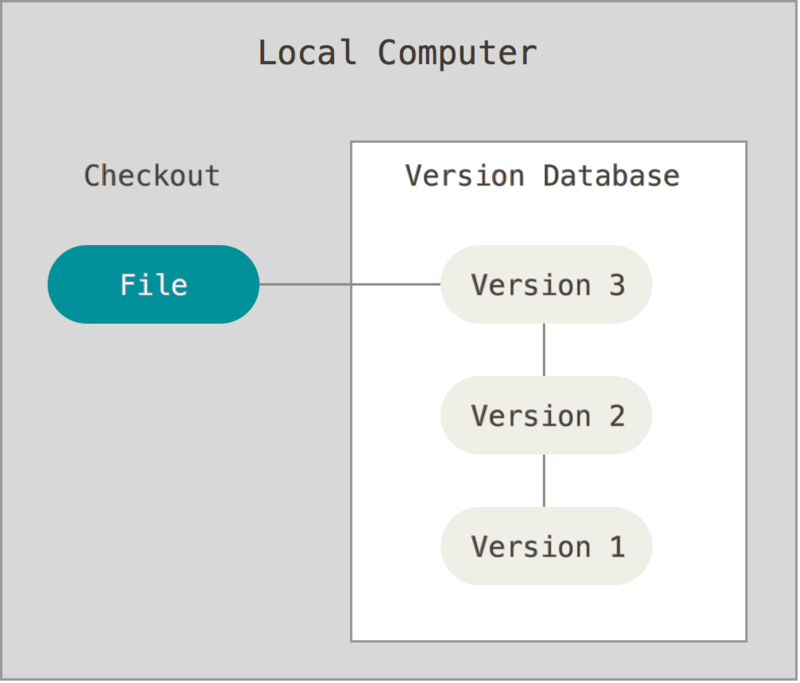
\includegraphics[width=0.5\textwidth]{Figures/lvcs.png}
  \end{center}
  \caption{Sistema de Control de Versionamiento Local. Fuente: \citep{PROGIT-Git-VCS}.}
  \label{LVCS}
\end{figure}

Después se dieron cuenta que seria bueno poder colaborar sobre las mismas versiones entonces se inventó lo que se conoce como Sistemas de Control de Versionamiento Centralizados los cuales permiten un alto grado de control y seguridad sobre quién puede editar y cuando puede editar que dentro de la base de datos de contenido ya que las mismas siguen un modelo arquitectónico cliente-servidor \citep{PROGIT-Git-VCS}. Eso ha resultado que en empresas grandes que necesitan desarrollar sistemas grandes en paralelo con un cierto grado de seguridad, les resulta bien usar un sistema de control de versionamiento de esta clase aunque esto está cambiando ya que las empresas están dándose cuenta que pueden optar por una solución híbrida \citep{CollabNet-Dist-or-Cent}. Ejemplos de estos CVCS son CVS, Subversión y Perforce. Pero el problema viene a ser que todo el repositorio tiene un solo punto de falla porque si cae el servidor o le pasa algo, se pone en riesgo la productividad continua de quien colabora y en el peor de los casos, la integridad del repositorio. Esta propiedad se puede ver en la figura \ref{CVCS} \citep{PROGIT-Git-VCS}.

\begin{figure}
  \begin{center}
  	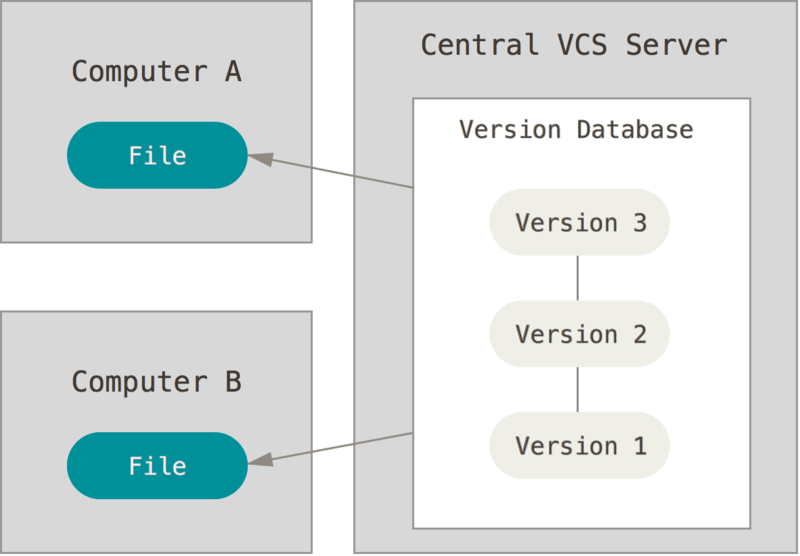
\includegraphics[width=0.5\textwidth]{Figures/cvcs.png}
  \end{center}
  \caption{Sistema de Control de Versionamiento Centralizado. Fuente:  \citep{PROGIT-Git-VCS}.}
  \label{CVCS}
\end{figure}

Con la explosión de desarrollo de software libre, hubo una necesidad de poder trabajar grandes cantidades de personas desconocidas en paralelo \citep{raymond1999cathedral}, y para resolver este problema y también la de integridad de datos que presenta el único punto de falla de los Sistemas de Control de Versionamiento Centralizado, se inventó Sistemas de Control de Versionamiento Distribuidos como Git, Mercurial, Bazaar y Darcs. Cada repositorio es un espejo de los demás en una arquitectura distribuida o red de iguales. Con esta arquitectura (mira figura \ref{DVCS}), ningún nodo viene a ser un punto de falla ya que se puede espejar entre cualquiera de ellos debido al hecho de que todos tienen una copia local de todo lo que tienen los demás \citep{PROGIT-Git-VCS}. 

\begin{figure}
  \begin{center}
      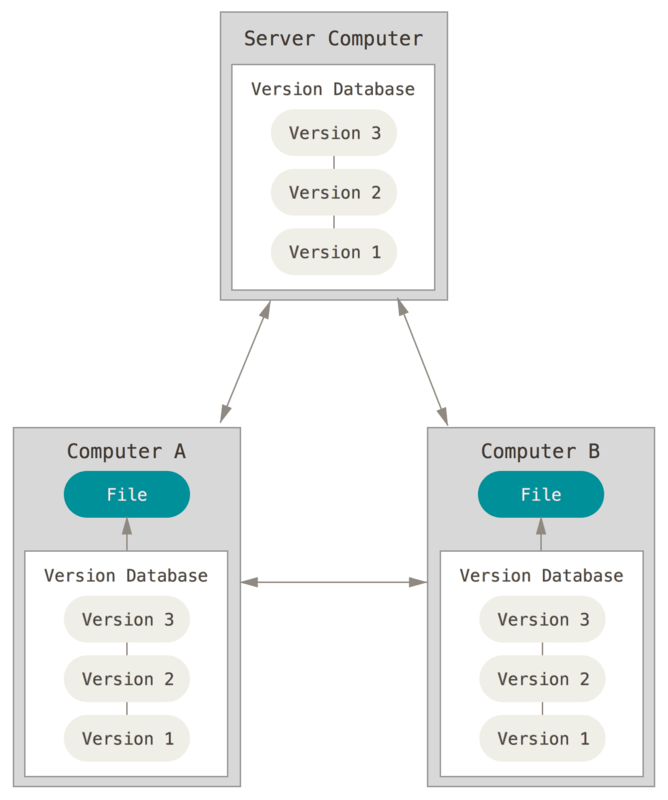
\includegraphics[width=0.5\textwidth]{Figures/dvcs.png}
  \end{center}
  \caption{Sistema de Control de Versionamiento Distribuido. Fuente: \citep{PROGIT-Git-VCS}.}
  \label{DVCS}
\end{figure}

\subsubsection{Git}
Git es un sistema de control de versiones distribuido que a diferencia de otros VCS guarda con cada versión una copia entera de los archivos modificados (otros sistemas de control de versionamiento saben guardar solo las diferencias entre versiones de forma incremental, mira la diferencia entre la figura \ref{VCS-Incremental} y la figura \ref{VCS-Backup}) \citep{PROGIT-Git-Intro}.

\begin{figure}
  \begin{center}
      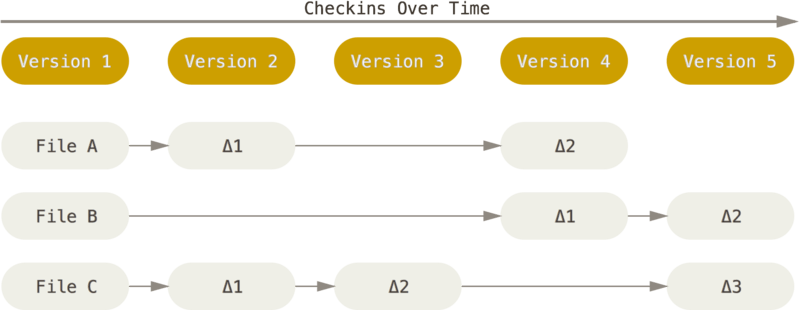
\includegraphics[width=\textwidth]{Figures/vcs-incremental.png}
  \end{center}
  \caption{Figura (VCS-Incremental). Un Sistema de Control de Versiones llevado de forma incremental (la manera en que muchos VCS funcionan). Fuente: \citep{PROGIT-Git-Intro}.}
  \label{VCS-Incremental}
\end{figure}

\begin{figure}
  \begin{center}
      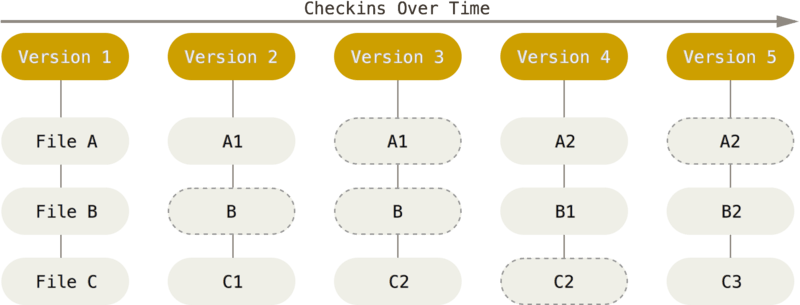
\includegraphics[width=\textwidth]{Figures/vcs-backup.png}
  \end{center}
  \caption{Un Sistema de Control de Versiones llevado con archivos enteros (la manera en que funciona Git). Fuente: \citep{PROGIT-Git-Intro}.}
  \label{VCS-Backup}
\end{figure}

Esto hace que Git se convierte más en como un pseudo sistema de ficheros que un simple VCS. Además significa mayor integridad de los datos guardados a costo de mayor consumo de almacenamiento. Trabaja de esta manera distribuida, es decir el repositorio existe en esta forma en todo lado donde se encuentra y por lo tanto la mayoría de operaciones de Git se puede realizar de manera local sin ninguna conexión de red \citep{PROGIT-Git-Intro}.
Volviendo al tema de integridad de datos, Git utiliza SHA-1 como algoritmo criptográfico para calcular los hash de cada cambio que se realiza en base a una combinación de qué información contiene el cambio, su metadata como autor, fecha, hora y fecha en adición a los SHA-1 de su(s) cambio(s) padre(s)\footnote{La mayoría de commits solo tienen un padre, pero aquellos que unen varios historiales, tienen dos padres} de tal forma que es difícil si no prácticamente imposible\footnote{Un equipo de investigación de Google y CWI Amsterdam ha encontrado una vulnerabilidad que recién publicaron y les permite atacar SHA-1 y encontrar colisiones hash \citep{Shattered-Paper}} para un atacante modificar el historial sin dejar evidencia de lo que se ha hecho. Por defecto funciona así \citep{PROGIT-Git-Intro}, pero si uno desea asegurar la integridad del historial aún más, se integra Git con GPG para ofrecer mayor seguridad ya que con eso se puede firmar digitalmente cambios realizados para demostrar su autenticidad \citep{PROGIT-Git-GPG}.

La mayoría de operaciones normales  que se hacen en Git no eliminan datos ya guardados en el repositorio previamente lo cual lo hace una buena herramienta para personas que recien esta entrando al mundo de Sistemas de Control de Versionamiento y permite que se pueda recuperar de la mayoría de errores que se puede cometer y una recuperación casi garantizado de datos “perdidos”. Eso es gracias en parte a la filosofía que se refleja en el diseño del mismo ya que una prioridad primordial era la integridad de los datos \citep{PROGIT-Git-Intro}.

Cada repositorio de Git trabaja con tres fases que son el directorio de trabajo donde se realiza cambios, una área de preparación donde se marca cambios listos para guardar y una base de datos junto un sistema de ficheros donde se guardan los cambios. Al saltarse entre versiones, se sobreescribe los contenidos del directorio de trabajo con lo que se extrae del sistema de ficheros que tiene los cambios guardados. Esas tres fases y su relación se puede ver en la figura \ref{Git-Fases} \citep{PROGIT-Git-Intro}.

\begin{figure}
  \begin{center}
      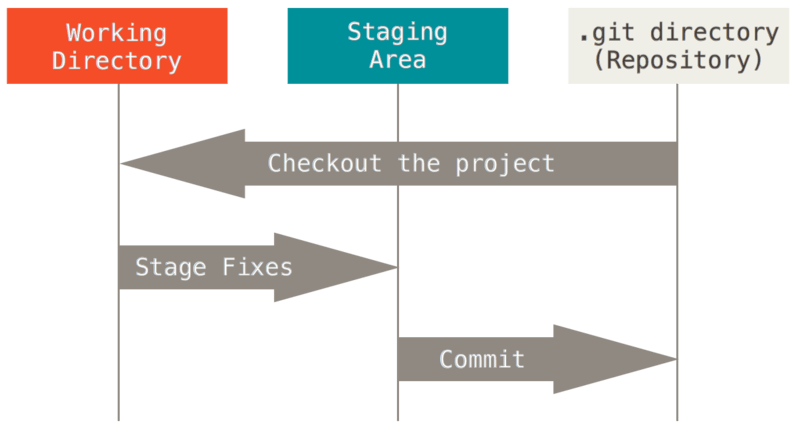
\includegraphics[width=0.5\textwidth]{Figures/git-fases.png}
  \end{center}
  \caption{Los tres fases de Git y sus relaciones. Fuente: \citep{PROGIT-Git-Intro}}
  \label{Git-Fases}
\end{figure}

\paragraph{GitLab}
GitLab es un servidor de Git ofrecido por GitLab Inc. Se ofrece en dos versiones: una versión gratis \citep{GitLab-Products} de código abierto liberado bajo el nombre GitLab Community Edition (GitLab CE) y una versión pagada que forma la línea principal de negocio de GitLab Inc. que lo venden bajo el nombre GitLab Enterprise Edition (GitLab EE) \citep{GitLab-About}. También proporcionan hosting de las mismas versiones alojados por ellos en GitLab.com (alli se puede usar GitLab EE gratis \citep{GitLab-GitLab.com} \citep{GitLab-Products}) y en GitHost.io (donde se puede arrendar servidores para alojar instancias de GitLab CE o EE y su respectivo infraestructura de apoyo \citep{GitHost.io}) \citep{GitLab-About}. Actualmente la Universidad Técnica Particular de Loja utiliza un servidor de GitLab CE como su instancia institucional de Git \citep{UTPL-GitLab}.

\subsubsection{Virtualización}
Virtualización es la creación de recursos virtuales en software para usar los mismos en lugar de un recurso físico. Este puede ser usado en áreas diversas como aplicaciones, servidores, almacenamiento y redes. Según la empresa VMware, que se dedica a vender productos de virtualización, la misma es la estrategia más efectiva para reducir costos de TI mientras que se aumenta la eficiencia y agilidad de un negocio de cualquier tamaño. Llegan a esta conclusión porque es tan común que se ha convertido en estándar industrial que solo se ocupa en entre 5\% y 15\% de la capacidad de los servidores debido a que se les pone solo un sistema operativo y aplicación a la vez. Virtualización permite resolver estas deficiencias en permitir la división lógica de equipos y distribuir estas partes donde más se los necesitan para aumentar la tasa de eficiencia y reducir la cantidad de recursos físicos necesarios. Con esta clase de tecnología, se puede reducir y en algunos casos eliminar tiempo fuera de servicio. Las facilidades de portabilidad y agilidad de ajustar recursos hace que se puede reducir los tiempos y costos de administración. Se domina hipervisor un software que gestiona virtualización \citep{VMWare-Virtualization}.

\begin{figure}
  \begin{center}
      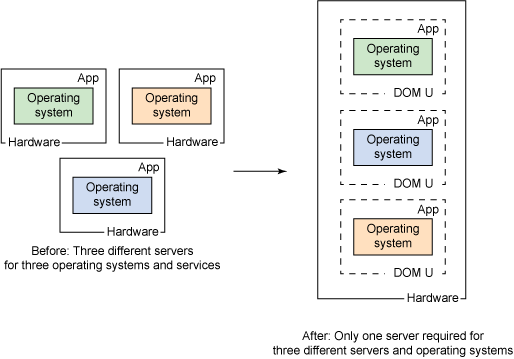
\includegraphics[width=0.5\textwidth]{Figures/ibm-virtualization.png}
  \end{center}
  \caption{Antes y después de virtualizar aplicaciones. Fuente: \citep{IBM-Hypervisors}.}
  \label{IBM-Virtualization}
\end{figure}

\paragraph{Las Máquinas Virtuales}
Una Máquina Virtual es una sistema computacional entera con sistema operativo y aplicación corriendo sobre recursos virtuales. Por lo tanto cada máquina virtual es completamente aislada e independiente de los demás de tal forma que se puede tener varios sistemas operativos y aplicaciones corriendo sobre un solo servidor físico. Eso permite tener varias características importantes:
\begin{description}
	\item[División de Recursos] Se puede dividir recursos físicos entre varios sistemas operativos corriendo sobre la misma máquina.
    \item[Aislamiento] Proveer mayor seguridad en prevenir o restringir acceso entre las varias máquinas virtuales.
    \item[Encapsulación de Persistencia] Todo el estado de la máquina virtual se lo puede guardar en archivos, los mismos que pueden ser sincronizados entre varios equipos o ubicaciones.
    \item[Independencia de Hardware] Se puede usar la máquina virtual en cualquier hipervisor que lo soporte.
\end{description}
Todo estas caracteristicas anteriores permiten la consolidación de servidores para utilizar menos servidores y cortar costos \citep{VMWare-Virtualization}.

\paragraph{Virtualización de Servidores}
Con virtualización de servidores, se puede reducir el número de servidores necesarios dentro de una granja, especialmente cuando los mismos son miembros de un cluster que realiza balanceo de recursos frente su carga para optimizar la eficiencia de toda la granja \citep{VMWare-Virtualization}.

\paragraph{Virtualización de Redes}
Con virtualización de redes se puede simular todo el tráfico y funcionamiento de una red sin mayor retardo. Se puede virtualizar interfaces de red, los switch, routers, cortafuegos, balanceadores de carga, VPNs y más. Como los otros tipos de virtualización, esta ofrece los mismos beneficios de independencia, costos y escalabilidad \citep{VMWare-Virtualization}.

\paragraph{Virtualización de Escritorios}
Virtualización de Escritorios se trata de usar recursos centralizados para dar escritorios de trabajo a usuarios remotos. Esto permite a cualquier organización reducir sus gastos tecnológicos debido a que el mismo permite menor inversión en tecnología para la misma cantidad de usuarios mientras al mismo tiempo facilita temas de administración de los equipos de los empleados en una organización y seguridad de la información de la misma \citep{VMWare-Virtualization}.

\subsubsection{Hipervisores}
Un hipervisor es una capa intermedia de software que gestiona la interacción entre lo virtualizado y hardware o otro software que ayuda realizar las peticiones de lo virtualizado \citep{VMWare-Virtualization}. De la misma manera, el mismo hipervisor se encargan de seguridad para asegurar que lo que sea virtualizado no pueda salir de su ambiente y atacar otras partes virtualizados o no virtualizados \citep{VMWare-HypervisorSecurity} \citep{IBM-KVM-Security}.

\begin{figure}
  \begin{center}
      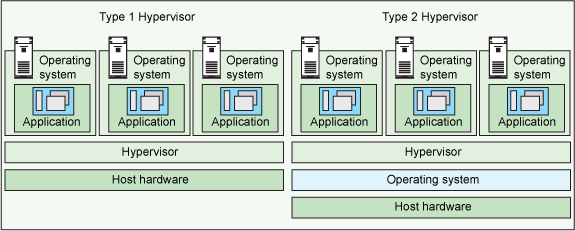
\includegraphics[width=\textwidth]{Figures/ibm-hypervisortypes.png}
  \end{center}
  \caption{Tipos Clásicos de Hipervisor.} \center{Fuente [IBM-Hypervisors].}
  \label{IBM-HypervisorTypes}
\end{figure}

\paragraph{Hipervisores de Tipo 1}
Un Hipervisor de Tipo 1 se ejecuta directamente sobre hardware física \citep{IBM-Hypervisors} y por lo tanto puede llegar a conseguir mejor rendimiento y seguridad pero a un costo de requerir en muchos casos mayor configuración y administración para poder alcanzar su rendimiento óptimo.

\subparagraph{Xen}
Xen es un hipervisor de tipo 1, que corre directamente sobre hardware. Es el único hipervisor de su clase que es completamente disponible bajo una licencia abierta y forma una base por muchas aplicaciones comerciales y no comerciales como virtualización de servidores, IaaS, virtualización de escritorios, aplicaciones de seguridad, y dispositivos embebidos. Dentro del mercado, es la tecnología detrás de las nubes más grandes \citep{Xen-Project-Overview}.
 
Para el mismo, se considera las siguientes características:
\begin{itemize}
	\item La implementación y uso de un micronúcleo que ocupa un mínimo de memoria y tiene interfaz externa limitado el cual ayuda proporcionar mayor seguridad y estabilidad en comparación con otros hipervisores. El hipervisor en si esta escrito en menos de 150 KLOCs que para un sistema operativo es muy liviano. Puede ser tan liviano porque no necesita tener conocimientos de operaciones de entrada/salida como redes o almacenamiento debido a que Dom0 se encargará de estos tareas. Al mismo tiempo, las demás máquinas virtuales no son privilegiados y siempre tienen que comunicarse con Dom0 para realizar cualquier operación con respecto al hardware físico. Por lo tanto la muerte del Dom0 es fatal para todas las máquinas que están en el Hipervisor.
    \item La arquitectura de Xen ocupa una maquina virtual que se domina Dom0 el cual contiene todos los drivers para el hardware y también la herramientas necesarias para ejercer control sobre todo el hipervisor. Estás funcionalidad son independientes del sistema operativo motivo por el cual que el sistema operativo residente del Dom0 puede ser Linux, una BSD, OpenSolaris, etc\ldots
    \item Como los drivers que controlan hardware física existen dentro de una máquina virtual, se los consideran drivers aislados. En caso de que pase algo, solo hay necesidad de reiniciar la máquina afectada, el resto del sistema puede seguir funcionando normalmente.
    \item Con una tecnología llamada paravirtualización, en lugar de optimizar al nivel de hipervisor se optimiza los sistemas operativos que son virtualizados para de esta manera mejorar su rendimiento incluso en hardware que no tiene soporte para virtualización. \citep{Xen-Project-Overview}.
\end{itemize}

\begin{figure}
  \begin{center}
      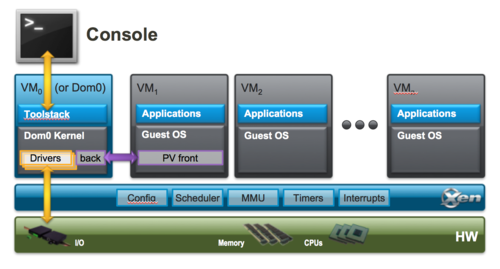
\includegraphics[width=\textwidth]{Figures/arq-xen.png}
  \end{center}
  \caption{La arquitectura de Xen. Fuente: \citep{Xen-Project-Overview}.}
  \label{arq-xen}
\end{figure}

\paragraph{Hipervisores de Tipo 2}
Un Hipervisor de Tipo 2 se ejecuta por encima de un sistema operativo que le ayuda con su gestión interna como si fuera una aplicación más \citep{IBM-Hypervisors} lo que hace este tipos de hipervisores más lentos que hipervisores de tipo 1 (por tener un mayor número de capas y también por virtualizar partes del hardware) pero a su vez más fáciles de configurar y administrar. El mismo hecho de ejecutar por encima de un sistema operativo también vulnera la seguridad de todo el sistema en proveer un superficie de ataque más grande para actores maliciosos.

\subparagraph{Qemu-KVM}
QEMU es un proyecto de software abierto con el fin de crear un emulador y virtualizador de procesadores de varias arquitecturas para una variedad de sistemas operativos. Permite el uso de backends como KVM o Xen para dar rendimiento casi nativo \citep{QEMU}. Aunque su despliegue normal requiere un sistema operativo, basado en Linux, intermedio debido a que es un módulo que se integra directamente en el núcleo de la misma sistema operativo, Wilson et. al. consideran KVM como un hipervisor de tipo 1 debido a sus características y implementación a bajo nivel cerca al nivel hardware física, mientras que su arquitectura lo hace aparecer como un hipervisor de tipo 2, que es como se lo está considerando aquí dentro del contexto de este trabajo (mientras que otros autores lo consideran un hipervisor de tipo 1.5, ni uno ni el otro si no algo híbrido dentro de la taxonomía de hipervisores). KVM es la “hipervisor estratégica para IBM” debido a (1) su bajo costo por ser tecnología completamente abierta, (2) su alta evolución y madurez, (3) alta evolución y madurez de Linux (su tecnología fundamental atras), (4) eficiencia y rendimiento alto, (5) una comunidad de desarrollo muy activa y responsable frente fallos de seguridad, (6) la idea de que muchos ojos viendo código lo hace más seguro\footnote{Uno de las características principales de Código Abierto}, (7) varias tecnologías de seguridad que integra que falta la competencia, (8) mayor flexibilidad que ofrece frente otros hipervisores competidores y (7) control que IBM puede ejercer sobre el proyecto de KVM \citep{IBM-KVM-Security}.

\begin{figure}
  \begin{center}
      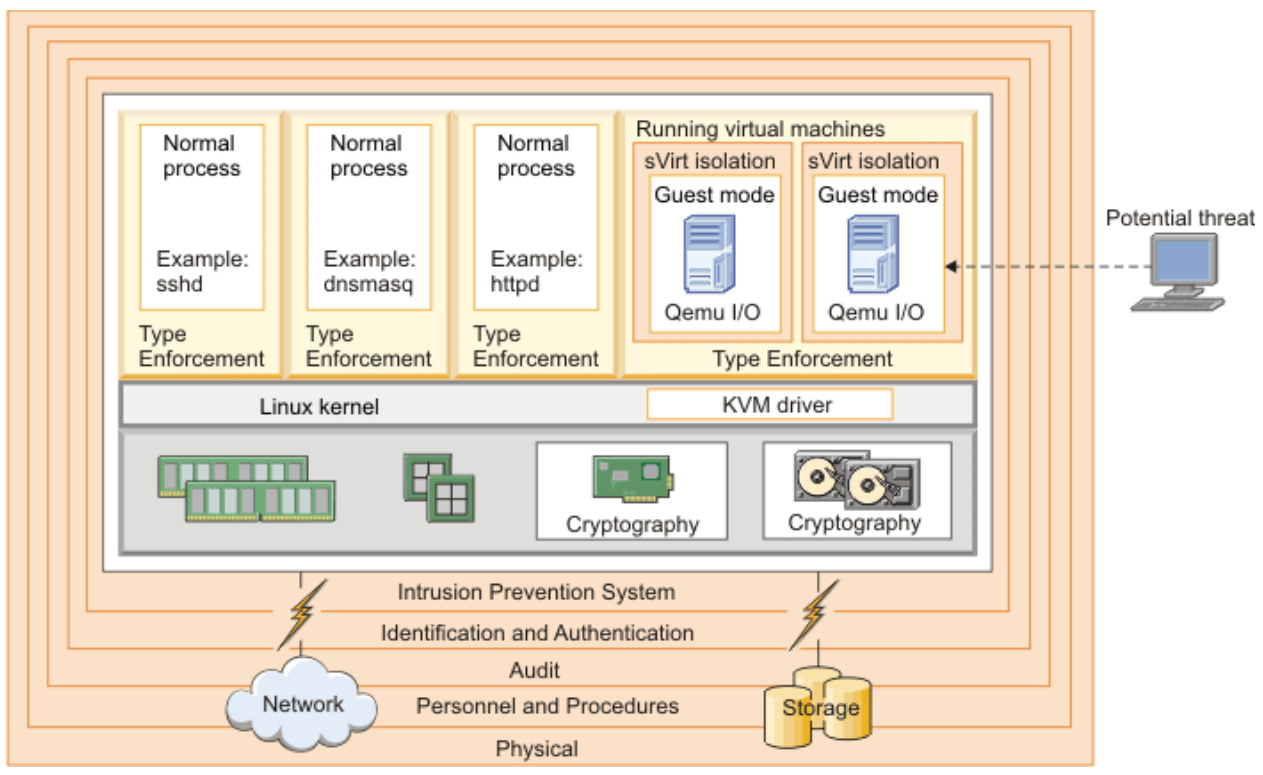
\includegraphics[width=\textwidth]{Figures/kvm-arq.png}
  \end{center}
  \caption{Arquitectura de KVM/QEMU. Fuente: \citep{IBM-KVM-Security}.}
  \label{KVM-Arq}
\end{figure}

\subparagraph{VirtualBox}
VirtualBox es un hipervisor para virtualización de arquitecturas estándar x86 y x86\_64 tanto para uso casero como uso empresarial. Para ello ofrece muchas características, rendimiento optimizado, y un gran número de sistemas operativos que soporta tanto para virtualizar como para ser virtualizados todo bajo una licencia de software libre, la GPL versión 2 \citep{VirtualBox}. Su arquitectura de ser montado encima de cualquier sistema operativo y apoyarse en ello para realizar operaciones por parte de un sistema operativo y hardware virtualizado hacen este hipervisor un ejemplo clásico de un hipervisor de tipo 2.

\paragraph{Virtualización a Nivel de Sistema Operativo (Contenerización)}
Desde la antes de la incepción de los sistemas Linux, los sistemas de la familia Unix han tenido un mecanismo de aislamiento conocido como chroot el cual genera un espacio aislado de usuario para contener alguna aplicacion o varias aplicaciones mientras que todos siguen compartiendo el mismo sistema operativo o kernel por detrás. La tendencia de contenerización que existe hoy en día sigue por la misma línea pero lo implementa de una forma aún más avanzada. Eso permite a muchos usuarios que se desconfían mutuamente unos en otros utilizar el mismo hardware mientras que al mismo tiempo quedan completamente aislados unos de otros con menor impacto al rendimiento o una necesidad de hardware que soporta la carga adicional que virtualizacion genera \citep{Teimouri-Davoud-OS-level-virt}, mira la figura \ref{que-son-contenedores}. Algunos sistemas de este tipo de aislamiento que son populares hoy en día son:
\begin{itemize}
	\item chroot
    \item Docker
    \item LXC
    \item LXD
    \item Linux-VServer
    \item OpenVZ
    \item Solaris Containers
    \item FreeBSD jail
    \item Hyper-V containers (Microsoft)
    \item Photon (VMware)
    \item vSphere Integrated Container (VMware)
    \item Windows Containers (a partir de Windows Server 2016)
\end{itemize}

\begin{figure}
  \begin{center}
      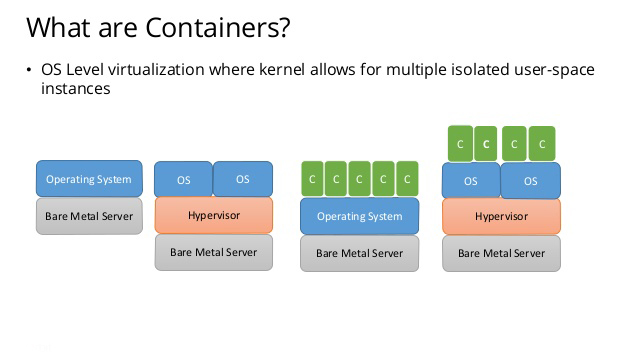
\includegraphics[width=\textwidth]{Figures/que-son-contenedores.jpg}
  \end{center}
  \caption{Un concepto básico de que son los contenedores \citep{Teimouri-Davoud-OS-level-virt}.}
  \label{que-son-contenedores}
\end{figure}

\begin{figure}
  \begin{center}
      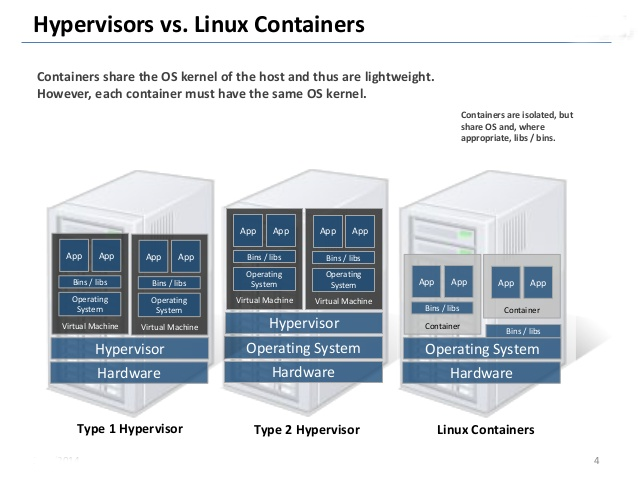
\includegraphics[width=0.75\textwidth]{Figures/differencia-hipervisores-contenedores.png}
  \end{center}
  \caption{La diferencia que abarca contenedores de los tipos de hipervisores \citep{Teimouri-Davoud-OS-level-virt}.}
  \label{differencia-hipervisores-contenedores}
\end{figure}

Debido al hecho de que muchas veces cada máquina virtual necesita su propio hardware virtual y también sistema operativo, se termina consumiendo mucho más RAM y ciclos de CPU de tal manera que un servidor típicamente puede soportar dos a tres veces más servicios si están en contenedores en lugar de si son virtualizados \citep{Teimouri-Davoud-OS-level-virt}. La diferencia se puede ver en la figura \ref{differencia-hipervisores-contenedores}.

\begin{figure}
  \begin{center}
      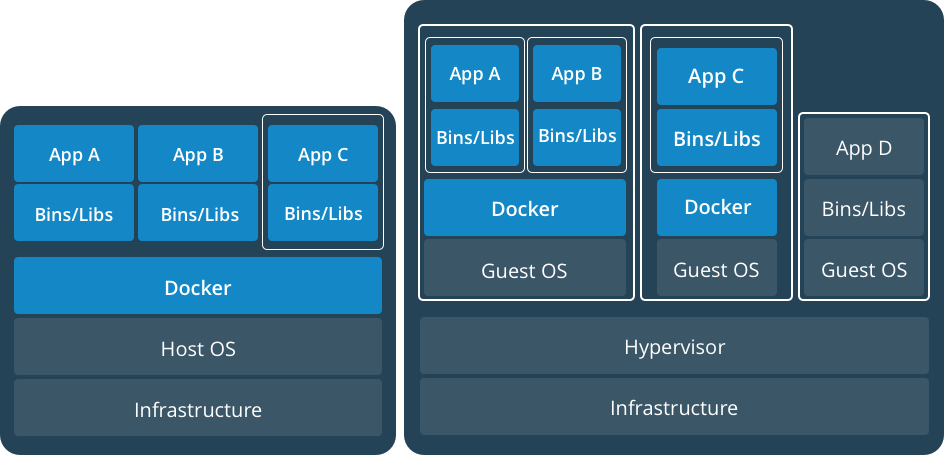
\includegraphics[width=0.75\textwidth]{Figures/contenedores-vms.png}
  \end{center}
  \caption{La diferencia entre contenedores nativas y dentro de una máquina virtual. \citep{Docker-Containers}}
  \label{contenedores-vms}
\end{figure}

Entre las ventajas de contenedores está que permiten tener ambientes aislados livianos para prevenir conflictos de dependencias y estandarizar versiones utilizadas en ambientes de desarrollo y producción mientras que al mismo tiempo requieren mucho menos recursos que una máquina virtual. Las mismas se pueden levantar casi instantáneamente a diferencia de máquinas virtuales que requieren tiempo para arrancarse. Como se puede ver en la figura (contenedores-vms), también se puede tener un motor de contenedores dentro de una máquina virtual, el cual ofrece beneficios como mayor aislamiento (seguridad) y flexibilidad al momento de migrar aplicaciones entre servidores \citep{Docker-Containers}.

La estandarización que ofrece la contenerización ayuda abstraer sistemas operativos que están en los servidores (permitiendo mayor flexibilidad de despliegue),  permite mayor escalabilidad si la aplicación es diseñada para eso, es fácil de versionar dado que los archivos de configuración que describen los contenedores muchas veces son de texto plano y es muy orientado a arquitecturas compuestas por servicios como SOA o las arquitecturas de Microservicios debidos a que estas ya tienen componentes donde es fácil saber dónde poner la frontera de cada contenedor \citep{DigitalOcean-Docker-Ecosystem}.

Para tener seguridad adicional, también se puede ocupar contendores dentro de máquinas virtuales aisladas como se puede observar en la figura \ref{contenedores-vms} \citep{Docker-Containers}.

\subparagraph{Docker}
Docker es una plataforma más popular hoy en dia para contenedores. Se puede usar para eliminar problemas de dependencias entre equipos de desarrolladores, para aumentar la capacidad computacional de equipos y también para desplegar de una forma más ágil, rápida y segura. Con contenedores de Docker, toda la complejidad está dentro del contenedor, facilitando su compilación, la forma en que son compartidos y ejecutados, lo que hace fácil que cualquier persona que tenga los archivos de configuración necesarias puede levantar la aplicación en minutos en lugar de en horas \citep{Docker-What-Is}.

La arquitectura de Docker permite funcionar con cualquier tecnología. La estandarización y facilidad que ofrece permite mejor colaboración entre miembros de un equipo. Por defecto Docker se trata de ser lo más seguro, flexible y extensible posible mientras que al mismo tiempo no necesitar cambios para que un proveedor de software no necesita realizar cambios ni casarse con la tecnología \citep{Docker}.


\subsubsection{Protocolo de Túnel}
Un túnel es una técnica de permitir acceso remoto a recursos en una red a los cuales normalmente no se tendría acceso desde afuera. Se puede realizar esto en la capa 2 de redes con los protocolos como L2TP, PPTP y L2F quienes buscan encapsular paquetes previo a su viaje entre redes y desencapsularlos en ambos lados del túnel. Puede ser una solución económica para todos los involucrados ya que permite montar varios VPNs en la misma infraestructura física \citep{Cisco-Tunneling}. Los protocolos de túnel saben transmitir dos tipos de mensajes, aquellos paquetes que encapsulan datos y otros paquetes auxiliares que definen las reglas de reenvío \citep{Kaspersky-Tunneling}. Por esta razón y también la tendencia de estos protocolos de proteger los datos que transmiten con encriptación resulta en una velocidad de transferencia de datos menor que simple envío directo. Algunos otros protocolos de encapsulación buscan reemplazar TCP y UDP en la capa 4 pero su funcionalidad de transportar paquetes entre redes, que de ninguna otra forma serían conectados, es igual y forma un tipo de VPN. Los protocolos SSH y IPSec también tienen esas funcionalidades. Así se puede lograr reenviar puertos para utilizar servicios internos como portales internos de una institución o convertir una máquina con Linux/UNIX en un servidor gráfico para “terminales tontos” \citep{ENP-Tunneling} como los días clásicas de la infancia de UNIX \citep{GeerlingJeff-History-Remote-Access}. Aunque su poder y seguridad lo ha hecho un herramienta común entre profesionales que trabajan con redes \citep{ENP-Tunneling}, también por su misma naturaleza se puede ocultar tráfico y por lo tanto ahora es común que malware y actores maliciosos utilizan esos mismos protocolos para esconder su actividad y realizar actos malvados con un menor riesgo de ser detectados en tiempo real. Por lo tanto, para usuarios normales, se recomienda limitar el uso de estos protocolos \citep{Kaspersky-Tunneling}.

\subsubsection{Criptografía}
Criptografía es una ciencia de proteger datos comunicados que han sido utilizado por miles de años para comunicarse de tal forma que el emisor y receptor pueden enviar y recibir mensajes pero personas intermedias no pueden entender los mensajes en tránsito. Tiene aplicaciones militares, financieros y también en el ámbito tecnológico, sobre todo para el internet, entre otras aplicaciones para los cuales ha sido usado a lo largo de la historia. Cifrar es el acto de ocultar datos y decifrar es la acción opuesta para devolverlos a su estado original \citep{Khanacademy-What-is-Cryptography}.

\paragraph{Criptografía Asimétrica}
Con la introducción de redes y la necesidad de encriptar comunicaciones entre personas quienes nunca se ha habían reunido para llegar a un acuerdo de que usar de llave criptográfica para comunicaciones, se necesitaba una manera de llegar a este acuerdo sin que ningún agente intermedio también sepa la llave criptográfica resultante del acuerdo y por lo tanto se introdujo la necesidad de la criptografía asimétrica \citep{Khanacademy-RSA-1}. Para cumplir con este requisito, el receptor genera una llave privada y llave pública, los cuales son operaciones inversas y publica su llave pública para todos que deseen comunicarse con el mismo. Ahora quienes quieren comunicar con el dueño de la par de llaves ocupan su llave pública para cifrar el mensaje y lo envían. Solo con la llave privada se puede descifrar el mensaje y así como el dueño es el único que tiene esta llave, sólo él puede leer los mensajes enviados \citep{Khanacademy-RSA-1}.

\subsubsection{SSH}
En la infancia de la computación, solo habían computadores centralizados en instituciones grandes. Aún no existía el Internet ni las  redes, estaban en su infancia. Poco a poco se introdujo la idea del terminal tonto y con ello el acceso por varios usuarios a estas mismas computadoras centralizados sobre un LAN institucional. De aquí proviene el concepto de control remoto y en aquella época de redes bien controlados y cableados, no hubo mucho riesgos de seguridad entonces por lo tanto el protocolo de esos tiempos fue Telnet, donde todos los datos, incluyendo usuarios y contraseñas son enviados en texto plano. Con el tiempo se volvió más económico y ubicó la tecnología de tal forma que, junto al Internet, se estaba empezando a usar Telnet en redes de desconocidos y generando situaciones potencialmente maduros para ataques clásicos de análisis o incluso modificación de paquetes en tránsito. Fue frente esta realidad que un Finlandés diseñó e implementó el protocolo SSH \citep{GeerlingJeff-History-Remote-Access}. OpenSSH es una implementación abierta y libre \citep{OpenBSD-OpenSSH-Features} del protocolo SSH, que como se define el protocolo, cifrar su tráfico para proteger contra espionaje, robo de conexión y otros ataques que afectan otros protocolos de una naturaleza similar. El proyecto OpenSSH, para ofrecer la mayor funcionalidad posible tiene integrado funcionalidades de túneles seguros, varios métodos de autenticación, y opciones avanzadas de configuración. Adicional a esto ofrece una variedad de herramientas para la gestión de sus funcionalidades con clientes como los comandos ssh, scp y sftp, gestión de llaves con comandos como ssh-add, ssh-keysign, ssh-keyscan, y ssh-keygen, en adición a servicios en segundo plano como sshd, sftp-server y ssh-agent \citep{OpenSSH}. Hoy en día se puede utilizar SSH para cifrar conexiones en redes que de ninguna otra forma serían cifradas, reenviar tráfico de un servidor gráfico X11 (para tener varios terminales gráficos en una sola máquina servidor \citep{ENP-Tunneling}), reenvío de puertos sobre un canal seguro, fuerte mecanismos de autenticación como claves de único uso y llaves de criptografía asimétrica, reenvío de agentes de autenticación, interoperabilidad con otras versiones y implementaciones del protocolo SSH, y la opción de activar compresión y descompresión de datos en tiempo real para optimizar el consumo de recursos en red \citep{OpenBSD-OpenSSH-Features} \citep{OpenBSD-manpages-SSH}.

\paragraph{Túnel de SSH}
SSH es un protocolo de túnel muy popular \citep{Kaspersky-Tunneling} ya que ofrece mucha flexibilidad para las mismas \citep{OpenSSH} y alta seguridad desde la autenticación para iniciar la conexión y para los datos transferidos en dentro de la conexión \citep{OpenBSD-OpenSSH-Features}. Su facilidad de uso permite con rapidez levantar mini VPNs de un puerto para acceder a puertos de otros equipos los cuales normalmente no serían disponibles, por ejemplo acceder servicios que solo son disponibles en un intranet \citep{ENP-Tunneling}.

\subsubsection{SSL}
SSL es un estándar tecnológico para cifrar tráfico \citep{info.SSL.com-SSL} \citep{GlobalSign-SSL} de protocolos que normalmente no son cifrados por ejemplo HTTP, SMTP e IMAP. Esto se hace con un fin de proteger datos sensitivos transferidos (en adición a asegurar su integridad \citep{info.SSL.com-SSL}) entre un cliente y servidor, los cuales normalmente se transfieren en texto plano y podrían ser leídos por cualquier agente intermedio. El proceso de comunicación se puede encontrar en la figura \ref{SSL-Proceso}. Para iniciarse la conexión cifrada, primero el cliente pide que el servidor se identifica (1) con la llave pública que forma parte de su certificado (2). Una vez que lo tiene, el cliente procede a validar el certificado para ver si confía en su origen (a través de firmas digitales por autoridades centrales) y en caso de que haya confianza, se procede a generar una llave criptográfica para la sesión, lo cual se lo transmite cifrada al servidor con la llave pública del mismo (3). El servidor descifra la clave de sesión con su llave privada de su certificado, avisa el cliente que la transacción ha sido exitosa (4) y ambos proceden a transferir los datos adecuados, cifrados con la llave de sesión que tanto cliente como servidor comparten (5) \citep{DigiCert-SSL}.

\begin{figure}
  \begin{center}
      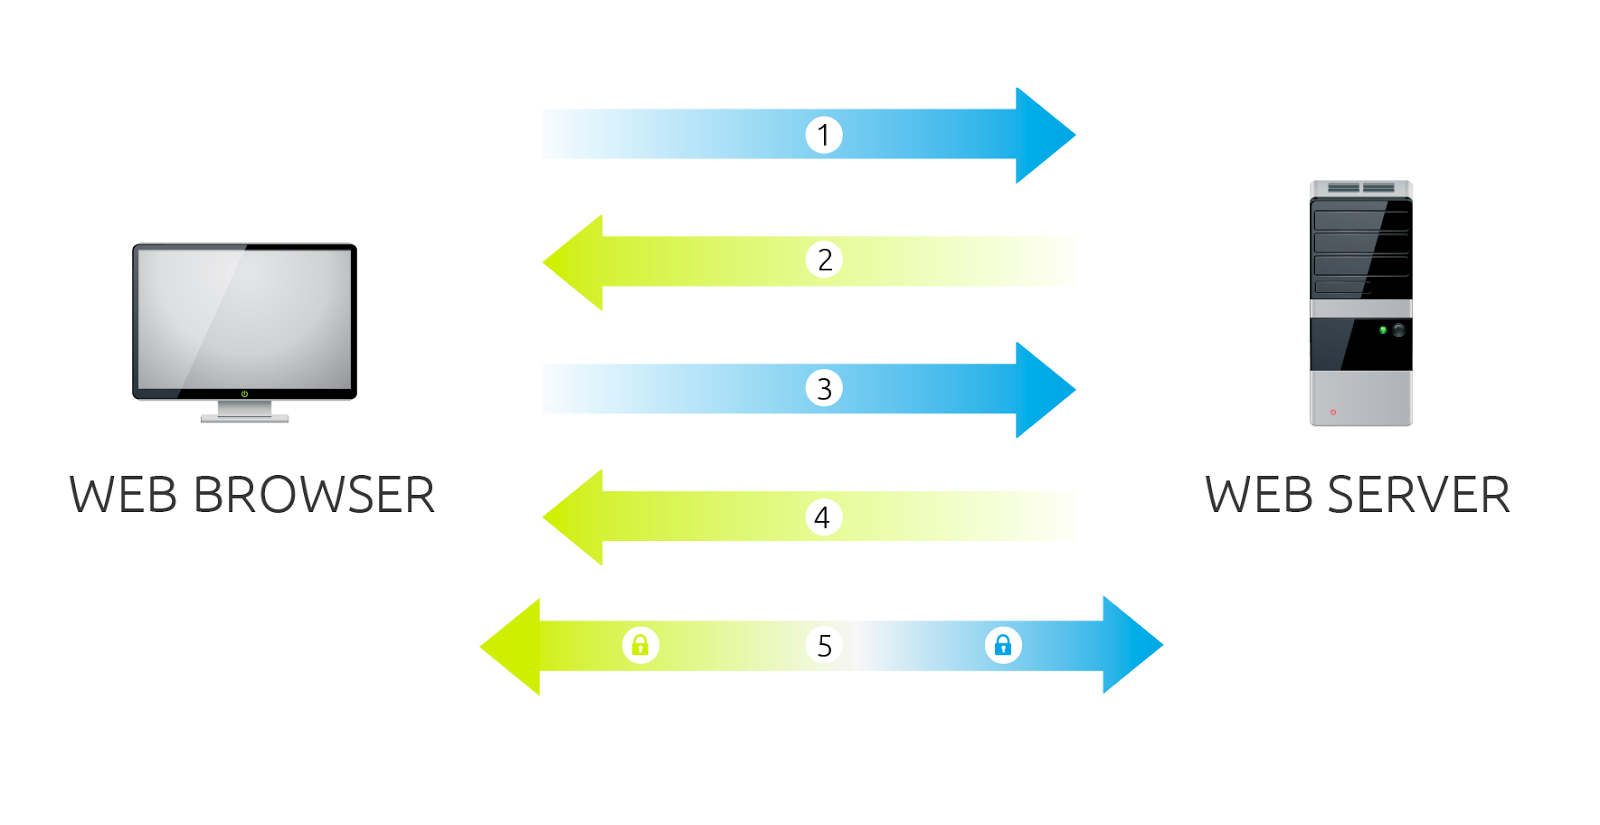
\includegraphics[width=\textwidth]{Figures/ssl-proceso.png}
  \end{center}
  \caption{El proceso para comunicación con el protocolo SSL. Fuente: \citep{DigiCert-SSL}}
  \label{SSL-Proceso}
\end{figure}

Para ayudar con el proceso de validación, el certificado SSL sabe contener detalles como la llave pública del servidor, el nombre de dominio, nombre de empresa, dirección, ciudad, estado o provincia y país. Es firmado por un autoridad de certificados para dar confianza a los clientes que revisarán el certificado \citep{info.SSL.com-SSL}. Antes de firmar un certificado, una autoridad de certificados primero valida la identidad del servidor que ha realizado la petición para el certificado para que más adelante puede confirmar a clientes que es el mismo servidor \citep{GlobalSign-SSL}.

\paragraph{TLS}
Cuando llegó la versión 4.0 de SSL, se cambió de nombre a TLS versión 1.0 \citep{DigiCert-SSL} para señalar un fuerte cambio de seguridad en cómo se manejan los casos de uso que pueden causar fallos de seguridad en antiguas versiones de SSL como POODLE, DROWN y BEAST que dejan la seguridad que promete SSL inútil y peligroso (ya que las mismas prometen seguridad falsa) \citep{LuxSci-SSL-vs-TLS} \citep{GlobalSign-SSL-vs-TLS}.

\subsection{Tecnologias de la Web}

\begin{table}[h!]
    \begin{tabular}{|p{0.15\textwidth}|p{0.8\textwidth}|}
    	\hline
        Concepto & Definición \\
    	\hline
        URI & Una URI identifica de forma única un recurso que existe en una red como el Internet \citep{Webopedia-URI}. Como se define en el RFC 3986, debe consistir de forma genérica en un:
        \newline
[protocolo de acceso][usuario][clave][dominio][ruta de recurso][parámetros de acceso al recurso]
		\newline
Donde usuario, clave son opcionales y la ruta del recurso y sus parámetros también pueden ser opcionales o innecesarios en casos de protocolos que no requieren el mismo \citep{RFC3986}. \\
        \hline
    	HTTP & HTTP es el protocolo con el cual se intercambia información como peticiones y datos con páginas web en el World Wide Web. Usa un esquema de códigos de error para comunicar tipos de sucesos que pueden ocurrir con el uso del protocolo \citep{ComputerHope-HTTP}. Dentro del protocolo HTTP, se usa verbos que son comandos que dicen que tipo de operación quiere hacer un cliente con relación a un servidor web. HTTP es conocido como un protocolo sin estados ya que dentro del protocolo se desconoce acciones anteriores que se ha tomado en la interacción cliente/servidor \citep{Webopedia-HTTP}. Algunas tecnologías adicionales de la web se muestran en la tabla (tecnologias-web). \\
        \hline
        HTTPS & HTTPS utiliza el estándar SSL y ahora TLS para cifrar conexiones HTTP entre un cliente y servidor \citep{ComputerHope-HTTP}. \\
        \hline
        API REST & Un API REST es un estilo arquitectónico donde se construye encima del protocolo HTTP para orientar el mismo protocolo a manejar estados. Este mismo estilo arquitectónico se orienta a escalabilidad y sistemas de software grandes \citep{Webopedia-REST}. \\
        \hline
        HTML & HTML es el lenguaje de autoría para páginas en la web. Usa una combinación de cientos de etiquetas predefinidas para definir estructura, formato y posición de contenido \citep{Webopedia-HTML}. \\
        \hline
        CSS & CSS es un lenguaje que permite definir estilos de cómo se presentará HTML. Se dice que son hojas de estilo en cascada porque se puede aplicar varios de ellos “en cascada” a una página de HTML \citep{Webopedia-CSS}. \\
        \hline
        JavaScript & JavaScript es un lenguaje de programación que tiene un fin de permitir que páginas de HTML sean dinámicas y pueden interactuar con el usuario en tiempo real \citep{Webopedia-JavaScript}.. \\
        \hline
    \end{tabular}
	\caption{Algunos de las tecnologías que son importantes en la funcionamiento de la web.}
    \label{tecnologias-web}
\end{table}

El cuadro \ref{tecnologias-web} presenta conceptos de varias tecnologías que existen en la web hoy en dia.

\pagebreak

\section{Trabajos Relacionados}
Dentro de la temática de este trabajo de titulación es importante entender trabajos relacionados los mismos que son analizados para en base a ellos entender investigaciones que ya se han realizado y de esta forma aprender de ellos. A continuación se mencionan los siguientes:

\subsection{GitEduERP}
En un trabajo reciente del autor con sus colegas, Marcelo Bravo y Priscilla Vargas, en la Universidad Técnica Particular de Loja, y frente el problema de necesitar ofrecer una ambiente de programación a estudiantes en línea, se realizó un editor de código en línea con sistema de permisos y la capacidad de compartir entre usuarios en un backend de Django y utilizando una librería ACE liberado por Cloud9 IDE que guardaba código editado en una instancia de GitLab CE. Además ofrece chat en línea con una liberia TogetherJS. El resultado era un prototipo que guardaba snippets en GitLab y permite compartir código de una manera muy primitiva entre usuarios. Se llevó el codigo editado en un sistema de control de versiones interna, usando MongoDB. Entre los problemas que se dieron era una falta de tiempo para el proyecto y una alta nivel de complejidad para el mismo lo cual no permitía que se lo termina según su alcance propuesta \citep{UTPL-GitEduERP}.

\subsection{Sistema de Encuestas Online}
Para mejorar temas de business analytics, se trató de diseñar procesos de negocio para realizar colección de datos en tiempo real a través de encuestas y analizar las mismas con un fin de ayudar la toma de decisiones estratégicas de negocio en tiempo real. Plantearon soluciones con un fin de optimizar tiempos y recursos a través del uso de soluciones tecnológicas \citep{UTPL-Thesis-Encuestas-Online}.

\subsection{Metodología de Enseñanza con la Web 2.0}
Se buscó utilizar la manera en que la moda de lectura-escritura en la Web 2.0 se podría crear cursos interactivos con estudiantes online como base de una nueva metodología de enseñanza. Destaca esos temas desde el punto de vista de ingeniería en sistemas para proporcionar soluciones netamente técnicas y estratégicas para dar el mejor aporte posible a quienes deseen implementar un sistema de este tipo \citep{UTPL-Thesis-Edu-Web-2}.

\subsection{Xen Web-based Terminal for Learning}
Los autores, Abdullah Almurayh y Sudhanshu Semwal de IAENG\footnote{International Association of Engineers}, propusieron e implementaron una arquitectura de cliente-servidor para la distribución de recursos educativos y en el proceso enseñar a estudiantes de Linux, programación orientada a la nube y gestión de nubes/servidores. Su aplicación web ofrece terminales SSH donde cada estudiante y docente disponía de una máquina virtual de tal forma que tenían su propio ambiente con permisos de superusuario y al mismo tiempo eran aislados de la infraestructura real y de los demás usuarios, motivo por el cual se podía dar una solución flexible y a su vez segura.

Como hipervisor ocuparon un sistema de Xen que controlan remotamente con su servidor de aplicación (servidor web). El enfoque del trabajo era garantizar seguridad mientras que al mismo tiempo dar ambientes con permisos completos donde estudiantes pueden experimentar y aprender sin restricciones mientras al mismo tiempo ser aislados y prevenir el mal uso o de alguna forma maliciosa.

La parte de seguridad se implementó con un validacion de comandos y eliminación de caracteres especiales que se podrían usar para escapar las restricciones establecidas previamente. De esta forma se logró realizar un sistema útil para administradores, docentes y estudiantes dentro del ámbito educativo. El sistema solo se implemento un comando, xe, para gestión del hipervisor Xen atrás y los autores dejaron como trabajo futuro mejorar la seguridad a futuro debido a que no lo vean como algo completo la seguridad actual \citep{almurayh2014xen}.

\section{Sistemas Similares}
De la misma manera que se analiza la parte de trabajos relacionados, es importante conocer también el contexto actual del mercado para ver las alternativas que ofrece la competencia y saber si ya hay alguna solución que sea de mayor beneficio a la universidad que el mismo sistema que se plantea (y por tal razón sería más factible implementar dicha solución en lugar de desarrollar algo nuevo). Se presenta a continuación las iniciativas investigadas:

\subsection{Repl.it}
Repl.it es una plataforma en línea, desarrollado por Neoreason Inc., para escribir y probar código en tiempo real como un IDE en línea. Su producto tiene un componente educativo que permite integración con otros sistemas de aprendizaje, organización por aulas, texto que guía las tareas, calificación automática de tareas a través de pruebas unitarias entre otras características que mejoran la interacción entre docentes y sus alumnos en su aprendizaje de código. Actualmente usa “máquinas completas de linux” para soportar “más de 30 lenguajes” de una manera “fiable y segura”. Como sistema completa ofrece muchas de las funcionalidades que se esperan de un sistema de este tipo como integración LTI,  ejecucion de codigo en linea, soporte para muchos lenguajes, calificación basado en pruebas unitarias entre otros. Pero tanta funcionalidad viene con un precio alto que reduce la accesibilidad al mismo para las instituciones educativos \citep{Repl.it-Home}.

\subsection{io.livecode.ch}
Io.livecode.ch, desarrollado por Nada Amin, es un plataforma prototipo que convierte repositorios públicos de GitHub en tutoriales interactivos y documentados de programación. Permite la ejecución de código en contenedores de Docker en tiempo real. El mismo utiliza máquinas virtuales alojados en DigitalOcean y permite la extensión por terceras personas con más tutoriales  \citep{io.livecode.ch}. El problema del mismo es que no lleva estados, como ambiente de programación en línea estática, solo lleva los datos del momento sin persistirlos y por lo tanto no ofrece factibilidad dentro del alcance del proyecto actual. El mismo hecho de que lleva Docker como su tecnología de virtualización, según Amin, también baja la seguridad de la aplicación y genera graves vectores de ataque dentro del mismo.

\subsection{Cloud9 IDE}
Cloud9 IDE, desarrollado por una empresa incorporado con el mismo nombre, ofrece un espacio de trabajo personal rápido y escalable (pero administrado por la misma empresa) basado en contenedores de Ubuntu encima de Docker para cada usuario, con soporte para 40 lenguajes de programación. Permite ver aplicaciones web en tiempo real con una variedad de navegadores y sistemas operativos. También permiten conectarse a servidores privados del usuario por SSH para utilizar estos en lugar de los servidores que ellos proveen. También tiene la capacidad de compartir código entre varios usuarios bajo permisos de lectura o lectura y escritura, permitiendo que los mismos editan en tiempo real (visible a todos) y que pueden comunicarse a través de chat. El mismo código, una vista previa de ello o su versión completa también se puede compartir públicamente con usuarios que no pertenecen a la plataforma. Todo esto es con un fin de reemplazar todo el ambiente de desarrollo local con un entorno completamente en la nube; ofrece un terminal, editores avanzados de código, división de pantalla, un debugger, temas, personalización de atajos, comandos communes, modo vim y modo sublime para el editor y un editor de imágenes. Cloud9 IDE está orientado más a profesionales y por lo tanto aún no ofrece tan buena integración con sistemas educativas \citep{Cloud9-Home}.

\subsection{GitLab}
GitLab en adición a ser un servidor de Git, y por lo tanto llevar un control de versiones de los datos que aloja, también ofrece otras características asociados con entornos profesionales de desarrollo como seguimiento de incidentes, revisión de código, un IDE para editar código en línea, la capacidad de tener wikis asociado con proyectos, un sistema de integración continua para probar, compilar y desplegar código en una variedad de ambientes. Su versión de pago también soporta el consumo de un servidor de LDAP para autenticar usuarios, hooks de Git para tomar acciones personalizadas en respuesta a eventos de Git y capacidades para auditoria por parte de administradores \citep{GitLab}. Además, GitLab puede importar proyectos de otros plataformas y servidores de Git a través de una URI, gestión de snippets, ramas protegidas, un API que permite controlar al servidor de GitLab y un registro de contenedores de Docker asociados con cada proyecto \citep{GitLab-Features}.

\subsection{OverLeaf}
Overleaf es una plataforma en línea para editar y publicar de forma colaborativo documentos de LaTeX. Permite editar LaTeX directamente o usar un editor WYSIWG para quienes no conozcan bien el sistema TeX. La plataforma compila el documento de LaTeX en tiempo real como se lo va editando para disponer una vista previa con los últimos cambios y de la misma forma avisa de errores que genera al compilador. Como es una plataforma en línea, se puede editar el mismo documento varias personas al mismo tiempo desde distintos clases de dispositivos y cómo el sistema que respalda los documentos es un motor completo de LaTeX/TeX, permite una gran variedad de tipos de documentos y contenido en ellos \citep{Overleaf}. También se integra Overleaf con Git ya que el mismo dispone de un servidor interno de Git para interactuar con sus proyectos a través de este sistema de control de versiones \citep{Overleaf-Git}.

\subsection{Google Drive}
Google Drive como servicio de la misma empresa Google ofrece 15 Gigabytes de Almacenamiento gratis para guardar cualquier tipo de archivo, los mismos que pueden ser compartidos con cualquier persona para facilitar colaboración entre personas. Tiene para editar en línea documentos, hojas de cálculo, presentaciones, formularios (para hacer encuestas), dibujos y más con una API que permite mayor expansión por terceros. También controla las versiones de forma automática para que se puede volver a revisar versiones anteriores y quienes han introducido cambios y como fueron los mismos cambios. Además en caso de requerir acceder ciertos archivos sin internet, se puede señalar a la plataforma de Google Drive que se deben sincronizar en segundo plano cada vez que hay internet para también tener la disponible y actualizada cada vez que se encuentre sin conexión. Está orientado completamente al desarrollo de documentos como paquete de ofimática y por lo tanto ofrece poca utilidad para escribir codigo \citep{Google-Drive-Usage}.

\pagebreak
\section{Discusion}
A continuacion, se recapitula los trabajos relacionados y sistemas similares previo al fase de analisis y diseño de una solucion en el proximo capitulo.

\subsection{Comparación de Trabajos Relacionados}

En el cuadro \ref{trabajos-relacionados-comparacion} se ve las diferencias entre los trabajos relacionados y los campos del trabajo actual en donde se aplica cada uno de ellos.

\begin{table}[h!]
	\small
    \begin{tabular}{|p{0.17\textwidth}|p{0.105\textwidth}|p{0.105\textwidth}|p{0.15\textwidth}|p{0.15\textwidth}|p{0.17\textwidth}|}
        \hline
            & Editar Código en Línea & Persistir Código en Línea & \mbox{Recolección} y \mbox{Análisis} de \mbox{Datos} para \mbox{decisiones} \mbox{estratégicas} en tiempo real & Metodología de \mbox{Enseñanza} Online & Ambientes Virtualizados \\
        \hline
        GitEduERP & x & x & & & \\
        \hline
        Sistema de Encuestas Online & & & x & & \\
        \hline
        Metodología de \mbox{Enseñanza} con la Web 2.0 & & & & x & \\
        \hline
        Xen Web-based Terminal for Learning \mbox{Virtualization} & x & x &  & x & x \\
        \hline
    \end{tabular}
	\caption{Comparación de Trabajos Relacionados.}
    \label{trabajos-relacionados-comparacion}
\end{table}

\subsection{Comparación de Sistemas Similares}
\begin{table}[h!]
	\small
    \begin{tabular}{|p{0.16\textwidth}|p{0.115\textwidth}|p{0.105\textwidth}|p{0.15\textwidth}|p{0.15\textwidth}|p{0.17\textwidth}|}
        \hline
            & Escribir Código Online & Probar Código Online & Integración LTI & Sistema de Autocalificación & Compilación en Tiempo Real \\
        \hline
        Repl.it & Si & Si & Si & Si & No \\
        \hline
        io.livecode.ch & Si & Si & No & No & No, pero si permite ejeccución de código en linea \\
        \hline
        Cloud9 IDE & Si & Si & No & No & Si para ciertos lenguajes \\
        \hline
        GitLab & Si & No & No & No & No \\
        \hline
        Overleaf & Solo \LaTeX & Solo \LaTeX & No & No & Si, \LaTeX \\
        \hline
        Google Drive & No, \mbox{solo} se lo \mbox{considera} \mbox{como} texto & No & No & No & No \\
        \hline
    \end{tabular}
	\caption{Comparación de Características Generales entre \mbox{Sistemas} Similares.}
    \label{comparacion-sistemas-similares-1}
\end{table}

En el cuadro \ref{comparacion-sistemas-similares-1} se ve las características básicas que se considera para un sistema de este tipo. Dentro de esta comparacion, se ve que Repl.it es la mejor alternativa debida a que soporta todas las características menos la compilación en tiempo real (que podría venir a ser una desventaja que empeora el rendimiento del sistema.

\begin{table}[h!]
	\small
    \begin{tabular}{|p{0.16\textwidth}|p{0.105\textwidth}|p{0.16\textwidth}|p{0.15\textwidth}|p{0.15\textwidth}|p{0.13\textwidth}|}
        \hline
            & Control \mbox{Interno} de \mbox{Versiones} & Integración de algún \mbox{sistema} de \mbox{control} de versiones & Sistema de \mbox{Permisos} & Sistema de \mbox{Compartir} & Compartir / Editar en Tiempo Real \\
        \hline
        Repl.it & No & No & Si, basado en docente / alumno & No & No \\
        \hline
        io.livecode.ch & No & No & No & Todo es Público & No \\
        \hline
        Cloud9 IDE & Si & No & Si, \mbox{basado} en \mbox{usuarios} & Si, \mbox{basado} en \mbox{usuarios} & Si \\
        \hline
        GitLab & Si & Si, Git & Si, \mbox{basado} en \mbox{usuarios} y grupos & Si, \mbox{basado} en \mbox{usuarios} y grupos & No \\
        \hline
        Overleaf & Si & Si, Git & Si, \mbox{basado} en \mbox{usuarios} & Si, \mbox{basado} en \mbox{usuarios} & Si \\
        \hline
        Google Drive & Si & No & Si, \mbox{basado} en \mbox{usuarios} & Si, \mbox{basado} en \mbox{usuarios} & Si \\
        \hline
    \end{tabular}
	\caption{Comparación de Características Sociales entre Sistemas Similares.}
    \label{comparacion-sistemas-similares-2}
\end{table}

En el cuadro \ref{comparacion-sistemas-similares-2} se ve vuelta aspectos sociales de cada sistema, entre ellos cómo funcionan las dinámicas de compartir código y interactuar entre usuarios. Aqui Repl.it sale perdiendo con muy pobre suporte para compartir entre varios usuarios. Los sistemas que son mejores en estos aspectos, por ejemplo GitLab, Overleaf y Google Drive no son tan optimizados a escribir código en línea o a ejecutar el mismo.

\begin{table}[h!]
	\small
    \begin{tabular}{|p{0.15\textwidth}|p{0.15\textwidth}|p{0.15\textwidth}|p{0.15\textwidth}|p{0.15\textwidth}|p{0.15\textwidth}|}
        \hline
            & Control Completo sobre \mbox{ambiente} de ejecución de código & Acceso \mbox{Remoto} al ambiente de Ejecución de Código & Sistema de Documentación & API sobre HTTP(S) & Acceso fuera de línea \\
        \hline
        Repl.it & Si para \mbox{instalación} de \mbox{dependencias} & No & Si, \mbox{documentación} del ejercicio & Si, \mbox{pero} \mbox{está} \mbox{cerrado} a nuevos clientes & No \\
        \hline
        io.livecode.ch & Si, script de Bash & No en \mbox{tiempo} real & Si, HTML & No \mbox{mantiene} estados & No \\
        \hline
        Cloud9 IDE & Si, Terminal & Si, SSH & No, fuera de \mbox{documentos} en el servidor & Si & No \\
        \hline
        GitLab & No & No & Si, Wikis con GitHub Markdown & Si & Si, si es que se ha bajado todo anteriormente con Git \\
        \hline
        Overleaf & No & No & No, todo el sistema es de \mbox{documentación} & Si & Si, si es que se ha bajado todo anteriormente con Git \\
        \hline
        Google Drive & No & No & No, todo el sistema es de \mbox{documentación} & Si & Si \\
        \hline
    \end{tabular}
	\caption{Comparación de Características Avanzadas entre \mbox{Sistemas} Similares.}
    \label{comparacion-sistemas-similares-3}
\end{table}

En el cuadro \ref{comparacion-sistemas-similares-3}, se compara las diferencias entre los aspectos más avanzados de cada uno de los sistemas similares. Aquí no hay ni ganadores ni perdedores. Repl.it ofrece una solucion robusta pero que falta alguna forma de acceso fuera de línea. io.livecode.ch ofrece un sistema basico de documentacion y ejecución basado en HTML, pero no maneja estados y no ofrece interactividad en tiempo real.

Adicionalmente, Cloud9 sufre de las mismas problemas de faltar usabilidad sin conexión y de no disponer de una solución robusta de documentación. GitLab y Overleaf ofrecen acceso a través de Git de sus contenidos, abriendo la posibilidad de trabajar sin conexión, pero Overleaf no es para código exactamente. GitLab ofrece el mejor solucion de documentación a través de sus Wikis, pero esos no se visualizan al mismo tiempo que el código. Y Google Drive ofrece la mejor solución para trabajar sin conexion, pero el plataforma es para documentos, no para código.

Al final, ninguna de los sistemas similares alcanza el nivel de funcionalidad que se requiere y por lo tanto, aunque se puede estudiar los mismos para ver que hacen bien y que hacen mal, es necesario, a partir del próximo capítulo, analizar y diseñar e implementar una solución nueva que satisface las necesidades institucionales que hay actualmente.

% Chapter 3

\chapter{Analisis y Diseño}
\label{capitulo3}

\section{Analisis}
La resolución de los problemas siempre debe empezar con un análisis acerca de su alcance y características. En base a aquello análisis se empieza a salir las ideas de soluciones para en base a ellas diseñar una resolución del mismo problema. Para la fase de análisis se ha realizado un Documento de Visión (Apéndice \ref{visionDoc}) y una Especificación de Requerimientos (Apéndice \ref{ersDoc}).

\subsection{Vision}
El resto del documento de visión se puede encontrar en el Apéndice \ref{visionDoc}. Aquí se ha incluido la parte de mayor consideración.

\subsubsection{Proposito}
Ayudar a mejorar los métodos de enseñanza que ofrece la Universidad Técnica Particular de Loja en cuanto a la programación y uso de base de datos para las carreras de Sistemas y Electrónica.

\subsubsection{Alcance}
Se propone un sistema de editar código en línea que a su vez integra LMS externos (para autenticación y notas), un servidor de control de versiones externo (para la persistencia de código), y un servicio web de ejecución de código en línea de una forma segura, eficaz y eficiente (para dar un ambiente de ejecución y pruebas tanto para los usuarios del sistema como para calificar de una forma automática).

\subsubsection{Oportunidad de Negocios}
Con el avance continuo de la tecnología y su introducción en mas aspectos de la vida diaria de cada uno, hay una necesidad creciente de ingenieros en sistemas e electrónica que pueden programar e entender el software que hace todo funcionar en adición a los bases de datos que están por detrás de estos mismos sistemas.

Es por aquella razón que ahora está de moda ofrecer plataformas en línea para la enseñanza dinámica de la programación. GitEDU espere ofrecer las mismas funcionalidades a un costo institucional menor a travez de integración con sistemas existentes e innovación para proveer una mejor experiencia de usuario, tanto estudiantes como profesores para llevarse a cabo un mejor proceso de aprendizaje.

\subsubsection{Demográfica del Mercado}
En el año 2011, la Universidad Técnica Particular de Loja contaba con aproximadamente 4000 estudiantes presenciales y 24000 estudiantes a distancia con una tendencia creciente \citep{UTPL-Datos-Estadisticos}. En la experiencia personal del autor, las carreras de Sistemas y Electrónica, por lo menos en la modalidad presencial, juntos representan aproximadamente un 10\% de todos los estudiantes en la universidad lo cual daría un mercado de estudiantes afectados por un nuevo sistema de aproximadamente un mínimo 2800 estudiantes. Según el directorio de docentes de la universidad, son 60 profesores en el departamento de Ciencias de la Computación y Electrónica \citep{UTPL-Directorio-Docentes}. Con eso se puede estimar un mínimo de 2860 usuarios lo los cuales el sistema propuesto podría llegar a afectar.

Es precisamente la parte de la población, de usuario potenciales mencionado anteriormente, que está en el proceso de enseñar, evaluar y aprender habilidades de programación y consultar bases de datos que forman la base de usuarios de la aplicación.

\subsection{Especificacion de Requerimientos}
El resto del documento de especificación de requerimientos se puede encontrar en el Apéndice \ref{ersDoc}. Aquí se ha incluido la parte de mayor consideración.

\subsubsection{Proposito}
El siguiente documento espera dar una descripción detallado de los requisitos del Sistema Git Education (GitEDU) con las finalidades de definir la intención de la misma, declarar de forma completa todos los componentes a ser desarrollados del sistema, y también explicar limitaciones del sistema además de sus interacciones y interfaces con otros sistemas. Se destina el siguiente documento para revisión por el equipo de asesores y como una referencia de alcance para el equipo de desarrollo.

\subsubsection{Alcance}
GitEDU es un sistema de integración para promover la programación estudiantil y el sistema educativo que soporta el mismo. El sistema final debe disponer de buena documentación y alta calidad de código para sostener su futuro desarrollo y mantenimiento por parte de una comunidad de profesionales y profesionales en formación.

Docentes de las carreras que involucran la enseñanza de programación, actualmente tanto la carrera de Sistemas Informáticos y Computación como la carrera de Electrónica y Telecomunicaciones, pueden crear dentro de la plataforma, deberes, talleres, pruebas y exámenes, y a través de los LMS institucionales, compartir las mismas con sus alumnos. Los alumnos pueden entrar a través de un enlace que les comparte su docente dentro del LMS institucional y con un canal de comunicación LTI, la plataforma GitEDU les identifica y autentica sin interacción del usuario para que el estudiante puede empezar directamente con el trabajo que tiene que realizar sin digitar sus credenciales. En el curso de su actividad, se va guardando su progreso periódicamente contra un servidor de control de versiones institucional (GitLab CE) y en cualquier momento el estudiante puede probar e interactuar con su código a través de un terminal virtual de Linux que se encuentra dentro de la misma interfaz. Una vez que se termine su trabajo y desee enviarlo, se lo envía y el código escrito se auto califica contra un conjunto de pruebas unitarias ocultas que el docente agregó a la actividad al crearlo. La nota que se genera se lo envía al LMS institucional a través del mismo canal LTI. En caso de que el docente decide no utilizar pruebas unitarias o calificar cada trabajo a mano o realizar una calificación híbrida entre las pruebas unitarias y la parte a mano, no se reflejarán las notas en el LMS hasta que el docente se ha terminado de calificar el código en la plataforma de GitEDU.

\subsubsection{Perspectiva de Producto}
La plataforma GitEDU se descompone en dos subsistemas: el subsistema de editar código y el subsistema de ejecutar código. El subsistema de editar código consiste en la integración de autenticación y notas por el lado del LMS, el uso de persistencia del código por el servidor de control de versiones por otro lado, el consumo de un servicio de ejecución de código por un tercer lado y un editor de código en línea. El subsistema de ejecutar código consiste en esperar llamadas del subsistema anterior, validar la autenticidad, establecer permisos, limitaciones y parámetros de ejecución, gestionar recursos para ejecución, la ejecución interactiva y devolución de resultados al otro subsistema.

Debido a la necesidad de mantener seguridad y prevenir la ejecución indebido de código, el subsistema para lo mismo debe ser aislado de todos los usuarios y solo accedido desde el otro subsistema a través de un API que permite su interoperabilidad. La solución para la ejecución de código debe ser liviana debido a número grande de usuarios concurrentes que puede tener a la vez.

\subsubsection{Funcionalidades de Producto}
Para entrar al subsistema de editar código en línea, se debe autenticarse contra el LMS institucional. El editor de código en línea debe soportar una variedad grande de lenguajes y estar abierto a la agregación de más lenguajes en un futuro. La persistencia de código en un servidor de control de versiones debe ser transparente y no requerir ningún interacción del usuario. El interfaz para interactuar con el ambiente virtual debe ser simple y fácil de manejar sin mayor conocimiento de las tecnologías que le respaldan. Se debe poder acompañar el editor de código con documentación que guía el estudiante en explicar o resolver el problema actual. La manera en que docentes pueden generar nuevos ejercicios, su documentación y pruebas unitarias para la calificación debe ser intuitivo.

\subsubsection{Caracteristicas de Usuario}
Los tres tipos de usuarios que interactúan con el sistema son Docentes, Alumnos y Administradores. Cada tipo de usuario tiene sus propias necesidades y requerimientos.

Docentes necesitan un sistema que sea fácil de manejar y que les simplifica y automatiza el proceso de enseñar y evaluar a sus estudiantes. Eso significa tener una interfaz intuitiva para docentes que les permite escribir, documentar y generar pruebas unitarias para probar funcionalidad de código que escribe estudiantes para los ejercicios.

Alumnos necesitan un sistema que les brinde una buena experiencia de aprendizaje y les proporciona todas las herramientas que requieren para desarrollar en linea. Igual que sus profesores, deben disponer de una interfaz intuitiva que les ayuda cumplir con sus responsabilidades de estudiar, aprender y demostrar conocimientos en una cantidad de tiempo óptimo.

Administradores necesitan un sistema que sea seguro y cuyos componentes sean fáciles de mantener y extender a lo largo del tiempo. Para ello se necesita tener una buena documentación del funcionamiento del sistema y todos sus componentes para tener la misma como referencia.

\subsubsection{Limitaciones}
Se requiere de hardware con alta capacidad de virtualización y conectividad al internet y la intranet institucional para poder brindar la mejor experiencia al usuario.

\subsubsection{Suposiciones y Dependencias}
Se supone que siempre habrá la conectividad necesaria para poder usar todos los componentes del sistema.

\subsubsection{División de Requerimientos}
En caso de que falta recursos de tiempo o algún otro recurso, se limitará el alcance del proyecto para enfocarse en los requerimientos de una prioridad más alta y dejar los demás requerimientos para trabajos futuros.

\section{Diseño}
Previo a la implementación de cualquier sistema es importante analizar su funcionamiento y en base a lo mismo realizar un diseño que provee estas funcionalidades que se requiere. Por lo tanto, a continuación se demuestra las fases del diseño realizado desde la definición de sistemas, subsistemas y módulos y la interacción entre ellos, hasta la arquitectura interna y de despliegue.

\subsection{Sistemas, Subsistemas y Módulos}
Debido a la naturaleza del alcance de este trabajo de titulación, se considera que se debe dividir la plataforma en dos sistemas que sean capaces de interactuar entre sí. El primer sistema es la que ofrece el editor de código en línea, integración con los LMS institucionales y a su vez integración con un servidor de control de versiones. El segundo sistema solo se encarga de ejecución de código en línea a través de algún tipo de virtualización y aislamiento de procesos. De esta forma se puede aislar el sistema que está bajo mayor riesgo de ser atacado (el de ejecución de código arbitrariamente) del sistema con mayor riesgo de impacto negativo (el sistema de escribir código en línea, el cual también se encarga de las calificaciones). A continuación se presenta la interacción entre los sistemas y actores en el Diagrama de Contexto de Sistemas.

\begin{landscape}

% figure 
\begin{figure}
  \begin{center}
    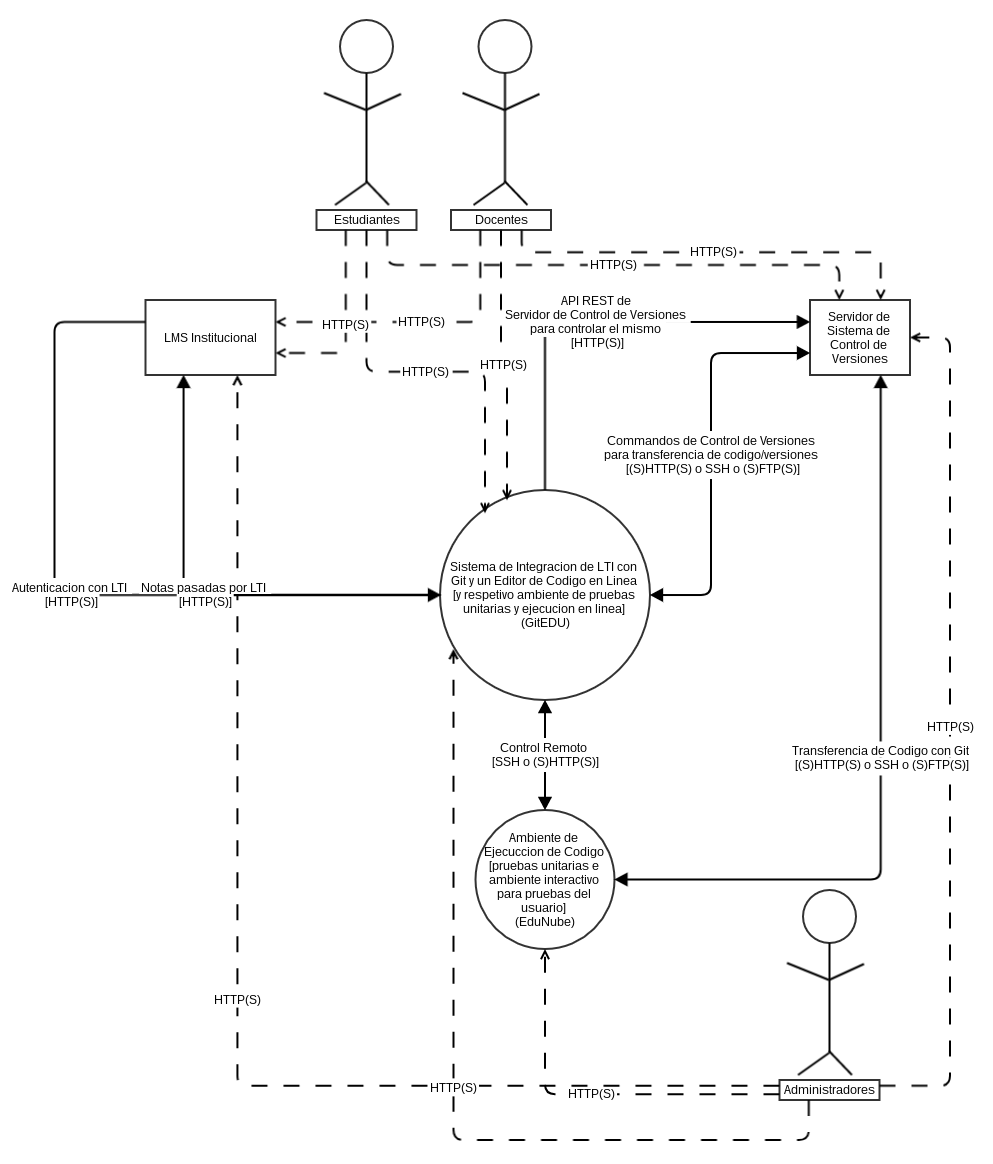
\includegraphics[width=1.7\textwidth]{Figures/contexto.png}
  \end{center}
  \caption{Diagrama de Contexto para GitEdu y EduNube.}
  \label{context}
\end{figure}

\end{landscape}

El diagrama de contexto visualizado en la figura \ref{context} demuestra la relación entre los tres clases de usuarios, sistemas existentes, los sistemas que se plantea desarrollar y los protocolos de interacción entre sistemas distintas y también entre humanos y sistemas.

Los tres tipos de usuarios que se considera para el sistema son administradores, quienes administran y mantienen todo el sistema en su ambiente de despliegue, docentes, quienes generan contenido didactica para sus estudiantes y califican los mismos motivo por el cual que tienen acceso a los LMS, el sistema de editar codigo (que les permite generar nuevas tareas / exámenes / pruebas / talleres para sus estudiantes y ver el progreso y calificaciones de los mismos) y el sistema de control de versiones (donde puede ver y bajar codigo que escriben estudiantes y ver a un nivel más profundo el historial y evolución del mismo), y estudiantes, quienes tengan acceso a los mismos tres sistemas de los docentes. Los estudiantes acceden al LMS donde vean los tareas / exámenes / pruebas / talleres nuevos que hay y al abrirlos se les lleva, identifica y autentica el sistema de editar código en línea mediante LTI. Los estudiantes realizan sus obligaciones de código, mientras que los mismos se respaldan de forma automática en un servidor de control de versiones independiente de tal forma que se lo puede revisar tanto los estudiantes involucrados como su docente a futuro. Aquello control adicional podría llegar a ser una evidencia importante para la resolución de conflictos entre estudiantes y/o docentes a futuro.

El sistema de editar codigo, apartir de aqui conocido simplemente bajo el nombre GitEDU, controla remotamente por medio de comandos, mediante posiblemente una mezcla de protocolos (SSH, HTTP sobre SSH [SHTTP] y HTTPS), dependiendo de cómo se da el caso, un sistema de ejecucion de código, conocido a partir de aquí en adelante como EduNube, para señalar acciones que debe tomar el segundo y/o datos que necesita sincronizar con la primera. Al mismo tiempo, GitEDU comunica con el servidor de control de versiones mediante su API externa (una API REST) sobre HTTP o HTTPS para controlar el mismo y prepararle para flujos continuos de código editado que puede viajar por una variedad de protocolos como SHTTP, HTTPS, HTTP, SFTP, FTP o FTPS como requiere la situación y ambiente de despliegue. Siempre y cuando EduNube requiere de codigo de algun usuario para realizar una calificación o algún otro tipo de interacción con un usuario que requiere probar el mismo, primero se procede a descargar el código involucrado desde el servidor de control de versiones sobre uno de los protocolos mencionado previamente para el mismo. En base a la naturaleza de las operaciones que está haciendo, comunica sus resultados con GitEDU para que puede manejar las mismas de la forma adecuada. En el caso de notas, GitEDU se encarga de sincronizar las mismas con los LMS institucionales con los cuales está integrado mediante el protocolo LTI.

\subsubsection{GitEdu}

% figure
\begin{figure}
  \begin{center}
    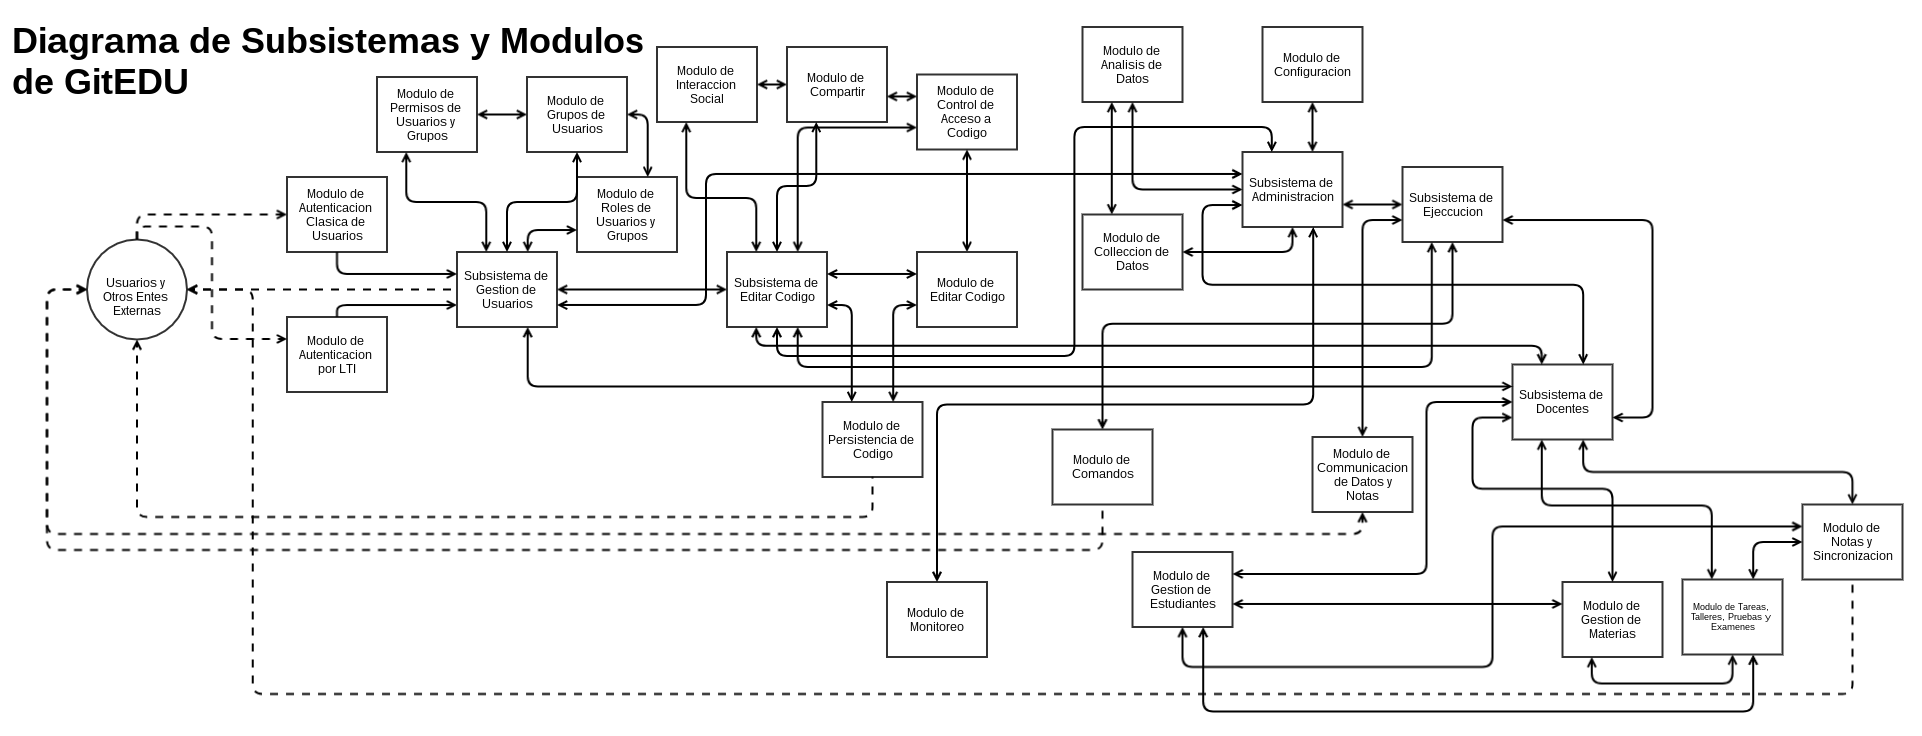
\includegraphics[width=0.75\textwidth]{Figures/mod_ge.png}
  \end{center}
  \caption{Diagrama de Subsistemas y Modulos de GitEdu.}
  \label{mod_ge}
\end{figure}

La figura \ref{mod_ge} presenta todos los componentes en forma de subsistemas y módulos que forman parte del diseño propuesta para el sistema GitEdu.

\paragraph{Subsistema de Gestión de Usuarios}
El subsistema de gestión de usuarios de encarga de temas de seguridad y acceso por usuarios a varios componentes de la aplicación. Para lo mismo autentica usuarios mediante dos módulos (uno clásico y el otro mediante el protocolo LTI) y lleva un sistema de permisos orientado a usuarios, grupos y roles.

\subparagraph{Módulo de Autenticación Clásica de Usuarios}
El módulo de autenticación clásica de usuarios permite que los usuarios finales pueden iniciarse session mediante un usuario y contraseña.

\subparagraph{Módulo de Autenticación por LTI}
El módulo de autenticación por LTI permite que usuarios finales puede iniciar su sesión mediante una sesión existente en algún sistema externa que soporta LTI.

\subparagraph{Módulo de Grupos de Usuarios}
El módulo de grupos de usuarios permite definir grupos específicos de usuarios cuyo membresía les cambia el nivel y naturaleza del acceso que tengan a la aplicación.

\subparagraph{Módulo de Permisos de Usuarios y Grupos}
El módulo de permisos de usuarios y grupos define la naturaleza de acceso que tengan usuarios autorizados y los grupos a los cuales pertenecen dentro de la aplicación.

\subparagraph{Módulo de Roles de Usuarios y Grupos}
El módulo de roles de usuarios y grupos define las responsabilidades de varios grupos de usuarios y usuarios específicos y en base a los mismos les asigna permisos adecuados tanto para proteger la aplicación contra uso y accesos indebidos y al mismo tiempo permitir a los usuarios poder realizar sus actividades normalmente sin impedimentos.

\paragraph{Subsistema de Editar Código}
El subsistema de editar codigo forma el núcleo de la funcionalidad del sistema GitEdu. Eso lo realiza a través de funcionalidades de editar codigo, persistirlo y permitir la interacción adecuada y social entre usuarios.

\subparagraph{Modulo de Editar Codigo}
El módulo de editar código en línea ofrece funcionalidades básicas de un editor de código (IDE) en línea.

\subparagraph{Modulo de Persistencia de Codigo}
El módulo de persistencia de código persiste codigo versionado en servidores de control de versiones externas que usuarios escriben y editan, y al momento de necesitar abrir un código previo, recupera el mismo de los servidores de control de versiones externas para que puede seguir editando lo mismo.

\subparagraph{Módulo de Control de Acceso de Código}
El módulo de control de acceso de código permite a usuarios definir y modificar los permisos que tiene su código para controlar la naturaleza del acceso que tienen otros usuarios, grupos y roles.

\subparagraph{Modulo de Compartir}
El módulo de compartir permite compartir el acceso al código con otros usuarios y grupos.

\subparagraph{Módulo de Interacción Social}
El módulo de interacción social permite que usuarios pueden interactuar en tiempo real mientras que editan juntos el código.

\paragraph{Subsistema de Docentes}
El subsistema de docentes ofrece muchas de las funcionalidades que requieren los docentes para llevar exitosamente su materia de programación. Estas funcionalidades incluyen gestión de estudiantes, materias y notas. La gestión de materias y notas también involucra un gestión y calificación de talleres, deberes, pruebas y exámenes. Además por el hecho de que se genera nuevas notas y calificaciones a través de GitEdu, también se encarga de sincronizar notas con otras sistemas externas como los LMS a través de LTI.

\subparagraph{Modulo de Gestion de Estudiantes}
El módulo de gestión de estudiantes permite que docentes pueden ver notas de un estudiante suyo. Además estudiantes pueden revisar sus notas y tanto administradores como docentes pueden asignar estudiantes a aulas o cambiar o eliminar asignaciones previas.

\subparagraph{Módulo de Gestión de Materias}
El módulo de gestión de materias permite a docentes y administradores ver estadísticas de una materia, la creación de grupos de estudiantes dentro de una materia (por ejemplo para un proyecto grupal) tanto por parte de un docente o por parte de un estudiante, modificar grupos de estudiantes (por ejemplo botar un integrante), y asignar talleres, deberes, pruebas o exámenes a un estudiante, grupo o materia. Además dentro de la gestión de materias, docentes pueden establecer el peso de cada taller, deber, prueba y examen para en base a ello calcular los promedio de un estudiante.

\subparagraph{Módulo de Talleres, Deberes, Pruebas y Exámenes}
El módulo de talleres, deberes, pruebas y exámenes permite a docentes definir nuevos talleres, deberes, pruebas, exámenes, etc y los criterios de evaluación de los mismos. Involucrado en eso son pruebas unitarias (si desee calificación automatizada) y documentación que explica lo que hay que hacer al estudiante.

\subparagraph{Módulo de Notas y Sincronización}
El módulo de notas y sincronización gestiona las notas que mantiene GitEdu y se encarga de sincronizar cambios en las mismas. Aunque realiza este trabajo por detrás normalmente, también proporciona una interfaz gráfica para interacción con los docentes respectivos y adecuados. Además por el tema de seguridad y integridad de las notas, se lleva las mismas versionado y con un registro preciso de cuando fueron modificados y por quien.

\paragraph{Subsistema de Ejecución de Código}
El subsistema de ejecución de código se encarga de comunicar con el sistema externa EduNube con un fin de aprovechar las funcionalidades del mismo y proveer funcionalidades de ejecución en línea, aplicación de pruebas unitarias y calificación automática de código sin exponer el sistema EduNube a usuarios finales. Para aumentar la seguridad que logra llevar EduNube, GitEdu communica con lo mismo a través de canales seguros como HTTPS y SSH utilizando métodos de autenticación orientados a una schema de llaves públicas y privadas (criptografía asimétrica) para asegurarse de la identidad de ambos previo al envío de comandos y comunicación de datos y notas.

\subparagraph{Modulo de Comandos}
El módulo de comandos se encarga de controlar el sistema de EduNube a través de su API externa para indicar al mismo cuando debe bajar, ejecutar o calificar algún código.

\subparagraph{Módulo de Comunicación de Datos y Notas}
El módulo de comunicación de datos y notas permite la sincronización de los mismos cuando sea necesario entre EduNube y GitEdu.

\paragraph{Subsistema de Administración}
El subsistema de administración ayuda a administradores de GitEdu recolectar datos acerca del uso del mismo y analizar lo datos en adición a ser capaces de configurar y monitorear el rendimiento del sistema.

\subparagraph{Módulo de Configuración}
El módulo de configuración permite la configuración en tiempo real del sistema GitEdu, por ejemplo conexiones con sistemas externas y gestión de usuarios.

\subparagraph{Modulo de Monitoreo}
El módulo de monitoreo permite ver en tiempo real el consumo del sistema.

\subparagraph{Módulo de Recolección de Datos}
El módulo de recolección de datos lleva un registro continuo del uso del sistema para su revisión y análisis por parte de operadores humanos después tanto para temas de auditoría como toma de decisiones estratégicas.

\subparagraph{Módulo de Análisis de Datos}
El módulo de análisis de datos proporciona las herramientas necesarias para que un operador humano puede interpretar los mismos y sacar sus conclusiones.

\subsubsection{EduNube}

% figure
\begin{figure}
  \begin{center}
    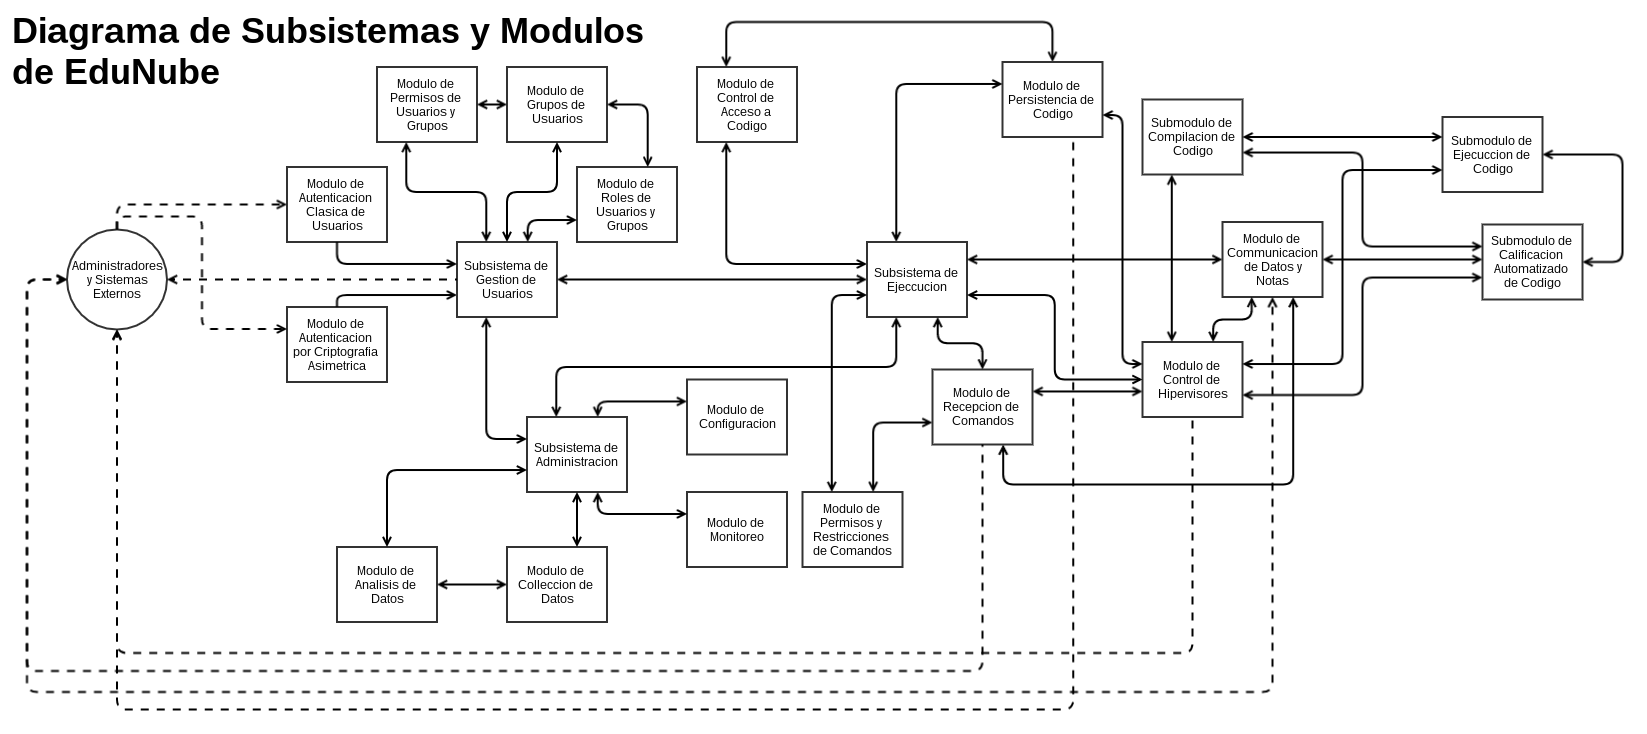
\includegraphics[width=0.75\textwidth]{Figures/mod_en.png}
  \end{center}
  \caption{Diagrama de Subsistemas y Modulos de EduNube.}
  \label{mod_en}
\end{figure}

La figura \ref{mod_en} presenta todos los componentes en forma de subsistemas y módulos que forman parte del diseño propuesta para el sistema EduNube.

\paragraph{Subsistema de Gestión de Usuarios}
El subsistema de gestión de usuarios de encarga de temas de seguridad y acceso indirecto por usuarios (a través de GitEdu) y acceso directo por parte de administradores a varios componentes de la aplicación. Para lo mismo autentica usuarios mediante dos módulos (uno clásico solo para administración del mismo y el otro mediante llaves públicas/privadas [criptografía asimétrica] para aplicaciones externas) y lleva un sistema de permisos orientado a usuarios, grupos y roles.

\subparagraph{Módulo de Autenticación Clásica de Usuarios}
El módulo de autenticación clásica de usuarios permite que administradores pueden iniciarse sesión mediante un usuario y contraseña.

\subparagraph{Módulo de Autenticación por Criptografía Asimétrica}
El módulo de autenticación por criptografía asimétrica permite que usuarios finales, a través de GitEdu puede iniciarse sesión mediante para la ejecución controlada y remoto de comandos y código.

\subparagraph{Módulo de Grupos de Usuarios}
El módulo de grupos de usuarios permite definir grupos específicos de usuarios cuyo membresía les cambia el nivel y naturaleza del acceso que tengan a la aplicación.

\subparagraph{Módulo de Permisos de Usuarios y Grupos}
El módulo de permisos de usuarios y grupos define la naturaleza de acceso que tengan usuarios autorizados y los grupos a los cuales pertenecen dentro de la aplicación.

\subparagraph{Módulo de Roles de Usuarios y Grupos}
El módulo de roles de usuarios y grupos define las responsabilidades de varios grupos de usuarios y usuarios específicos y en base a los mismos les asigna permisos adecuados tanto para proteger la aplicación contra uso y accesos indebidos y al mismo tiempo permitir a los usuarios poder realizar sus actividades normalmente sin impedimentos.

\paragraph{Subsistema de Ejecución}
El subsistema de ejecución de código se encarga de recibir y procesar  comandos del sistema externa GitEdu con un fin de aprovechar los hipervisores que tiene a su cargo y proveer funcionalidades de ejecución en línea, aplicación de pruebas unitarias y calificación automática de código sin exponer dichos hipervisores a usuarios finales. Para aumentar la seguridad que logra llevar EduNube, GitEdu communica con lo mismo a través de canales seguros como HTTPS y SSH utilizando métodos de autenticación orientados a una schema de llaves públicas y privadas (criptografía asimétrica) para asegurarse de la identidad de ambos previo al envío de comandos y comunicación de datos y notas.

\subparagraph{Módulo de Recepción de Comandos}
El módulo de recepción de comandos se encarga de recibir comandos externos enviados a través del API externa que provee para que otras aplicaciones pueden indicar al mismo cuando debe bajar, ejecutar o calificar algún código.

\subparagraph{Módulo de Permisos y Restricciones de Comandos}
El módulo de permisos y restricciones de comandos se encarga de limitar o permitir comandos externos recibidos por el sistema EduNube. Se basa en políticas establecidos previamente que definen los horarios de trabajo de ciertos procesos y dependencias de los mismos (por ejemplo no se debe calificar los exámenes de un parallelo hasta que todos terminan). Junto al modulo de control de acceso a codigo, eso permite a docentes y administradores tener control refinado sobre cuando y que está permitido hacer usuarios que están usando EduNube a través de GitEdu.

\subparagraph{Módulo de Control de Hipervisores}
El módulo de control de hipervisores se encarga de cumplir con la funcionalidades críticos del sistema EduNube de compilar, ejecutar y calificar código. Esto lo hace a través de tres respectivos submódulos para cada fase. De manera más general, este módulo también controla hipervisores conectados al sistema EduNube con un fin de poder realizar las operaciones listados previamente.
\begin{description}
	\item[Submódulo de Compilación de Código]
	El submódulo de compilación de código se encarga de compilar codigo que se le entrega en base a procedimientos que define el profesor anteriormente y reporta resultados del mismo, sea exitosa o sea errores de compilación. Para la implementación del mismo submódulo, se aprovecha de las máquinas virtuales que provee el hipervisor con un fin de realizar la compilación en un ambiente controlado y aislado.
    \item[Submódulo de Ejecución de Código]
	El submódulo de ejecucion de codigo recibe de entradas codigo compilado y comandos que se desee ejecutar en el ambiente de ejecución y pruebas con un fin de proveer, a través de las máquinas virtuales controladas y aisladas, un ambiente interactivo donde estudiantes, tanto estudiantes como docentes pueden trabajar de una forma interactiva con código desarrollado dentro de la plataforma.
    \item[Submódulo de Calificación Automatizado de Código]
	El submódulo de calificación automatizado de código se basa en pruebas unitarias escritas previamente por un docente y que van contra la funcionalidad que se pide en el código de los estudiantes con un fin de calificar el código de una forma autónoma. Una vez que termina de calificar un código, reporta los resultados a gestores de los mismos.
\end{description}

\subparagraph{Módulo de Persistencia de Código}
El módulo de persistencia de código recupere codigo versionado en servidores de control de versiones externas que usuarios han escrito y editado con un fin de permitir la compilación, ejecución y calificación del mismo dentro del sistema EduNube.

\subparagraph{Módulo de Control de Acceso a Código}
El módulo de control de acceso a codigo se encarga de restringir y permitir en base a reglas las operaciones de compilación, ejecución y calificación automatizada de códigos que usuarios editan. De la misma forma permite definir flujos de trabajo y dependencias para el procesamiento de proyectos en adición a establecer horarios y restricciones de procesamiento para los mismos.

\subparagraph{Módulo de Comunicación de Datos y Notas}
El módulo de comunicación de datos y notas permite la sincronización de los mismos cuando sea necesario entre EduNube y GitEdu.

\paragraph{Subsistema de Administración}
El subsistema de administración ayuda a administradores de EduNube recolectar datos acerca del uso del mismo y analizar lo datos en adición a ser capaces de configurar y monitorear el rendimiento del sistema.

\subparagraph{Módulo de Configuración}
El módulo de configuración permite la configuración en tiempo real del sistema EduNube, por ejemplo conexiones con sistemas externas, gestión de llaves públicas y privadas, y gestión de usuarios.

\subparagraph{Modulo de Monitoreo}
El módulo de monitoreo permite ver en tiempo real el consumo del sistema y sus hipervisores respectivos.

\subparagraph{Módulo de Recolección de Datos}
El módulo de recolección de datos lleva un registro continuo del uso del sistema para su revisión y análisis por parte de operadores humanos después tanto para temas de auditoría como toma de decisiones estratégicas.

\subparagraph{Módulo de Análisis de Datos}
El módulo de análisis de datos proporciona las herramientas necesarias para que un operador humano puede interpretar los mismos y sacar sus conclusiones.

\subsubsection{Ventajas del Diseño de Sistemas, Subsistemas y Módulos}
La ventaja de un diseño orientado a módulos como se lo presenta aquí es la división de funcionalidad para ayudar en la extensibilidad y mantenibilidad de los sistemas al largo plazo. Por ejemplo este diseño permite agregar funcionalidad adicional a futuro como autenticación por otros medios (por ejemplo LDAP) o la integración de mecanismos anti-plagio. Esta propiedad puede dar una vida útil mayor a los sistemas desarrolladas porque muchas veces no se conoce todo lo que puede requerir un software a futuro para el diseño e implementación inicial. A continuación se presenta la arquitectura de estos dos sistemas, tanto GitEdu como su ambiente de ejecución de código virtualizado, EduNube.

\subsection{Arquitectura}

% figure
\begin{figure}
  \begin{center}
    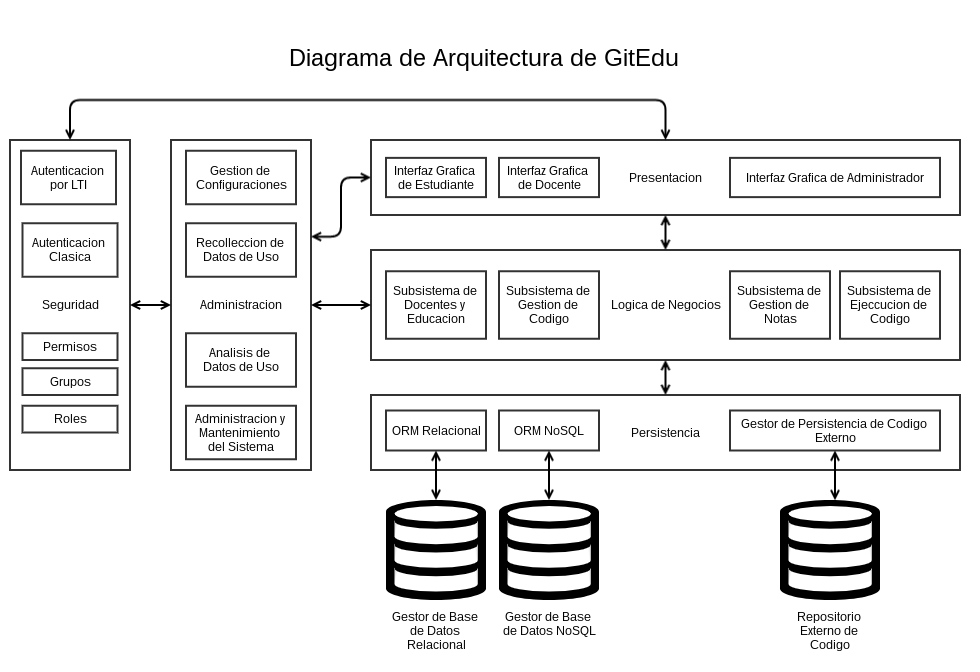
\includegraphics[width=0.75\textwidth]{Figures/arq_ge.png}
  \end{center}
  \caption{Diagrama de arquitectura para el sistema GitEdu.}
  \label{arq_ge}
\end{figure}

Como se puede observar en la figura \ref{arq_ge}, a un nivel global, el sistema GitEdu consiste en 5 capas que son:
\begin{itemize}
	\item \textbf{Seguridad} auténtica usuarios y controla el acceso que tiene cada uno de ellos. Esto se realiza con los siguientes componentes:
    \begin{itemize}
    	\item \textbf{Autenticación por LTI} usa interfaces LTI de aplicaciones externas como LMS institucionales para autenticar usuarios.
		\item \textbf{Autenticación Clásica} permite el login (autenticación) de usuarios mediante la forma clásica de un usuario y contraseña.
		\item \textbf{Permisos} permite otorgar o revocar partes específicas del sistema a usuarios específicos. Ejemplos de permisos podrían ser acceso a la administración de una materia, por ejemplo el control que se da a un docente o grupo de docentes sobre una materia.
		\item \textbf{Grupos} permite aplicar el sistema de permisos a grupos de usuarios creados bajo la discreción de usuarios suficiente privilegiados dentro del sistema. Ejemplos de grupos podrían ser miembros de una cierta materia o tipo de materia, por ejemplo ''Base de Datos''.
		\item \textbf{Roles} permite definir usuarios por su propósito del sistema con un fin de aplicarles un conjunto global de permisos asociados por el tipo de usuario es. Ejemplos de roles podrían ser Estudiante, Docente y Administrador.
    \end{itemize}
    \item \textbf{Administración} permite la administración, mantenimiento y recolección de datos por usuarios dentro del sistema. Para cumplir con estas responsabilidades se divide en:
    \begin{itemize}
    	\item \textbf{Subsistema de Gestión de Configuraciones} que permite a administradores cambiar de forma rapida y facil las configuraciones internas del sistema.
        \item \textbf{Subsistema de Recolección de Datos de Uso} que collecta automáticamente datos del uso del sistema.
        \item \textbf{Subsistema de Análisis de Datos de Uso} que permite a administradores visualizar y analizar los datos que ha recolectado el Subsistema de Recolección de Datos de Uso.
        \item \textbf{Subsistema de Administración y Mantenimiento} que permite a administradores ver en tiempo real y también registros históricos de consumo de recursos. Este subsistema también proporciona a administradores las herramientas que necesita para gestionar y controlar problemas como usuarios maliciosos, sistemas caídos entre otros problemas detectados.
    \end{itemize}
    \item \textbf{Presentación} que se encarga de presentar interfaces web a varias tipos de usuario, incluyendo:
    \begin{itemize}
    	\item \textbf{Estudiantes}
		\item \textbf{Docentes}
		\item \textbf{Administradores}
    \end{itemize}
    \item \textbf{Lógica de Negocios} que se encarga de llevar a cabo los procesos de negocio por el cual la aplicación tiene propósito. Esto se subdivida en cuatro subsistemas:
    \begin{itemize}
    	\item \textbf{Subsistema de Docentes y Educación} que se lleva a cabo procesos de negocio que tienen que ver con enseñanza y evaluación. Dentro de esta subsistema también se lleva las tareas de administración asociadas con un docente y sus aulas de alumnos.
        \item \textbf{Subsistema de Gestión de Código} lleva el control del código y los procesos asociados en cuanto.
        \item \textbf{Subsistema de Gestión de Notas} maneja los procesos de negocio asociados con la sincronización y auditoría de notas generadas dentro del sistema.
        \item \textbf{Subsistema de Ejecución de Código} que lleva a cabo procesos de negocio que tienen que ver con ejecución arbitraria de código y por lo tanto requiere un cierto nivel de seguridad y aislamiento elevado a través de entornos virtualizados. Dentro de los procesos que se incluyen aquí, hay compilación, ejecución y calificación de código automatizado mediante pruebas unitarias.
    \end{itemize}
    \item \textbf{Persistencia} que se encarga de asegurar que se persisten datos importantes para uso futuro y también la recuperación de los mismos. Esto se subdivide en tres clases de persistencia:
    \begin{itemize}
    	\item Persistencia a través de un \textbf{ORM Relacional} que guarda y recupera datos estructurados de la aplicación en bases de datos relacionales y orienta los mismos datos a objetos dentro de la aplicación para permitir su facil manipulacion.
        \item Persistencia a través de un \textbf{ORM NoSQL} que guarda y recupera datos no estructurados de la aplicación en bases de datos no relacionales y orienta los mismos datos a objetos dentro de la aplicación para permitir su facil manipulacion.
        \item Persistencia de código a través de un \textbf{Gestor de Persistencia de Código Externo} que guarda y recupera codigo de usuarios para su manipulación dentro de la aplicación y persistencia fuera del mismo.
    \end{itemize}
\end{itemize}

% figure
\begin{figure}
  \begin{center}
    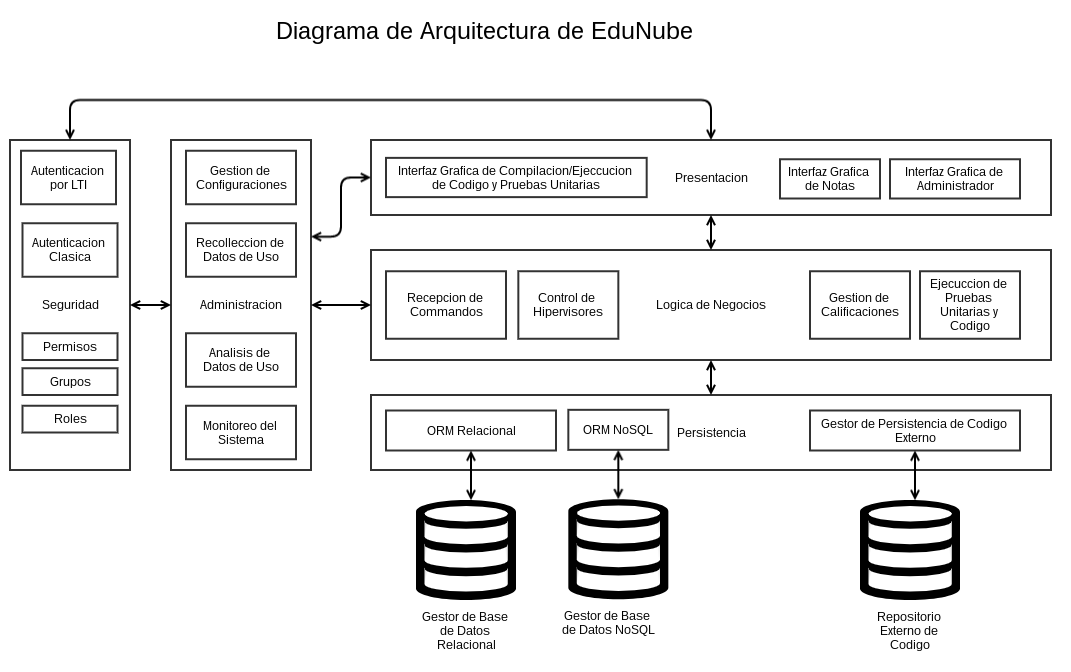
\includegraphics[width=0.75\textwidth]{Figures/arq_en.png}
  \end{center}
  \caption{Diagrama de arquitectura para el sistema EduNube.}
  \label{arq_en}
\end{figure}

Como se puede observar en la figura \ref{arq_en}, a un nivel global, el sistema EduNube consiste en 5 capas que son:
\begin{itemize}
	\item \textbf{Seguridad} auténtica administradores y sistemas externos y controla el acceso que tiene cada uno de ellos. Esto se realiza con los siguientes componentes:
    \begin{itemize}
    	\item \textbf{Autenticación por Criptografía Asimétrica} usa pares de llaves públicas y privadas suficientemente grandes para ser difíciles de falsificar matemáticamente para autenticar sistemas externas.
    	\item \textbf{Autenticación Clásica} permite el login (autenticación) de administradores mediante la forma clásica de un usuario y contraseña.
    	\item \textbf{Permisos} permite otorgar o revocar partes específicas del sistema a usuarios específicos. Ejemplos de permisos podrían ser quien puede crear máquinas virtuales o ver el consumo de recursos del sistema.
    	\item \textbf{Grupos} permite aplicar el sistema de permisos a grupos de usuarios creados bajo la discreción de administradores suficiente privilegiados dentro del sistema. Ejemplos de grupos podrían ser ciertos tipos de usuario que representa algun tipo de estudiante en algún tipo de materia, por ejemplo para la materia de ''Base de Datos''.
    	\item \textbf{Roles} permite definir usuarios por su propósito del sistema con un fin de aplicarles un conjunto global de permisos asociados por el tipo de usuario es. Ejemplos de roles podrían ser Sistema Externa y Administrador.
    \end{itemize}
	\item \textbf{Administración} permite la administración, mantenimiento y recolección de datos por usuarios dentro del sistema. Para cumplir con estas responsabilidades se divide en:
    \begin{itemize}
    	\item \textbf{Subsistema de Gestión de Configuraciones} que permite a administradores cambiar de forma rapida y facil las configuraciones internas del sistema.
    	\item \textbf{Subsistema de Recolección de Datos de Uso} que collecta automáticamente datos del uso del sistema.
    	\item \textbf{Subsistema de Análisis de Datos de Uso} que permite a administradores visualizar y analizar los datos que ha recolectado el Subsistema de Recolección de Datos de Uso.
    	\item \textbf{Subsistema de Monitoreo} que permite a administradores ver en tiempo real y también registros históricos de consumo de recursos. Este subsistema también proporciona a administradores las herramientas que necesita para gestionar y controlar problemas como usuarios maliciosos, sistemas caídos entre otros problemas detectados.
    \end{itemize}
	\item \textbf{Presentación} que se encarga de presentar interfaces web a varias tipos de usuario, incluyendo:
    \begin{itemize}
    	\item \textbf{Compilación/Ejecución de Código y Pruebas Unitarias} proporciona las interfaces gráficas utilizadas durante la compilacion y ejecucion de codigo en adición a la aplicación de pruebas unitarias contra un codigo para ayudar en la calificación del mismo.
        \item \textbf{Notas} permite a docentes y sistemas externos ver las notas asignados a un código.
        \item \textbf{Administradores} proporciona las interfaces gráficas necesarias para ayudar un administrador cumplir con sus responsabilidades de monitoreo, control y mantenimiento del sistema en ambientes de producción.
    \end{itemize}
	\item \textbf{Lógica de Negocios} que se encarga de llevar a cabo los procesos de negocio por el cual la aplicación tiene propósito. Esto se subdivida en cuatro subsistemas:
    \begin{itemize}
    	\item \textbf{Subsistema de Recepción de Comandos} que se lleva a cabo procesos de negocio que tienen que ver con recibir comandos de sistemas externas y procesar las mismas.
        \item \textbf{Subsistema de Control de Hipervisores} lleva el control de los hipervisores conectados y les guía en el proceso de virtualizar y ejecutar código dentro de máquinas virtuales de los mismos hipervisores.
        \item \textbf{Subsistema de Calificaciones} maneja los procesos de negocio asociados con la calificación, sincronización y auditoría de notas generadas dentro del sistema.
        \item \textbf{Subsistema de Ejecución de Código y Pruebas Unitarias} que lleva a cabo procesos de negocio que tienen que ver con ejecución arbitraria de código en entornos virtualizados. Dentro de los procesos que se incluyen aquí, hay compilación, ejecución y calificación de código automatizado mediante pruebas unitarias.
    \end{itemize}
	\item \textbf{Persistencia} que se encarga de asegurar que se persisten datos importantes para uso futuro y también la recuperación de los mismos. Esto se subdivide en tres clases de persistencia:
    \begin{itemize}
    	\item Persistencia a través de un \textbf{ORM Relacional} que guarda y recupera datos estructurados de la aplicación en bases de datos relacionales y orienta los mismos datos a objetos dentro de la aplicación para permitir su facil manipulacion.
		\item Persistencia a través de un \textbf{ORM NoSQL} que guarda y recupera datos no estructurados de la aplicación en bases de datos no relacionales y orienta los mismos datos a objetos dentro de la aplicación para permitir su facil manipulacion.
		\item Persistencia de código a través de un \textbf{Gestor de Persistencia de Código Externo} que guarda y recupera codigo de usuarios para su manipulación dentro de la aplicación y persistencia fuera del mismo.
    \end{itemize}
\end{itemize}

\subsubsection{Ventajas del Diseño Arquitectónico}
Se ha considerado para ambos sistemas una arquitectura de n-capas debido a su capacidad de escalabilidad sobre varios niveles físicos. Además la separación lógica entre capas permite mayor mantenibilidad al largo plazo donde solo se necesitan reemplazar los componentes que requieren cambios en lugar de todo el sistema. El nivel de aislamiento entre estas mismas capas brinde mejor seguridad contra usuarios externos sean maliciosos o que quieren dar mal uso (un uso inadecuado) al sistema. A continuación se presenta la arquitectura de despliegue propuesta dentro de este trabajo de titulación.

\subsection{Despliegue}

% figure
\begin{figure}
  \begin{center}
    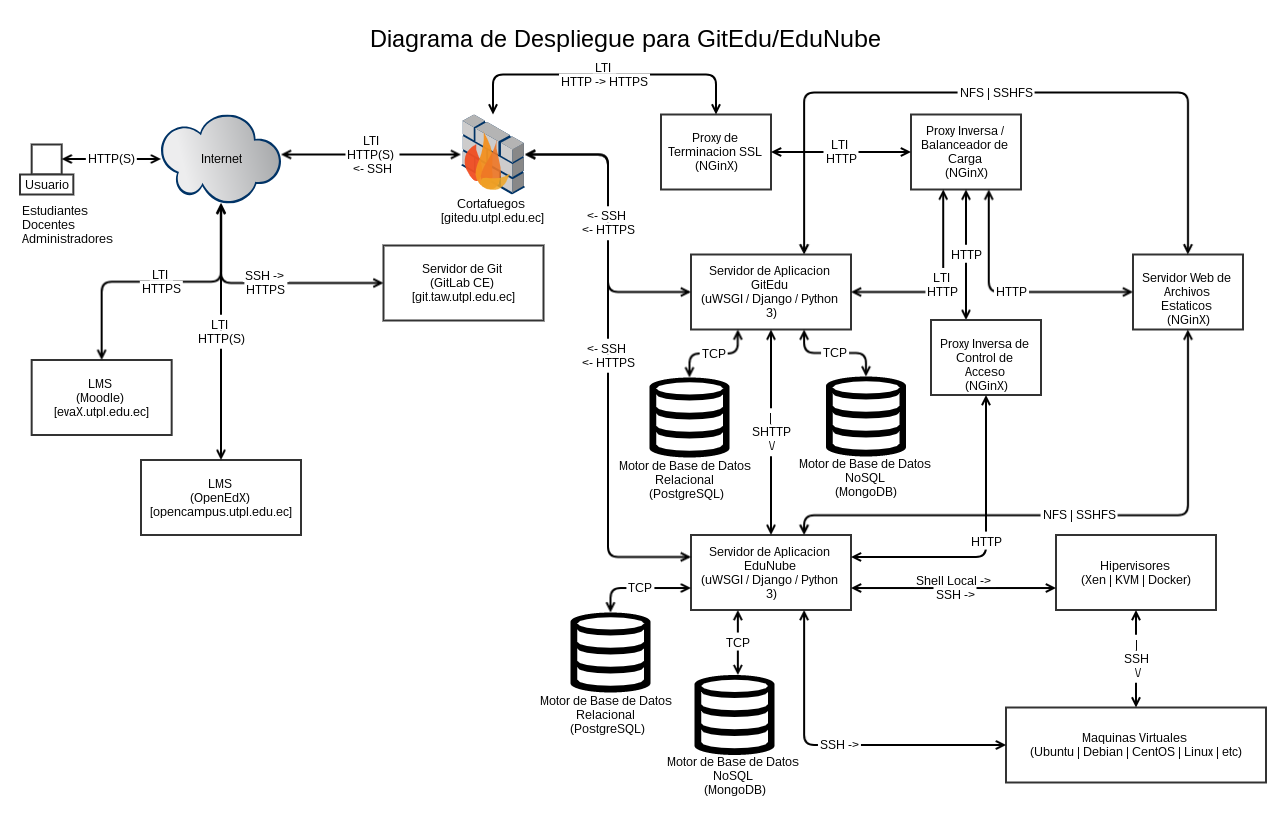
\includegraphics[width=0.75\textwidth]{Figures/desp_ge_en.png}
  \end{center}
  \caption{Diagrama de Despliegue para los sistemas GitEdu y EduNube.}
  \label{desp_ge_en}
\end{figure}

Como se puede observar en la figura \ref{desp_ge_en}, el despliegue del sistema GitEdu junto al sistema EduNube, consiste en dos redes, una externa que contiene los usuarios finales (Estudiantes, Docentes, Administradores) en adición a sistemas externas como los dos LMS institucionales (Moodle y OpenEdX) y el servidor de Git (GitLab Community Edition), mientras que la red interna contiene las varias componentes que forman el conjunto de sistemas:
\begin{itemize}
	\item \textbf{Cortafuegos} divide la red interna de la red externa y permite únicamente que pasa tráfico HTTP y HTTPS de manera bidireccional (con posibilidad de llamadas LTI sobre estos protocolos) y la salida de SSH al servidor de Git (para ofrecer mayor seguridad que transferencias sobre HTTP(S)).
    \item \textbf{Proxy de Terminación SSL} accepta HTTP y HTTPS, pero para asegurar la seguridad de usuarios finales y aplicaciones externas redirecciona toda uso del protocolo HTTP a HTTPS. Además descifra conexiones HTTPS entrantes para manejarlos por HTTP dentro de la red interna (reduciendo la carga en otros servidores sin abandonar seguridad en la red externa) y cifra conexiones salientes. Se utiliza NGinX por su bajo consumo de recursos en comparación con sus competidores como Apache.
    \item \textbf{Proxy Inversa / Balanceador de Carga} accepta todo el tráfico HTTPS (ahora por el protocolo HTTP dentro de la red interna) entrante y elige en base a la ruta cual servidor se lo puede responder. A futuro este componente permite que se puede escalar el sistema en lo que permite dividir tráfico entre varios servidores del mismo tipo (por ejemplo dos servidores de aplicación: GitEdu1 y GitEdu2). Se considera que NGinX es la solución más óptima para realizar este rol.
    \item \textbf{Servidor Web de Archivos Estáticos} se responsabiliza por peticiones de archivos estáticos que no conviene enviar a los servidores de aplicación (quienes los procesaría con mayor lentitud). Estos mismos tienen una conexión NFS o SSHFS con los mismos servidores de aplicación para que estos sean capaces de actualizar remotamente los archivos estáticos en caso de que los mismos cambien (por ejemplo cuando un usuario actualiza su foto de perfil). Estudios de rendimiento demuestran que NGinX cumple este rol de ser servidor web de archivos estáticos mejor que Apache.
    \item \textbf{Servidor de Aplicación ''GitEdu''} se aloja el sistema GitEdu, desarrollado bajo el marco Django y el lenguaje de programación Python (version 3.x). Comunica con el servidor externo de Git sobre SSH y dispone tanto de un base de datos relacional como uno no relacional para persistir los distintos tipos de datos que tiene que manejar. Se conecta directamente al Servidor de Aplicación “EduNube” mediante SHTTP (HTTP sobre un túnel SSH) utilizando un par de llaves (pública y privada) como schéma de criptografía asimétrica. Se considera uWSGI como mejor servidor de aplicación para el sistema debido a que, a diferencia de su competencia (Gunicorn), esta suporta Websockets.
    \item \textbf{Motores de Base de Datos Relacional} se alojan datos estructurados para ambos sistemas, tanto GitEdu como NubeEdu.
    \item \textbf{Motores de Base de Datos NoSQL} se alojan datos no estructurados para ambos sistemas, tanto GitEdu como NubeEdu.
    \item \textbf{Proxy Inversa de Control de Acceso} restringe acceso al servidor de aplicaciones de EduNube cuando se accede al mismo desde la red externa (a través del proxy inversa).
    \item \textbf{Servidor de Aplicación ''EduNube''} se aloja el sistema EduNube, desarrollado bajo el marco Django y el lenguaje de programación Python (version 3.x). Comunica con el servidor externo de Git sobre SSH y dispone tanto de un base de datos relacional como uno no relacional para persistir los distintos tipos de datos que tiene que manejar. Utiliza un shell local (dentro del mismo servidor) para manejo de un hipervisor local o en el caso de un hipervisor remoto, maneja el mismo sobre SSH. Las máquinas virtuales que se levanta el hipervisor, también se los controla con SSH. Se considera uWSGI como mejor servidor de aplicación para el sistema debido a que, a diferencia de su competencia (Gunicorn), esta suporta Websockets.
    \item \textbf{Hipervisores} gestionan máquinas virtuales por parte del sistema EduNube quien le envía comandos por SSH o un shell local. A su vez, controla sus máquinas virtuales mediantes SSH. Como tecnologías de hipervisor se considera Xen, KVM y Docker como buenas opciones para diferentes necesidades. Cada sistema de hipervisores soporta el uso de plantillas para la creación masiva de máquinas virtuales iguales para cada estudiante de una materia.
    \item \textbf{Máquinas Virtuales} ejecutan código de usuarios y reportan los resultados.
\end{itemize}

\subsubsection{Ventajas de la Arquitectura de Despliegue}
De la misma moda como el diseño de sistemas, subsistemas y módulos en adición al diseño arquitectónico, el diseño de arquitectura de despliegue está orientado a extensibilidad a través de modularidad, mantenibilidad por la naturaleza de sus capas y módulos, además de escalabilidad y seguridad mantenido a través de mecanismos de aislamiento de componentes que sean libres de escalar independientemente entre ellos, la arquitectura de despliegue se orienta a los mismos principios.

La separación de deberes dentro del sistema permite que cada servicio dentro de la arquitectura de despliegue se puede dedicar a hacer bien su parte de la manera más eficiente posible sin responsabilidades que no puede sostener de forma inadecuada, algo importante para empezar a poder garantizar rendimiento óptimo del sistema. El uso de un cortafuegos y varias proxies inversas adelantes de cada sistema también ayuda aislar las mismas del mundo externo a un nivel de protocolos reduce los superficies de ataque contra las mismas para ofrecer seguridad sin sacrificar rendimiento de una manera similar al punto anterior de separación de trabajo en roles y asignación al actor más adecuado para el mismo.

Este mismo uso de trabajadores, especializado cada uno en sus responsabilidades y posible carga de trabajo también sigue ofreciendo escalabilidad a futuro. Esto se realiza con comunicación entre servicios que está sobre protocolos de red para que las mismas o pueden estar en un solo recurso (sea servidor fisica o virtual) o en varios apartados lo cual permite a futuro la asignación de recursos físicos o virtuales como se lo ve la necesidad. Esta capacidad para escalar se puede ofrecer gracias al hecho de que los servicios semi independientes unos de otros, permitiendo n-capas sobre m-niveles físicos/lógicos.

Donde haya dependencias de, por ejemplo, sistema de ficheros compartidos para dos capas distintas se puede implementar con protocolos que permiten acceso remoto para las operaciones necesarios, en este caso que los servidores de aplicación sean capaces de actualizar los archivos estáticos en el servidor para el mismo (se lo está considerando esta parte con un NFS o SSHFS). Obviamente en el caso de que estén en el mismo servidor, no se da la necesidad de establecer aquello conexión.

En casos donde se considera una necesidad de mayor seguridad en proteger canales de comunicación, se ha considerado que la mejor forma de brindar lo mismo es con tunnels SSH que encapsulan trafico que por si sola ocupa un protocolo adecuado según la necesidad. Por ejemplo para consumir el API de EduNube, GitEdu utiliza HTTP sobre SSH (también conocido como SHTTP). De esta forma se puede aprovechar lo que ya existe y que está comprobada como segura y eficiente (SSH como protocolo, especialmente en su segunda versión, obliga fuertes mecanismos de autenticación y seguridad mientras que al mismo tiempo ofrece menor sacrificio de rendimiento y alta funcionalidad).

A continuación se presenta el alcance del desarrollo, pruebas y despliegue para este trabajo de titulación.

\subsection{Alcance}

Debido al hecho de que se cuenta con tiempo y recursos limitados para realizar y acabar el trabajo de titulación, se considera un alcance limitado en ciertos aspectos con un fin de acabar con los componentes críticos del sistema dentro del tiempo dado.

% figure
\begin{figure}
  \begin{center}
    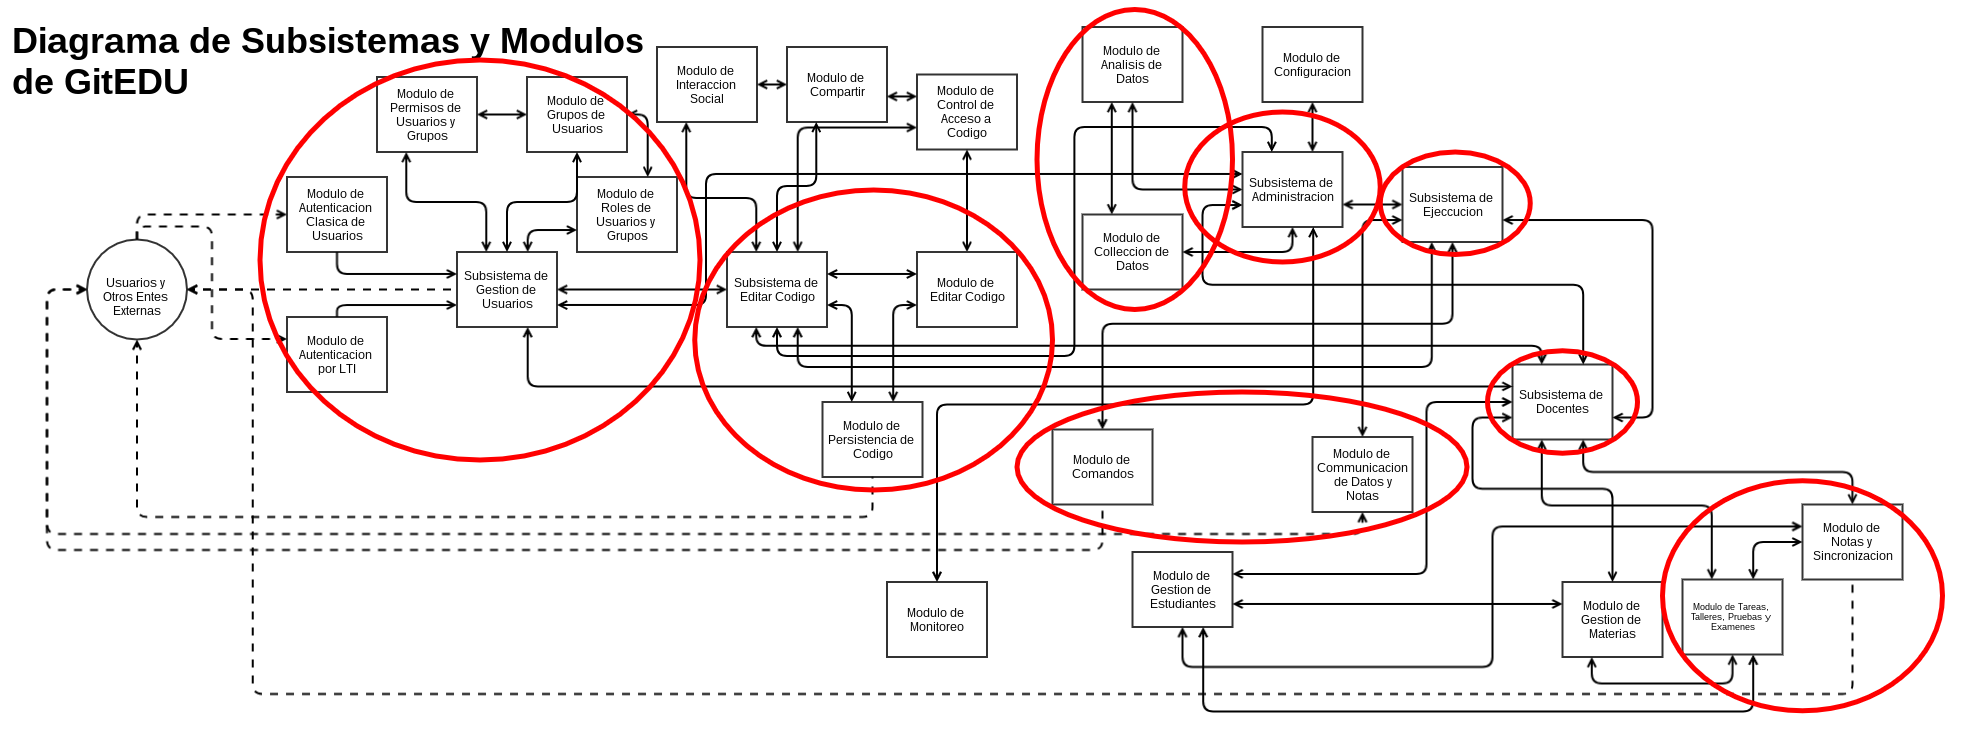
\includegraphics[width=0.75\textwidth]{Figures/alc_mod_ge.png}
  \end{center}
  \caption{Alcance de Módulos para GitEdu.}
  \label{alc_mod_ge}
\end{figure}

Para el sistema GitEdu se considera los siguientes subsistemas y módulos críticos como se puede observar en la figura \ref{alc_mod_ge}:
\begin{itemize}
	\item \textbf{Todo el subsistema de Gestión de Usuarios.} Todos los módulos de este sistema son críticos porque se encargan de cómo los usuarios se autentican contra el mismo y el control de acceso que tienen cada uno. Por lo tanto el subsistema en sí es una parte importante para garantizar seguridad en el sistema final.
    \item \textbf{Parte del subsistema de Editar Código.} El subsistema de editar codigo se considera crítico los módulos tanto de editar como de persistir codigo. El módulo de editar codigo es crítico porque forma la funcionalidad principal de que se trata el sistema mientras que el modulo de persistir codigo viene a ser critico para sincronizar codigo entre los dos sistemas. No se toma en consideración como críticos los módulos de interacción social, compartir codigo ni control de acceso a codigo porque las mismas se tratan de llevar el sistema más allá de su propósito original y son más adecuados para un futuro trabajo.
    \item \textbf{Parte del subsistema de Docentes.} Dentro del subsistema de docentes, se considera crítico un módulo de crear talleres, pruebas y exámenes en adición a un módulo de notas y su sincronización. Entre estos dos se forma el núcleo de funcionalidad que requieren docentes dentro de la versión inicial. Dentro de trabajos futuros, se podría extender esta funcionalidad crítica con temas más administrativas como los módulos de gestión de materias y gestión de estudiantes que por el momento no se los considera como funcionalidades críticas para una primera versión estable, el producto de este trabajo de titulación.
    \item \textbf{Parte del subsistema de Administración.} Dentro del subsistema de administración, solo se considera que los componentes críticos se tratan de colección de datos y el análisis de los mismos debido a que esos dos módulos respectivamente ayudan en la toma de decisiones estratégicas que tienen que ver con la escuela de Ciencias de Computación y Electrónica y el uso del sistema. Los módulos de monitoreo y configuración, aunque podrían ser muy útiles en un ambiente de producción no caen dentro del alcance inicial de este tesis y por lo tanto no se los considera críticos bajo los parámetros del proyecto. De todas formas su implementación podría ser una funcionalidad adicional interesante para un futuro proyecto.
    \item \textbf{Todo el subsistema de Ejecución.} Todos los módulos de este sistema son críticos porque se encargan de la comunicación con el sistema EduNube. El módulo de comandos prepara comandos para ejecutar a través del módulo de comunicación de datos y notas se los envía en adición a conseguir resultados y sincronizar notas y calificaciones generadas por EduNube.
\end{itemize}

% figure
\begin{figure}
  \begin{center}
    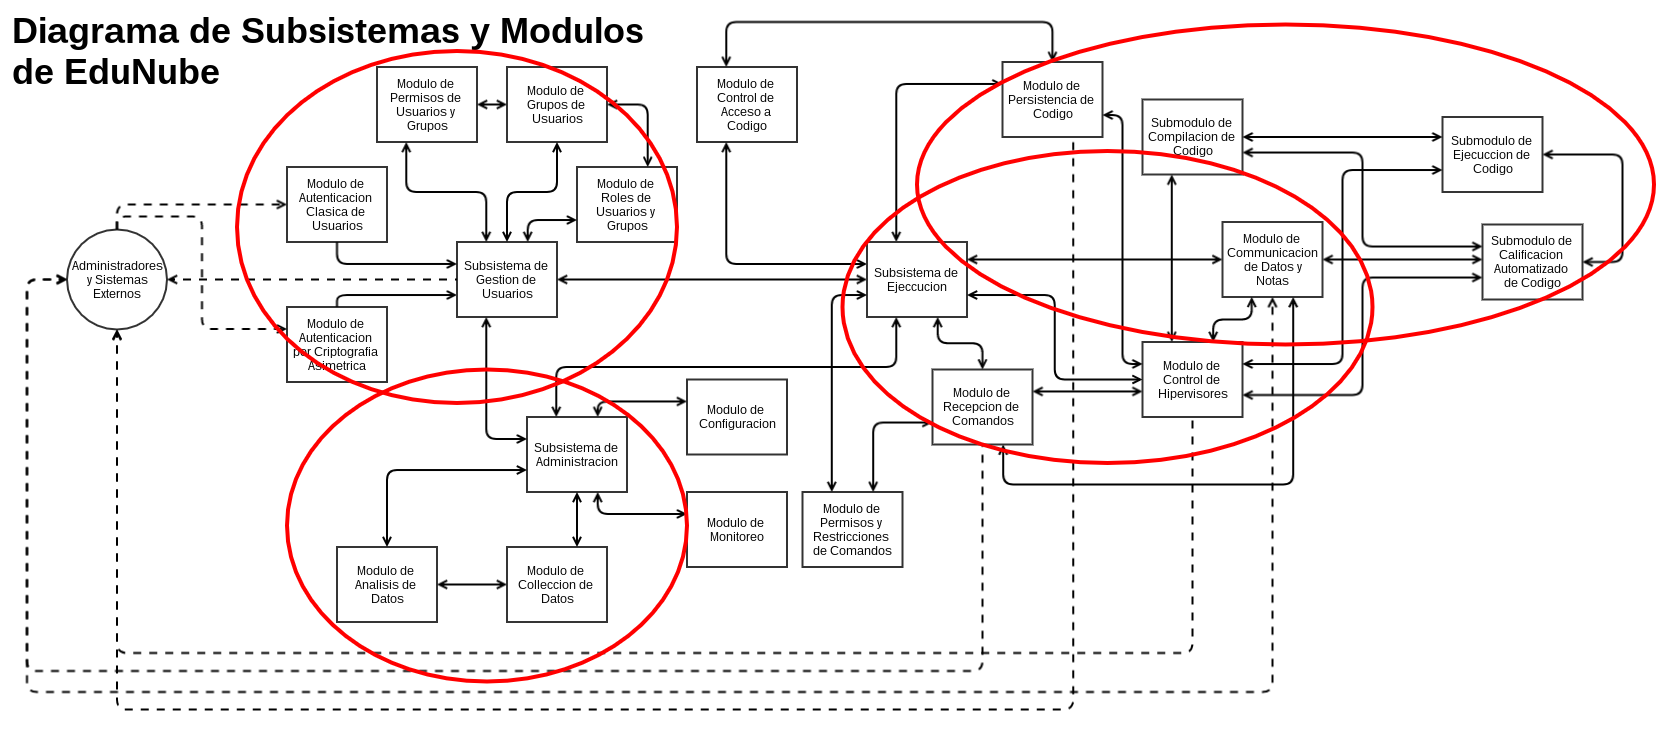
\includegraphics[width=0.75\textwidth]{Figures/alc_mod_en.png}
  \end{center}
  \caption{Alcance de Módulos para EduNube.}
  \label{alc_mod_en}
\end{figure}

Para el sistema EduNube, se considera los siguientes subsistemas y módulos como críticos, de la forma que estan demostradas en la figura \ref{alc_mod_en}:
\begin{itemize}
	\item \textbf{Todo el subsistema de Gestión de Usuarios.} Todos los módulos de este sistema son críticos porque se encargan de cómo los usuarios se autentican contra el mismo y el control de acceso que tienen cada uno. Por lo tanto el subsistema en sí es una parte importante para garantizar seguridad en el sistema final.
	\item \textbf{Parte del subsistema de Ejecución.} Dentro del subsistema de ejecución se consideran críticos los módulos de comandos (para procesar comandos entrantes), de control de hipervisores (para gestionar recursos virtuales), y de persistencia de código (para recuperar código para su compilación, compilación y ejecución).  Además como componentes del módulo de control de hipervisores, se considera crítico los submódulos de compilación de código (para aquellos lenguajes que lo requieren), de ejecución (para ejecutar código), y de calificación automatizado de código (para calificar codigo de estudiantes). Se considera que los módulos de seguridad adicionales dentro de este subsistema no son necesarios por el momento debido al que único sistema que tendrá acceso a esta será la de GitEdu. A futuro, donde más sistemas y servicios empiezan a necesitar consumir el API de EduNube, llegará a ser necesario que tenga aquellos módulos de seguridad para proveer protección adicional.
	\item \textbf{Parte del subsistema de Administración.} Dentro del subsistema de administración, solo se considera que los componentes críticos se tratan de colección de datos y el análisis de los mismos debido a que esos dos módulos respectivamente ayudan en la toma de decisiones estratégicas que tienen que ver con la escuela de Ciencias de Computación y Electrónica y el uso del sistema. Los módulos de monitoreo y configuración, aunque podrían ser muy útiles en un ambiente de producción no caen dentro del alcance inicial de este tesis y por lo tanto no se los considera críticos bajo los parámetros del proyecto. De todas formas su implementación podría ser una funcionalidad adicional interesante para un futuro proyecto.
\end{itemize}

% figure
\begin{figure}
  \begin{center}
    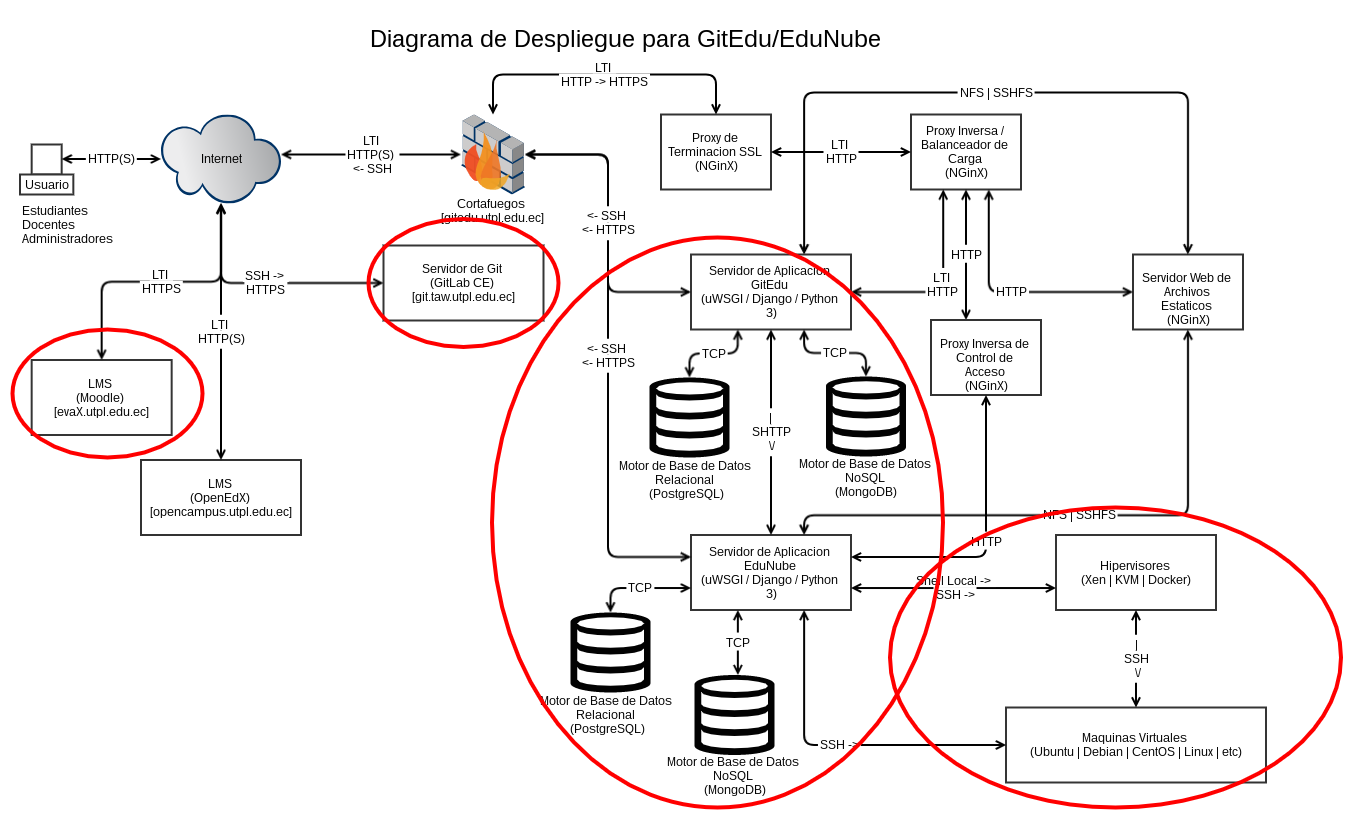
\includegraphics[width=0.75\textwidth]{Figures/alc_desp_ge_en.png}
  \end{center}
  \caption{Alcance de Despliegue.}
  \label{alc_desp_ge_en}
\end{figure}

En cuanto el despliegue (figura \ref{alc_desp_ge_en}), los sistemas externas que se toma en consideración para el alcance son Moodle como LMS, y GitLab Community Edition como servidor de control de versiones. En relación a los ambientes virtuales, solo se considera un hipervisor y un sistema operativo para las máquinas virtuales dentro de la versión final (durante el desarrollo se presenta los candidatos, comparación y selección de los mismos). También se incluye dentro del alcance el desarrollo y despliegue de los dos sistemas GitEdu y EduNube con sus respectivas bases de datos utilizando uWSGI como servidor de aplicación. No se incluye dentro del alcance OpenEdX o ningún otro LMS externa fuera de la mencionada previamente ni las configuraciones del cortafuego y servidores web, estos quedan como responsabilidades institucionales en cuanto como deseen implementar estos partes del despliegue. Lo que se presenta aquí es una sugerencia del autor basado en su experiencia práctica.

% Chapter 4

\chapter{Desarrollo}
\label{capitulo4}

\index{Autenticación LTI|textit} \index{Ejecutar Código} \index{Editar Código} \index{Calificar Código} \index{Persistir Código} \index{Sincronizar Notas por LTI|textit} \index{Controlar Versiones de Código} \index{Recolección de Datos} \index{Toma de Decisiones}
\section{Preparaciones del Ambiente de Desarrollo}
Previo a realizar el desarrollo, es necesario que se prepara el ambiente para la misma con:
\begin{itemize}
  \item un sistema base (Debian Stretch con el Xen Hipervisor)
  \item un servidor local de Git (Git + Gitweb + NGinX),
  \item un servicio para recibir peticiones HTTP y convertirlos en sus respectivos objetos en un repositorio de Git (Git Server HTTP Endpoint)
  \item un LMS \index{LMS} (Moodle),
  \item un servidor de Git (GitLab CE)
  \item un servidor de Virtualización (Docker)
  \item plantillas de maquinas virtuales (en Docker)
\end{itemize}

\subsection{Sistema Base de Desarrollo}

\begin{figure}
	\begin{center}
    	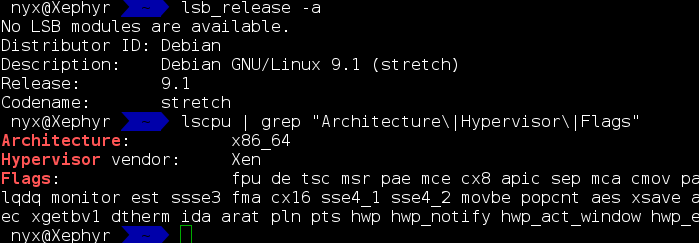
\includegraphics[width=0.75\textwidth]{Figures/sistema-base.png}
    \end{center}
  	\caption{Información del Sistema Base.}
    \label{sistema-base}
\end{figure}

\index{Ejecutar Código}
Como se presenta en la figura \ref{sistema-base}, el sistema base para el desarrollo de este trabajo de titulación utiliza Xen instalado con Debian Stretch (9.1)\footnote{Como el sistema de Dom0} instalado en un LVM con el nombre del grupo de volúmenes ''Xephyr-VG''. Originalmente se tenia planificado trabajar con Debian Jessie (8.x) debido que eso fue la versión estable al momento de instalación pero después se opto por una actualización a la versión beta de Debian en aquello momento (Debian Stretch). En resumen los pasos realizados fueron:
\lstset{language=Bash}
\begin{enumerate}
	\item Instalación Limpia de Debian 8 con un LVM.
    	\begin{description}
    		\item[Volumen Físico:] /dev/sda8 310g 
            \item[Grupo de Volúmenes:] Xephyr-VG 310g
            \item[Volúmenes Lógicos:] Originalmente 4 (se agrega 2 por cada nueva maquina virtual -- uno para su disco y otro para su área de intercambio).
            \begin{description}
            	\item[Xephyr-Dom0] Xephyr-VG 30g
                \item[Xephyr-IMG-Repo] Xephyr-VG 20g
                \item[Xephyr-ISO-Repo] Xephyr-VG 20g
                \item[Xephyr-Swap] Xephyr-VG 4g
            \end{description}
    	\end{description}
    \item Actualizar Instalación de Debian 8.
    	\begin{lstlisting}
	apt update
	apt upgrade
	apt dist-upgrade
	reboot
        \end{lstlisting}
    \item Actualizar Debian 8 a Debian 9.
        \begin{lstlisting}
	sed -i 's/jessie/stretch/g' /etc/apt/sources.list
	apt update
	apt upgrade
	reboot
        \end{lstlisting}
    \item Instalación de Herramientas de Trabajo
        \begin{lstlisting}
	apt install tmux vim zsh
        \end{lstlisting}
    \item Instalación y Configuración de Hipervisor Xen
		\begin{lstlisting}
	apt install xen-hypervisor
	dpkg-divert --divert /etc/grub.d/08_linux_xen \
		--rename /etc/grub.d/20_linux_xen
	update-grub
	cat > /etc/network/interfaces.d/xenbr << EOF

	auto xenbr0
	iface xenbr0 inet static
		address 10.10.10.1
		netmask 255.255.255.0
		bridge_ports wlan0

	#other possibly useful options in a
	#	virtualized environment
		#bridge_stp off		# disable
		#		Spanning Tree Protocol
		#bridge_waitport 0	# no delay
		#		before a port becomes
		#		available
		#bridge_fd 0		# no forwarding
		#		delay

	## configure a (separate) bridge for
	#	the DomUs without giving Dom0 an
	#	IP on it
	#auto xenbr1
	#iface xenbr1 inet manual
	#   bridge_ports eth1

	EOF

	reboot
		\end{lstlisting}
	\item Instalación de Herramientas de Xen
		\begin{lstlisting}
	apt install xen-tools xen-utils
		\end{lstlisting}
    \item Instalación de Herramientas de Desarrollo para Python 3
    	\begin{lstlisting}
	apt install python3 python3-virtualenv python3-pip
    	\end{lstlisting}
        % gitweb fcgiwrap
        % libffi-dev % TODO: Look for other possible dependencies?
    \item Instalación de Servidores
    	\begin{lstlisting}
	apt install nginx-full postgresql mongodb\
    		redis-server
    	\end{lstlisting}
    \item Instalación de IDEs en /opt. Se descargaron los respectivos .tar\textit{.xx} y se los descomprimieron en /opt con un comando similar al siguiente:
    	\begin{lstlisting}
	tar -axvf nombre.tar.xx -C\
    		/opt/ruta/raiz/donde/descomprimir
    	\end{lstlisting}
    \begin{enumerate}
    	\item PyCharm (Community o Professional Edition\footnote{Se ocupo una versión Professional, en parte por su buen suporte para desarrollo en Django) con una licencia estudiantil que actualmente es gratis de solicitar y renovar año tras año con un correo institucional})
        \item DBeaver (Community o Enterprise Edition\footnote{Históricamente siempre han sido gratis ambas versiones con la diferencia siendo que Enterprise Edition no es completamente software libre a diferencia de su versión libre, pero el mismo agrega suporte para bases de datos no relacionales. Se ocupo la versión Enterprise, entre los últimos ofertas gratis antes de que se convierte en un producto de pago, por este mismo motivo de requerir suporte para bases de datos NoSQL como MongoDB y Redis.})
    \end{enumerate}
\end{enumerate}

Estos pasos de instalación se basaron en la guía de instalación de Xen publicado en el wiki del proyecto de Debian \citep{Debian-Wiki-Xen}.

Para dar conexiones hace el exterior a las maquinas virtuales, se necesita activar una regla NAT en el cortafuego IPTables:

\begin{lstlisting}
	iptables -t nat -A POSTROUTING -o wlan0\
    		-j MASQUERADE
\end{lstlisting}

\index{Controlar Versiones de Código} \index{Persistir Código}
\subsubsection{Servidor Local de Git}
Para gestionar versiones de código escrito y facilitar la integración con sistemas externas y el sistema de virtualización, se levanta un servidor sencillo de Git.

Instalar paquetes para un interfaz web sencilla de Git:
\begin{lstlisting}
apt install git gitweb fcgiwrap
\end{lstlisting}

Se crea un usuario del sistema operativo solo para Git:
\begin{lstlisting}
adduser git
\end{lstlisting}

Se autentica como el usuario creado:
\begin{lstlisting}
su - git
\end{lstlisting}

Para tener repositorios ejemplares, se clona algunos repositorios:
\begin{lstlisting}
git clone --bare https://gitlab.com/nishedcob/GitEDU.git repositories/GitEDU.git
git clone --bare https://gitlab.com/ArqAppGrpBravoEarleyVargas/GitEduERP.git repositories/GitEduERP.git
\end{lstlisting}

Entrar al directorio de repositorios y arreglar permisos para permitir git push desde repositorios remotos:
\begin{lstlisting}
cd repositories/
for repo in `ls`; do
	cd $repo;
    pwd;
    chmod -R g+ws .;
    chgrp -R git .;
    git --bare update-server-info;
    cp hooks/post-update.sample hooks/post-update;
    chmod a+x hooks/post-update;
    cd ..;
done
\end{lstlisting}

Después se configura NGinX para trabajar con gitweb:
\begin{lstlisting}
# NGinX Config:
server {
        listen 80;
        listen [::]:80;
        server_name git.localhost;
        root /usr/share/gitweb;
        access_log /var/log/nginx/gitweb.access.log;
        # static repo files for cloning over https
        location ~ ^.*\.git/objects/([0-9a-f]+/[0-9a-f]+|pack/pack-[0-9a-f]+.(pack|idx))$ {
                root /home/git/repositories/;
        }

        # requests that need to go to git-http-backend
        location ~ ^.*\.git/(HEAD|info/refs|objects/info/.*|git-(upload|receive)-pack)$ {
                root /home/git/repositories;

                fastcgi_pass unix:/var/run/fcgiwrap.socket;
                fastcgi_param SCRIPT_FILENAME   /usr/lib/git-core/git-http-backend;
                fastcgi_param PATH_INFO          $uri;
                fastcgi_param GIT_PROJECT_ROOT  /home/git/repositories;
                fastcgi_param GIT_HTTP_EXPORT_ALL "";
                fastcgi_param REMOTE_USER $remote_user;
                include fastcgi_params;
        }

        # send anything else to gitweb if it's not a real file
        try_files $uri @gitweb;
        location @gitweb {
                fastcgi_pass unix:/var/run/fcgiwrap.socket;
                fastcgi_param SCRIPT_FILENAME   /usr/share/gitweb/gitweb.cgi;
                fastcgi_param PATH_INFO          $uri;
                fastcgi_param GITWEB_CONFIG      /etc/gitweb.conf;
                include fastcgi_params;
        }
}
\end{lstlisting}

Además se configura gitweb con la siguiente configuración:
\begin{lstlisting}
# Edit /etc/gitweb.conf
# path to git projects (<project>.git)
#$projectroot = "/var/lib/git";
$projectroot = "/home/git/repositories";
\end{lstlisting}

Prueba de que funciona:
\begin{lstlisting}
git clone http://git.localhost/nishedcob/GitEDU.git GitEDU-test
\end{lstlisting}

\index{Persistir Código} \index{Controlar Versiones de Código}
\subsubsection{Git Server HTTP Endpoint}
Para recibir llamadas HTTP y convertirlos en sus respectivos objetos en un repositorio de Git, se creó un miniservicio que realiza esta tarea, basado en la misma app de autenticación que utiliza EduNube:
\begin{lstlisting}
pipenv --three
pipenv install django six psycopg2 PyJWT bcrypt ipython
pipenv run django-admin startproject GitServerHTTPEndpoint .
# Configurar Base de Datos, Reutilizar authApp de EduNube, migrar la base de datos, Crear un superusuario
rsync -av --progress ~/EduNube/authApp ~/GitServerHTTPEndpoint/
vim GitServerHTTPEndpoint/settings.py
pipenv run python manage.py makemigrations authApp
pipenv run python manage.py migrate
pipenv run python manage.py createsuperuser

pipenv run python manage.py runserver 8002
# crear un api token para GitEDU

pipenv run python manage.py startapp apiApp
\end{lstlisting}

Se puede encontrar el repositorio para este servicio en \url{https://gitlab.com/nishedcob/GitServerHTTPEndpoint}.

\index{Sincronizar Notas por LTI} \index{Autenticación LTI}
\subsection{Ambiente Virtual de LMS \index{LMS} (Moodle)}
\label{instalacion-moodle}
Originalmente fue planteada trabajar con el LMS como una máquina virtual de Xen, pero con el tiempo, se ha visto una necesidad de consumir todos los servicios possibles de una forma mas liviana y por lo tanto aunque se incluye por este medio la instalación de Moodle en una máquina virtual de Xen, al final se optó por un levantamiento del mismo en Docker.

\subsubsection{Maquina Virtual de Xen}
Para el ambiente de Moodle (LMS \index{LMS} contra el cual se ha llevado el desarrollo), se crea una maquina virtual de Debian Stretch (9) con 1 GiB de RAM, 1 CPU virtual, 6 GiB de disco, 512 MiB de intercambio y una dirección IP fija de 10.10.10.10. Los resultados del mismo comando se puede ver en la figura \ref{vm-moodle}.
\begin{lstlisting}
	xen-create-image --hostname=debian-moodle\
    		--ip=10.10.10.10 --netmask=255.255.255.0\
        	--gateway=10.10.10.1 --memory=1024mb\
        	--vcpus=1 --lvm=Xephyr-VG --pygrub\
        	--dist=stretch --force --size=6144mb\
        	--swap=512mb
\end{lstlisting}

\begin{figure}
	\begin{center}
    	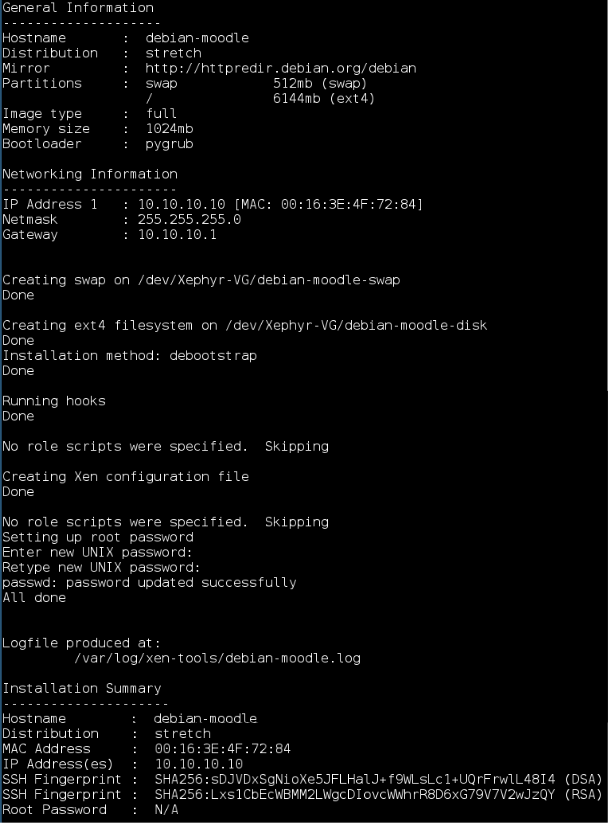
\includegraphics[width=0.75\textwidth]{Figures/crear-moodle.png}
    \end{center}
  	\caption{Crear maquina virtual para Moodle.}
    \label{vm-moodle}
\end{figure}

Se renombró el archivo de configuración de la maquina virtual generado en el paso anterior para temas de consistencia.

\begin{lstlisting}
	mv /etc/xen/debian-moodle.cfg\
    		/etc/xen/domU-debian-moodle.cfg
\end{lstlisting}

Un bug de Xen-Tools causa que no se instala correctamente un núcleo de Linux en la maquina virtual y por lo tanto es necesario entrar al mismo con un Chroot y instalar los paquetes faltantes (y hacer las adecuadas configuraciones  para permitir su arranque independiente de ayuda externa).

\begin{lstlisting}
	mount /dev/Xephyr-VG/debian-moodle-disk /mnt
	mount -o bind /proc /mnt/proc
	mount -o bind /sys /mnt/sys
	mount -o bind /dev /mnt/dev
	cp /etc/resolv.conf /mnt/etc/resolv.conf
	chroot /mnt /bin/bash
	apt install linux-image-amd64
	vim.tiny /boot/grub/menu.lst
	# Revisar que los archivos referenciados existen
	#		de verdad por ejemplo:
	# Replace initrd.img- con initrd.img
    # guarda y sale
	exit
	umount /mnt/proc            
	umount /mnt/sys 
	umount /mnt/dev 
	umount /mnt	
\end{lstlisting}

Para levantar la maquina virtual:

\begin{lstlisting}
	xl create /etc/xen/domU-debian-moodle.cfg -c
\end{lstlisting}

Se debe seleccionar la tercera opción (Default Kernel).

Se puede dar una revisión a la configuración de red para asegurarse de que esta correcto:

\begin{lstlisting}
	vim.tiny /etc/network/interfaces
\end{lstlisting}

Debe contener:

\begin{lstlisting}
auto eth0
iface eth0 inet static
 address 10.10.10.10
 gateway 10.10.10.1
 netmask 255.255.255.0
\end{lstlisting}

En el presente caso, Xen-Tools logró configurar esta parte de forma correcta.

A continuación se procede con la instalación de Moodle:

\begin{lstlisting}
# actualiza el sistema
apt update
apt upgrade

# instala dependencias
apt install apache2 php7.0 mysql-server php7.0-mysql
apt install libapache2-mod-php7.0 php7.0-gd php7.0-curl
apt install php-xml php-zip php-mbstring php-soap
apt install php7.0-xmlrpc php7.0-intl
vim.tiny /etc/php/7.0/apache2/php.ini

# agrega:
extension=mysql.so 
extension=gd.so

# edita:

memory_limit = 40M
# dejado con el valor por defecto de 128M

post_max_size = 80M
upload_max_filesize = 80M

# guarda y sale

# reinicia apache para coger los cambios
systemctl restart apache2

\end{lstlisting}

A continuación se configura la base de datos:

\begin{lstlisting}

# clave de root es root
mysqladmin -u root password "root"

# iniciar session como root
mysql -u root -p

# crear base de datos y hacer que ocupa UTF-8
mysql> CREATE DATABASE moodle;
mysql> ALTER DATABASE moodle charset=utf8;
mysql> exit;

## No se implemento ##
# Moodle queja de UTF8

# Se podria arreglar
# (antes de instalar Moodle)
# con:

mysql -u root -p

mysql> ALTER DATABASE moodle charset=utf8mb4;
mysql> exit;
######################

systemctl restart mysql

\end{lstlisting}

Se realiza la instalación de la ultima versión de Moodle (3.3 con sus respectivos patches de fallas desde que el mismo salio):

\begin{lstlisting}

# descargar
wget https://download.moodle.org/download.php/direct/stable33/moodle-latest-33.tgz

# descomprimir
tar -zxvf moodle-latest-33.tgz

# meter en la ubicacion para apache
mv moodle /var/www

# ir a ubicacion para apache
cd /var/www

# crear ubicacion para datos
mkdir moodledata

# arreglar permisos
chown -R www-data:www-data moodle
chown -R www-data:www-data moodledata
chmod -R 755 moodle
chmod -R 755 moodledata

# modificar configuracion de apache
vim.tiny /etc/apache2/sites-available/000-default.conf

# editar
DocumentRoot "/var/www/moodle"

# guardar y salir

# reiniciar apache para aplicar los cambios
systemctl restart apache2

\end{lstlisting}

Arreglar la base de datos para que acepte conexiones desde Moodle:

\begin{lstlisting}

mysql -u root -p

GRANT ALL PRIVILEGES on *.* to
	'root'@'localhost' IDENTIFIED BY 'root';
GRANT ALL PRIVILEGES on *.* to
	'root'@'localhost' IDENTIFIED BY 'root';
FLUSH PRIVILEGES;
exit;

\end{lstlisting}

Para seguir con la instalación se abre un navegador con la dirección \url{http://10.10.10.10/} para seguir las instrucciones que se le lleve por toda la configuración inicial del Moodle.

Al final se agregue un trabajo de cron para ayudar con los tareas periódicas que Moodle requiere para su mantenimiento continuo:

\begin{lstlisting}

crontab -u www-data -e
# add line:
*/10 * * * * /usr/bin/php
		/var/www/moodle/admin/cli/cron.php
        		>/dev/null

\end{lstlisting}

Estos pasos fueron adaptados de la guía oficial del proyecto de Moodle para instalación en Debian \citep{MOODLE-Install-Debian}.

Ahora que todo esta funcionando se recomienda editar /boot/grub/menu.lst para comentar las entradas del pyGrub que son defectuosas (los primeros dos) para que se puede levantar la maquina virtual sin intervención humana.

\subsubsection{Contenedor de Docker}
% TODO
% docker pull bitnami/mariadb
% docker pull bitnami/moodle

\index{Persistir Código} \index{Controlar Versiones de Código}
\subsection{Servidor de Git (GitLab CE)}
Originalmente fue planteada trabajar con GitLab Community Edition como una máquina virtual de Xen, pero con el tiempo, se ha visto una necesidad de consumir todos los servicios possibles de una forma mas liviana y por lo tanto aunque se incluye por este medio la instalación del mismo en una máquina virtual de Xen, al final se optó por un levantamiento del mismo en Docker.

\subsubsection{Máquina Virtual de Xen}
Para crear el servidor de Git con GitLab Community Edition, se va a empezar con las mismas piezas del servidor del LMS/Moodle, es decir una maquina virtual de Debian 9. El mismo se crea como una maquina virtual de Debian Stretch (9) con 1 GiB de RAM, 1 CPU virtual, 6 GiB de disco, 512 MiB de intercambio y una dirección IP fija de 10.10.10.11.
\begin{lstlisting}
	xen-create-image --hostname=debian-gitlab\
    		--ip=10.10.10.11 --netmask=255.255.255.0\
        	--gateway=10.10.10.1 --memory=1024mb\
        	--vcpus=1 --lvm=Xephyr-VG --pygrub\
        	--dist=stretch --force --size=6144mb\
        	--swap=512mb
\end{lstlisting}

Se renombró el archivo de configuración de la maquina virtual generado en el paso anterior para temas de consistencia.

\begin{lstlisting}
	mv /etc/xen/debian-gitlab.cfg\
    		/etc/xen/domU-debian-gitlab.cfg
\end{lstlisting}

Un bug de Xen-Tools causa que no se instala correctamente un núcleo de Linux en la maquina virtual y por lo tanto es necesario entrar al mismo con un Chroot y instalar los paquetes faltantes (y hacer las adecuadas configuraciones  para permitir su arranque independiente de ayuda externa).

\begin{lstlisting}
	mount /dev/Xephyr-VG/debian-gitlab-disk /mnt
	mount -o bind /proc /mnt/proc
	mount -o bind /sys /mnt/sys
	mount -o bind /dev /mnt/dev
	cp /etc/resolv.conf /mnt/etc/resolv.conf
	chroot /mnt /bin/bash
	apt install linux-image-amd64
	vim.tiny /boot/grub/menu.lst
	# Revisar que los archivos referenciados existen
	#		de verdad por ejemplo:
	# Replace initrd.img- con initrd.img
    # guarda y sale
	exit
	umount /mnt/proc            
	umount /mnt/sys 
	umount /mnt/dev 
	umount /mnt	
\end{lstlisting}

Para levantar la maquina virtual:

\begin{lstlisting}
	xl create /etc/xen/domU-debian-gitlab.cfg -c
\end{lstlisting}

Se debe seleccionar la tercera opción (Default Kernel).

Se puede dar una revisión a la configuración de red para asegurarse de que esta correcto:

\begin{lstlisting}
	vim.tiny /etc/network/interfaces
\end{lstlisting}

Debe contener:

\begin{lstlisting}
auto eth0
iface eth0 inet static
 address 10.10.10.11
 gateway 10.10.10.1
 netmask 255.255.255.0
\end{lstlisting}

En el presente caso, Xen-Tools logró configurar esta parte de forma correcta.

A continuación se procede con la instalación de Gitlab:

\begin{lstlisting}
# actualiza el sistema
apt update
apt upgrade

# A partir del Debian 9, Gitlab CE esta ofrecido
#    en los repositorios oficiales:
apt install gitlab

# Arreglar problema con API
vim.tiny /usr/share/gitlab-shell/config.yml
# cambiar gitlab_url a "http://10.10.10.11/"

/usr/share/gitlab-shell/bin/check
\end{lstlisting}

Visitar \url{http://10.10.10.11/} y configurar la contraseña del usuario root. Con el usuario root configurado se procede a crear un usuario especial para la aplicación con el nombre de usuario 'GitEdu'. Este usuario lo damos permisos de administración y también se genera un token en esta dirección: \url{http://10.10.10.11/profile/personal_access_tokens}. El token se debe guardar para su uso después (GitLab nunca le vuelve a mostrar).

Ahora que todo esta funcionando se recomienda editar /boot/grub/menu.lst para comentar las entradas del pyGrub que son defectuosas (los primeros dos) para que se puede levantar la maquina virtual sin intervención humana.

\subsubsection{Contenedor de Docker}
% TODO
% docker pull gitlab/gitlab-ce

\index{Ejecutar Código}
\subsection{Servidor de Virtualización}
Para la ejecución de código se considera necesario la virtualización. La ejecución puramente nativa de código daría mayor superficie de ataque al servidor físico además de no permitir mayor flexibilidad necesaria para sostener una gran variedad de usuarios y necesidades.

\subsubsection{Comparación de Hipervisores}
Para la selección de una tecnología de virtualización, se ha considerado conveniente realizar el siguiente cuadro comparativo en base a una valoración de características de cada ecosistema de hipervisor para generar una calificación ponderada de las mismas y poder llegar objetivamente al mejor hipervisor a ser implementado en el presente proyecto.

\begin{table}
	\centering
	\begin{tabular}{|l|r|}
    	\hline
		\textbf{Característica} & \textbf{Peso} \\
        \hline
        \textit{Rendimiento} & 10 \\
        \textit{Seguridad} & 10 \\
        \textit{Facilidad de Uso (CLI)} & 10 \\
        \textit{Facilidad de Uso (GUI)} & 5 \\
        \textit{Facilidad de Uso (WUI)} & 5 \\
        \textit{Facilidad de Instalación} & 5 \\
        \textit{Facilidad de Mantenimiento} & 5 \\
        \textit{Experiencia Personal del Autor} & 10 \\
        \hline
        \textbf{Total de Pesos} & 60 \\
        \hline
	\end{tabular}
    \caption{Pesos de las Características de Comparación para Hipervisores Considerados}
    \label{tab:hipervisor-compar-pesos}
\end{table}

El cuadro \ref{tab:hipervisor-compar-pesos} presenta las pesos que se asignaron a cada categoría de la comparación para poder realizar un promedio ponderado de las valoraciones con mayor peso en las categorías que se consideraban más importantes. Las características consideradas son:
\begin{description}
	\item[Rendimiento] Indica la máxima eficiencia que puede llegar a tener la virtualización con esta tecnología.
    \item[Seguridad] Indica el nivel de aislamiento y mitigación de riesgo que se considera los usuarios virtualizados frente la maquina host.
    \item[Facilidad de Uso (CLI)] La facilidad en utilizar el hipervisor desde linea de comandos (terminal).
    \item[Facilidad de Uso (GUI)] La facilidad en utilizar el hipervisor desde aplicación de escritorio gráfica.
    \item[Facilidad de Uso (WUI)] La facilidad en utilizar el hipervisor desde plataforma web.
    \item[Facilidad de Instalación] La facilidad para instalar el hipervisor y realizar la configuración inicial para que empieza a funcionar.
    \item[Facilidad de Mantenimiento] La facilidad para actualizar, utilizar y mantener el hipervisor.
    \item[Experiencia Personal del Autor] La opinión tiene el autor del hipervisor después de años de uso y experimentación en estas tecnologías.
\end{description}
Se ha considerado con mayor importancia el Rendimiento y la Seguridad como necesidades del presente proyecto. La Facilidad de Uso desde Línea de Comandos y la Experiencia Personal del Autor también se ha considerado importante para que se pueda implementar de forma mas concisa, rápida y precisa la tecnología de virtualización elegida. La Facilidad de Uso tanto Gráfica como Web en adición a la complejidad de Instalación y Mantenimiento se considera importantes pero menos relevantes debido a que son características de menor impacto para el desarrollo actual y al largo plazo donde tienen mayor impacto se puede implementar otra solución mas adecuada frente esos temas si es necesario. 

\begin{table}
	\centering
	\begin{tabular}{|p{1.85cm}|p{2.25cm}|p{1.8cm}|p{1.7cm}|p{1.7cm}|p{1.7cm}|}
    	\hline
		\textbf{Hipervisor} & \textbf{Rendimiento} & \textbf{Seguridad} & \textbf{Facilidad de Uso (CLI)} & \textbf{Facilidad de Uso (GUI)} & \textbf{Facilidad de Uso (WUI)} \\
        \hline
        \textit{Xen} & 4 & 5 & 4 & 3 & 2 \\
        \hline
        \textit{KVM} & 3 & 5 & 4 & 3 & 3 \\
        \hline
        \textit{Docker} & 5 & 3 & 5 & 3 & 4 \\
        \hline
	\end{tabular}
    \caption{Características de Comparación I: Hipervisores Considerados}
    \label{tab:hipervisor-compar-i}
\end{table}

\begin{table}
	\centering
	\begin{tabular}{|p{1.85cm}|p{2.2cm}|p{3.0cm}|p{1.9cm}|}
    	\hline
		\textbf{Hipervisor} & \textbf{Facilidad de Instalación} & \textbf{Facilidad de Mantenimiento} & \textbf{Experiencia Personal del Autor} \\
        \hline
        \textit{Xen} & 3 & 2 & 4 \\
        \hline
        \textit{KVM} & 4 & 2 & 2 \\
        \hline
        \textit{Docker} & 5 & 4 & 4 \\
        \hline
	\end{tabular}
    \caption{Características de Comparación II: Hipervisores Considerados}
    \label{tab:hipervisor-compar-ii}
\end{table}

% TODO: Correccion de la Maria del Carmen "caracteristicas consideradas"?
En los cuadros \ref{tab:hipervisor-compar-i} y \ref{tab:hipervisor-compar-ii} se presenta las características consideras y un puntaje relativo (sobre 5) dada a cada una de las mismas según las investigaciones, experiencias y opiniones del autor. A continuación se explica el porque de las valoraciones:
\begin{description}
	\item[Xen] como un hipervisor de tipo uno se cuenta con un rendimiento muy alto, especialmente cuando se toma en cuenta la paravirtualización que también se suporta con sistemas operativos modificados, casi a un nivel nativo. Este hipervisor logra virtualizar todas las capas de un sistema operativo, desde su núcleo hasta el espacio de los usuarios, pero al mismo tiempo dispone de un modelo de seguridad muy buena. Falla en las herramientas de administración de los cuales hay muy pocas que están actualizadas. La mejor herramienta de administración es en la Línea de Comandos. Sus cambios frecuentes y documentación desactualizada son un problema para la instalación y mantenimiento. La experiencia del autor con esta tecnología ha sido muy positiva.
    \item[KVM] como un hipervisor de tipo uno y medio es más alto nivel que Xen y no dispone del mismo nivel de rendimiento que ofrece ni la paravirtualización. Aunque es más alto nivel, se ha tomado pasos adicionales para que alcanza un nivel de seguridad equivalente a la de Xen. Para su administración cuenta con herramientas muy similares a los de Xen, pero su alto nivel de integración con el API de Libvirt hace que puente con mejores interfaces para su manejo web. Posiblemente por desconocimiento de las posibilidades para mejorar el rendimiento que se puede aplicar, el autor no ha tenido una experiencia muy positiva con la aplicación de esta tecnología de virtualización.
    \item[Docker] como un hipervisor de ''tipo tres'' es de muy alto nivel y dispone de una seguridad mucho menor al tener menor aislamiento entre el sistema que provee la virtualización y la virtualizada. Docker tiene mejor rendimiento ya que se virtualiza solo los niveles más altos de un sistema operativo y las aplicaciones que se encuentran por encima. Su técnica de containerización como un tipo de virtualización que puede dar mejor rendimiento que la paravirtualización. Se considera muy buena las interfaces para utilizar Docker, tanto a nivel de terminal como a nivel web. Puede que sea el caso por el hecho de que Docker es una tecnología que aún es bastante nueva y que esta en auge. Esto promueve una gran cantidad de personas a estar contribuyendo sus mejoras. La instalación y mantenimiento de Docker es muy sencillo en cualquier plataforma. Debido a su sencillez, alto rendimiento, funcionalidad y utilidad, el autor ha tenido una buena experiencia con el uso de esta tecnología de virtualización. 
\end{description}

Para calcular los pesos promediados de forma ponderada se aplica la siguiente formula que se encuentra en la figura \ref{fig:hipervisor-calif-equ}. Las calificaciones promedias se reflejan en el cuadro \ref{tab:hipervisor-compar-promed}. Como se puede observar del mismo cuadro, frente los criterios previamente establecidos, Docker se puede considerar la mejor tecnología de virtualización en el proyecto actual con un puntaje de $4.167$, con medio punto mas que su competencia mas cercana Xen, $3.667$ y $\frac{5}{6}$ de un punto mas que KVM, $3.333$, que esta en último lugar.

\begin{figure}
	\[
		Promedio = \sum_{c = [Categorías]} CalificaciónCatagoria_c * \left ( \frac{PesoCatagoria_c}{TotalPesos} \right )
	\]
	\caption{Ecuación para Calcular los Promedios Ponderados en base a Pesos para los Hipervisores Comparados}
    \label{fig:hipervisor-calif-equ}
\end{figure}

\begin{table}
	\centering
	\begin{tabular}{|l|r|}
    	\hline
		\textbf{Hipervisor} & \textbf{Calificación Promedio Ponderado} \\
        \hline
        \textit{Xen} & 3.667 \\
        \hline
        \textit{KVM} & 3.333 \\
        \hline
        \textit{Docker} & 4.167 \\
        \hline
	\end{tabular}
    \caption{Calificaciones Promediados Ponderadas para la Comparación de los Hipervisores}
    \label{tab:hipervisor-compar-promed}
\end{table}

\index{Hipervisor} \index{Virtualización} \index{Contenedor}
\subsubsection{Servidor de Virtualización Virtualizado}
% TODO
\paragraph{Instalación de Kubernetes}
% TODO
% # Kubernetes (Kubectl Client)
% curl -LO https://storage.googleapis.com/kubernetes-release/release/$(curl -s https://storage.googleapis.com/kubernetes-release/release/stable.txt)/bin/linux/amd64/kubectl
% chmod +x kubectl
% echo $PATH
% # move into $PATH
% mv kubectl ~/bin/
% # verify installation
% kubectl --help
% # or:
% kubectl version
% # will give server error, we only are a client thus far
\paragraph{MiniKube}
% TODO
% # Minikube
% curl -Lo minikube https://storage.googleapis.com/minikube/releases/v0.23.0/minikube-linux-amd64
% chmod +x minikube
% # move into $PATH
% mv minikube ~/bin/
% # verify installation:
% minikube --help
% # or
% minikube version
%
% # Start Minikube Cluster
% minikube start
%
% # Shutdown Minikube Cluster
% minikube stop

\paragraph{Máquina Virtual de Xen}
% TODO
\subsubsection{Construción de Servidor Virtualizado para Cluster de Kubernetes}
% TODO
% xen-create-image --hostname=debian-k8s-master --ip=10.10.10.12 --netmask=255.255.255.0 --gateway=10.10.10.1 --memory=2048mb --vcpus=2 --lvm=Xephyr-VG --pygrub --dist=stretch --force --size=10240mb --swap=1024mb
% see Screenshot_2017-12-29_15-21-49.png
\paragraph{Instalación de Docker}
% TODO
% apt update
% apt upgrade
% apt install curl
% curl -fsSL get.docker.com -o get-docker.sh
% sh get-docker.sh
% see Screenshot_2017-12-29_15-31-49.png
\paragraph{Instalación de Cluster de Kubernetes}
% TODO
%https://kubernetes.io/docs/setup/independent/install-kubeadm/
%apt-get update && apt-get install -y apt-transport-https
%curl -s https://packages.cloud.google.com/apt/doc/apt-key.gpg | apt-key add -
%cat <<EOF >/etc/apt/sources.list.d/kubernetes.list
%deb http://apt.kubernetes.io/ kubernetes-xenial main
%EOF
%apt-get update
%apt-get install -y kubelet kubeadm kubectl

%# Init Master
%kubeadm init
\index{Contenedor} \index{Virtualización} \index{Hipervisor}

\subsection{Plantillas de Máquinas Virtuales (Docker)}
Para la ejecución de código en Docker, es necesario tener un contenedor de Docker que cumpla con las dependencias requeridas al momento de la ejecución. Los contenedores están basados en Debian y en Alpine Linux.

\subsubsection{Sistema Operativo: Debian GNU/Linux}
Se considera Debian como una buena base para los contenedores debido a que es bastante conocido, estable, seguro y tiene una plenitud de paquetes que se pueden instalar directamente desde sus repositorios oficiales.

\subsubsection{Sistema Operativo: Alpine GNU/Linux}
Alpine Linux es muy utilizado en el mundo de los contenedores (por ejemplo con Docker) y en la nube en general porque es un sistema operativo minimalista que lleva menor peso. Aquí tiene el mismo fin, aunque aveces es mas complicado de manejar y configurar, puede que valga la pena para entornos de producción que necesitan optimizar el uso de sus recursos.

\subsubsection{Tipo de Contenedor: Shell-Executor}
El tipo de contenedor ''Shell-Executor'' es para ejecutar comandos dentro de un contenedor con el shell ''sh'' y forma la base para los otros tipos de contenedores. Tanto en Debian como en Alpine no hay necesidad de instalar más paquetes ya que el imagen por defecto viene con todo lo necesario. Lo que si se tiene que definir para estos contenedores es un usuario menos privilegiado con el cual se ejecuta los comandos/código dentro del contenedor y una ubicación, un volumen desde el punto de vista de Docker, donde se puede enviar el código a ser ejecutado. La diferencia entre la implementación tanto en Debian y Alpine es la creación de un usuario con menos privilegios en adición a la imagen base que se toma. 

% TODO: Mandar como anexo:
% TODO: Solo resumir aqui

El Debian Shell-Executor se crea con los siguientes lineas en el Dockerfile: 
\begin{lstlisting}
FROM debian:stretch

ENV shell=/bin/sh
ENV user=user

# Greatly increases image size, optional:
#RUN apt-get update && apt-get install -y lsb-release

RUN mkdir -p /code && echo "USER=$user" && echo "SHELL=$shell"\
&& useradd -ms $shell $user && chown -v $user:$user /code
VOLUME ["/code"]

ENTRYPOINT ["/bin/sh"]
CMD ["/code/exec.sh"]
\end{lstlisting}
La primera linea, ''FROM ...'' define el imagen base, en este caso la versión actual de Debian Stretch (Debian 9.x). La tercera y cuarta linea, ''ENV ...'', definen variables de entorno que se puede cambiar previa a la construcción del imagen en adición a sus valores por defecto. La sexta y séptima linea, documenta y define un paso opcional donde se instala un paquete adicional, lsb-release, que provee información estandarizado de la distribución de Linux en ejecución. Este paso opcional agrega mucho peso al contenedor y por lo tanto no se lo ha dejado comentado. La novena y décima linea define comandos preliminares para preparar el contenedor como:
\begin{itemize}
	\item Crear una carpeta "/code" donde se puede copiar el código a ser ejecutado desde afuera del contenedor
	\item Visualización los variables de entorno para temas informativos y de debug
	\item La creación del usuario que vamos a utilizar dentro del contenedor
	\item Dar el usuario los permisos adecuados para que tiene acceso a la carpeta creada
\end{itemize}
La onceava linea define la carpeta creada como un volumen de Docker, el cual se monta externamente al crear y ejecutar el contenedor. La decimotercera linea define el argumento cero del contenedor al momento de iniciar la misma, en este caso el shell que se encuentra del contenedor. La decimocuarta linea define los argumentos con que se debe ejecutar el comando definido previamente, en este caso el script de entrada, cargado desde un sistema de ficheros externo al contenedor.

El Alpine Shell-Executor se crea con los siguientes lineas en el Dockerfile: 
\begin{lstlisting}
FROM alpine:3.6

ENV shell=/bin/sh
ENV user=user

RUN mkdir -p /code && echo "USER=$user" && echo "SHELL=$shell"\
&& echo "SHELL is not used in this Dockerfile" &&\
    adduser -D $user && chown -v $user:$user /code
VOLUME ["/code"]

ENTRYPOINT ["/bin/sh"]
CMD ["/code/exec.sh"]
\end{lstlisting}
La primera linea, ''FROM ...'' define el imagen base, en este caso la versión actual de Alpine Linux (Alpine 3.6). La tercera y cuarta linea, ''ENV ...'', definen variables de entorno que se puede cambiar previa a la construcción del imagen en adición a sus valores por defecto. La sexta, séptima y octava lineas define comandos preliminares para preparar el contenedor como:
\begin{itemize}
	\item Crear una carpeta "/code" donde se puede copiar el código a ser ejecutado desde afuera del contenedor
	\item Visualización los variables de entorno para temas informativos y de debug
	\item La creación del usuario que vamos a utilizar dentro del contenedor
	\item Dar el usuario los permisos adecuados para que tiene acceso a la carpeta creada
\end{itemize}
La novena linea define la carpeta creada como un volumen de Docker, el cual se monta externamente al crear y ejecutar el contenedor. La onceava linea define el argumento cero del contenedor al momento de iniciar la misma, en este caso el shell que se encuentra del contenedor. La duodécima linea define los argumentos con que se debe ejecutar el comando definido previamente, en este caso el script de entrada, cargado desde un sistema de ficheros externo al contenedor.

\subsubsection{Tipo de Contenedor: Python3-Executor}
El tipo de contenedor ''Python3-Executor'' es para ejecutar comandos de shell en adición a código de Python 3. Se extiende de los contenedores definidos para el ''Shell-Executor'' para proveer funcionalidad de ejecutar comandos en un shell. El punto de entrada de ejecución es el archivo ''main.py'' a nivel raiz del repositorio. Tanto Debian como Alpine requieren la instalación de Python 3, porque lastimosamente su versión de Python por defecto sigue siendo 2.7 que se debería considerar prácticamente obsoleta. Docker requiere que se vuelve a definir los volúmenes y para la adecuada ejecución del código, también se define la ubicación inicial de ejecución como el mismo volumen que se monta desde un sistema de ficheros externo al contenedor.

El Debian Python3-Executor se define de la siguiente manera a través de su Dockerfile:
\begin{lstlisting}
FROM \
registry.gitlab.com/nishedcob/gitedu/shell-executor:debian-stretch

RUN apt-get update && apt-get install -y python3 python3-dev \
python3-pip virtualenv

VOLUME ["/code"]
WORKDIR "/code"
\end{lstlisting}
La primera y segunda linea define herencia del contenedor Debian Shell-Executor que definimos previamente. La tercera y cuarta linea instala Python3, Pip3 y Virtualenv dentro del contenedor. La sexta linea vuelve a declarar el volumen de Docker porque al aparecer la versión actual de Docker a propósito no suporta herencia de esta linea en los Dockerfile. La séptima linea define la ubicación inicial utilizada cuando se inicia el contenedor.

El Alpine Python3-Executor se define a través del Dockerfile que esta a continuación:
\begin{lstlisting}
FROM \
registry.gitlab.com/nishedcob/gitedu/shell-executor:alpine-3.6

RUN apk update && apk add python3 python3-dev py-virtualenv

VOLUME ["/code"]
WORKDIR "/code"
\end{lstlisting}
La primera y segunda linea define herencia del contenedor Alpine Shell-Executor que definimos previamente. La tercera linea instala Python3, Pip3 y Virtualenv dentro del contenedor. La quinta linea vuelve a declarar el volumen de Docker porque al aparecer la versión actual de Docker a propósito no suporta herencia de esta linea en los Dockerfile. La sexta linea define la ubicación inicial utilizada cuando se inicia el contenedor.

\subsubsection{Tipo de Contenedor: PostgreSQL-Executor}
El tipo de contenedor ''PostgreSQL-Executor'' es para ejecutar comandos de shell en adición a SQL de PostgreSQL. Se extiende de los contenedores definidos para el ''Shell-Executor'' para proveer funcionalidad de ejecutar comandos en un shell. El archivo ''init.sql'' se ejecuta primero y por lo tanto puede ser utilizado para generar y llenar la base de datos. El archivo ''main.sql'' se ejecuta después y por lo tanto podría ser útil para ejecutar comandos SQL definidos por el usuario. Tanto Debian como Alpine requieren la instalación de PostgreSQL, tanto cliente como servidor. Docker requiere que se vuelve a definir los volúmenes y para la adecuada ejecución del código, también se define la ubicación inicial de ejecución como el mismo volumen que se monta desde un sistema de ficheros externo al contenedor.

El Debian PostgreSQL-Executor se define con el siguiente Dockerfile:
\begin{lstlisting}
FROM \
registry.gitlab.com/nishedcob/gitedu/shell-executor:debian-stretch

RUN apt-get update && apt-get install -y postgresql \
postgresql-client

RUN echo "Starting PostgreSQL Cluster..." ; \
    /usr/bin/pg_ctlcluster 9.6 main start && \
    echo "Started cluster!" || \
    echo "Failed to start cluster!"; \
    su - postgres -c "createuser user && \
    createdb -O user userdb"; \
    echo "Stopping PostgreSQL Cluster..." ; \
    /usr/bin/pg_ctlcluster 9.6 main stop && \
    echo "Stopped cluster!" || \
    echo "Failed to stop cluster!";

VOLUME ["/code"]
WORKDIR "/code"
\end{lstlisting}
La primera y segunda linea define herencia del contenedor Debian Shell-Executor que definimos previamente. La tercera y cuarta linea instala PostgreSQL dentro del contenedor. La sexta hasta décima linea levanta el motor de base de datos PostgreSQL con la finalidad de crear un usuario y base de datos por defecto sobre el cual se puede trabajar. Finalizando este proceso se desactiva el contenedor para reducir el tamaño del mismo y no introducir comportamiento desconocido. La duodécima linea vuelve a declarar el volumen de Docker porque al aparecer la versión actual de Docker a propósito no suporta herencia de esta linea en los Dockerfile. La decimotercera linea define la ubicación inicial utilizada cuando se inicia el contenedor.

El Alpine PostgreSQL-Executor se define con el siguiente Dockerfile:
\begin{lstlisting}
FROM \
registry.gitlab.com/nishedcob/gitedu/shell-executor:alpine-3.6

RUN apk update && apk add postgresql && su - postgres -c \
"export PGDATA=/var/lib/postgresql/data && initdb"

RUN echo "Starting PostgreSQL Cluster..." ; \
    mkdir -p /run/postgresql && chown -R postgres:postgres \
    /run/postgresql && chmod 755 /run/postgresql && \
    mkdir -p /var/run/postgresql && chown -R postgres:postgres \
    /var/run/postgresql && \
    chmod 2777 /var/run/postgresql && su - postgres -c \
    "export PGDATA=/var/lib/postgresql/data && postgres &" && \
        echo "Started cluster!" || echo "Failed to start cluster!"; \
    sleep 5s && netstat -tupln && \
    su - postgres -c "createuser user && createdb -O user userdb"; \
    echo "Stopping PostgreSQL Cluster..." ; killall postgres && \
        echo "Stopped cluster!" || echo "Failed to stop cluster!";

VOLUME ["/code"]
WORKDIR "/code"
\end{lstlisting}
La primera y segunda linea define herencia del contenedor Alpine Shell-Executor que definimos previamente. La tercera y cuarta linea instala PostgreSQL dentro del contenedor en adición a inicializar la base de datos. La sexta hasta decimoséptima linea levanta el motor de base de datos PostgreSQL con la finalidad de crear un usuario y base de datos por defecto sobre el cual se puede trabajar. Finalizando este proceso se desactiva el contenedor para reducir el tamaño del mismo y no introducir comportamiento desconocido. La decimonovena linea vuelve a declarar el volumen de Docker porque al aparecer la versión actual de Docker a propósito no suporta herencia de esta linea en los Dockerfile. La vigésima linea define la ubicación inicial utilizada cuando se inicia el contenedor.

\section{GitEDU}

La gestión de dependencias del sistema GitEdu se maneja con un entorno virtual y el gestor de paquetes de python pip. El siguiente es un script de bash diseñado a detectar si es que existe el entorno virtual (lo crea en caso de que no existe) y después instala los requerimientos faltantes como son especificados en un archivo aparte ''requirements.txt'' que da librerías y sus versiones.

\begin{lstlisting}

# run with `source activate.sh` 
if [ ! -d env ]; then
	virtualenv --python=python3 env
fi
source env/bin/activate
pip3 install -r requirements.txt

\end{lstlisting}

El script anterior se ejecuta desde el raiz del repositorio con el comando:

\begin{lstlisting}
source activate.sh
\end{lstlisting}

Con el entorno creado y activado se puede proceder a instalar cualquier dependencia necesaria que no ha sido instalado previamente:

\begin{lstlisting}
pip install <nombre_dependencia>
\end{lstlisting}

Para el presente proyecto se instalaron las siguientes dependencias:
\begin{itemize}
	\item Django (1.10.6) como framework para el desarrollo del backend.
    \item Psycopg2 (2.7.1) como librería para conectarse a bases de datos PostgreSQL.
    \item Python-GitLab (0.20) como librería para consumir el API de GitLab.
    \item ipython (6.1.0) como interprete interactivo de Python para hacer pruebas en el curso del desarrollo.
\end{itemize}

Con las dependencias instaladas o con cada cambio que se realiza de dependencias se ejecuta el siguiente comando para actualizar la lista de los mismos:

\begin{lstlisting}
pip freeze > requirements.txt
\end{lstlisting}

Se inicia el proyecto de Django con el comando:

\begin{lstlisting}
django-admin startproject GitEdu
\end{lstlisting}

También antes de iniciar el desarrollo debe estar configurado el base de datos para ocupar el mismo. Primero es necesario crear y configurar un usuario y base de datos para ser ocupado:
\begin{lstlisting}
postgresql-setup initdb
systemctl enable postgresql
systemctl start postgresql
systemctl status postgresql
vim /etc/postgresql/9.6/main/pg_hba.conf
# agregar una linea antes de las lineas similares y
# que diga (sin el numeral adelante):
#local   all      postgres             peer
systemctl restart postgresql
systemctl status postgresql
su - postgres
psql
\end{lstlisting}
\begin{lstlisting}
	postgres=# CREATE USER giteduser WITH PASSWORD 'g1T3d_$3r';
	postgres=# CREATE DATABASE gitedudb WITH OWNER giteduser;
	postgres=# \q
psql gitedudb -U postgres
	gitedudb=# CREATE SCHEMA giteduapp AUTHORIZATION giteduser;
	gitedudb=# ALTER USER giteduser SET search_path TO giteduapp;
	gitedudb=# \q
psql gitedudb -U giteduser
	gitedudb=> SELECT current_schema();
		Debe decir: giteduapp
	gitedudb=> \q
\end{lstlisting}

Segundo, se abre el settings.py (dentro de la carpeta GitEDU/GitEDU) y se remplaza (para desarrollo, en producción debe llevar valores distintos) el atributo DATABASES con lo siguiente:
\lstset{language=Python}
\begin{lstlisting}
DATABASES = {
    'default': {
        'ENGINE': 'django.db.backends.postgresql_psycopg2',
        'NAME': 'gitedudb',
        'USER': 'giteduser',
        'PASSWORD': 'g1T3d_$3r',
        'HOST': '127.0.0.1',
        'PORT': '5432',
    }
}
\end{lstlisting}
\lstset{language=Bash}

Ahora se puede migrar las tablas iniciales de Django:
\begin{lstlisting}
cd GitEDU
python manage.py makemigrations
python manage.py migrate
\end{lstlisting}

También creamos un superusuario de Django para temas administrativos:
\begin{lstlisting}
python manage.py createsuperuser
\end{lstlisting}

También se puede crear el app inicial (para lógica del editor de código):
\begin{lstlisting}
python manage.py startapp ideApp
\end{lstlisting}

Y de paso se lo agrega a INSTALLED\_APPS una linea 'ideApp' en el settings.py para que sus tablas definidos a futuro en models.py también se migran con los demás migraciones.

Para resolver un problema de zonas de tiempo, se ha desactivado esta característica de Django con el siguiente linea en el settings.py:
\lstset{language=Python}
\begin{lstlisting}
USE_TZ = False
\end{lstlisting}
\lstset{language=Bash}

Para crear la base de datos de MongoDB:
\begin{lstlisting}
mongo
\end{lstlisting}
\lstset{language=sql}
\begin{lstlisting}
use gitEduDB
db.createUser(
    {
        user: "gitEduUser",
        pwd: "G1TedU$3r",
        roles: [ "readWrite", "dbAdmin" ]
    }
)
\end{lstlisting}
\lstset{language=Bash}

El mismo se define en el settings de la siguiente manera:
\lstset{language=Python}
\begin{lstlisting}
NOSQL_DATABASES = {
    'nosql': {
        'NAME': 'gitEduDB',
        'USER': "gitEduUser",
        'PASSWORD': 'G1TedU$3r',
        'HOST': '127.0.0.1',
        'PORT': '27017',
    }
}
\end{lstlisting}
\lstset{language=Bash}

\subsubsection{Compatibilidad con EduNube en el Mismo Repositorio}
Para reducir el numero de repositorios involucrados en este trabajo de titulación, se ha optado por llevar el desarrollo de EduNube dentro del mismo repositorio, con una separación de dependencias con otro entorno virtual y aislamiento de código en desarrollo con varias ramas de Git. Por lo tanto, se realizo una nueva rama de Git con el comando:
\begin{lstlisting}
git checkout -b gitedu
\end{lstlisting}

Y una refacturación del entorno virtual a ser ''env-ge'' en lugar de ''env'', en lugar de ''requirements.txt'', utilizar ''requirements.ge.txt'' y un nuevo script de activar el entorno, el cual se activa ahora con ''source activate-ge.sh'':
\begin{lstlisting}
#! /usr/bin/head -n 2 
# run with `source activate-ge.sh`
PROJECT=ge
ENV_DIR=env-$PROJECT
if [ ! -d $ENV_DIR ]; then
	virtualenv --python=python3 $ENV_DIR
fi
source $ENV_DIR/bin/activate
pip3 install -r requirements.$PROJECT.txt
\end{lstlisting}

Para desarrollar ambos sistemas en paralelo, y poder trabajar en ramas independientes con ambos sistemas levantados al mismo tiempo para probar y desarrollar características de integración, se clono de forma local el repositorio:
\begin{lstlisting}
git clone GitEDU GitEDU-copy
\end{lstlisting}

Para el desarrollo se ocupa el puerto 8000 de localhost para GitEDU y el puerto 8001 de localhost para EduNube:
\begin{lstlisting}
# Levantar GitEDU en el ambiente de desarrollo:
cd GitEDU-copy
source activate-ge.sh
git checkout gitedu
cd GitEDU
python manage.py runserver 8000

# Levantar EduNube en el ambiente de desarrollo:
cd GitEDU
source activate-en.sh
git checkout edunube
cd EduNube
python manage.py runserver 8001
\end{lstlisting}

\subsection{Autenticación Clásica}

Primero se crea una nueva aplicación para autenticación clásica:
\begin{lstlisting}
python manage.py startapp authApp
\end{lstlisting}

Y de paso se lo agrega a INSTALLED\_APPS una linea 'authApp' en el settings.py para que sus tablas definidos a futuro en models.py también se migran con los demás migraciones.

Para la implementación de autenticación clásica, se reutilizo el modulo con el mismo propósito del proyecto anterior GitEduERP. A esta se aumento la funcionalidad adicional de que desde el settings se puede activar o desactivar la funcionalidad de permitir a usuarios registrarse a través del atributo ENABLE\_REGISTRATION. 

Para el registro de usuarios, se considera que solo debe permitirse (en caso de que sea habilitado por la administración) el registro de estudiantes y docentes pero no de administradores, motivo por el cual se ha considerado duplicar los formularios de registro y ofrecer uno para estudiantes y otro para docentes. Los mismos se pueden habilitar y deshabilitar con los atributos ENABLE\_STUDENT\_REGISTRATION y ENABLE\_TEACHER\_REGISTRATION respectivamente.

\index{Autenticación LTI}
\subsection{Autenticación por LTI}

Primero es necesario que este activo y levantado el ambiente del LMS \index{LMS} como se documenta en la sección \ref{instalacion-moodle} de instalación de Moodle. Para el desarrollo de este trabajo de titulación se esta considerando una instalación en un servidor aparte (virtualizado en el mismo equipo) en la dirección IP 10.10.10.10.

% Instalar dependencias

Instalación de dependencias desde GitHub (no se encuentran en los repositorios oficiales de Pip/Pypi; además para superar problemas de dependencias en las librerías, se ha optado para ocupar forks personales del autor con las mejores necesarias para su funcionamiento):
\begin{lstlisting}
pip install git+https://github.com/nishedcob/django-app-lti
    @master#egg=django-app-lti
pip install git+https://github.com/nishedcob/
    django-auth-lti@master#egg=django-auth-lti
\end{lstlisting}

Como son dependencias no se encuentran en los repositorios oficiales, su manejo dentro del requirements.txt también tiene que ser especial ya que un `pip freeze` no los guardaran correctamente dentro del mismo. En lugar de eso hay que agregar dos lineas al requirements.txt para el manejo de estas dependencias:
\begin{lstlisting}
-e git+https://github.com/nishedcob/django-app-lti.git
    @38b32989e22b189345e421b183684f9b5453e99a
    #egg=django-app-lti
-e git+https://github.com/nishedcob/django-auth-lti.git
    @71c9da8d0aa07ebc3139bf3f113b5c521d61b1f1
    #egg=django-auth-lti
\end{lstlisting}

% Modificar settings

\lstset{language=Python}

Se pone a editar el settings.py (dentro de GitEDU/GitEDU) con las siguientes configuraciones:
\begin{itemize}
	\item a INSTALLED\_APPS agregamos las siguientes lineas:
   		\begin{lstlisting}
    'django_auth_lti',
    'django_app_lti',
    	\end{lstlisting}
    \item a MIDDLEWARE agregamos la siguiente linea:
   		\begin{lstlisting}
    'django_auth_lti.middleware.LTIAuthMiddleware',
    	\end{lstlisting}
    \item a AUTHENTICATION\_BACKENDS agregamos la siguiente linea:
   		\begin{lstlisting}
    'django_auth_lti.backends.LTIAuthBackend',
    	\end{lstlisting}
        Si es que no existe AUTHENTICATION\_BACKENDS lo creamos con los siguientes valores:
        \begin{lstlisting}
AUTHENTICATION_BACKENDS = (
    'django.contrib.auth.backends.ModelBackend',
    'django_auth_lti.backends.LTIAuthBackend',
)
        \end{lstlisting}
    \item también agregamos los siguientes atributos:
    	\begin{itemize}
    		\item LTI\_SETUP
            	\begin{lstlisting}
LTI_SETUP = {
    "TOOL_TITLE": "GitEDU",
    "TOOL_DESCRIPTION": "Sistema para Programar en Linea",
    "LAUNCH_URL": "lti:launch",
    "LAUNCH_REDIRECT_URL": "ideApp:decode",
    "INITIALIZE_MODELS": False,
    "EXTENSION_PARAMETERS": {
        "10.10.10.10": {
            "privacy_level": "public",
            "course_navigation": {
                "enabled": "true",
                "default": "disabled",
                "text": "GitEDU LMS Playground",
            }
        }
    }
}
            	\end{lstlisting}
            \item LTI\_OAUTH\_CREDENTIALS con texto aleatorio (fue ocupado OpenSSL, específicamente el comando \texttt{openssl rand -hex 10} para generar los valores de abajo\footnote{Un ambiente de producción debe ocupar valores distintos}).
            	\begin{lstlisting}
LTI_OAUTH_CREDENTIALS = {
    "GitEduLMS_Playground": "b2e0158c3cb4ddb0202d", 
         # (Para pruebas)
    "GitEduLMS_Playground_Assignments":
         "57b3a14734566c49bcaf",
         # (Para deberes/examenes/pruebas/talleres/etc)
    "GitEduLMS_Playground_Classes":
         "f7a0b6accc2631779e84",
         # (Para materias)
}
            	\end{lstlisting}
    	\end{itemize}
\end{itemize}

También se edita el urls.py (dentro de la misma dirección que el settings.py) con las siguientes lineas:
\begin{lstlisting}
from django.conf.urls import include
import django_app_lti.urls

# dentro de:
urlpatterns = [
    # agregar:
    url(r'^lti/', include(django_app_lti.urls, namespace="lti")),
]

\end{lstlisting}

\lstset{language=Bash}

Para arreglar un problema de una versión muy desactualizada de ims-lti-py, se agrego la siguiente linea al requirements.txt (para ocupar un fork del propio librería por el propio autor para resolver los problemas dados):
\begin{lstlisting}
-e git+https://github.com/nishedcob/ims_lti_py.git
    @a6576d7892ea4f69b76572788b118aaa4cdcf749
    #egg=ims_lti_py-develop
\end{lstlisting}

Para arreglar un problema de limpieza de datos en oauth2, se agrego la siguiente linea al requirements.txt (para ocupar un fork del propio librería por el propio autor para resolver los problemas dados):
\begin{lstlisting}
-e git+https://github.com/nishedcob/python-oauth2.git
    @176fc35aa35d626afcb6a23459482a4c96782c88
    #egg=oauth2
\end{lstlisting}

Después se migra la base de datos:
\begin{lstlisting}
python manage.py makemigrations
python manage.py migrate
\end{lstlisting}

\subsubsection{Validación}

Se levanta la aplicación (en \url{http://localhost:8000/} con:
\begin{lstlisting}
python manage.py runserver
\end{lstlisting}
La maquina virtual de Moodle también debe estar levantado para navegar a \url{http://10.10.10.10/}, iniciarse sesión como administrador, ir a la parte administrativa, a la pestaña de ''development'', seleccionar ''debugging'', y poner ''debug messages'' a nivel ''developer''. Ahora podemos volver a la parte de administración, volver a seleccionar la pestaña de ''development'' y crear un curso de prueba. Vamos a crear un curso pequeña (10 MB) con el nombre corto ''Prog\_I'' y nombre larga / descripción ''Introducción a la Programación''. Una vez que nos carga el curso, activamos modo de editar y agregamos una actividad externa.

Se da un nombre a la actividad, en este caso ''Prueba 1 Programación''. La mejor forma de poder reutilizar la herramienta externa en varias actividades es de crear una herramienta ''Preconfigurada''. Las opciones elegidas para la misma fueron los siguientes:
\begin{description}
	\item[Nombre] GitEdu
    \item[URL] \url{http://localhost:8000/lti/launch}
    \item[Descripción] Edit Code Online
    \item[Llave de Consumidor] GitEduLMS\_Playground
    \item[Secreto Compartido] b2e0158c3cb4ddb0202d
    \item[Parámetros Adicionales] lo dejamos en blanco
    \item[Contenedor de Lanzamiento] Nueva ventana
    \item[Compartir Nombre] Siempre
    \item[Compartir Correo Electrónico] Siempre
    \item[Aceptar Notas] Siempre
\end{description}
Con la herramienta preconfigurada realizada, se puede seleccionarlo así no mas para completar la integración. Donde se creó la actividad debe haber un enlace con el nombre del mismo, en este caso ''Prueba 1 Programación''. Al abrir el enlace se debe llevar a la aplicación con lo siguiente puntos interesantes:
\begin{enumerate}
	\item se encuentra autenticado con el mismo usuario de Moodle (incluyendo sus roles como ''administrador'', ''instructor'', ''estudiante'', etc\ldots{})
    \item hay contexto de:
    \begin{enumerate}
    	\item el curso de origen de Moodle
        \item la actividad de origen de Moodle (no es contexto completo, un problema que se tendrá que resolver en el curso del desarrollo)
        \item el llave de consumidor ocupado
    \end{enumerate}
\end{enumerate}

Si, dentro del mismo curso creamos una segunda actividad con todo lo mismo, pero solo cambiando el nombre a ''Prueba 2 Programación'', se encuentra que si logra distinguir entre actividades.

\subsection{Integración de Dos Schemas de Autenticación}
Los dos schemas de autenticación implementadas, sea la forma clásica con nombre de usuario y contraseña correspondiente o por LTI \index{LTI} donde una aplicación externa autentica un usuario autenticado previamente por el mismo, tienen un mismo fin de permitir que el sistema conozca quien esta accediendo el sistema con un fin de dar el comportamiento adecuado y en base a ello proveer seguridad y funcionalidad adecuado a todos los usuarios según su rol.

Para el mismo se propone tres tablas (EquivalentUser, AuthenticationType, UserAuthentication) en la base de datos expresados como modelos de Django, los cual se encargara de generar las tablas adecuadas en la base de datos a traves de su ORM interna.

La tabla EquivalentUser relaciona usuarios autenticados de forma clásica con usuarios autenticados por LTI \index{LTI} (porque por cada método de autenticación se cree un nuevo usuario para su propio uso interno) con un fin de permitir relacionar distintos usuarios dentro del sistema quienes representan el mismo individuo natural. El idea es por ejemplo, si un docente se autentica por LTI \index{LTI} y también por usuario y contraseña, para el sistema esta ocupando dos usuarios diferentes pero para el docente esta accediendo el mismo sistema y por lo tanto el comportamiento del sistema, sin tomar en cuenta como se autentica, debe ser igual y debe tener acceso a los mismos contenidos. La tabla AuthenticationType es un catalogo de formas de autenticación que suporta el sistema y por su naturaleza de catalogo se llena con las migraciones. Y finalmente la tabla UserAuthentication documenta el tipo de autenticación asociado con un usuario para dar el contexto al sistema que necesita para manejar distintos datos de los diferentes tipos de usuarios.

Con una migración se puede llenar de forma automática el catalogo de AuthenticacionType:
\lstset{language=Python}
\begin{lstlisting}
def fill_auth_types(apps, schema_editor):
    auth_type = models.AuthenticationType
    classic = auth_type(name="Clasica")
    classic.save()
    lti = auth_type(name="LTI")
    lti.save()


class Migration(migrations.Migration):

    dependencies = [
        ('authApp',
           '0002_authenticationtype_userauthentication'),
    ]

    operations = [
        migrations.RunPython(fill_auth_types),
    ]
\end{lstlisting}
\lstset{language=Bash}

\subsection{Accesibilidad a Datos de Autenticación de LTI}
Primero al settings se agrega dos atributos que indiquen cual llave se considera el sistema para compartir materias y otro para compartir deberes/exámenes/pruebas/talleres/etc\ldots{}:
\lstset{language=Python}
\begin{lstlisting}
LTI_ASSIGNMENTS_KEY = 'GitEduLMS_Playground_Assignments'
LTI_CLASSES_KEY = 'GitEduLMS_Playground_Classes'
\end{lstlisting}
\lstset{language=Bash}

Para controlar las partes de la configuración que se presenta a los usuarios finales, agregamos un nuevo campo de configuración al settings:
\lstset{language=Python}
\begin{lstlisting}
LTI_CONFIG_EXPOSE = {
    "LTI_KEYS": True,
    "LTI_ASSIGNMENT_KEY": True,
    "LTI_CLASS_KEY": True,
    "LTI_OTHER_KEYS": False,
    "LTI_SETUP": False,
}
\end{lstlisting}
\lstset{language=Bash}

Para que los profesores (como usuario final de GitEdu) también tengan acceso a estos credenciales para poderlos ocupar, se cree una vista en la ubicación '/auth/lti/credentials' que devuelve un JSON con los datos de LTI:
\lstset{language=Python}
\begin{lstlisting}
class LTICredentialsView(View):

    def get(self, request):
        if not request.user.is_authenticated:
            raise PermissionError("No tiene acceso a esta\
                vista hasta que se autentica...")

        lti_expose = settings.LTI_CONFIG_EXPOSE

        lti_cred_json = {}

        if lti_expose['LTI_KEYS']:
            if lti_expose['LTI_ASSIGNMENT_KEY']:
                lti_cred_json['LTI_ASSIGNMENT_KEY'] = {
                    settings.LTI_ASSIGNMENTS_KEY: 
                        settings.LTI_OAUTH_CREDENTIALS
                            [settings.LTI_ASSIGNMENTS_KEY]
                }
            if lti_expose['LTI_CLASS_KEY']:
                lti_cred_json['LTI_CLASS_KEY'] = {
                    settings.LTI_CLASSES_KEY:
                        settings.LTI_OAUTH_CREDENTIALS
                            [settings.LTI_CLASSES_KEY]
                }
            if lti_expose['LTI_OTHER_KEYS']:
                lti_cred_json['LTI_OTHER_KEYS'] =
                    settings.LTI_OAUTH_CREDENTIALS

        if lti_expose['LTI_SETUP']:
            lti_cred_json['LTI_SETUP'] =
                settings.LTI_SETUP

        return JsonResponse(lti_cred_json)
\end{lstlisting}
\lstset{language=Bash}

\index{Calificar Código}
\subsection{Establecer un Modelo de Base de Datos}
Para empezar con el desarrollo de la parte fuerte del sistema GitEDU, es importante considerar su modelo de base de datos preliminar. La parte mas importante de ello es las tablas o entidades y las relaciones entre las mismas. Para el mismo se ha considerado 3 grupos de funcionalidad importantes:
\begin{enumerate}
	\item El aspecto social y con ello los varios roles que pueden jugar usuarios dentro del sistema. Esto se representa con el app 'socialApp'.
    \item El aspecto academico y con ello como se llevan las materias académicas dentro del sistema. Esto se representa con el app 'academicApp'.
    \item El aspecto de notas y con ello la forma en que se llevan las notas que estudiantes sacan en las materias. Este aspecto lleva mucha en común con el aspecto anterior de la parte academico y la linea que les divide es un poco subjetiva por el mismo hecho de que no se ha optado por la creación de tablas adicionales para separar los dos, pero donde ha sido posible, se ha realizado la división. Este aspecto se representa con el app 'gradesApp'. 
\end{enumerate}

\begin{lstlisting}
python manage.py startapp socialApp
python manage.py startapp academicApp
python manage.py startapp gradesApp
\end{lstlisting}

Cada uno de los anteriores ha sido agregado al INSTALLED\_APPS del settings para que Django reconozca la necesidad de tomar en cuenta los modelos de cada uno.

Los modelos iniciales del socialApp solo definen distintos roles sociales dentro del sistema y ocupan de cuatro tablas:
\begin{enumerate}
	\item Person
	\item Student
	\item Teacher
	\item Administrator
\end{enumerate}
Se esta tomando en cuenta que la tabla de usuarios de Django ya lleva por defecto muchos detalles de los usuarios como sus nombres y apellidos y por lo tanto no hay necesidad de replicar estos datos. Esta hierarquia de clases mas bien viene a dar la infraestructura necesaria para especializar cada uno de estos en caso de que sea necesario.

El modelo inicial de academicApp permite a docentes y administradores definir materias ofrecidos (con paralelos y metadatos como categoría del componente), involucrados en los mismos, sean los mismos docentes o sus estudiantes, en adición a proveer la infraestructura de datos necesario para que un docente puede definir su libreta de calificaciones para una materia en base a un sistema relativo o un sistema de promedios ponderados (que el sistema puede calcular en base al sistema relativo). Esto involucra nueve tablas en la base de datos:
\begin{enumerate}
  \item ClassSubject
  \item Course
  \item Section
  \item Classroom
  \item ClassroomTeacher
  \item ClassroomStudent
  \item AcademicCategory
  \item AcademicSubCategory
  \item AcademicAssignment
\end{enumerate}
ClassSubject define el tipo de materia que es, por ejemplo ''Programación'' o ''Base de Datos''. Course define una materia ofrecida, por ejemplo ''Introducción a la Programación''. Section define paralelos ofrecidos de forma general, por ejemplo ''A'', ''B'', ''C'', etc\ldots{} Classroom une las dos tablas anteriores de materia de oferta con paralelo para definir aulas de una materia. ClassroomTeacher define el docente asignado a una aula y el peso que tiene el docente en la nota final de los estudiantes de esta aula. Esto es con un fin de permitir varios docentes con varios pesos dentro de la misma aula emitiendo calificaciones distintas para estudiantes previo a un promedio ponderado del estudiante. ClassroomStudent relaciona estudiantes y aulas. AcademicCategory provee docentes con la oportunidad de disponer de una herramienta para organizar las calificaciones de sus estudiantes en categorías con distintos pesos, por ejemplo ''Exámenes'', ''Deberes'', ''Talleres'', etc\ldots{} AcademicSubCategory viene de la misma linea para permitir subdivisiones de las categorías. AcademicAssignment es la abstracción que se da a los itemes calificadas dentro de una subcatagoría.

El modelo inicial de gradesApp permite persistir notas para cada estudiante bajo el modelo de tres niveles definido previamente de categorías, subcatagorías y itemes de subcatagorías con tres tablas:
\begin{enumerate}
  \item StudentCategoryGrade
  \item StudentSubCategoryGrade
  \item StudentAssignmentGrade
\end{enumerate}

\index{Editar Código}
\subsection{Editor de Código en Linea}
Una de las funcionalidades principales del sistema GitEDU es la capacidad de editar código en linea, la lógica del mismo se realiza en la app 'ideApp'.

Con relación al editor de código en linea, inicialmente se empezó con el trabajo realizado anteriormente en el proyecto GitEduERP y en base al mismo se fue expandiendo las características necesarias en el nuevo sistema. Durante el proceso del desarrollo, se observó una necesidad de desarrollar la mayoría de los componentes desde cero y con el mismo se pudo dar mejoras a la propuesta anterior. A diferencia de GitEduERP, GitEDU espera ofrecer:
\begin{itemize}
  \item Un modelo de permisos más robusto y flexible basado en grupos y usuarios.
  \item Un sistema de persistencia de código el cual ofrece la siguientes características:
    \begin{itemize}
      \item Ser extensible con una programación orientada a objetos.
      \item Manejar versiones de código con un sistema de control de versiones interna llevada por archivos completos
      \item Manejo de jerarquías de sistemas de persistencia para llevar varias sistemas de persistencia en paralelo
    \end{itemize}
   \item Integración con sistemas externas que permiten la ejecución de código.
\end{itemize}

\subsubsection{Modelo de Base de Dato para Editor de Código}
Para el editor de código en linea, es necesaria extender la funcionalidad del modelo de base de datos introducido previamente. Primero se agrega dos entidades a socialApp que representan grupos de personas (usuarios) y membresía dentro de estos mismos grupos con dos tablas:
\begin{enumerate}
\item Group
\item GroupMembership
\end{enumerate}

Dentro de ideApp se crea 4 entidades para representar repositorios (una colección de archivos asociados con un proyecto), el mismo tiene capacidad de un usuario y opcionalmente grupo dueño quien esta encargado de la administración del mismo, archivo mismo que entre sus metadatos esta un lenguaje asociado para ayudar con el manejo del mismo a nivel de editor y a nivel de otros tipo de gestión (como ejecución y compilación), y finalmente membresía de personas y grupos en repositorios con una finalidad de llevar mas adelante un sistema de permisos para restringir acceso y/o otras acciones sobre código por usuarios no autorizados. Estos entidades como tablas en la base de datos son:
\begin{enumerate}
\item Repository
\item File
\item RepositoryPersonMembership
\item RepositoryGroupMembership
\end{enumerate}

% <TODO>
%\subsubsection{Sincronizar y guardar en tiempo real}
% </TODO>

\index{Persistir Código}
\subsection{Persistencia de Código}
Para la Persistencia de Código se considera dos backends de persistencia para código con una posibilidad de introducir mas a futuro:
\begin{itemize}
	\item MongoDB como base de datos NoSQL para acceso rápido y recuperación de código persistido de una manera similar a GitEduERP.
    \item GitLab CE, como servidor de Git, manejado con una combinación de la API del mismo y comandos de Git para el manejo de cambios en repositorios.
\end{itemize}

Para el mismo es necesario manejar un API interna estandarizada. La solución propuesta utiliza programación orientado a objetos y un modelo estándar de namespace (como usuario o grupo) que contiene repositorios (que representan proyectos o conjuntos lógicos de archivos) y a su vez contienen dichos archivos. La clase base para estandarización se llama CodePersistenceBackend y se encuentra en generics.py del paquete ideApp.CodePersistenceBackends. Para el manejo de datos dentro del API interna, se estandariza los objetos de datos con las siguientes clases genéricas, las cuales pueden ser sobrescritas en cualquier backend con una finalidad de agregar o cambiar funcionalidad existente. Los mismos también se encuentran en el mismo archivo de generics.py. Estos archivos se puede encontrar en el Apéndice \ref{AnexoF}.

En el settings, hay una necesidad de definir los backends de código y su prioridad:
\lstset{language=Python}
\begin{lstlisting}[breaklines]
CODE_PERSISTENCE_BACKENDS = {
    'mongodb': {
        'use': True,
        'backend': 'ideApp.CodePersistenceBackends.MongoDB.backend.MongoDBCodePersistenceBackend',
        'connection_profiles': NOSQL_DATABASES,
        'connection_profile': 'nosql',
    },
    'gitlab': {
        'use': False,
        'backend': 'ideApp.CodePersistenceBackends.GitLab.backend.GitLabCodePersistenceBackend',
        'connection_profiles': GITLAB_SERVERS,
        'connection_profile': GITLAB_DEFAULT_SERVER,
    }
}

CODE_PERSISTENCE_BACKEND_READ_PREFERENCE = ['mongodb']
CODE_PERSISTENCE_BACKEND_WRITE_OUT = ['mongodb']

MONGODB_CONNECT_TO = 'mongodb'
GITLAB_CONNECT_TO = 'gitlab'
\end{lstlisting}
\lstset{language=Bash}

Por el momento se ha optado por dejar desactivado el backend de GitLab ya que el mismo no esta implementado para ser utilizado.

El gestor de persistencia de código se carga todas las backends de persistencia de código que encuentra en el settings para gestionar las conexiones a las mismas. El mismo esta implementado asimismo como un CodePersistenceBackend para permitir que se puede remplazar fácilmente a futuro si se da el caso. Implementa dos clases de persistencia:
\begin{itemize}
	\item Lectura (read)
	\item Escritura (write) 
\end{itemize}
Y permite para toda operación que se especifique sobre cual grupo se debe realizar la operación. Estos grupos se define en el settings con los variables:
\begin{itemize}
	\item CODE\_PERSISTENCE\_BACKEND\_READ\_PREFERENCE (que también da preferencia del orden en que se debe leer de los backends de persistencia de código)
	\item CODE\_PERSISTENCE\_BACKEND\_WRITE\_OUT que define cuales son y da el orden en que se debe escribir a los backends de persistencia de código.
\end{itemize}
El código completo de este backend se encuentra en el paquete ideApp.CodePersis-tenceBackends en el archivo backend\_mánager.py con el nombre de clase CodePersistenceBackendManager que se puede encontrar en el Apéndice \ref{AnexoF}.

También se define el gestor del backend de persistencia de código en el Settings y el código necesario para cargarlo en el momento adecuado:
\lstset{language=Python}
\begin{lstlisting}[breaklines]
CODE_PERSISTENCE_BACKEND_MANAGER_CLASS = 'ideApp.CodePersistenceBackends.backend_manager.CodePersistenceBackendManager'


def load_code_persistence_backend_manager(load_class=CODE_PERSISTENCE_BACKEND_MANAGER_CLASS):
    try:
        module_path, class_name = load_class.rsplit('.', 1)
    except ValueError:
        msg = "%s doesn't look like a module path" % load_class
        six.reraise(ImportError, ImportError(msg), sys.exc_info()[2])
    mod = importlib.import_module(module_path)
    backend_manager_class = None
    try:
        backend_manager_class = getattr(mod, class_name)
    except AttributeError:
        msg = 'Module "%s" does not define a "%s" attribute/class' % (
            module_path, class_name)
        six.reraise(ImportError, ImportError(msg), sys.exc_info()[2])
    return backend_manager_class()

\end{lstlisting}
\lstset{language=Bash}

\subsubsection{MongoDB}
Para la persistencia de código en MongoDB se define unos modelos de base de datos en Python para su utilización con el ORM PyModm. Se presenta el modelo de base de datos para MongoDB en la figura \ref{nosql-db}.

\begin{figure}
	\begin{center}
    	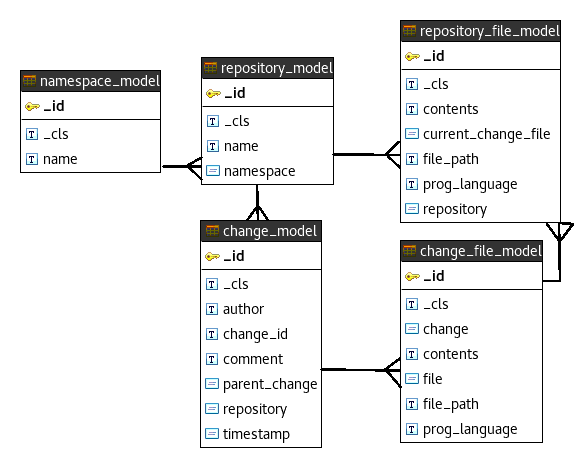
\includegraphics[width=0.75\textwidth]{Figures/nosql-db.png}
    \end{center}
  	\caption{Modelo de Base de Datos en MongoDB.}
    \label{nosql-db}
\end{figure}

El NamespaceModel solo consiste de:
\begin{itemize}
\item el nombre del Namespace
\item el ID que se genera por defecto
\end{itemize}
Esto representa los espacios donde usuarios y grupos pueden crear repositorios. Se considera que los Namespace deben existir de forma única.

El RepositoryModel representa un repositorio y tiene:
\begin{itemize}
\item un nombre
\item permanece a un Namespace
\item el ID que se genera por defecto
\end{itemize}
Cada par de Namespace y Repositorio debe ser una combinación única.

El próximo modelo, RepositoryFileModel, representa un archivo ubicado dentro de un repositorio. Sus atributos son:
\begin{itemize}
\item contenidos del archivo
\item el repositorio a que permanece
\item el lenguaje de programación para que el editor puede cambiar su comportamiento para el lenguaje específico
\item la ubicación del archivo dentro del repositorio incluyendo su nombre
\item un archivo de cambio que representa el estado actual y la última modificación realizada en el mismo, de lo cual se presenta más adelante.
\end{itemize}

El ChangeModel representa un cambio realizado en el repositorio, como los commits de Git. Tiene atributos como:
\begin{itemize}
\item una ID que se lo maneja la aplicación (que viene a ser un hash SHA1, inspirado por Git, de los contenidos y metadatos del mismo cambio)
\item un comentario
\item un autor
\item una estampa de tiempo que tiene tanto la hora como la fecha en que se realizó el cambio
\item el repositorio en que se hizo el cambio
\item una referencia al cambio anterior para que se puede construir una historial de cambios.
\end{itemize}

El ChangeFileModel es como el RepositoryFileModel en que representa archivos, pero en este caso son archivos modificados dentro de un cambio. Por lo tanto lleva los mismos atributos que RepositoryFile solo que en lugar de tener referencias a un repositorio directamente se referencia a un cambio realizado (el cual tiene metadatos como un comentario, autor, cambio previo y momento de modificación) y al archivo del repositorio que modifica (de esta forma puede modificar también la dirección de los archivos quienes no habría otra forma de buscarlos).

Finalmente el TemporaryChangeFileModel no se utiliza actualmente pero como los dos FileModels vistos anteriormente, esta lleva atributos básicos de un archivo. Originalmente se lo planteo para realizar una operación intermedio como la fase del Git Stage en donde se selecciona previo a un commit los cambios que van a estar incluidos dentro del mismo. Pero al final, aunque el modelo de datos esta para suportar varios archivos cambiados dentro de un solo cambio, no esta implementado así. Por temas de tiempo, retraso y alcance, se ha optado por llevar un mini control de versiones de cada archivo dentro de un repositorio, así que en realidad cada cambio en el repositorio solo refleja un archivo cambiado de forma independiente y no hay necesidad para la complejidad del paso intermedio que este modelo representa. 

\index{Controlar Versiones de Código}
\subsubsection{GitLab}
Al settings agregamos las siguientes lineas para configurar la conexión con GitLab:
\lstset{language=Python}
\begin{lstlisting}
GITLAB_DEFAULT_SERVER = '1'

GITLAB_SERVERS = {
    '1': {
        'WITH_TOKEN': True,
        'WITH_CRED': False,
        'API_PROTOCOL': 'http://',
        'API_PORT': '',  # por defecto:
                        # :22 para SSH,
                        # :443 para HTTPS,
                        # :80 para HTTP
        'HOST': '10.10.10.11',
        'SSH_PORT': 22,
        'HTTP_PORT': 80,
        'HTTPS_PORT': 443,
        'USER': "GitEDU",
        'PASSWORD': 'GitEDU2017',
        # expira el 31 de marzo 2018:
        'TOKEN': 'JqMzkgDNvhZ7ofdPa5z5',
        # nunca expira, pero el nivel de 
        # acceso es menor:
        # 'TOKEN': 'TrCfvrdsXzpLFETyc7Q5',  
    }
}
\end{lstlisting}
\lstset{language=Bash}

La conexión a la API de GitLab se realiza de la siguiente manera:
\lstset{language=Python}
\begin{lstlisting}
gitlab_default_srv = GITLAB_DEFAULT_SERVER


def connect_to_gitlab_token(protocol=None,
        host=None, port=None, token=None):
    if host is None:
        return None
    # gitlab_conn = gitlab.Gitlab(protocol
            + host + port, token)
    gitlab_conn = gitlab.Gitlab(protocol
            + host, token)
    #gitlab_conn.auth()
    return gitlab_conn


def connect_to_settings_gitlab_token(
        indx=GITLAB_DEFAULT_SERVER):
    return connect_to_gitlab_token(
            protocol=GITLAB_SERVERS
                [indx]['API_PROTOCOL'],
            host=GITLAB_SERVERS[indx]
                ['HOST'],
            port=GITLAB_SERVERS[indx]
                ['API_PROTOCOL'],
            token=GITLAB_SERVERS[indx]
                ['TOKEN'])


def connect_to_gitlab_user_password(protocol=None,
        host=None, port=None, user=None,
        password=None):
    if host is None:
        return None
    gitlab_conn = gitlab.Gitlab(protocol + host
            + port, email=user, password=password)
    gitlab_conn.auth()
    return gitlab_conn


def connect_to_settings_gitlab_user_password(
        indx=GITLAB_DEFAULT_SERVER):
    return connect_to_gitlab_user_password(
            protocol=GITLAB_SERVERS[indx]
                    ['API_PROTOCOL'],
            host=GITLAB_SERVERS[indx]['HOST'],
            port=GITLAB_SERVERS[indx]
                    ['API_PROTOCOL'],
            user=GITLAB_SERVERS[indx]['USER'],
            password=GITLAB_SERVERS[indx]
                    ['PASSWORD'])


def connect_to_settings_gitlab(
        indx=GITLAB_DEFAULT_SERVER):
    if GITLAB_SERVERS[indx]['WITH_TOKEN']:
        return connect_to_settings_gitlab_token(
                indx)
    elif GITLAB_SERVERS[indx]['WITH_CRED']:
        return connect_to_settings_gitlab_user_password(
                indx)
    else:
        return None

gitlab_srv = None
try:
    gitlab_srv = connect_to_settings_gitlab(
            gitlab_default_srv)
except Exception as e:
    print("No se pudo connectar a GitLab")
    print(e)
\end{lstlisting}
\lstset{language=Bash}

% TODO

\subsection{Aspectos Sociales}
Para temas de organización, se ha considerado que aquellos componentes de la aplicación que tienen que ver con interacción social deben existir independientemente de las funcionalidades principales del mismo aplicación. Es con este fin que los componentes del mismo se desarrollaron en un ''app'' distinto 'socialApp'' como fue creada previamente.

% TODO

%
% TODO if time
%\index{Sincronizar Notas por LTI}
%\subsection{Sincronizacion de Notas por LTI}
%

\subsection{API Externa}
% TODO

\index{Ejecutar Código}
\section{EduNube}

% TODO: Mandar como anexo:
% TODO: Solo resumir aqui

La gestión de dependencias del sistema EduNube se maneja con un entorno virtual y el gestor de paquetes de python pip. El siguiente es un script de bash diseñado a detectar si es que existe el entorno virtual (lo crea en caso de que no existe) y después instala los requerimientos faltantes como son especificados en un archivo aparte ''requirements.en.txt'' que da librerías y sus versiones.

\begin{lstlisting}
#! /usr/bin/head -n 2
# run with `source activate-en.sh`
PROJECT=en
ENV_DIR=env-$PROJECT
if [ ! -d $ENV_DIR ]; then
        virtualenv --python=python3 $ENV_DIR
fi
source $ENV_DIR/bin/activate
pip3 install -r requirements.$PROJECT.txt
\end{lstlisting}

El script anterior se ejecuta desde el raiz del repositorio con el comando:

\begin{lstlisting}
source activate-en.sh
\end{lstlisting}

Con el entorno creado y activado se puede proceder a instalar cualquier dependencia necesaria que no ha sido instalado previamente:

\begin{lstlisting}
pip3 install django==1.10.6 psycopg2==2.7.1 pymodm==0.4.0 ipython
\end{lstlisting}

Para el presente proyecto se instalaron las siguientes dependencias:
\begin{itemize}
	\item Django (1.10.6) como framework para el desarrollo del backend.
    \item Psycopg2 (2.7.1) como librería para conectarse a bases de datos PostgreSQL.
    \item ipython (6.1.0) como interprete interactivo de Python para hacer pruebas en el curso del desarrollo.
\end{itemize}

Con las dependencias instaladas o con cada cambio que se realiza de dependencias se ejecuta el siguiente comando para actualizar la lista de los mismos:

\begin{lstlisting}
pip freeze > requirements.txt
\end{lstlisting}

Se inicia el proyecto de Django con el comando:

\begin{lstlisting}
django-admin startproject EduNube
\end{lstlisting}

También antes de iniciar el desarrollo debe estar configurado el base de datos para ocupar el mismo. Primero es necesario crear y configurar un usuario y base de datos para ser ocupado:

\begin{lstlisting}
su - postgres
psql
\end{lstlisting}
\begin{lstlisting}
	postgres=# CREATE USER edunubeser WITH PASSWORD '3d?N_6E';
	postgres=# CREATE DATABASE edunubedb WITH OWNER edunubeser;
	postgres=# \q
psql edunubedb -U postgres
	edunubedb=# CREATE SCHEMA edunubeapp AUTHORIZATION edunubeser;
	edunubedb=# ALTER USER edunubeser SET search_path TO edunubeapp;
	edunubedb=# \q
psql edunubedb -U edunubeser
	edunubedb=> SELECT current_schema();
		Debe decir: edunubeapp
	edunubedb=> \q
\end{lstlisting}

Segundo, se abre el settings.py (dentro de la carpeta EduNube/EduNube) y se remplaza (para desarrollo, en producción debe llevar valores distintos) el atributo DATABASES con lo siguiente:
\lstset{language=Python}
\begin{lstlisting}
DATABASES = {
    'default': {
        'ENGINE': 'django.db.backends.postgresql_psycopg2',
        'NAME': 'edunubedb',
        'USER': 'edunubeser',
        'PASSWORD': '3d?N_6E',
        'HOST': '127.0.0.1',
        'PORT': '5432',
    }
}
\end{lstlisting}
\lstset{language=Bash}

Ahora se puede migrar las tablas iniciales de Django:
\begin{lstlisting}
cd EduNube
python manage.py makemigrations
python manage.py migrate
\end{lstlisting}

También creamos un superusuario de Django para temas administrativos:
\begin{lstlisting}
python manage.py createsuperuser
\end{lstlisting}

También se puede crear el app inicial (para lógica del editor de código):
\begin{lstlisting}
python manage.py startapp apiApp
\end{lstlisting}

Y de paso se lo agrega a INSTALLED\_APPS una linea 'apiApp' en el settings.py para que sus tablas definidos a futuro en models.py también se migran con los demás migraciones.

Para resolver un problema de zonas de tiempo, se ha desactivado esta característica de Django con el siguiente linea en el settings.py:
\lstset{language=Python}
\begin{lstlisting}
USE_TZ = False
\end{lstlisting}
\lstset{language=Bash}

Para crear la base de datos de MongoDB:
\begin{lstlisting}
mongo
\end{lstlisting}
\lstset{language=sql}
\begin{lstlisting}
use eduNubeDB
db.createUser(
    {
        user: "eduNubeUser",
        pwd: "3d?N_6E",
        roles: [ "readWrite", "dbAdmin" ]
    }
)
\end{lstlisting}
\lstset{language=Bash}

El mismo se define en el settings de la siguiente manera:
\lstset{language=Python}
\begin{lstlisting}
NOSQL_DATABASES = {
    'nosql': {
        'NAME': 'eduNubeDB',
        'USER': "eduNubeUser",
        'PASSWORD': '3d?N_6E',
        'HOST': '127.0.0.1',
        'PORT': '27017',
    }
}
\end{lstlisting}
\lstset{language=Bash}

\subsection{Autenticación}
El diseño planteado para el sistema EduNube propone dos tipos de autenticación:
\begin{itemize}
\item Clasica para usuarios humanas
\item Basada en Criptografía Asimétrica para ofrecer mayor seguridad y permitir integración con otros sistemas como GitEDU
\end{itemize}

\subsubsection{Autenticación Clasica}
Para la administración del sistema por operador humano se considera necesario la autenticación clásica mediante usuario y contraseña. Para la misma se ocuparon la misma implementación del framework Django y código reutilizado de GitEDU que tiene el mismo propósito.

\subsubsection{Autenticación basado en Criptografía Asimétrica}
Para ofrecer mayor seguridad al sistema de ejecución de código, EduNube, se considera más óptimo utilizar una sistema de autenticación basado en criptografía asimétrica de una manera similar a las llaves de SSH, donde el servidor tiene la oportunidad de conocer bien la identidad del cliente. Aunque no se ha logrado encontrar una implementación factible para la solución planteada, se considera como una solución utilizar una especie de API token similar a otros sistemas. Para generar el token, se ha logrado encontrar un estándar, JSON Web Tokens, que tiene la finalidad de ayudar al servidor identificar y verificar la validez de un cliente desconfiable mediante datos que el servidor mismo cifra con un tipo de llave privada.

A continuación se presenta la lógica para descifrar y cifrar los tokenes con el fin de generar/actualizarlo y también poderlo validar contra una tabla interna de la base de datos a lo que un cliente se lo envía:
\begin{lstlisting}
def decode_api_token(api_token=None):
    if api_token is None:
        raise ValueError("API_Token can't be None")
    return jwt.decode(api_token.token, api_token.secret_key,\
        algorithms=[api_token.token_algo])

def update_api_token(api_token=None, regen_secret_key=False):
    if api_token is None:
        raise ValueError("API_Token can't be None")
    if regen_secret_key or api_token.secret_key is None or\
            len(api_token.secret_key) == 0:
        api_token.secret_key = bcrypt.gensalt()
            # Generate Random Unique Secret_Key
    api_token.edit_date_in_token =\
        api_token.edit_date.__str__()
    payload = {
        'app_name': api_token.app_name,
        'created_date': api_token.created_date.__str__(),
        'edit_date': api_token.edit_date_in_token,
        'expires': api_token.expires
    }
    if api_token.expires:
        if api_token.expire_date is not None:
            payload['expire_date'] = api_token.expire_date
    api_token.token = jwt.encode(payload,\
        api_token.secret_key, algorithm='HS256')\
        # Generate Token
    api_token.save()
\end{lstlisting}

Como parte de la administración de este aspecto del sistema de autenticación, se encuentra implementado las funcionalidades de crear, actualizar, leer y borrar estos tokens de autenticación, siempre y cuando el usuario logueado tenga el permiso ''auth\_admin.manage\_tokens''. Si no se crea este permiso, como es el caso del ambiente de desarrollo, la política de Django es solo permitir cuentas de superusuario para acceder a estas vistas.

% <TODO>
\index{Ejecutar Código}
\subsection{Ejecución de Código en Linea}

% If Time
%\index{Calificar Código}
%\subsection{Calificación Automatizada con Pruebas Unitarias}

\subsection{API Externa}
% </TODO>

% Chapter 5

\chapter{Pruebas}
\label{capitulo5}

\section{Preperaciones del Ambiente de Pruebas}

\section{Plan de Pruebas}
La validación del presente trabajo de titulación se lo ha planteado en tres fases:
\begin{enumerate}
  \item Flujos completos de Funcionalidad
  \item Pruebas Funcionales
  \item Pruebas de Integración
\end{enumerate}
Donde se considera que estas mismas pruebas deben ser automatizados en el mayor parte posible con la finalidad de reducir variaciones que puede introducir un operador humano en aplicaciones distintas de una prueba.

\subsection{Flujos completos de Funcionalidad}
Estas pruebas son de alto nivel para revisar funcionalidad desde el punto del usuario en distintos roles de la aplicacion y llevar cada uno de esos roles por las distintas fases de su ciclo de vida dentro de la aplicacion. Se considera Selenium como buena opcion para la automatizacion de esta fase de pruebas.

\subsubsection{Administrador}
Dentro del ciclo de vida del administrador se debe probar:
\begin{enumerate}
  \item Creacion/Lectura/Actualizacion/Eliminacion de API Tokens en los sistemas respectivos que son:
  \begin{itemize}
    \item EduNube
    \item GitServerHTTPEndpoint
  \end{itemize}
  \item Registros de Plantillas Nuevas y Actualizacion de Plantillas Existentes de Virtualizacion
  \begin{itemize}
    \item La capacidad de establecer herencia de plantillas con el .repospec
    \item La capacidad de proteger archivos a traves del  .edunubeignore y el .edunubeignore.children
    \item La capacidad de incluir archivos de forma automatica en extenciones de la plantilla con el .templateinclude
  \end{itemize}
\end{enumerate}

\subsubsection{Profesor}
Dentro del ciclo de vida del profesor se debe probar:
\begin{enumerate}
  \item Extención de Plantillas de Virtualizacion
  \item Ejecutación de Plantillas de Virtualización
  \item Validación de las protecciones y herencia dado por los archivos de metadata en cada plantilla
\end{enumerate}

\subsubsection{Estudiante}
\begin{enumerate}
  \item Autenticación por LTI
  \item Editar Código en Línea
  \item Ejecutar Código en Línea
\end{enumerate}

\subsection{Pruebas Funcionales}
Estas pruebas son de baja nivel y van directamente contra funcionalidades del código. Se propone llevar las mismas con las pruebas unitarias que lleva Django como marco de desarrollo pero de esta misma forma así mismo se require que la pruebas no se llevan en más que un sistema a la véz y entonces en algunos casos no se podrá realizar pruebas completas de APIs de integración con otros sistemas, si no para las mismas se podria utilizar clientes que simulan la presencia del sistema consumidor externo o incluso refrencias cruzadas (como enlaces simbolicas de UNIX y submodulos de Git) para probar estas funcionalidades.

\subsubsection{GitEDU}
Para las pruebas de GitEDU, se necesita desabilitar ciertas funcionalidades de consumo de los dos servicios externos EduNube y GitServerHTTPEndpoint los cuales no se encuentran activos y levantados al momento de ejecutar estas pruebas con la necesidad de que estas pruebas de integración se los extrae a ser ejecutadas directamente con las pruebas unitarias de las respectivas sistemas.

\subsubsection{EduNube}
Las pruebas de EduNube deben llevar acabo validación de los entonos distintos de virtualización/ejecución de código atraves del API externa, el cliente estandar que utiliza GitEDU y el manejo adecuado de los API Tokens y .RepoSpec.

\subsubsection{GitServerHTTPEndpoint}
Las pruebas de GitServerHTTPEndpoint deben validar la API externa, manejo de API Tokens, cliente estandar que utiliza GitEDU y distinas operaciónes internas de Git que realiza el mismo sistema.

\subsection{Pruebas de Integracion}
Como parte de las pruebas unitarias del fase anterior, se debe validar que los mismos clientes que se ha probado son los que realmente esta utilizando cada sistema para con ello asegurar el cumplimiento de la integracion esperada. Realizando esta fase de esta forma podria permitir que se realiza al mismo rato de las pruebas unitarias de Django del fase anterior.

\section{Resultados}


% Chapter 6

\chapter{Despliegue}
\label{capitulo6}

\section{Plan de Despliegue}
En el curso del desarrollo, depuracion y ejecuccion de pruebas llegó a ser evidente en enorme consumo de recursos necesarios para levantar todos los servicios desarrollados y auxiliares a la vez, razon por el cual, se ha visto la necesidad de un rediseño de forma mas liviana de la manera en que se despliegue todos los componentes integrados a la aplicacion para con ello terminar las fases mencionadas anteriormente y dar paso a ejecuccion en ambientes de pocos recursos, tanto en el ambito de desarrollo como de produccion. En la implementacion original de la arquitectura fisica para el desarrollo, se habia planteado una colleccion de maquinas virtuales quienes representarian servidores distintas dentro de una red, pero para temas de optimizar recursos, se ha realizado los siguientes cambios los cuales se documentan a lo largo de este capitulo:
\begin{itemize}
	\item Kubernetes (backend de virtualizacion) se ubica en una maquina virtual de Xen (con paravirtualizacion activa para aumentar el rendimiento del sistema virtualizado) dado que el mismo, por temas de seguridad, debe seguir de una forma aislada. De esta forma se simula que esta en un servidor aparte, sea fisico o virtual (se recomienda mejor virtualizar todo el cluster final de Kubernetes en algun hipervisor de tipo 1 para garantizar mayor seguridad y aislamiento) pero sin la mayor parte de las perdidas de rendimiento que se dio con MiniKube (alojado en VirtualBox).
    \item Los servicios auxiliares en lugar de ser maquinas virtuales de Xen ahora son contenedores de Docker.
    \item Los servicios desarrollados se los han convertido en servicios (Systemd) del sistema operativo, no tanto por temas de rendimiento (aunque se podria mejorar el rendimiento de esta forma, asignandoles a un usuario con mayor prioridad de ejecuccion como el usuario root\footnote{Pero realizarlo esta afuera del alcance de este tesis, una solucion asi de software tampoco puede cambiar los recursos fisicos de la maquina.}\footnote{Nunca se debe asignar un servicio que se consume en la red externa a algun usuario con privilegios de superusuario, como root, ya que el mismo abre todo el sistema operativo a un nuevo vector de ataque por el mismo servicio. En este caso debe ser un nuevo usuario, preferiblemente uno por cada servicio, con acceso restingido que tiene mayor prioridad de ejecucion para sus procesos.}) si no por temas de facilitar la administracion del mismo.
    \item La integracion de los servicios con NGinX para que el mismo puede protegerlos y operar en la capacidad de proxy inversa, proxy de terminacion SSL/TLS, servidor de archivos estaticos y validador de peticiones sin mayor perdida de rendimiento.
\end{itemize}
% TODO
% diagrama de red/fisica

\section{Preperaciones del Ambiente de Despliegue}
Para preperar el ambiente de despliegue se lo ve pertinente planificar direcciones IP, dominios y puertos para los varios servicios que requieren ser levantados:
\begin{description}
	\item[Maquina Fisica] con Debian 9.x para Servicios y Docker: \textit{10.10.10.1}
    \begin{description}
    	\item[NGinX] \textit{http://0.0.0.0:80}
        \begin{itemize}
            \item \textit{http://10.10.10.1:80} \& \textit{http://git.localhost:80} -> GitWeb
            \item \textit{http://gitedu.localhost:80} -> GitEDU
            \item \textit{http://edunube.localhost:80} -> EduNube
            \item \textit{http://gitsrvendpoint.localhost:80} -> GitServerHTTPEndpoint
            \item \textit{http://gitlab.localhost:80} -> GitLab
            \item \textit{http://moodle.localhost:80} -> Moodle
        \end{itemize}
        \item[GitEDU] \textit{http://0.0.0.0:8000}
        \item[EduNube] \textit{http://0.0.0.0:8001}\footnote{Este puerto esta en conflicto con el Dashboard de Kubernetes, o se podria cambiar este puerto o montar el Dashboard de Kubernetes solo en la maquina virtual si es que fuera el caso}
        \item[GitServerHTTPEndpoint] \textit{http://0.0.0.0:8002}
        \item[Docker] \textit{10.10.10.1}
        \begin{description}
        	\item[MySQL] \textit{0.0.0.0:3306} -> \textit{moodledb:3306}
        	\item[Moodle] \textit{0.0.0.0:8201} -> \textit{moodle:80}
        	\item[GitLab CE] \textit{10.10.10.1}
            \begin{itemize}
            	\item \textit{0.0.0.0:8143} -> \textit{gitlab:443}
            	\item \textit{0.0.0.0:8101} -> \textit{gitlab:80}
            	\item \textit{0.0.0.0:8122} -> \textit{gitlab:22}
            \end{itemize}
        \end{description}
    \end{description}
    \item[Maquina Virtual (Xen)] con Debian 9.x para el Cluster (solo 1 nodo maestro) de Kubernetes: \textit{10.10.10.12}
\end{description}

\subsubsection{Moodle en Docker}
La instalacion de Moodle en Docker consiste de los siguientes pasos:
\begin{enumerate}
	\item Bajar el imagen de Docker oficial de MySQL:
    \begin{lstlisting}    
docker pull mysql
    \end{lstlisting}
    \item Bajar un imagen de Docker de Moodle:
    \begin{lstlisting}    
docker pull jauer/moodle
    \end{lstlisting}
    \item Ejecutar el imagen de MySQL en el fondo (-d) con un nombre idenficable (moodledb), paso de puertos (10.10.10.1:3306 -> moodledb:3306), un volumen de persistencia para el motor de base de datos, nombres de bases de datos, usuarios y contraseñas de MySQL y una peticion de que siempre se reinicia el contenedor a lo que muere con algun error:
    \begin{lstlisting}    
docker run -d --name moodledb -p 3306:3306 -v \
/srv/moodle/mysql:/var/lib/mysql -e \
MYSQL_DATABASE=moodle -e MYSQL_ROOT_PASSWORD=moodle \
-e MYSQL_USER=moodle -e MYSQL_PASSWORD=moodle \
--restart always mysql
    \end{lstlisting}
    \item Ejecutar el imagen de Moodle con opciones similares al anterior, con un enlace a la base de datos con un dominio local de DB, metadatos del url en que debe responder y ocupar el puerto 8201 local como puerto 80 del contenedor (un passthrough):
    \begin{lstlisting}    
docker run -d -P --name moodle --link moodledb:DB\
-e MOODLE_URL=http://10.10.10.1:8201 -p 8201:80 \
-v /srv/moodle/data:/var/moodledata \
--restart always jhardison/moodle
    \end{lstlisting}
    \item Y finalmente visitamos http://10.10.10.1:8201/ para terminar la instalacion inicial de Moodle y realizar su configuracion inicial.
\end{enumerate}

\subsubsection{GitLab en Docker}
Para instalar GitLab en Docker, se sigue pasos similares a los vistos previamente con Moodle:
% TODO: Cite
%https://hub.docker.com/r/gitlab/gitlab-ce/
%https://docs.gitlab.com/omnibus/docker/
\begin{enumerate}
	\item Bajar el imagen de Docker:
    \begin{lstlisting}    
docker pull gitlab/gitlab-ce
    \end{lstlisting}
    \item Ejecutar el imagen de Docker:
    \begin{lstlisting}    
docker run --detach --hostname 10.10.10.1 \
--publish 8143:443 --publish 8101:80 \
--publish 8122:22 --name gitlab --restart always \
--volume /srv/gitlab/config:/etc/gitlab \
--volume /srv/gitlab/logs:/var/log/gitlab \
--volume /srv/gitlab/data:/var/opt/gitlab \
gitlab/gitlab-ce:latest
    \end{lstlisting}
    \item Visitar http://10.10.10.1:8101/ para cambiar la contraseña de root
\end{enumerate}

\index{Hipervisor} \index{Virtualización} \index{Contenedor}
\subsubsection{Máquina Virtual de Xen}
Con el fin de proteger la maquina fisica contra usuarios finales, sean maliciosos o solo sin conocimientos adecuados, hay la necesidad de que el ambiente que ejecuta codigo sea aislado con virtualizacion. Pero el rendimiento de esta maquina virtual necesita ser maximizada para poder permitir su uso con un minimo de recursos. Es, por lo tanto, que se ha propuesta utilizar una maquina virtual de Xen de baja nivel con mejores de rendimiento con la tecnologia de paravirtualizacion con la finalidad de que esta misma logra ofrecer alta aislamiento, y por lo tanto seguridad, frente una alta rendimiento.

\paragraph{Construción de Servidor Virtualizado para Cluster de Kubernetes}
Las caracteristicas minimas que pide Kubernetes para su nodo maestro son 2 nucleos y 2 GiB de RAM, es por aquello razon que se crea una maquina virtual paravirtualizada con estas mismas caracteristicas. En el curso del año que se ha trabajado este trabajo de titulacion la comunidad de Debian se ha logrado arreglar  el bug que antes causó problemas la ultima vez que se realizó una maquina virtual nueva de Debian 9 y es con este motivo que se puede crear una maquina virtual nueva sin ninguna necesidad para pasos adicionales:
\begin{lstlisting}
xen-create-image --hostname=debian-k8s-master \
--ip=10.10.10.12 --netmask=255.255.255.0 \
--gateway=10.10.10.1 --memory=2048mb --vcpus=2 \
--lvm=Xephyr-VG --pygrub --dist=stretch --force \
--size=10240mb --swap=1024mb
\end{lstlisting}
% TODO:
% see Screenshot_2017-12-29_15-21-49.png

\paragraph{Instalación de Docker}
Para utilizar Kubernetes dentro de esta maquina virtual es necesario primero contarnos con una instalacion de Docker. Kubernetes no garantiza que va a funcionar con las ultimas versiones de Docker ya que el API de Docker cambia constantemente, especialmente con actualizaciones de seguridad, pero de esta misma forma para la seguridad de la misma, queremos contar con la misma forma estable. Se instala de la siguiente manera en Debian (para otros sistemas operativos, a lo mucho solo se tendria que cambiar el gestor de paquetes apt por el respectivo de su sistema):
\begin{enumerate}
	\item Actualizar el sistema operativo
    \begin{lstlisting}
apt update
apt upgrade
    \end{lstlisting}
    \item Instalar curl si es que no esta instalado previamente
    \begin{lstlisting}
apt install curl
    \end{lstlisting}
    \item Bajar el instalador actual de Docker
    \begin{lstlisting}
curl -fsSL get.docker.com -o get-docker.sh
    \end{lstlisting}
    \item Ejecutar el instalador de Docker
    \begin{lstlisting}
sh get-docker.sh
    \end{lstlisting}
\end{enumerate}
% TODO: see Screenshot_2017-12-29_15-31-49.png

\paragraph{Instalación de Cluster de Kubernetes}
% TODO: Cite
%https://kubernetes.io/docs/setup/independent/install-kubeadm/
Para instalar el cluster de Kubernetes, el proceso es relativamente sencillo con una harramienta que se llama \texttt{kubeadm} que se encarga de levantar, gestionar y bajar nodos del cluster. Primero para instalar el mismo:
\begin{enumerate}
	\item Debemos tener suporte en el gestor de paquetes APT para el protocolo HTTPS:
    \begin{lstlisting}
apt update && apt install -y apt-transport-https
    \end{lstlisting}	
	\item Agregamos el repositorio de Kubernetes para Debian y Ubuntu:
    \begin{lstlisting}
curl -s \
	https://packages.cloud.google.com/apt/doc/apt-key.gpg \
	| apt-key add -
cat <<EOF >/etc/apt/sources.list.d/kubernetes.list
deb http://apt.kubernetes.io/ kubernetes-xenial main
EOF
    \end{lstlisting}
    \item Actualizamos los indices de APT y procedemos a instalar:
    \begin{lstlisting}
apt-get update
apt-get install -y kubelet kubeadm kubectl
    \end{lstlisting}
\end{enumerate}

% TODO: Cite 
%https://kubernetes.io/docs/setup/independent/create-cluster-kubeadm/
El levantamiento de un nodo maestro basica se puede hacer con el commando:
    \begin{lstlisting}
kubeadm init
    \end{lstlisting}
Que utiliza todos los valores por defecto, pero Kubernetes requiere para su funcionamiento algun driver de red de los cuales se ha elegido Flannel ya que es el más sencillo y no necesitamos mayor funcionalidad como Switches programables, ni enrutamiento o ACLs en las redes de nuestro cluster debido a que no se busca levantar sistemas de produccion aqui, solo contendores independientes y obviamente otros drivers de red con mayor funcionalidad tienen un costo de rendimiento mayor. Si es que se levanto el cluster con el comando anterior, se lo puede destruir con el siguiente commando: 
    \begin{lstlisting}
kubeadm reset
    \end{lstlisting}
Ya que Flannel requiere que se define el rango de IPs con que se trabajara el cluster como 10.244.0.0/16\footnote{Si, parece que tiene que ser exactamente este rango y no suporta mas que $65,536$ contenedores al mismo tiempo, pero eso debe ser suficiente para el proposito actual.}, por lo tanto en realidad, para trabajar con Flannel es necesario agregar un argumento al commando de levantamiento del cluster como se lo indica a continuacion:
    \begin{lstlisting}
kubeadm init --pod-network-cidr=10.244.0.0/16
    \end{lstlisting}
Esto se genera una salida como la que se demuestra a continuacion:
    \begin{lstlisting}
To start using your cluster, you need to run the following(...)
as a regular user:

  mkdir -p $HOME/.kube
  sudo cp -i /etc/kubernetes/admin.conf $HOME/.kube/config
  sudo chown $(id -u):$(id -g) $HOME/.kube/config

You should now deploy a pod network to the cluster.
Run "kubectl apply -f [podnetwork].yaml" with one of the(...)
options listed at:
  https://kubernetes.io/docs/concepts/cluster-(...)
  administration/addons/

You can now join any number of machines by running the (...)
following on each node
as root:

  kubeadm join --token 655cb5.2275aa7df206fe69 \
  10.10.10.12:6443 --discovery-token-ca-cert-hash \
  sha256:4919df120063c4535fd03e909ce11dfe9e6448f8a7\
  67be914e86b16660d267c8
    \end{lstlisting}

Por defecto Kubernetes no permite que el nodo maestro aloje contenedores como una politica de seguridad, pero en este caso se quiere levantar un cluster de un solo nodo y por lo tanto se requiere cambiar esta politica con el siguiente commando:
    \begin{lstlisting}
KUBECONFIG=/etc/kubernetes/admin.conf kubectl taint nodes \
--all node-role.kubernetes.io/master-
    \end{lstlisting}
El Variable de Entorno de KUBECONFIG da el archivo que se ve a continuacion que autentica el cliente con el cluster. Una vez que se configura bien el cliente, este mismo deja de ser necesario. Entonces a continuacion para configurar el cliente:
    \begin{lstlisting}
mkdir -p $HOME/.kube
cp -i /etc/kubernetes/admin.conf $HOME/.kube/config
chown $(id -u):$(id -g) $HOME/.kube/config
    \end{lstlisting}

Se puede probar la conexion pidiendo la version del cliente y del servidor:
\begin{lstlisting}
kubectl version
\end{lstlisting}

% TODO: Cite
%#https://kubernetes.io/docs/concepts/cluster-administration/networking/
%https://kubernetes.io/docs/setup/independent/create-cluster-kubeadm/
Para instalar el driver de red Flannel (que es necesaria cualquier driver de red para Kubernetes previo a funcionamiento -- no se instala con ningun por defecto para que sea al eleccion del administrador quien instala ya que un cluster de Kubernetes solo puede ocupar un driver de red a la vez):
\begin{lstlisting}
sysctl net.bridge.bridge-nf-call-iptables=1
cat sysctl.conf
cat >> /etc/sysctl.conf << EOF

# For Kubernetes Flannel
net.bridge.bridge-nf-call-iptables = 1

EOF
kubectl apply -f \
https://raw.githubusercontent.com/coreos/flannel/v0.9.1/\
Documentation/kube-flannel.yml
\end{lstlisting}

A continuacion se puede validar que Flannel o cualquier driver de red para Kubernetes esta funcionando con el commando:
\begin{lstlisting}
kubectl get pods --all-namespaces
\end{lstlisting}
Y que se revisa en la salida del mismo si se logra levantarse \texttt{kube-dns} con una linea similar a:
\begin{lstlisting}
kube-system   kube-dns-...-...  3/3   Running  ... ...
\end{lstlisting}

Para utilizar volumenes de Git dentro del cluster, es necesario installar git en cada nodo:
\begin{lstlisting}
apt install git
\end{lstlisting}

Para consumir el cluster desde el servicio de EduNube, es necesario copiar el archivo /etc/kubernetes/admin.conf al otro equipo. Para realizar la copia, lo que mas conviene, especialmente en redes no tan confiables (ya que el admin.conf contiene los credenciales de superusuario de Kubernetes), es realizar la copia sobre SSH. Primero para validar la existencia de sshd:
\begin{lstlisting}
apt install net-tools
netstat -tupln
\end{lstlisting}
Se puede buscar un servicio llamado sshd que normalmente escucha en el puerto 22 (pero puede ser configurado en otro puerto para ofrecer un poco mas de seguridad\footnote{Normalmente un cambio de puerto no ofrece mayor seguridad y es mal consejo, pero en la experiencia del autor, la mayoria de ataques de fuerza bruta de SSH no utilizan ningun escaneo de puertos ya que son script kiddies o bots bien basicos}). Si es que no existe, hay que instalar el servicio:
\begin{lstlisting}
apt install openssh-server
\end{lstlisting}
Pero en la instalacion que realiza xen-tools se instala sshd por defecto. Dentro del servidor de Kubernetes no se tiene acceso al admin.conf cualquier usuario, entonces se require connectar por SSH como root, algo que normalmente es muy peligroso y se desabilita por defecto. Para permitirlo, hay que editar \texttt{/etc/ssh/sshd\_config} y reiniciar el servicio:
\begin{lstlisting}
vim.tiny /etc/ssh/sshd_config

# Editar la linea que diga PermitRootLogin para que diga:
PermitRootLogin yes

systemctl restart sshd
\end{lstlisting}

Desde el equipo que tiene EduNube como servicio se realiza la copia por SSH:
\begin{lstlisting}
scp root@10.10.10.12:/etc/kubernetes/admin.conf .
\end{lstlisting}
Se puede probar que funcionan los credenciales copiados con una peticion a Kubernetes de una lista de las maquinas que componen el cluster:
\begin{lstlisting}
kubectl --kubeconfig ./admin.conf get nodes
\end{lstlisting}
Si es que funcionan los crendenciales y el sistema que aloja el nodo maestro de Kubernetes esta expuesto a alguna red donde no hay sufficiente confianza para dejar que se connecta root por SSH, ya se puede deshabilitar la configuracion que se realizo anteriormente y reiniciar el servicio.

Para instalar los credenciales de Kubernetes para que EduNube tiene acceso (pero sin perderse los credenciales al MiniKube instalado anteriormente) se realiza los siguientes commandos:
\begin{lstlisting}
mv admin.conf ~/.kube/config.xen
cp ~/.kube/config ~/.kube/config.minikube
cp ~/.kube/config.xen ~/.kube/config
\end{lstlisting}

Para validar que los credenciales se instalaron correctamente:
\begin{lstlisting}
kubectl version
\end{lstlisting}

\subparagraph{Validación de Cluster de Kubernetes}
Para validar el cluster de Kubernetes se puede entrar a la carpeta kubernetes dentro del repositorio de GitEDU/EduNube y realizar las siguientes validaciones del nuevo cluster:
\begin{lstlisting}
cd kubernetes/
kubectl create -f debian-pod.yaml
kubectl get pods/utility
kubectl describe pods/utility
kubectl create -f debian-pod-2.yaml
for manifest in `ls *.json`; do
    kubectl create -f $manifest;
done
kubectl get jobs
# no todos tendran exito al ejecutarse, algunos
# trabajos requieren configuraciones especiales
# que solo se encontraron en el entorno de
# expirimentos, y algunos de los expirimentos
# no fueron exitosos
watch -n 15 "kubectl get jobs"
# en este caso el primero en terminar:
kubectl describe jobs/pi
# El pod que fue creado (sera diferente):
# pi-kf8zv
kubectl describe pods/pi-kf8zv
# Ver la salida del trabajo
kubectl logs jobs/pi
\end{lstlisting}

% TODO: under consideration if time
%\paragraph{Interfaz de Administracion}
%kubectl apply -f https://raw.githubusercontent.com/kubernetes/dashboard/master/src/deploy/recommended/kubernetes-dashboard.yaml
%kubectl proxy -> will fail if executed at the same time as EduNube (port 8001)
\index{Contenedor} \index{Virtualización} \index{Hipervisor}

\section{Despliegue}
% TODO:
% servicios y su asignacion de puertos
% GitEDU - 8000/HTTP = gitedu.localhost
% EduNube - 8001/HTTP = edunube.localhost
% GitServerHTTPEndpoint - 8002/HTTP = gitsrvendpoint.localhost
% aux services (redir NGinX):
%		http://git.localhost:80 -> GitWeb
%		http://gitedu.localhost:80 -> GitEDU
%		http://edunube.localhost:80 -> EduNube
%		http://gitsrvendpoint.localhost:80 -> GitServerHTTPEndpoint
%		http://gitlab.localhost:80 -> GitLab
%		http://moodle.localhost:80 -> Moodle

\subsection{GitEDU}

\subsection{EduNube}

\subsection{GitServerHTTPEndpoint}

\section{Pruebas del Despliegue y Resultados}


% Chapter 7

\chapter{Conclusiones}
\label{capitulo7}

\section{Resultados}
% TODO: Resultados %% REVIEW
El principal resultado obtenido es el realizar un prototipo de la plataforma propuesta donde se integra tres servicios cuyas funcionalidades esenciales son:
\begin{description}
	\item[GitEDU,] ofrece una autenticación clásica y autenticación de LTI, manejo de namespace y repositorios. Adicionalmente cuenta con un editor de código en línea para gestionar archivos dentro de un repositorio, esto, llevado bajo un sistema de control de versiones interno.
    \item[EduNube,] mediante su API, ofrece toda la funcionalidad necesaria para que cada uno de los usuarios de GitEDU pueda ejecutar el código que desarrolló dentro de la plataforma. El servicio está planteado para extenderse con nuevas funcionalidades a futuro, por ejemplo el dar soporte a la ejecución de más lenguajes de programación (mediante contenedores de Docker), y la calificacion del código escrito por los usuarios.
    \item[GitServerHTTPEndpoint,] mediante su API, permite que los cambios realizados en el editor de GitEDU sean persistentes en repositorios de Git externos para su consumo por parte de aplicaciones y usuarios externos.
\end{description}

% TODO: get input on conclusions (are they okay for the thesis) %% REVIEW
% Minimo 1 Conclusion frente cada Objetivo Especifico
% Minimo 1 Conclusion frente cada Linea Problematica
% Lo que no va en resultados, puede ir a conclusiones
% Conclusiones tienen que ser declaraciones positivas o negativas, no van preguntas
% Cuantas Conclusiones poner? 3-5 es acceptable -> 7 conclusiones suele ser demaciado
% Tipicamente un recomendacion por cada cada conclusion

\section{Conclusiones}
A lo largo del desarrollo de este trabajo de titulación, se ha llegado a las siguientes conclusiones:

\begin{itemize}
  \item En base a la investigación de trabajos relacionados se puede proyectar que el sistema prototipo desarollado podría convertirse en una herramienta valiosa para la docencia de la Universidad Técnica Particular de Loja, con la finalidad de enseñar y evaluar a los estudiantes de programación. Y por lo tanto el prototipo realizado es el primer paso para cumplir con esta finalidad, pero para ello se requiere de un mayor trabajo a futuro.
  \item Para el desarrollo de sistemas educativos, LTI puede ser una buena solución a tomar en cuenta, para facilitar el flujo de autenticación entre diferentes sistemas de aprendizaje y enseñanza.
  %\item El servicio del editor de codigo en linea, ''GitEDU'', dispone de una interfaz web llamativa y funcional gracias a una potente combinacion de jQuery, AJAX, plantillas predefinidas de Bootstrap, XTerm.js y Ace Code Editor. % y la implementacion del mismo
  %forman una combinación potente para definir,
  %sin mayor esfuerzo, la interfaz adecuada para programar y ejecutar código en linea, y que el mismo tenga un alto nivel de funcionalidad.
  %\item Un sistema que viene a ser frontend para usuarios finales, como un editor de codigo debe poner bastante desempeño en tratar de ser llamativo y funcional ya que muchos usuarios solo se fijan en la aparencia y no en la funcionalidad que esta por detras, aunque si se dan cuenta eventualmente si falta funcionalidad. Por lo tanto es importante encontrar las herramientas adecuadas para que el editor de código en la plataforma sea tanto llamativa como funcional, porque la primera impresión es lo que más cuenta.
  \item Kubernetes y Docker son herramientas muy potentes y fáciles de implementar en soluciones de mayor complejidad para generar entornos confiables, construir sistemas de producción escalables y portables, así como para ejecutar trabajos por lotes con mayor grado de seguridad y con un alto rendimiento. Estas tecnologías permitieron cumplir con los requerimientos del servicio de EduNube que se encarga de ejecutar el código de usuarios finales.
  \item Para la implementación de control de versiones externo en el presente proyecto se ha concluido que cualquier servidor de Git es altamente pesado, especialmente GitLab que en su estado pasivo consume muchos recursos, y también GitWeb que tiene inconvenientes cada vez que recibe nuevos objetos de Git sobre HTTP.
  \item Para los datos que no bien estructurados o con campos de longitud altamente variable, como en el caso del código escrito por los estudiantes, las bases de datos no-relacionales como MongoDB, son una buena alternativa frente a las bases de datos relacionales además de simplificar el proceso. 
  \item Es importante que el interfaz de un sistema que se expone frente a los usuarios finales, en este caso, el editor de código en linea, ''GitEDU'', dispone de un fuerte combinación de tecnologías para obtener una interfaz llamativa y funcional en base a jQuery, AJAX, Bootstrap, XTerm.js y Ace Code Editor.
  \item Django/Python orientado a objetos permite desarollar con mayor rapidez, mayor enfoques a DRY y la extensibilidad del codigo a futuro. 
  \item La combinacion de Python 3 con librerias selecionadas para realizar los respectivos backends, es decir Django, PyModm, Bcrypt, PyJWT, Requests y ipython forman una combinación potente para el desarollo rápido de servicios de producción siempre y cuando se maneje de forma adecuada el diseño de los mismos y el manejo de distintos tipos de datos.
\end{itemize}


% Previously Chapter 8: Recomendaciones, united with Chapter 7: Conclusiones by recomendation of Ing. Maria del Carmen
%\chapter{Recommendaciones}
\section{Recomendaciones}
%\label{capitulo8}
% TODO: revisar si recomendations son adecuadas %% REVIEW
%Tipicamente un recomendacion por cada cada conclusion

En base a lo que se ha aprendido en el camino de este trabajo de titulación, se puede realizar las siguientes recomendaciones:

\begin{itemize}
  \item Cuando se desarrolla sistemas con un enfoque educativo, se recomienda reutilizar una implementacion de LTI para evitar problemas de integración con el software nuevo que se desarrolla.
  \item En el curso de realizacion de interfaces web, se recomiendo reutilizar el trabajo de terceros siempre y cuando hay la posibilidad, con el fin de poder dar mayor enfoque a la funcionalidad del backend.
  \item Para trabajar con cualquier base de datos, sea relacional o no relacional, lo más recomendable es trabajar con un ORM que permite abstraer la base de datos y facilitar el desarrollo y persistencia de datos en la misma. PyMODM es un ORM potente para combinar el poder de Python con MongoDB y un API bastante similar al ORM de Django.
  \item Siempre se recomienda utilizar nuevas tecnologias como Kubernetes, los cuales pueden ser utiles para resolver problemas actuales ya que ofrecen nuevas perspectivas y soluciones de los cuales no se los ha podido considerar antes.
  \item Donde hay posibilidad, se recomienda no trabajar con GitLab, a menos de que dispone de los recursos necesarios para ello y tambien que requiere las características avanzadas del mismo. En entornos donde sea posible, lo más recomendable es trabajar con Git sobre SSH, que además de ser más seguro, tiene mayor soporte por parte de Git y mayor inteligencia para la sincronización cuando se trabaja con este protocolo que puede dar como resultado mayor eficiencia en uso de red.
\end{itemize}

% TODO: escribir recomendacion general?

\section{Trabajos Futuros}
Se considera los siguientes aspectos que se podrian y/o se deben trabajar a futuro, los cuales no esta en ningun orden especifico:
\begin{itemize}
	\item Arreglar Errores en la funcionalidad existente, por ejemplo:
    \begin{itemize}
    	\item EduNube no actualiza de forma adecuada repositorios de ejecuccion, lo cual resulta muchas veces en la ejecuccion de una version antigua del mismo.
        \item EduNube no genera IDs de ejecuccion de forma adecuada.
    \end{itemize}
    \item Autenticacion en GitEDU y/o otros servicios mediante LDAP.
    \item Sincronizacion en tiempo real de codigo editado en GitEDU y sus respectivo backends de codigo, tal ves mediante websockets.
    \item Socializacion de vistas para editar codigo (GitEDU) con la finalidad de promover interaccion y collaboracion entre usuarios sobre los mismos.
    \item Un sistema de permisos para el editor de codigo (GitEDU).
    \item Distintas formas de calificacion, incluyendo:
    \begin{itemize}
    	\item Calificacion Manual por parte de professores.
        \item Calificacion Automatizado por parte del sistema (tal vez en forma de un servicio nuevo?) en base a pruebas unitarias definidos por professores.
        \item Calificacion Hibrida que combina los anteriores.
    \end{itemize}
    \item Sincronizacion de Notas (generados por la(s) modalidad(es) de calificacion anteriores) por LTI con los sistemas adecuadas para el manejo de los mismos, por ejemplo los LMS.
    \item Mas backends de Git para el servicio GitServerHTTPEndpoint, como por ejemplo GitLab o Djacket.
    \item Mas backends de persistencia de codigo para el servicio GitEDU como Redis o GitLab.
    \item Mas backends de virtualizacion para EduNube como OpenStack, Docker, etc.
    \item Versionamiento de APIs en todos los servicios.
    \item Auditoria de Seguridad del Sistema Desarrollado, especialmente en el caso de los APIs que no manejan estados y solo se protegen con API tokens JWT y a lo mucho TLS.
    \item Mejor gestion de la configuracion, actualmente hay componentes de algunos servicios que dejen de funcionar o que funcionan de forma inadecuada cuando no disponen de sus servicios dependientes. Debe ser configurable cuales servicios existen o no, dinamico la manera en que se encuentran y cada servicio tolerante a fallos en los demas servicios.
    \item Convertir los servicios en imagenes de Docker para montarlos mismos en un cluster de Kubernetes y realizar un estudio de alta disponabilidad/escalabilidad.
    \item Implementar el sistema de plantillas de GitEDU.
    \item Migrar servicios a Django 2.x (la proxima version de soporte a largo plazo de Django esta planificado como el 2.3) ya que en realizar esta migracion de version, actualmente se rompe la forma en que se llevan los URIs con un namespace para cada app.
    \item Automatizar y aumentar las pruebas unitarias de la aplicacion de acuerdo con el plan de pruebas original.
    \item Uso bidireccional del Git (por el momento es unidireccional, GitEDU solo guarda en los repositorios de GitWeb, nunca recupera codigo de usuarios guardado alli, que obviamente a futuro podria dificulta la interaccion entre el usuario y el sistema, en obligarle a siempre editar proyectos dentro del plataforma).
    \item Mayor soporte para caracteristicas de Git como ramas, tags, etc.
    \item Llevar metadatos de lenguaje de programacion / ejecutor seleccionado para repositorios en GitEDU, para su uso al momento de llamar al API de EduNube, se puede realizar la llamada adecuada (actualmente esta quemada el uso del ejecutor de Python 3).
    \item Recolleccion de datos para apoyar la toma de decisiones estrategicas.
\end{itemize}


%----------------------------------------------------------------------------------------
%	THESIS CONTENT - APPENDICES
%----------------------------------------------------------------------------------------

\appendix % Cue to tell LaTeX that the following "chapters" are Appendices

% Include the appendices of the thesis as separate files from the Appendices folder
% Uncomment the lines as you write the Appendices


% Appendix A - Vision Document

\chapter{Documento de Visión}
\label{visionDoc}
\label{AnexoA}

\section{Propósito}
Ayudar a mejorar los métodos de enseñanza que ofrece la Universidad Técnica Particular de Loja en cuanto a la programación y uso de base de datos para las carreras de Sistemas y Electrónica.
\paragraph{Alcance}
Se propone un sistema de edición de código en línea que a su vez integra LMS externos (para autenticación y notas), un servidor de control de versiones externo (para la persistencia de código), y un servicio web de ejecución de código en línea de una forma segura, eficaz y eficiente (para dar un ambiente de ejecución y pruebas tanto para los usuarios del sistema como para calificar de una forma automática).
\section{Definiciones, Acrónimos y Abreviaciones}
\begin{description}
	\item[LMS] Learning Management System (Sistema de Gestión de Aprendizaje)
    \item[LTI] Learning Tools Interoperability (estandar de Interoperabilidad entre Herramientas de Aprendizaje)
    \item[GitEDU] sistema de Git EDUcation
\end{description}
\subsection{Posición y Oportunidad de Negocios}
Con el avance continuo de la tecnología y su introducción en mas aspectos de la vida diaria, hay una necesidad creciente de ingenieros en sistemas y electrónica que puedan programar y entender el software que hace todo funcionar en adición a las bases de datos que están por detrás de estos mismos sistemas.
 
Es por aquella razón que ahora está de moda ofrecer plataformas en línea para la enseñanza dinámica de la programación. GitEDU espere ofrecer las mismas funcionalidades a un costo institucional menor a través de la integración con sistemas existentes e innovación para proveer una mejor experiencia de usuario, tanto estudiantes como profesores y llevar a cabo un mejor proceso de aprendizaje.

%\pagebreak
%\paragraph{Definición de Problema}
\begin{table}[h!]
  \begin{tabular}{|p{0.2\textwidth}|p{0.7\textwidth}|}
    \hline
    El problema de & enseñar y evaluar programación \\
    \hline
    afecta a & los estudiantes y docentes de las carreras de Sistemas y Electrónica \\
    \hline
    el impacto de lo cual es & el uso ineficiente de recursos universitarios en la enseñanza de la programación \\
    \hline
    Una solución exitosa seria & una aplicación web que ofrezca un editor de código en línea, la capacidad de ejecutar este código para proveer mejor interacción con los estudiantes, la capacidad de ejecutar pruebas unitarias para automatizar el proceso de calificaciones, la persistencia de código en un repositorio de control de versiones remoto para la fácil revisión de profesores y estudiantes, y la integración transparente con sistemas de gestión de aprendizaje externos para la autenticación de usuarios y la respectivo registro de notas. \\
    \hline
  \end{tabular}
  \caption{Definición del Problema.}
  \label{def-prob}
\end{table}

%\pagebreak
%\paragraph{Posición de Producto}
\begin{table}[h!]
  \begin{tabular}{|p{0.2\textwidth}|p{0.7\textwidth}|}
    \hline
    Para & docentes y estudiantes de la Universidad Técnica Particular de Loja \\
    \hline
    Quienes & tienen dificultades en la enseñanza y aprendizaje con la programación \\
    \hline
    GitEDU & es una plataforma web \\
    \hline
    Que & provee un espacio para la interacción entre profesores y alumnos para la enseñanza y aprendizaje de la programación y uso de las bases de datos \\
    \hline
    A diferencia de & otras plataformas altamente costosas que no se integran completamente con sistemas existentes de la universidad ni permiten alta interacción entre docentes y alumnos \\
    \hline
    Nuestro producto & da mayor capacidad para interacción entre estudiantes y sus docentes y se integra bien con las sistemas existentes para dar una mejor experiencia a todos los involucrados a un costo menor. \\
    \hline
  \end{tabular}
  \caption{Posición de Producto.}
  \label{pos-prod}
\end{table}

\pagebreak

\section{Usuarios e Interesados}
\subsection{Demográfica del Mercado}
En el año 2011, la Universidad Técnica Particular de Loja contaba con aproximadamente 4000 estudiantes presenciales y 24000 estudiantes a distancia con una tendencia creciente [UTPL-Datos-Estadisticos]. En la experiencia personal del autor, las carreras de Sistemas y Electrónica, por lo menos en la modalidad presencial, juntos representan aproximadamente un 10\% de todos los estudiantes en la universidad lo cual daría un mercado de estudiantes afectados por un nuevo sistema de aproximadamente un mínimo 2800 estudiantes. Según el directorio de docentes de la universidad, son 60 profesores en el departamento de Ciencias de la Computación y Electrónica [UTPL-Directorio-Docentes]. Con eso se puede estimar un mínimo de 2860 usuarios lo los cuales el sistema propuesto podría llegar a afectar.

Es precisamente la parte de la población, de usuario potenciales mencionado anteriormente, que está en el proceso de enseñar, evaluar y aprender habilidades de programación y consultar bases de datos que forman la base de usuarios de la aplicación.

%\pagebreak
%\paragraph{Resumen de Interesados}
%\begin{table}[h!]
  %\begin{tabular}{|p{0.15\textwidth}|p{0.35\textwidth}|p{0.4\textwidth}|}
% TODO: Caption before longtable, not after %% AESTHETICS
\begin{longtable}{|p{0.2\textwidth}|p{0.35\textwidth}|p{0.35\textwidth}|}
  \hline
  \textbf{Nombre} & \textbf{Descripción} & \textbf{Responsabilidades} \\
  \hline
  \endhead
  Analista & Trabaja con el Asesor Principal y Auxiliar para entender bien las necesidades institucionales para poder llevar un buen ingeniería de requerimientos y diseño del sistema propuesto. & Definir bien el problema para analizarlo, generar requerimientos en base a las necesidades para diseñar y documentar componentes del sistema final para el beneficio del Arquitecto de Software, Programador, Gestor de Proyecto y futuro mano de obra en el proyecto. \\
  \hline
  Arquitecto de Software & Trabaja con el Asesor Principal y Auxiliar para definir una arquitectura que garantiza que se cumpla con los atributos de calidad que requiere el sistema y será compatible con la infraestructura y sistemas institucionales ya existentes. & Diseñar los modelos de interacción entre todos los componentes internos y externos del sistema para con ello lograr un flujo eficaz y eficiente, que también cumple con los parámetros de los requerimientos no funcionales, en el sistema final. \\
  \hline
  Gestor de Proyecto & Trabaja con el Asesor Principal y Auxiliar para evaluar, estimar y establecer el alcance, los recursos y el cronograma del proyecto. & Distribuir de manera eficiente y eficaz los recursos para ayudar el analista, arquitecto de software, programador y administrador de sistemas y bases de datos cumplir dentro de los recursos, alcance y cronograma preestablecido. \\
  \hline
  Programador & Trabaja con el Asesor Principal, Asesor Auxiliar, y Analista para implementar soluciones técnicas que cumplen con el diseño dado por el analista. & Desarrollar el sistema en todos sus componentes. \\
  \hline
  Administrador de Sistemas y Bases de Datos & Trabaja con el Asesor Principal y Auxiliar para desplegar la aplicación en la institución. & El despliegue correcto del sistema con todos sus componentes en la institución respectivo. \\
  \hline
  Asesor Principal & Trabaja con el Asesor Auxiliar para poder aconsejar de la mejor manera el Analista, Arquitecto de Software, Gestor de Proyecto, Programador y Administrador de Sistemas y Bases de Datos. & La definición de necesidades y aprobación del producto final. \\
  \hline
  Asesor Auxiliar & Trabaja con el Asesor Principal para poder aconsejar de la mejor manera al Analista, Arquitecto de Software, Gestor de Proyecto, Programador y Administrador de Sistemas y Bases de Datos. & La definición de necesidades y aprobación del producto final. \\
  \hline
  Asesor de Documentación & Trabaja con el Analista y Gestor de Proyecto para asegurar la calidad de la documentación que se genera a lo largo del proyecto y que se cumple con el cronograma establecido entre el gestor del proyecto y los asesores principales y auxiliares. & La aprobación de los avances en la documentación y la documentación completa al final del proyecto. \\
  \hline
  %\end{tabular}
  \caption{Resumen de Interesados.}
  \label{res-inter}
\end{longtable}
%\end{table}

%\pagebreak
%\paragraph{Posición de Producto}
\begin{table}[h!]
  \begin{tabular}{|p{0.225\textwidth}|p{0.225\textwidth}|p{0.225\textwidth}|p{0.225\textwidth}|}
    \hline
    \textbf{Nombre} & \textbf{Descripción} & \textbf{Responsabilidades} & \textbf{Interesado} \\
    \hline
    Estudiantes & Usuario final primario del sistema & Usa la aplicación para cumplir con las tareas, pruebas y exámenes que propone el docente & Los mismos \\
    \hline
    Professores & Usuario final primario del sistema & Usa la aplicación para ingresar tareas, pruebas y exámenes a los estudiantes y calificar los mismos & Los mismos \\
    \hline
    Administradores & Quienes administran el sistema en su ambiente de despliegue & Mantener el sistema & El mismo \\
    \hline
  \end{tabular}
  \caption{Resumen de Usuarios.}
  \label{res-user}
\end{table}

\subsection{Ambiente de Usuario}
El sistema será disponible para el uso de los usuarios que estén en el campus universitario y en sus hogares.

\subsection{Perfiles de Interesados}
Para entender a fondo cada clase de interesado, a continuacion se presenta un análisis de los mismos.

\pagebreak

%\textbf{Analista}
%\pagebreak
\begin{table}[h!]
  \begin{tabular}{|p{0.45\textwidth}|p{0.45\textwidth}|}
    \hline
    \textbf{Descripción} & El analista del equipo de desarrollo \\
    \hline
    \textbf{Tipo} & Miembro del Equipo de Desarrollo \\
    \hline
    \textbf{Responsabilidades} & Definir bien el problema para analizarlo, generar requerimientos en base a las necesidades para diseñar y documentar componentes del sistema final para el beneficio del Arquitecto de Software, Programador, Gestor de Proyecto y futuro mano de obra en el proyecto. \\
    \hline
    \textbf{Criterio de éxito} & Llevaar a cabo exitosamente el proyecto bajo todos sus requerimientos funcionales y no funcionales \\
    \hline
    \textbf{Involucramiento} & En cada fase del proyecto \\
    \hline
    \textbf{Entregables} & Documentación del sistema y su funcionamiento \\
    \hline
    \textbf{Comentarios / Preocupaciones} & Que se cumpla con todas las necesidades institucionales \\
    \hline
  \end{tabular}
  \caption{Perfil de Interesado: Analista.}
  \label{per-inter-analista}
\end{table}

\vfill

%\textbf{Arquitecto de Software}
%\pagebreak
\begin{table}[h!]
  \begin{tabular}{|p{0.45\textwidth}|p{0.45\textwidth}|}
    \hline
    \textbf{Descripción} & El arquitecto de software en el equipo de desarrollo \\
    \hline
    \textbf{Tipo} & Miembro del Equipo de Desarrollo \\
    \hline
    \textbf{Responsabilidades} & Diseñar los modelos de interacción entre todos los componentes internos y externos del sistema para con ello lograr un flujo eficaz y eficiente, que también cumple con los parámetros de los requerimientos no funcionales, en el sistema final. \\
    \hline
    \textbf{Criteroa de éxito} & Que se lleve a cabo exitosamente el proyecto bajo todos sus requerimientos no funcionales \\
    \hline
    \textbf{Involucramiento} & En cada fase del diseño y despliegue \\
    \hline
    \textbf{Entregables} & Modelos Arquitectónicos del Sistema y su interacción con otros sistemas \\
    \hline
    \textbf{Comentarios / Preocupaciones} & Que cumpla con todas las atributos de calidad que la institución manda \\
    \hline
  \end{tabular}
  \caption{Perfil de Interesado: Arquitecto de Software.}
  \label{per-inter-arquitecto}
\end{table}

\pagebreak

%\textbf{Gestor de Proyecto}
%\pagebreak
\begin{table}[h!]
  \begin{tabular}{|p{0.45\textwidth}|p{0.45\textwidth}|}
    \hline
    \textbf{Descripción} & El gestor de proyecto en el equipo de desarrollo \\
    \hline
    \textbf{Tipo} & Miembro del Equipo de Desarrollo \\
    \hline
    \textbf{Responsabilidades} & Distribuir de manera eficiente y eficaz los recursos para ayudar el analista, arquitecto de software, programador y administrador de sistemas y bases de datos cumplir dentro de los recursos, alcance y cronograma preestablecido. \\
    \hline
    \textbf{Criterio de éxito} & Que se lleve a cabo exitosamente el proyecto bajo todos sus requerimientos y dentro de los recursos y cronograma preestablecido. \\
    \hline
    \textbf{Involucramiento} & En cada fase del proyecto \\
    \hline
    \textbf{Entregables} & Documentación de la gestión del proyecto y el adecuado seguimiento y control interno a lo largo del mismo \\
    \hline
    \textbf{Comentarios / Preocupaciones} & Que se cumpla con todo el proyecto dentro de los recursos y cronograma preestablecido \\
    \hline
  \end{tabular}
  \caption{Perfil de Interesado: Gestor de Proyecto.}
  \label{per-inter-project-manager}
\end{table}

\vfill

%\textbf{Programador}
%\pagebreak
\begin{table}[h!]
  \begin{tabular}{|p{0.45\textwidth}|p{0.45\textwidth}|}
    \hline
    \textbf{Descripción} & El programador del equipo de desarrollo \\
    \hline
    \textbf{Tipo} & Miembro del Equipo de Desarrollo \\
    \hline
    \textbf{Responsabilidades} & Desarrollar el sistema en todos sus componentes. \\
    \hline
    \textbf{Criterio de éxito} & Que se lleve a cabo exitosamente el proyecto bajo todos sus requerimientos funcionales y no funcionales \\
    \hline
    \textbf{Involucramiento} & En cada fase del desarrollo del proyecto \\
    \hline
    \textbf{Entregables} & Código del Sistema \\
    \hline
    \textbf{Comentarios / Preocupaciones} & Que se logra programar segun la especificación que el analista le da \\
    \hline
  \end{tabular}
  \caption{Perfil de Interesado: Programador.}
  \label{per-inter-programer}
\end{table}

\pagebreak

%\textbf{Administrador de Sistemas y Bases de Datos}
%\pagebreak
\begin{table}[h!]
  \begin{tabular}{|p{0.45\textwidth}|p{0.45\textwidth}|}
    \hline
    \textbf{Descripción} & El administrador de sistemas y bases de datos del equipo de desarrollo \\
    \hline
    \textbf{Tipo} & Miembro del Equipo de Desarrollo \\
    \hline
    \textbf{Responsabilidades} & El despliegue correcto del sistema con todos sus componentes en la institución respectiva. \\
    \hline
    \textbf{Criterio de éxito} & Que se lleve a cabo exitosamente el proyecto bajo todos sus requerimientos funcionales y no funcionales \\
    \hline
    \textbf{Involucramiento} & En cada fase del desarrollo y despliegue del proyecto \\
    \hline
    \textbf{Entregables} & Documentación de los Servicios Desplegados \\
    \hline
    \textbf{Comentarios / Preocupaciones} & Que se logre desplegar la aplicación según la especificación del arquitecto de software \\
    \hline
  \end{tabular}
  \caption{Perfil de Interesado: Administrador de Sistemas y Bases de Datos.}
  \label{per-inter-admn}
\end{table}

\vfill

%\textbf{Asesor Principal}
%\pagebreak
\begin{table}[h!]
  \begin{tabular}{|p{0.45\textwidth}|p{0.45\textwidth}|}
    \hline
    \textbf{Descripción} & El asesor principal para equipo de desarrollo \\
    \hline
    \textbf{Tipo} & Asesor del Equipo de Desarrollo \\
    \hline
    \textbf{Responsabilidades} & La definición de necesidades y aprobación del producto final. \\
    \hline
    \textbf{Criteria de Exito} & La entrega del producto final \\
    \hline
    \textbf{Involucramiento} & En cada fase del proyecto \\
    \hline
    \textbf{Entregables} & Aprobación del Producto Final \\
    \hline
    \textbf{Comentarios / Preocupaciones} & Que se logra realizar la aplicación. \\
    \hline
  \end{tabular}
  \caption{Perfil de Interesado: Asesor Principal.}
  \label{per-inter-a-prin}
\end{table}

\vfill

%\textbf{Asesor Auxiliar}
%\pagebreak
\begin{table}[h!]
  \begin{tabular}{|p{0.45\textwidth}|p{0.45\textwidth}|}
    \hline
    \textbf{Descripción} & El asesor auxiliar para equipo de desarrollo \\
    \hline
    \textbf{Tipo} & Asesor del Equipo de Desarrollo \\
    \hline
    \textbf{Responsabilidades} & La definición de necesidades y aprobación del producto final. \\
    \hline
    \textbf{Criterio de éxito} & La entrega del producto final \\
    \hline
    \textbf{Involucramiento} & En cada fase del proyecto \\
    \hline
    \textbf{Entregables} & Aprobación del producto final \\
    \hline
    \textbf{Comentarios / Preocupaciones} & Que se logre realizar la aplicación. \\
    \hline
  \end{tabular}
  \caption{Perfil de Interesado: Asesor Auxiliar.}
  \label{per-inter-a-aux}
\end{table}

\pagebreak

%\textbf{Asesor de Documentación}
%\pagebreak
\begin{table}[h!]
  \begin{tabular}{|p{0.45\textwidth}|p{0.45\textwidth}|}
    \hline
    \textbf{Descripción} & El asesor de documentación para equipo de desarrollo \\
    \hline
    \textbf{Tipo} & Asesor del Equipo de Desarrollo \\
    \hline
    \textbf{Responsabilidades} & La aprobación de los avances en la documentación y la documentación completa al final del proyecto. \\
    \hline
    \textbf{Criterio de éxito} & La entrega de la documentación final \\
    \hline
    \textbf{Involucramiento} & En cada fase del proyecto \\
    \hline
    \textbf{Entregables} & Aprobación de la Documentación Final y los respectivos avances \\
    \hline
    \textbf{Comentarios / Preocupaciones} & Que se logre realizar la documentación. \\
    \hline
  \end{tabular}
  \caption{Perfil de Interesado: Asesor de Documentación.}
  \label{per-inter-a-doc}
\end{table}

%%%%%%%%%%%%%%%%%%%%%%%%%%%%%
\vfill

\subsection{Perfiles de Usuarios}
Para entender a fondo cada clase de usuario se da a continuación un analisis de los mismos.

%\textbf{Estudiante}
%\pagebreak
\begin{table}[h!]
  \begin{tabular}{|p{0.45\textwidth}|p{0.45\textwidth}|}
    \hline
    \textbf{Descripción} & Estudiantes de la Modalidad Presencial y a Distancia de las carreras de Sistemas y Electrónica \\
    \hline
    \textbf{Tipo} & Usuario Final Primario \\
    \hline
    \textbf{Responsabilidades} & Probar el sistema \\
    \hline
    \textbf{Criterio de éxito} & Que el sistema sea de utilidad para su experiencia educativa \\
    \hline
    \textbf{Involucramiento} & En la fase de pruebas \\
    \hline
    \textbf{Entregables} & Ninguno \\
    \hline
    \textbf{Comentarios / Preocupaciones} & Que la aplicación sea fácil de usar \\
    \hline
  \end{tabular}
  \caption{Perfil de Usuario: Estudiante.}
  \label{per-user-estu}
\end{table}

%\textbf{Professor}
%\pagebreak
\begin{table}[h!]
  \begin{tabular}{|p{0.45\textwidth}|p{0.45\textwidth}|}
    \hline
    \textbf{Descripción} & Profesores de Programación y de Bases de Datos de la Modalidad Presencial y a Distancia de las carreras de Sistemas y Electrónica \\
    \hline
    \textbf{Tipo} & Usuario final primario \\
    \hline
    \textbf{Responsabilidades} & Probar el sistema \\
    \hline
    \textbf{Criterio de éxito} & Que el sistema sea de utilidad para su docencia \\
    \hline
    \textbf{Involucramiento} & En la fase de pruebas \\
    \hline
    \textbf{Entregables} & Ninguno \\
    \hline
    \textbf{Comentarios / Preocupaciones} & Que la aplicación les facilite el proceso de enseñanza \\
    \hline
  \end{tabular}
  \caption{Perfil de Usuario: Profesor.}
  \label{per-user-prof}
\end{table}

\pagebreak

%\textbf{Administrador}
%\pagebreak
\begin{table}[h!]
  \begin{tabular}{|p{0.45\textwidth}|p{0.45\textwidth}|}
    \hline
    \textbf{Descripción} & Administradores Institucionales de Sistemas y de Bases de Datos \\
    \hline
    \textbf{Tipo} & Usuario final secundario \\
    \hline
    \textbf{Responsabilidades} & Mantener el Sistema \\
    \hline
    \textbf{Criteria de Exito} & Que el sistema sea fácil de mantener \\
    \hline
    \textbf{Involucramiento} & En las fases de pruebas y despliegue \\
    \hline
    \textbf{Entregables} & Ninguno \\
    \hline
    \textbf{Comentarios / Preocupaciones} & Que la aplicación sea lo suficientemente documentado \\
    \hline
  \end{tabular}
  \caption{Perfil de Usuario: Administrador.}
  \label{per-user-admn}
\end{table}

\subsection{Necesidades de Interesados y Usuarios Principales}
En base a los interesados y usuarios principales definidos, se define las necesidades del sistema a continuacion.

%\begin{table}[h!]
%	\begin{tabular}{|p{0.13\textwidth}|p{0.13\textwidth}|p{0.20\textwidth}|p{0.14\textwidth}|p{0.20\textwidth}|}
% TODO: Caption before longtable, not after %% AESTHETICS
\begin{longtable}{|p{0.13\textwidth}|p{0.13\textwidth}|p{0.20\textwidth}|p{0.14\textwidth}|p{0.20\textwidth}|}
		\hline
        \textbf{Necesidad} & \textbf{Prioridad} & \textbf{Preocupaciones} & \textbf{Solución Seleccionado} & \textbf{Soluciones Propuestas} \\
        \hline
        \endhead
        Seguridad en el Ambiente de Ejecución de Código & Alta & Las partes del sistema que se encargan de ejecución de código, necesitan alta protección contra usuario maliciosos y daños accidentales. & Ver las soluciones propuestas & Virtualización:	
        	\begin{itemize}
        		\item \small{Hipervisor de Tipo 1}
                \item Hipervisor de Tipo 2
                \item Contener-ización
        	\end{itemize}
            \\
        \hline
        Extensi-bilidad & Alta & El sistema debe soportar funcionalidades agregadas en el futuro. & Aplicación orientada a la Modularidad, ver la solución propuesta para mayor detalle. & Modularidad entre componentes del sistema para facilitar el proceso de agregar componentes nuevos o reemplazar componentes existentes sin tocar los demás \\
        \hline
        Facilidad en Autenticación & Mediana & El sistema debe ser fácil para autenticar todos sus usuarios. & Autentica-ción contra LMS existente mediante LTI & Autenticación contra LMS existente mediante LTI \\
        \hline
        Facilidad en Notas & Mediana & El sistema debe ser capaz de registrar notas en sistemas externas sin interacción del profesor. & Registro de Notas mediante LTI & Registro de Notas mediante LTI \\
        \hline
        Facilidad en Persistencia de Código & Mediana & El sistema, sin necesidad de interacción del usuario debe persistir el código escrito en un servidor de algún sistema de control de versiones externa & Transferencia de código mediante sistemas de control de versiones ya existentes & Transferencia de código mediante sistemas de control de versiones ya existentes \\
        \hline        
%	\end{tabular}
	\caption{Necesidades de Interesados y Usuarios Principales}
    \label{nec-inter-user}
%\end{table}
\end{longtable}

\subsection{Alternativas y Competidores}
\begin{enumerate}
	\item Repl.it
    \item Cloud9 IDE
\end{enumerate}

\pagebreak

\section{Vista General de Producto}
\subsection{Perspectiva del Producto}
\begin{figure}[h!]
  \begin{center}
  	% TODO: Bigger? %% AESTHETICS
    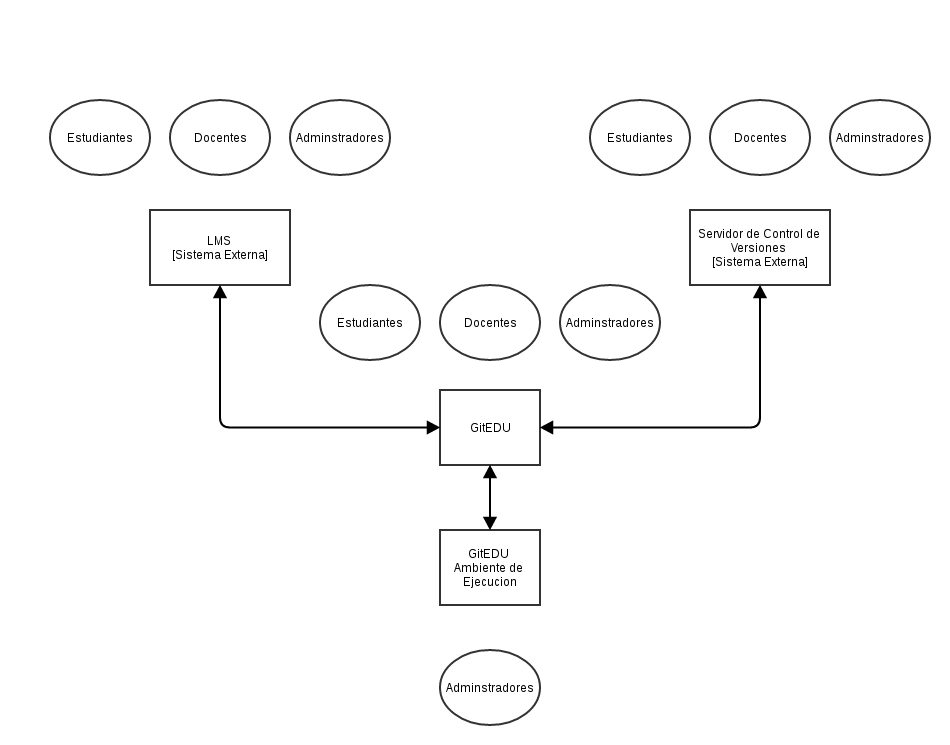
\includegraphics[width=0.75\textwidth]{Figures/pers-prod.png}
  \end{center}
  \caption{Perspectiva del Producto.}
  \label{pers-prod}
\end{figure}

%\pagebreak

\subsection{Resumen de Capacidades}
\begin{table}[h!]
  \begin{tabular}{|p{0.45\textwidth}|p{0.45\textwidth}|}
    \hline
    \textbf{Beneficio al Cliente} & \textbf{Característica de Apoyo} \\
    \hline
    Facilidad de autenticación & Autenticación por LTI contra LMS institucional \\
    \hline
    Gestión de la configuración para el código escrito & Uso de servidores externos de control de versiones \\
    \hline
    Ejecución y pruebas uunitarias en línea & sistema de apoyo con ambiente de ejecución de código \\
    \hline
    Generación y sincronización de notas & calificación a través de pruebas unitarias, sincronización de notas a través de LTI con LMS institucional \\
    \hline
  \end{tabular}
  \caption{Resumen de Capacidades.}
  \label{res-cap}
\end{table}

\subsection{Presuposiciones y Dependencias}
\begin{enumerate}
	\item La institución seguirá usando Moodle y Open EDX como sus plataformas y proveedores de LMS.
	\item La institución seguirá usando como proveedor de un servidor de control de versiones de la institución, un servidor institucional con GitLab Community Edition.
	\item Alternativas como Repl.it y Cloud9 IDE no dan la funcionalidad necesaria o son demasiados costosos para su uso general por la institución.
\end{enumerate}

%\pagebreak

\section{Caracteristicas de Producto}
\begin{enumerate}
	\item Caracteristicas de Autenticación
    	\begin{enumerate}
			\item Autenticarse por LTI
			\item Autenticarse con Usuario y Contraseña
			\item Cerrar Session   
    	\end{enumerate}
    
	\item Caracteristicas de Editar Código
    	\begin{enumerate}
			\item Nuevo Proyecto
			\item Nuevo Proyecto basado en otro Proyecto
			\item Ver Proyectos
			\item Ver Detalles de un Proyecto
			\item Editar Detalles de un Proyecto
			\item Gestionar Usuarios de un Proyecto
			\item Gestionar Permisos de un Proyecto
			\item Abrir Proyecto
			\item Editar Archivos en un Proyecto
			\item Crear Nuevo Archivo en un Proyecto
			\item Borrar Archivo de un Proyecto
			\item Interactuar con Usuarios dentro de un Proyecto
    	\end{enumerate}
    
	\item Caracteristicas de Persistencia de Codigo
    	\begin{enumerate}
			\item Guardar cambios en un Proyecto
			\item Subir cambios en un Proyecto
			\item Bajar cambios en un Proyecto
    	\end{enumerate}
	\item Caracteristicas de Ejecutar y Calificar Código
    	\begin{enumerate}
			\item Ejecutar Codigo en ambiente interactivo en el navegador
			\item Agregar Pruebas Unitarias a un Proyecto
			\item Ejecutar Pruebas Unitarias en un Proyecto
			\item Calificar un Proyecto
			\item Calificiar un Proyecto de forma Automática en base a Pruebas Unitarias
			\item Enviar Calificaciones a un Sistema Externo
    	\end{enumerate}
\end{enumerate}

\pagebreak

\section{Precedencia y Prioridades}
\begin{table}[h!]
  \begin{tabular}{|p{0.45\textwidth}|p{0.45\textwidth}|}
    \hline
    \textbf{Prioridad} & \textbf{Característica (Según su número)} \\
    \hline
    Alta & 1.a, 1.c, 2.a, 2.b, 2.c, 2.h, 2.i, 3.a, 3.b, 4.a \\
    \hline
    Media & 1.b, 2.f, 2.g, 2.j, 3.c, 4.b, 4.c, 4.d, 4.f \\
    \hline
    Baja & 2.d, 2.e, 2.k, 2.l, 4.e \\
    \hline
  \end{tabular}
  \caption{Precedencia y Prioridades.}
  \label{precedencia-y-prioridades}
\end{table}

\section{Restricciones}
\subsection{Seguridad}
Protección contra ataques en la red

Aislamiento de ambientes de ejecución de código de usuarios
\subsection{Extensibilidad}
Soporte al nivel de sistema y documentación para extensión con más lenguajes de programación y motores de base de datos al futuro
\subsection{Usabilidad}
Ser usable

Requerir un mínimo de interacción del usuario para que puede enfocarse en realizar sus responsabilidades en el sistema
\subsection{Escalabilidad}
Tener capacidad para escalar frente mayor carga en el futuro
\subsection{Rendimiento}
Minimizar las requerimientos mínimos de hardware requerido
\section{Otros Requisitos de Producto}
\subsection{Normas}
Ninguna.
\subsection{Requisitos de Sistema}
Ninguno.
\subsection{Requisitos de Rendimiento}
Ninguno.
\subsection{Requisitos Ambientales}
Ninguno.
\section{Requisitos de Documentación}
\subsection{Manual del Programador}
Documentación para explicar el funcionamiento de la aplicación para que futuros desarrolladores puedan extender sin mayor dificultad la aplicación.
\subsection{Manual de Mantenimiento}
Documentación para definir los procesos de mantenimiento de la aplicación para guiar la gobernanza y administración del mismo.
\subsection{Manual de Usuario}
Documentación para enseñar el uso de la aplicación a docentes y alumnos.



% Appendix B - Software Requirements Specification

\chapter{Especificacion de Requisitos de Software}

% Appendix C-E - Apendices de Desarrollo

%\chapter{Frequently Asked Questions} % Main appendix title

\chapter{Preparaciones de Desarrollo}
\label{AnexoC} % For referencing this appendix elsewhere, use \ref{AppendixA}

\section{Servicios Nativos}
% TODO: Intro to Section?

\subsection{Servidor de Git}
Instalar paquetes para un interfaz web sencilla de Git:
\begin{lstlisting}
apt install git gitweb fcgiwrap
\end{lstlisting}

Se crea un usuario del sistema operativo solo para Git:
\begin{lstlisting}
adduser git
\end{lstlisting}

Se autentica como el usuario creado:
\begin{lstlisting}
su - git
\end{lstlisting}

Para tener repositorios ejemplares, se clona algunos repositorios:
\begin{lstlisting}
git clone --bare\
	https://gitlab.com/nishedcob/GitEDU.git\
	repositories/GitEDU.git
git clone --bare\
	https://gitlab.com/ArqAppGrpBravoEarleyVargas/\
    	GitEduERP.git\
	repositories/GitEduERP.git
\end{lstlisting}

Entrar al directorio de repositorios y arreglar permisos para permitir git push desde repositorios remotos:
\begin{lstlisting}
cd repositories/
for repo in `ls`; do
	cd $repo;
    pwd;
    chmod -R g+ws .;
    chgrp -R git .;
    git --bare update-server-info;
    cp hooks/post-update.sample hooks/post-update;
    chmod a+x hooks/post-update;
    cd ..;
done
\end{lstlisting}

Después se configura NGinX para trabajar con gitweb:
\begin{lstlisting}
# NGinX Config:
server {
        listen 80;
        listen [::]:80;
        server_name git.localhost 192.168.99.1 10.10.10.1;
        root /usr/share/gitweb;
        access_log /var/log/nginx/gitweb.access.log;
        # static repo files for cloning over https
        location ~ ^.*\.git/objects/([0-9a-f]+/[0-9a-f]+\
        	|pack/pack-[0-9a-f]+.(pack|idx))$ {
                root /home/git/repositories/;
        }

        # requests that need to go to git-http-backend
        location ~ ^.*\.git/(HEAD|info/refs|objects/info/.*\
        	|git-(upload|receive)-pack)$ {
                root /home/git/repositories;

                fastcgi_pass unix:/var/run/fcgiwrap.socket;
                fastcgi_param SCRIPT_FILENAME   /usr/lib/\
                	git-core/git-http-backend;
                fastcgi_param PATH_INFO          $uri;
                fastcgi_param GIT_PROJECT_ROOT  /home/git/\
                	repositories;
                fastcgi_param GIT_HTTP_EXPORT_ALL "";
                fastcgi_param REMOTE_USER $remote_user;
                include fastcgi_params;
        }

        # send anything else to gitweb if it's not a real file
        try_files $uri @gitweb;
        location @gitweb {
                fastcgi_pass unix:/var/run/fcgiwrap.socket;
                fastcgi_param SCRIPT_FILENAME   /usr/share/\
                	gitweb/gitweb.cgi;
                fastcgi_param PATH_INFO          $uri;
                fastcgi_param GITWEB_CONFIG      /etc/gitweb\
                	.conf;
                include fastcgi_params;
        }
}
\end{lstlisting}

Además se configura gitweb con la siguiente configuración:
\begin{lstlisting}
# Edit /etc/gitweb.conf
# path to git projects (<project>.git)
#$projectroot = "/var/lib/git";
$projectroot = "/home/git/repositories";
\end{lstlisting}

Prueba de que funciona:
\begin{lstlisting}
git clone http://git.localhost/nishedcob/GitEDU.git \
	GitEDU-test
\end{lstlisting}

Dado que el mismo GitWeb no tenga problemas con bajada de datos (\texttt{git fetch} / \texttt{git pull} / \texttt{git clone}) pero si tiene problemas con subida de datos como se lo require en EduNube para armar repositorios de ejecuccion validadas, se ve una necesidad de habilitar subida al mismo por SSH:

Como root en el servidor de Git, se cambia la clave del usuario de Git:
\begin{lstlisting}
passwd git
\end{lstlisting}

Como el usuario de EduNube en el servidor para el mismo:
\begin{lstlisting}
cd .ssh/
# Deja la llave generada sin clave:
ssh-keygen -f id_git
# Copia la llave publica al servidor
ssh-copy-id -i ~/.ssh/id_git.pub git@10.10.10.1
# Prueba que funciona
ssh -i ~/.ssh/id_git -vvv git@10.10.10.1
# Guardar la configuracion:
cat >> ~/.ssh/config < EOF

Host git
     HostName 10.10.10.1
     User git
     Port 22
     IdentityFile $HOME/.ssh/id_git

EOF
# Probar con:
ssh -vvv git
\end{lstlisting}

\section{Servicios Virtualizados}
% TODO: Section Introduction?

\subsection{Maquina Virtual de Xen para Moodle}
Para el ambiente de Moodle (LMS \index{LMS} contra el cual se ha llevado el desarrollo), se crea una maquina virtual de Debian Stretch (9) con 1 GiB de RAM, 1 CPU virtual, 6 GiB de disco, 512 MiB de intercambio y una dirección IP fija de 10.10.10.10. Los resultados del mismo comando se puede ver en la figura \ref{vm-moodle}.
\begin{lstlisting}
	xen-create-image --hostname=debian-moodle\
    		--ip=10.10.10.10 --netmask=255.255.255.0\
        	--gateway=10.10.10.1 --memory=1024mb\
        	--vcpus=1 --lvm=Xephyr-VG --pygrub\
        	--dist=stretch --force --size=6144mb\
        	--swap=512mb
\end{lstlisting}

\begin{figure}
	\begin{center}
    	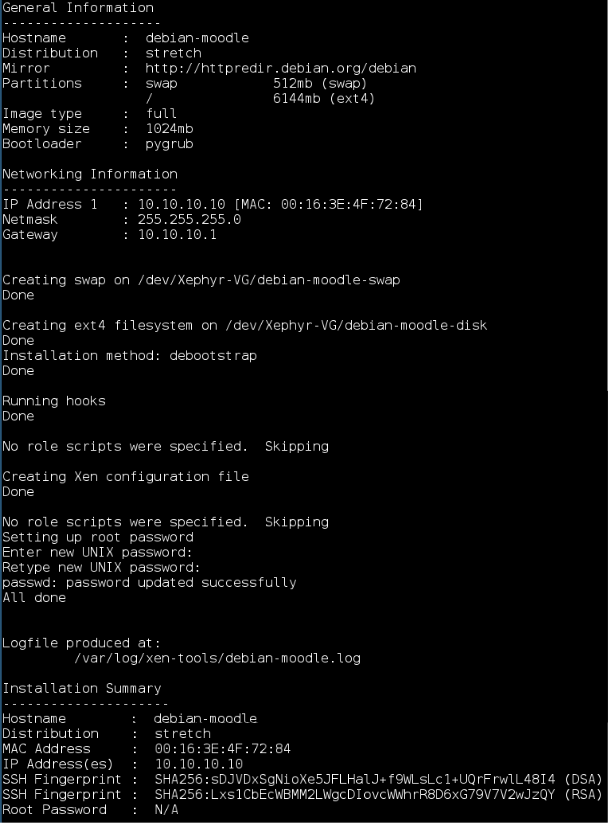
\includegraphics[width=0.75\textwidth]{Figures/crear-moodle.png}
    \end{center}
  	\caption{Crear maquina virtual para Moodle.}
    \label{vm-moodle}
\end{figure}

Se renombró el archivo de configuración de la maquina virtual generado en el paso anterior para temas de consistencia.

\begin{lstlisting}
	mv /etc/xen/debian-moodle.cfg\
    		/etc/xen/domU-debian-moodle.cfg
\end{lstlisting}

Un bug de Xen-Tools causa que no se instala correctamente un núcleo de Linux en la maquina virtual y por lo tanto es necesario entrar al mismo con un Chroot y instalar los paquetes faltantes (y hacer las adecuadas configuraciones para permitir su arranque independiente de ayuda externa)\footnote{6 meses despues de la redaccion de estos pasos, y Xen-Tools ya no tiene este bug, motivo por el cual se puede emitir este paso si es que la maquina virtual esta funcionando de forma correcta.}.

\begin{lstlisting}
	mount /dev/Xephyr-VG/debian-moodle-disk /mnt
	mount -o bind /proc /mnt/proc
	mount -o bind /sys /mnt/sys
	mount -o bind /dev /mnt/dev
	cp /etc/resolv.conf /mnt/etc/resolv.conf
	chroot /mnt /bin/bash
	apt install linux-image-amd64
	vim.tiny /boot/grub/menu.lst
	# Revisar que los archivos referenciados existen
	#		de verdad por ejemplo:
	# Replace initrd.img- con initrd.img
    # guarda y sale
	exit
	umount /mnt/proc            
	umount /mnt/sys 
	umount /mnt/dev 
	umount /mnt	
\end{lstlisting}

Para levantar la maquina virtual:

\begin{lstlisting}
	xl create /etc/xen/domU-debian-moodle.cfg -c
\end{lstlisting}

Se debe seleccionar la tercera opción (Default Kernel).

Se puede dar una revisión a la configuración de red para asegurarse de que esta correcto:

\begin{lstlisting}
	vim.tiny /etc/network/interfaces
\end{lstlisting}

Debe contener:

\begin{lstlisting}
auto eth0
iface eth0 inet static
 address 10.10.10.10
 gateway 10.10.10.1
 netmask 255.255.255.0
\end{lstlisting}

En el presente caso, Xen-Tools logró configurar esta parte de forma correcta.

A continuación se procede con la instalación de Moodle:

\begin{lstlisting}
# actualiza el sistema
apt update
apt upgrade

# instala dependencias
apt install apache2 php7.0 mysql-server php7.0-mysql
apt install libapache2-mod-php7.0 php7.0-gd php7.0-curl
apt install php-xml php-zip php-mbstring php-soap
apt install php7.0-xmlrpc php7.0-intl
vim.tiny /etc/php/7.0/apache2/php.ini

# agrega:
extension=mysql.so 
extension=gd.so

# edita:

memory_limit = 40M
# dejado con el valor por defecto de 128M

post_max_size = 80M
upload_max_filesize = 80M

# guarda y sale

# reinicia apache para coger los cambios
systemctl restart apache2

\end{lstlisting}

A continuación se configura la base de datos:

\begin{lstlisting}

# clave de root es root
mysqladmin -u root password "root"

# iniciar session como root
mysql -u root -p

# crear base de datos y hacer que ocupa UTF-8
mysql> CREATE DATABASE moodle;
mysql> ALTER DATABASE moodle charset=utf8;
mysql> exit;

## No se implemento ##
# Moodle queja de UTF8

# Se podria arreglar
# (antes de instalar Moodle)
# con:

mysql -u root -p

mysql> ALTER DATABASE moodle charset=utf8mb4;
mysql> exit;
######################

systemctl restart mysql

\end{lstlisting}

Se realiza la instalación de la ultima versión de Moodle (3.3 con sus respectivos patches de fallas desde que el mismo salio):

\begin{lstlisting}

# descargar
wget https://download.moodle.org/download.php/direct/stable33/\
	moodle-latest-33.tgz

# descomprimir
tar -zxvf moodle-latest-33.tgz

# meter en la ubicacion para apache
mv moodle /var/www

# ir a ubicacion para apache
cd /var/www

# crear ubicacion para datos
mkdir moodledata

# arreglar permisos
chown -R www-data:www-data moodle
chown -R www-data:www-data moodledata
chmod -R 755 moodle
chmod -R 755 moodledata

# modificar configuracion de apache
vim.tiny /etc/apache2/sites-available/000-default.conf

# editar
DocumentRoot "/var/www/moodle"

# guardar y salir

# reiniciar apache para aplicar los cambios
systemctl restart apache2

\end{lstlisting}

Arreglar la base de datos para que acepte conexiones desde Moodle:

\begin{lstlisting}

mysql -u root -p

GRANT ALL PRIVILEGES on *.* to
	'root'@'localhost' IDENTIFIED BY 'root';
GRANT ALL PRIVILEGES on *.* to
	'root'@'localhost' IDENTIFIED BY 'root';
FLUSH PRIVILEGES;
exit;

\end{lstlisting}

Para seguir con la instalación se abre un navegador con la dirección \url{http://10.10.10.10/} para seguir las instrucciones que se le lleve por toda la configuración inicial del Moodle.

Al final se agregue un trabajo de cron para ayudar con los tareas periódicas que Moodle requiere para su mantenimiento continuo:

\begin{lstlisting}

crontab -u www-data -e
# add line:
*/10 * * * * /usr/bin/php
		/var/www/moodle/admin/cli/cron.php
        		>/dev/null

\end{lstlisting}

Estos pasos fueron adaptados de la guía oficial del proyecto de Moodle para instalación en Debian \citep{MOODLE-Install-Debian}.

Ahora que todo esta funcionando se recomienda editar /boot/grub/menu.lst para comentar las entradas del pyGrub que son defectuosas (los primeros dos) para que se puede levantar la maquina virtual sin intervención humana.

\subsection{Máquina Virtual de Xen}
Para crear el servidor de Git con GitLab Community Edition, se va a empezar con las mismas piezas del servidor del LMS/Moodle, es decir una maquina virtual de Debian 9. El mismo se crea como una maquina virtual de Debian Stretch (9) con 1 GiB de RAM, 1 CPU virtual, 6 GiB de disco, 512 MiB de intercambio y una dirección IP fija de 10.10.10.11.
\begin{lstlisting}
	xen-create-image --hostname=debian-gitlab\
    		--ip=10.10.10.11 --netmask=255.255.255.0\
        	--gateway=10.10.10.1 --memory=1024mb\
        	--vcpus=1 --lvm=Xephyr-VG --pygrub\
        	--dist=stretch --force --size=6144mb\
        	--swap=512mb
\end{lstlisting}

Se renombró el archivo de configuración de la maquina virtual generado en el paso anterior para temas de consistencia.

\begin{lstlisting}
	mv /etc/xen/debian-gitlab.cfg\
    		/etc/xen/domU-debian-gitlab.cfg
\end{lstlisting}

Un bug de Xen-Tools causa que no se instala correctamente un núcleo de Linux en la maquina virtual y por lo tanto es necesario entrar al mismo con un Chroot y instalar los paquetes faltantes (y hacer las adecuadas configuraciones  para permitir su arranque independiente de ayuda externa)\footnote{6 meses despues de la redaccion de estos pasos, y Xen-Tools ya no tiene este bug, motivo por el cual se puede emitir este paso si es que la maquina virtual esta funcionando de forma correcta.}.

\begin{lstlisting}
	mount /dev/Xephyr-VG/debian-gitlab-disk /mnt
	mount -o bind /proc /mnt/proc
	mount -o bind /sys /mnt/sys
	mount -o bind /dev /mnt/dev
	cp /etc/resolv.conf /mnt/etc/resolv.conf
	chroot /mnt /bin/bash
	apt install linux-image-amd64
	vim.tiny /boot/grub/menu.lst
	# Revisar que los archivos referenciados existen
	#		de verdad por ejemplo:
	# Replace initrd.img- con initrd.img
    # guarda y sale
	exit
	umount /mnt/proc            
	umount /mnt/sys 
	umount /mnt/dev 
	umount /mnt	
\end{lstlisting}

Para levantar la maquina virtual:

\begin{lstlisting}
	xl create /etc/xen/domU-debian-gitlab.cfg -c
\end{lstlisting}

Se debe seleccionar la tercera opción (Default Kernel).

Se puede dar una revisión a la configuración de red para asegurarse de que esta correcto:

\begin{lstlisting}
	vim.tiny /etc/network/interfaces
\end{lstlisting}

Debe contener:

\begin{lstlisting}
auto eth0
iface eth0 inet static
 address 10.10.10.11
 gateway 10.10.10.1
 netmask 255.255.255.0
\end{lstlisting}

En el presente caso, Xen-Tools logró configurar esta parte de forma correcta.

A continuación se procede con la instalación de Gitlab:

\begin{lstlisting}
# actualiza el sistema
apt update
apt upgrade

# A partir del Debian 9, Gitlab CE esta ofrecido
#    en los repositorios oficiales:
apt install gitlab

# Arreglar problema con API
vim.tiny /usr/share/gitlab-shell/config.yml
# cambiar gitlab_url a "http://10.10.10.11/"

/usr/share/gitlab-shell/bin/check
\end{lstlisting}

Visitar \url{http://10.10.10.11/} y configurar la contraseña del usuario root. Con el usuario root configurado se procede a crear un usuario especial para la aplicación con el nombre de usuario 'GitEdu'. Este usuario lo damos permisos de administración y también se genera un token en esta dirección: \url{http://10.10.10.11/profile/personal_access_tokens}. El token se debe guardar para su uso después (GitLab nunca le vuelve a mostrar).

Ahora que todo esta funcionando se recomienda editar /boot/grub/menu.lst para comentar las entradas del pyGrub que son defectuosas (los primeros dos) para que se puede levantar la maquina virtual sin intervención humana.

\section{Kubernetes}
% TODO: Introduccion a Kubernetes?

\index{Kubernetes}
\subsection{Instalación de Kubernetes}
Para instalar la ultima version del cliente de Kubernetes, tanto en desarrollo como en produccion, solo se necesita bajar la ultima version de kubectl desde los repositorios de Google y poner el mismo dentro del \$PATH:
\begin{lstlisting}[breaklines=true]
# Bajar la ultima version de Kubectl para Linux:
curl -LO https://storage.googleapis.com/kubernetes-release/\
	release/$(curl -s https://storage.googleapis.com/\
    	kubernetes-release/release/stable.txt)\
	/bin/linux/amd64/kubectl
# Hacerlo ejecutable
chmod +x kubectl
# Revisar el $PATH actual
echo $PATH
# Ubicar dentro del $PATH
mv kubectl ~/bin/
# verificar instalacion con:
kubectl --help
# o con:
kubectl version
# Este segundo commando debe dar un error de servidor hasta\
#	que se instala y configura el servidor al cual se\
#	debe connectar
\end{lstlisting}

\index{Kubernetes}
\subsection{MiniKube}
Dentro del ambiente de desarrollo, fue ocupado un cluster de Kubernetes, de solo un nodo, virtualizado en VirtualBox. La instalacion del mismo se detalle a continuacion:
\begin{lstlisting}[breaklines=true]
# Se descarga desde los repositorios de Google el commando de MiniKube
curl -Lo minikube https://storage.googleapis.com/minikube/releases/v0.23.0/minikube-linux-amd64
# Se lo hace ejecutable
chmod +x minikube
# se lo ubica en el $PATH
mv minikube ~/bin/
# para validar la instalacion:
minikube --help
# o
minikube version
\end{lstlisting}

Para levantar el cluster de MiniKube y realizar la configuracion automatica del entorno para el uso del mismo, se utiliza el commando:
\begin{lstlisting}
minikube start
\end{lstlisting}

Para bajar el cluster de MiniKube:
\begin{lstlisting}
minikube stop
\end{lstlisting}
\index{Contenedor} \index{Virtualización} \index{Hipervisor}

\index{Docker|(}
\section{Docker}
% TODO: Introduccion?

\subsection{Tipo de Contenedor: Shell-Executor}
% TODO: Introduccion?

\subsubsection{Debian}
El Debian Shell-Executor se crea con los siguientes lineas en el Dockerfile: 
\begin{lstlisting}[breaklines=true]
FROM debian:stretch

ENV shell=/bin/sh
ENV user=user

# Greatly increases image size, optional:
#RUN apt-get update && apt-get install -y lsb-release

RUN mkdir -p /code && echo "USER=$user" && echo "SHELL=$shell" && useradd -ms $shell $user && chown -v $user:$user /code
VOLUME ["/code"]

ENTRYPOINT ["/bin/sh"]
CMD ["/code/exec.sh"]
\end{lstlisting}
La primera linea, ''FROM ...'' define el imagen base, en este caso la versión actual de Debian Stretch (Debian 9.x). La tercera y cuarta linea, ''ENV ...'', definen variables de entorno que se puede cambiar previa a la construcción del imagen en adición a sus valores por defecto. La sexta y séptima linea, documenta y define un paso opcional donde se instala un paquete adicional, lsb-release, que provee información estandarizado de la distribución de Linux en ejecución. Este paso opcional agrega mucho peso al contenedor y por lo tanto no se lo ha dejado comentado. La novena y décima linea define comandos preliminares para preparar el contenedor como:
\begin{itemize}
	\item Crear una carpeta "/code" donde se puede copiar el código a ser ejecutado desde afuera del contenedor
	\item Visualización los variables de entorno para temas informativos y de debug
	\item La creación del usuario que vamos a utilizar dentro del contenedor
	\item Dar el usuario los permisos adecuados para que tiene acceso a la carpeta creada
\end{itemize}
La onceava linea define la carpeta creada como un volumen de Docker, el cual se monta externamente al crear y ejecutar el contenedor. La decimotercera linea define el argumento cero del contenedor al momento de iniciar la misma, en este caso el shell que se encuentra del contenedor. La decimocuarta linea define los argumentos con que se debe ejecutar el comando definido previamente, en este caso el script de entrada, cargado desde un sistema de ficheros externo al contenedor.

\subsubsection{Alpine Linux}
El Alpine Shell-Executor se crea con los siguientes lineas en el Dockerfile: 
\begin{lstlisting}
FROM alpine:3.6

ENV shell=/bin/sh
ENV user=user

RUN mkdir -p /code && echo "USER=$user" && echo "SHELL=$shell"\
&& echo "SHELL is not used in this Dockerfile" &&\
    adduser -D $user && chown -v $user:$user /code
VOLUME ["/code"]

ENTRYPOINT ["/bin/sh"]
CMD ["/code/exec.sh"]
\end{lstlisting}
La primera linea, ''FROM ...'' define el imagen base, en este caso la versión actual de Alpine Linux (Alpine 3.6). La tercera y cuarta linea, ''ENV ...'', definen variables de entorno que se puede cambiar previa a la construcción del imagen en adición a sus valores por defecto. La sexta, séptima y octava lineas define comandos preliminares para preparar el contenedor como:
\begin{itemize}
	\item Crear una carpeta "/code" donde se puede copiar el código a ser ejecutado desde afuera del contenedor
	\item Visualización los variables de entorno para temas informativos y de debug
	\item La creación del usuario que vamos a utilizar dentro del contenedor
	\item Dar el usuario los permisos adecuados para que tiene acceso a la carpeta creada
\end{itemize}
La novena linea define la carpeta creada como un volumen de Docker, el cual se monta externamente al crear y ejecutar el contenedor. La onceava linea define el argumento cero del contenedor al momento de iniciar la misma, en este caso el shell que se encuentra del contenedor. La duodécima linea define los argumentos con que se debe ejecutar el comando definido previamente, en este caso el script de entrada, cargado desde un sistema de ficheros externo al contenedor. 

\subsection{Tipo de Contenedor: Python3-Executor}
% TODO: Introduction?

\subsubsection{Debian}
El Debian Python3-Executor se define de la siguiente manera a través de su Dockerfile:
\begin{lstlisting}[breaklines=true]
FROM registry.gitlab.com/nishedcob/gitedu/shell-executor:debian-stretch

RUN apt-get update && apt-get install -y python3 python3-dev python3-pip virtualenv

VOLUME ["/code"]
WORKDIR "/code"
\end{lstlisting}
La primera y segunda linea define herencia del contenedor Debian Shell-Executor que definimos previamente. La tercera y cuarta linea instala Python3, Pip3 y Virtualenv dentro del contenedor. La sexta linea vuelve a declarar el volumen de Docker porque al aparecer la versión actual de Docker a propósito no suporta herencia de esta linea en los Dockerfile. La séptima linea define la ubicación inicial utilizada cuando se inicia el contenedor.

\subsubsection{Alpine Linux}
El Alpine Python3-Executor se define a través del Dockerfile que esta a continuación:
\begin{lstlisting}[breaklines=true]
FROM registry.gitlab.com/nishedcob/gitedu/shell-executor:alpine-3.6

RUN apk update && apk add python3 python3-dev py-virtualenv

VOLUME ["/code"]
WORKDIR "/code"
\end{lstlisting}
La primera y segunda linea define herencia del contenedor Alpine Shell-Executor que definimos previamente. La tercera linea instala Python3, Pip3 y Virtualenv dentro del contenedor. La quinta linea vuelve a declarar el volumen de Docker porque al aparecer la versión actual de Docker a propósito no suporta herencia de esta linea en los Dockerfile. La sexta linea define la ubicación inicial utilizada cuando se inicia el contenedor.

\subsection{Tipo de Contenedor: PostgreSQL-Executor}
% TODO: introduccion?

\subsubsection{Debian}
El Debian PostgreSQL-Executor se define con el siguiente Dockerfile:
\begin{lstlisting}[breaklines=true]
FROM registry.gitlab.com/nishedcob/gitedu/shell-executor:debian-stretch

RUN apt-get update && apt-get install -y postgresql postgresql-client

RUN echo "Starting PostgreSQL Cluster..." ; /usr/bin/pg_ctlcluster 9.6 main start && echo "Started cluster!" || echo "Failed to start cluster!"; su - postgres -c "createuser user && createdb -O user userdb"; echo "Stopping PostgreSQL Cluster..." ; /usr/bin/pg_ctlcluster 9.6 main stop && echo "Stopped cluster!" || echo "Failed to stop cluster!";

VOLUME ["/code"]
WORKDIR "/code"
\end{lstlisting}
La primera y segunda linea define herencia del contenedor Debian Shell-Executor que definimos previamente. La tercera y cuarta linea instala PostgreSQL dentro del contenedor. La sexta hasta décima linea levanta el motor de base de datos PostgreSQL con la finalidad de crear un usuario y base de datos por defecto sobre el cual se puede trabajar. Finalizando este proceso se desactiva el contenedor para reducir el tamaño del mismo y no introducir comportamiento desconocido. La duodécima linea vuelve a declarar el volumen de Docker porque al aparecer la versión actual de Docker a propósito no suporta herencia de esta linea en los Dockerfile. La decimotercera linea define la ubicación inicial utilizada cuando se inicia el contenedor.

\subsubsection{Alpine Linux}
El Alpine PostgreSQL-Executor se define con el siguiente Dockerfile:
\begin{lstlisting}[breaklines=true]
FROM registry.gitlab.com/nishedcob/gitedu/shell-executor:alpine-3.6

RUN apk update && apk add postgresql && su - postgres -c "export PGDATA=/var/lib/postgresql/data && initdb"

RUN echo "Starting PostgreSQL Cluster..." ; mkdir -p /run/postgresql && chown -R postgres:postgres /run/postgresql && chmod 755 /run/postgresql && mkdir -p /var/run/postgresql && chown -R postgres:postgres /var/run/postgresql && chmod 2777 /var/run/postgresql && su - postgres -c "export PGDATA=/var/lib/postgresql/data && postgres &" && echo "Started cluster!" || echo "Failed to start cluster!"; sleep 5s && netstat -tupln && su - postgres -c "createuser user && createdb -O user userdb"; echo "Stopping PostgreSQL Cluster..." ; killall postgres && echo "Stopped cluster!" || echo "Failed to stop cluster!";

VOLUME ["/code"]
WORKDIR "/code"
\end{lstlisting}
La primera y segunda linea define herencia del contenedor Alpine Shell-Executor que definimos previamente. La tercera y cuarta linea instala PostgreSQL dentro del contenedor en adición a inicializar la base de datos. La sexta hasta decimoséptima linea levanta el motor de base de datos PostgreSQL con la finalidad de crear un usuario y base de datos por defecto sobre el cual se puede trabajar. Finalizando este proceso se desactiva el contenedor para reducir el tamaño del mismo y no introducir comportamiento desconocido. La decimonovena linea vuelve a declarar el volumen de Docker porque al aparecer la versión actual de Docker a propósito no suporta herencia de esta linea en los Dockerfile. La vigésima linea define la ubicación inicial utilizada cuando se inicia el contenedor.
\index{Docker|)}

\chapter{Desarollo de GitEDU}
\label{AnexoD}

\section{Configuracion de la Base de Datos Relacional}
Primero es necesario crear y configurar un usuario y base de datos para ser ocupado:
\begin{lstlisting}
postgresql-setup initdb
systemctl enable postgresql
systemctl start postgresql
systemctl status postgresql
vim /etc/postgresql/9.6/main/pg_hba.conf
# agregar una linea antes de las lineas similares y
# que diga (sin el numeral adelante):
#local   all      postgres             peer
systemctl restart postgresql
systemctl status postgresql
su - postgres
psql
\end{lstlisting}
\begin{lstlisting}
	postgres=# CREATE USER giteduser WITH PASSWORD 'g1T3d_$3r';
	postgres=# CREATE DATABASE gitedudb WITH OWNER giteduser;
	postgres=# \q
psql gitedudb -U postgres
	gitedudb=# CREATE SCHEMA giteduapp AUTHORIZATION giteduser;
	gitedudb=# ALTER USER giteduser SET search_path TO giteduapp;
	gitedudb=# \q
psql gitedudb -U giteduser
	gitedudb=> SELECT current_schema();
		Debe decir: giteduapp
	gitedudb=> \q
\end{lstlisting}

Segundo, se abre el settings.py (dentro de la carpeta GitEDU/GitEDU) y se remplaza (para desarrollo, en producción debe llevar valores distintos) el atributo DATABASES con lo siguiente:
\lstset{language=Python}
\begin{lstlisting}
DATABASES = {
    'default': {
        'ENGINE': 'django.db.backends.postgresql_psycopg2',
        'NAME': 'gitedudb',
        'USER': 'giteduser',
        'PASSWORD': 'g1T3d_$3r',
        'HOST': '127.0.0.1',
        'PORT': '5432',
    }
}
\end{lstlisting}
\lstset{language=Bash}

\section{Configuracion de la Base de Datos No Relacional}
Para crear la base de datos de MongoDB:
\begin{lstlisting}
mongo
\end{lstlisting}
\lstset{language=sql}
\begin{lstlisting}
use gitEduDB
db.createUser(
    {
        user: "gitEduUser",
        pwd: "G1TedU$3r",
        roles: [ "readWrite", "dbAdmin" ]
    }
)
\end{lstlisting}
\lstset{language=Bash}

El mismo se define en el settings de la siguiente manera:
\lstset{language=Python}
\begin{lstlisting}
NOSQL_DATABASES = {
    'nosql': {
        'NAME': 'gitEduDB',
        'USER': "gitEduUser",
        'PASSWORD': 'G1TedU$3r',
        'HOST': '127.0.0.1',
        'PORT': '27017',
    }
}
\end{lstlisting}
\lstset{language=Bash}

\section{Compatibilidad con EduNube en el Mismo Repositorio}
Para reducir el numero de repositorios involucrados en este trabajo de titulación, se ha optado por llevar el desarrollo de EduNube dentro del mismo repositorio, con una separación de dependencias con otro entorno virtual y aislamiento de código en desarrollo con varias ramas de Git. Por lo tanto, se realizo una nueva rama de Git con el comando:
\begin{lstlisting}
git checkout -b gitedu
\end{lstlisting}

Y una refacturación del entorno virtual a ser ''env-ge'' en lugar de ''env'', en lugar de ''requirements.txt'', utilizar ''requirements.ge.txt'' y un nuevo script de activar el entorno, el cual se activa ahora con ''source activate-ge.sh'':
\begin{lstlisting}
#! /usr/bin/head -n 2 
# run with `source activate-ge.sh`
PROJECT=ge
ENV_DIR=env-$PROJECT
if [ ! -d $ENV_DIR ]; then
	virtualenv --python=python3 $ENV_DIR
fi
source $ENV_DIR/bin/activate
pip3 install -r requirements.$PROJECT.txt
\end{lstlisting}

Para desarrollar ambos sistemas en paralelo, y poder trabajar en ramas independientes con ambos sistemas levantados al mismo tiempo para probar y desarrollar características de integración, se clono de forma local el repositorio:
\begin{lstlisting}
git clone GitEDU GitEDU-copy
\end{lstlisting}

Para el desarrollo se ocupa el puerto 8000 de localhost para GitEDU y el puerto 8001 de localhost para EduNube:
\begin{lstlisting}
# Levantar GitEDU en el ambiente de desarrollo:
cd GitEDU-copy
source activate-ge.sh
git checkout gitedu
cd GitEDU
python manage.py runserver 8000

# Levantar EduNube en el ambiente de desarrollo:
cd GitEDU
source activate-en.sh
git checkout edunube
cd EduNube
python manage.py runserver 8001
\end{lstlisting}\footnote{Para produccion, se cambio el puerto 8001 de EduNube para 8010}


\index{Autenticación LTI}
\section{Autenticacion por LTI}
Primero es necesario que este activo y levantado el ambiente del LMS \index{LMS} como se documenta en la sección \ref{instalacion-moodle} de instalación de Moodle. Para el desarrollo de este trabajo de titulación se esta considerando una instalación en un servidor aparte (virtualizado en el mismo equipo) en la dirección IP 10.10.10.10.

% Instalar dependencias

Instalación de dependencias desde GitHub (no se encuentran en los repositorios oficiales de Pip/Pypi; además para superar problemas de dependencias en las librerías, se ha optado para ocupar forks personales del autor con las mejores necesarias para su funcionamiento):
\begin{lstlisting}
pip install git+https://github.com/nishedcob/django-app-lti
    @master#egg=django-app-lti
pip install git+https://github.com/nishedcob/
    django-auth-lti@master#egg=django-auth-lti
\end{lstlisting}

Como son dependencias no se encuentran en los repositorios oficiales, su manejo dentro del requirements.txt también tiene que ser especial ya que un `pip freeze` no los guardaran correctamente dentro del mismo. En lugar de eso hay que agregar dos lineas al requirements.txt para el manejo de estas dependencias:
\begin{lstlisting}
-e git+https://github.com/nishedcob/django-app-lti.git
    @38b32989e22b189345e421b183684f9b5453e99a
    #egg=django-app-lti
-e git+https://github.com/nishedcob/django-auth-lti.git
    @71c9da8d0aa07ebc3139bf3f113b5c521d61b1f1
    #egg=django-auth-lti
\end{lstlisting}

% Modificar settings

\lstset{language=Python}

Se pone a editar el settings.py (dentro de GitEDU/GitEDU) con las siguientes configuraciones:
\begin{itemize}
	\item a INSTALLED\_APPS agregamos las siguientes lineas:
   		\begin{lstlisting}
    'django_auth_lti',
    'django_app_lti',
    	\end{lstlisting}
    \item a MIDDLEWARE agregamos la siguiente linea:
   		\begin{lstlisting}
    'django_auth_lti.middleware.LTIAuthMiddleware',
    	\end{lstlisting}
    \item a AUTHENTICATION\_BACKENDS agregamos la siguiente linea:
   		\begin{lstlisting}
    'django_auth_lti.backends.LTIAuthBackend',
    	\end{lstlisting}
        Si es que no existe AUTHENTICATION\_BACKENDS lo creamos con los siguientes valores:
        \begin{lstlisting}
AUTHENTICATION_BACKENDS = (
    'django.contrib.auth.backends.ModelBackend',
    'django_auth_lti.backends.LTIAuthBackend',
)
        \end{lstlisting}
    \item también agregamos los siguientes atributos:
    	\begin{itemize}
    		\item LTI\_SETUP
            	\begin{lstlisting}
LTI_SETUP = {
    "TOOL_TITLE": "GitEDU",
    "TOOL_DESCRIPTION": "Sistema para Programar en Linea",
    "LAUNCH_URL": "lti:launch",
    "LAUNCH_REDIRECT_URL": "ideApp:decode",
    "INITIALIZE_MODELS": False,
    "EXTENSION_PARAMETERS": {
        "10.10.10.10": {
            "privacy_level": "public",
            "course_navigation": {
                "enabled": "true",
                "default": "disabled",
                "text": "GitEDU LMS Playground",
            }
        }
    }
}
            	\end{lstlisting}
            \item LTI\_OAUTH\_CREDENTIALS con texto aleatorio (fue ocupado OpenSSL, específicamente el comando \texttt{openssl rand -hex 10} para generar los valores de abajo\footnote{Un ambiente de producción debe ocupar valores distintos}).
            	\begin{lstlisting}
LTI_OAUTH_CREDENTIALS = {
    "GitEduLMS_Playground": "b2e0158c3cb4ddb0202d", 
         # (Para pruebas)
    "GitEduLMS_Playground_Assignments":
         "57b3a14734566c49bcaf",
         # (Para deberes/examenes/pruebas/talleres/etc)
    "GitEduLMS_Playground_Classes":
         "f7a0b6accc2631779e84",
         # (Para materias)
}
            	\end{lstlisting}
    	\end{itemize}
\end{itemize}

También se edita el urls.py (dentro de la misma dirección que el settings.py) con las siguientes lineas:
\begin{lstlisting}
from django.conf.urls import include
import django_app_lti.urls

# dentro de:
urlpatterns = [
    # agregar:
    url(r'^lti/', include(django_app_lti.urls, namespace="lti")),
]

\end{lstlisting}

\lstset{language=Bash}

Para arreglar un problema de una versión muy desactualizada de ims-lti-py, se agrego la siguiente linea al requirements.txt (para ocupar un fork del propio librería por el propio autor para resolver los problemas dados):
\begin{lstlisting}
-e git+https://github.com/nishedcob/ims_lti_py.git
    @a6576d7892ea4f69b76572788b118aaa4cdcf749
    #egg=ims_lti_py-develop
\end{lstlisting}

Para arreglar un problema de limpieza de datos en oauth2, se agrego la siguiente linea al requirements.txt (para ocupar un fork del propio librería por el propio autor para resolver los problemas dados):
\begin{lstlisting}
-e git+https://github.com/nishedcob/python-oauth2.git
    @176fc35aa35d626afcb6a23459482a4c96782c88
    #egg=oauth2
\end{lstlisting}

Después se migra la base de datos:
\begin{lstlisting}
python manage.py makemigrations
python manage.py migrate
\end{lstlisting}

\section{Migracion para llenar tabla AuthenticationType}
Con una migración se puede llenar de forma automática el catalogo de AuthenticacionType:
\lstset{language=Python}
\begin{lstlisting}
def fill_auth_types(apps, schema_editor):
    auth_type = models.AuthenticationType
    classic = auth_type(name="Clasica")
    classic.save()
    lti = auth_type(name="LTI")
    lti.save()


class Migration(migrations.Migration):

    dependencies = [
        ('authApp',
           '0002_authenticationtype_userauthentication'),
    ]

    operations = [
        migrations.RunPython(fill_auth_types),
    ]
\end{lstlisting}
\lstset{language=Bash}

\section{Accesibilidad a Datos de Autetnicacion de LTI}
Primero al settings se agrega dos atributos que indiquen cual llave se considera el sistema para compartir materias y otro para compartir deberes/exámenes/pruebas/talleres/etc\ldots{}:
\lstset{language=Python}
\begin{lstlisting}
LTI_ASSIGNMENTS_KEY = 'GitEduLMS_Playground_Assignments'
LTI_CLASSES_KEY = 'GitEduLMS_Playground_Classes'
\end{lstlisting}
\lstset{language=Bash}

Para controlar las partes de la configuración que se presenta a los usuarios finales, agregamos un nuevo campo de configuración al settings:
\lstset{language=Python}
\begin{lstlisting}
LTI_CONFIG_EXPOSE = {
    "LTI_KEYS": True,
    "LTI_ASSIGNMENT_KEY": True,
    "LTI_CLASS_KEY": True,
    "LTI_OTHER_KEYS": False,
    "LTI_SETUP": False,
}
\end{lstlisting}
\lstset{language=Bash}

Para que los profesores (como usuario final de GitEdu) también tengan acceso a estos credenciales para poderlos ocupar, se cree una vista en la ubicación '/auth/lti/credentials' que devuelve un JSON con los datos de LTI:
\lstset{language=Python}
\begin{lstlisting}[breaklines=true]
class LTICredentialsView(View):

    def get(self, request):
        if not request.user.is_authenticated:
            raise PermissionError("No tiene acceso a esta vista hasta que se autentica...")

        lti_expose = settings.LTI_CONFIG_EXPOSE

        lti_cred_json = {}

        if lti_expose['LTI_KEYS']:
            if lti_expose['LTI_ASSIGNMENT_KEY']:
                lti_cred_json['LTI_ASSIGNMENT_KEY'] = {
                    settings.LTI_ASSIGNMENTS_KEY: 
                        settings.LTI_OAUTH_CREDENTIALS
                            [settings.LTI_ASSIGNMENTS_KEY]
                }
            if lti_expose['LTI_CLASS_KEY']:
                lti_cred_json['LTI_CLASS_KEY'] = {
                    settings.LTI_CLASSES_KEY:
                        settings.LTI_OAUTH_CREDENTIALS
                            [settings.LTI_CLASSES_KEY]
                }
            if lti_expose['LTI_OTHER_KEYS']:
                lti_cred_json['LTI_OTHER_KEYS'] =
                    settings.LTI_OAUTH_CREDENTIALS

        if lti_expose['LTI_SETUP']:
            lti_cred_json['LTI_SETUP'] =
                settings.LTI_SETUP

        return JsonResponse(lti_cred_json)
\end{lstlisting}
\lstset{language=Bash}

\section{Connectividad al API de GitLab}
La conexión a la API de GitLab se realiza de la siguiente manera:
\lstset{language=Python}
\begin{lstlisting}
gitlab_default_srv = GITLAB_DEFAULT_SERVER


def connect_to_gitlab_token(protocol=None,
        host=None, port=None, token=None):
    if host is None:
        return None
    # gitlab_conn = gitlab.Gitlab(protocol
            + host + port, token)
    gitlab_conn = gitlab.Gitlab(protocol
            + host, token)
    #gitlab_conn.auth()
    return gitlab_conn


def connect_to_settings_gitlab_token(
        indx=GITLAB_DEFAULT_SERVER):
    return connect_to_gitlab_token(
            protocol=GITLAB_SERVERS
                [indx]['API_PROTOCOL'],
            host=GITLAB_SERVERS[indx]
                ['HOST'],
            port=GITLAB_SERVERS[indx]
                ['API_PROTOCOL'],
            token=GITLAB_SERVERS[indx]
                ['TOKEN'])


def connect_to_gitlab_user_password(protocol=None,
        host=None, port=None, user=None,
        password=None):
    if host is None:
        return None
    gitlab_conn = gitlab.Gitlab(protocol + host
            + port, email=user, password=password)
    gitlab_conn.auth()
    return gitlab_conn


def connect_to_settings_gitlab_user_password(
        indx=GITLAB_DEFAULT_SERVER):
    return connect_to_gitlab_user_password(
            protocol=GITLAB_SERVERS[indx]
                    ['API_PROTOCOL'],
            host=GITLAB_SERVERS[indx]['HOST'],
            port=GITLAB_SERVERS[indx]
                    ['API_PROTOCOL'],
            user=GITLAB_SERVERS[indx]['USER'],
            password=GITLAB_SERVERS[indx]
                    ['PASSWORD'])


def connect_to_settings_gitlab(
        indx=GITLAB_DEFAULT_SERVER):
    if GITLAB_SERVERS[indx]['WITH_TOKEN']:
        return connect_to_settings_gitlab_token(
                indx)
    elif GITLAB_SERVERS[indx]['WITH_CRED']:
        return connect_to_settings_gitlab_user_password(
                indx)
    else:
        return None

gitlab_srv = None
try:
    gitlab_srv = connect_to_settings_gitlab(
            gitlab_default_srv)
except Exception as e:
    print("No se pudo connectar a GitLab")
    print(e)
\end{lstlisting}
\lstset{language=Bash}

\chapter{Desarollo de EduNube}
\label{AnexoE}

% TODO: Transfer from Chapter 4 to here

%\section{How do I change the colors of links?}
%
%The color of links can be changed to your liking using:
%
%{\small\verb!\hypersetup{urlcolor=red}!}, or
%
%{\small\verb!\hypersetup{citecolor=green}!}, or
%
%{\small\verb!\hypersetup{allcolor=blue}!}.
%
%\noindent If you want to completely hide the links, you can use:
%
%{\small\verb!\hypersetup{allcolors=.}!}, or even better: 
%
%{\small\verb!\hypersetup{hidelinks}!}.
%
%\noindent If you want to have obvious links in the PDF but not the printed text, use:
%
%{\small\verb!\hypersetup{colorlinks=false}!}.
%
% Appendix F - H - Pruebas

\chapter{Pruebas de GitEDU}

\label{AnexoF} 

\chapter{Pruebas de EduNube}

\label{AnexoG}

\chapter{Pruebas de GitServerHTTPEndpoint}

\label{AnexoH}

% Appendix I - Source Code Locations

\chapter{Ubicacion de Codigo Fuente y Licencia}
\label{AnexoI} 

\section{Ubicacion de Codigo Fuente}
Se puede encontrar el codigo fuente, divido en repositorios de este trabajo de titulacion en la siguiente direcciones con las licencias respectivas:
\begin{description}
	\item[GitEDU y EduNube] Servicios Principales para Editar y Ejecutar codigo en Linea.\\
    Repositorios y Espejos:
    \begin{description}
    	\item[GitLab] \url{https://gitlab.com/nishedcob/GitEDU}
        \item[GitHub] \url{https://gitlab.com/nishedcob/GitEDU}
    \end{description}
    Submodules y Directorios:
    \begin{description}
    	\item[3rd\_party/] Directorio con Librerias de Terceros ubicado de tal forma que GitHub no lo cuenta en los estadisticas del repositorio.
        \item[EduNube/] Directorio que forma la raiz del proyecto de Django que es el servicio EduNube.
        \item[GitEDU/] Directorio que forma la raiz del proyecto de Django que es el servicio GitEDU.
        \item[GitEDU-forked-libs] Submodulo que agrupa librerias forkeadas. \\
        Repositorios y Espejos:
        \begin{description}
        	\item[GitLab] \sloppy \url{https://gitlab.com/nishedcob/Thesis-GE-Libraries}
            \item[GitHub] \sloppy \url{https://github.com/nishedcob/Thesis-GE-Libraries}
        \end{description}
    	Submodulos:
        \begin{description}
        	\item[django-app-lti] Liberia Base para LTI en Django, forkeado y actualizado para funcionar con Python 3.\\
            Licencia: \textbf{Harvard Copyright License}. \\
            Repositorios y Espejos:
            \begin{description}
                \item[GitLab] \sloppy \url{https://gitlab.com/nishedcob/django-app-lti}
                \item[GitHub] \sloppy \url{https://github.com/nishedcob/django-app-lti}
            \end{description}
            \item[django-auth-lti] Backend de Autenticacion LTI en Django, forkeado y actualizado para funcionar con Python 3.\\
            Licencia: \textbf{Apache 2.0}. \\
            Repositorios y Espejos:
            \begin{description}
                \item[GitLab] \sloppy \url{https://gitlab.com/nishedcob/django-auth-lti}
                \item[GitHub] \sloppy \url{https://github.com/nishedcob/django-auth-lti}
            \end{description}
            \item[ims\_lti\_py] Libreria de LTI para Python, forkeado y actualizado para funcionar con Python 3.\\
            Licencia: \textbf{Top Hat Monocle Corp. Copyright License}. \\
            Repositorios y Espejos:
            \begin{description}
                \item[GitLab] \sloppy \url{https://gitlab.com/nishedcob/ims_lti_py}
                \item[GitHub] \sloppy \url{https://github.com/nishedcob/ims_lti_py}
            \end{description}
            \item[python-oauth2] Libreria de Python para cumplir con los estandares de OAuth, forkeado y actualizado para funcionar con Python 3.
            \\
            Licencia: \textbf{MIT}. \\
            Repositorios y Espejos:
            \begin{description}
                \item[GitLab] \sloppy \url{https://gitlab.com/nishedcob/python-oauth2}
                \item[GitHub] \sloppy \url{https://github.com/nishedcob/python-oauth2}
            \end{description}
        \end{description}
        \item[GitServerHTTPEndpoint] Submodule para el Servicio GitServerHTTPEndpoint. \\
        Licencia: \textbf{GNU General Public License v3.0}. \\
        Repositorios y Espejos:
        \begin{description}
        	\item[GitLab] \sloppy \url{https://gitlab.com/nishedcob/GitServerHTTPEndpoint}
            \item[GitHub] \sloppy \url{https://github.com/nishedcob/GitServerHTTPEndpoint}
        \end{description}
        \item[db/] Directorio desactualizado con algunos archivos relacionados a la base de datos tanto relacional como no relacional.
        \item[docker/] Directorio con todos los archivos relacionados a la creacion de los seis imagenes de Docker utilizados en el proyecto.
        \item[kubernetes/] Directorio con los expirimentos realizados con Kubernetes. Tambien contiene los submodulos detallados a continuacion:
        \begin{description}
        	\item[postgresql-code-executor-template] Plantilla de Ejecuccion para uso con imagenes de Docker \texttt{postgresql-executor} dentro de su volumen \texttt{/code}.\\
            Licencia: \textbf{GNU General Public License v3.0}. \\
            Repositorios y Espejos:
            \begin{description}
            	\item[GitLab] \sloppy \url{https://gitlab.com/nishedcob/postgresql-code-executor-template}
                \item[GitHub] \sloppy \url{https://github.com/nishedcob/postgresql-code-executor-template}
            \end{description}
        	\item[python3-code-executor-template] Plantilla de Ejecuccion para uso con imagenes de Docker \texttt{python3-executor} dentro de su volumen \texttt{/code}.\\
            Licencia: \textbf{GNU General Public License v3.0}. \\
            Repositorios y Espejos:
            \begin{description}
            	\item[GitLab] \sloppy \url{https://gitlab.com/nishedcob/python3-code-executor-template}
                \item[GitHub] \sloppy \url{https://github.com/nishedcob/python3-code-executor-template}
            \end{description}
        	\item[shell-code-executor-template] Plantilla de Ejecuccion para uso con imagenes de Docker \texttt{shell-executor} dentro de su volumen \texttt{/code}.\\
            Licencia: \textbf{GNU General Public License v3.0}. \\
            Repositorios y Espejos:
            \begin{description}
            	\item[GitLab] \sloppy \url{https://gitlab.com/nishedcob/shell-code-executor-template}
                \item[GitHub] \sloppy \url{https://github.com/nishedcob/shell-code-executor-template}
            \end{description}
        \end{description}
    \end{description}
\end{description}

\section{Licencia de Codigo}


%----------------------------------------------------------------------------------------
%	BIBLIOGRAPHY
%----------------------------------------------------------------------------------------
%\nocite{*}

\printbibliography[heading=bibintoc]

%----------------------------------------------------------------------------------------

% INDEX
\addcontentsline{toc}{chapter}{Índice alfabético}
\printindex

\end{document}  
